% Options for packages loaded elsewhere
\PassOptionsToPackage{unicode}{hyperref}
\PassOptionsToPackage{hyphens}{url}
\PassOptionsToPackage{dvipsnames,svgnames,x11names}{xcolor}
%
\documentclass[
  letterpaper,
  DIV=11,
  numbers=noendperiod]{scrreprt}

\usepackage{amsmath,amssymb}
\usepackage{iftex}
\ifPDFTeX
  \usepackage[T1]{fontenc}
  \usepackage[utf8]{inputenc}
  \usepackage{textcomp} % provide euro and other symbols
\else % if luatex or xetex
  \usepackage{unicode-math}
  \defaultfontfeatures{Scale=MatchLowercase}
  \defaultfontfeatures[\rmfamily]{Ligatures=TeX,Scale=1}
\fi
\usepackage{lmodern}
\ifPDFTeX\else  
    % xetex/luatex font selection
\fi
% Use upquote if available, for straight quotes in verbatim environments
\IfFileExists{upquote.sty}{\usepackage{upquote}}{}
\IfFileExists{microtype.sty}{% use microtype if available
  \usepackage[]{microtype}
  \UseMicrotypeSet[protrusion]{basicmath} % disable protrusion for tt fonts
}{}
\usepackage{xcolor}
\setlength{\emergencystretch}{3em} % prevent overfull lines
\setcounter{secnumdepth}{5}
% Make \paragraph and \subparagraph free-standing
\ifx\paragraph\undefined\else
  \let\oldparagraph\paragraph
  \renewcommand{\paragraph}[1]{\oldparagraph{#1}\mbox{}}
\fi
\ifx\subparagraph\undefined\else
  \let\oldsubparagraph\subparagraph
  \renewcommand{\subparagraph}[1]{\oldsubparagraph{#1}\mbox{}}
\fi

\usepackage{color}
\usepackage{fancyvrb}
\newcommand{\VerbBar}{|}
\newcommand{\VERB}{\Verb[commandchars=\\\{\}]}
\DefineVerbatimEnvironment{Highlighting}{Verbatim}{commandchars=\\\{\}}
% Add ',fontsize=\small' for more characters per line
\usepackage{framed}
\definecolor{shadecolor}{RGB}{241,243,245}
\newenvironment{Shaded}{\begin{snugshade}}{\end{snugshade}}
\newcommand{\AlertTok}[1]{\textcolor[rgb]{0.68,0.00,0.00}{#1}}
\newcommand{\AnnotationTok}[1]{\textcolor[rgb]{0.37,0.37,0.37}{#1}}
\newcommand{\AttributeTok}[1]{\textcolor[rgb]{0.40,0.45,0.13}{#1}}
\newcommand{\BaseNTok}[1]{\textcolor[rgb]{0.68,0.00,0.00}{#1}}
\newcommand{\BuiltInTok}[1]{\textcolor[rgb]{0.00,0.23,0.31}{#1}}
\newcommand{\CharTok}[1]{\textcolor[rgb]{0.13,0.47,0.30}{#1}}
\newcommand{\CommentTok}[1]{\textcolor[rgb]{0.37,0.37,0.37}{#1}}
\newcommand{\CommentVarTok}[1]{\textcolor[rgb]{0.37,0.37,0.37}{\textit{#1}}}
\newcommand{\ConstantTok}[1]{\textcolor[rgb]{0.56,0.35,0.01}{#1}}
\newcommand{\ControlFlowTok}[1]{\textcolor[rgb]{0.00,0.23,0.31}{#1}}
\newcommand{\DataTypeTok}[1]{\textcolor[rgb]{0.68,0.00,0.00}{#1}}
\newcommand{\DecValTok}[1]{\textcolor[rgb]{0.68,0.00,0.00}{#1}}
\newcommand{\DocumentationTok}[1]{\textcolor[rgb]{0.37,0.37,0.37}{\textit{#1}}}
\newcommand{\ErrorTok}[1]{\textcolor[rgb]{0.68,0.00,0.00}{#1}}
\newcommand{\ExtensionTok}[1]{\textcolor[rgb]{0.00,0.23,0.31}{#1}}
\newcommand{\FloatTok}[1]{\textcolor[rgb]{0.68,0.00,0.00}{#1}}
\newcommand{\FunctionTok}[1]{\textcolor[rgb]{0.28,0.35,0.67}{#1}}
\newcommand{\ImportTok}[1]{\textcolor[rgb]{0.00,0.46,0.62}{#1}}
\newcommand{\InformationTok}[1]{\textcolor[rgb]{0.37,0.37,0.37}{#1}}
\newcommand{\KeywordTok}[1]{\textcolor[rgb]{0.00,0.23,0.31}{#1}}
\newcommand{\NormalTok}[1]{\textcolor[rgb]{0.00,0.23,0.31}{#1}}
\newcommand{\OperatorTok}[1]{\textcolor[rgb]{0.37,0.37,0.37}{#1}}
\newcommand{\OtherTok}[1]{\textcolor[rgb]{0.00,0.23,0.31}{#1}}
\newcommand{\PreprocessorTok}[1]{\textcolor[rgb]{0.68,0.00,0.00}{#1}}
\newcommand{\RegionMarkerTok}[1]{\textcolor[rgb]{0.00,0.23,0.31}{#1}}
\newcommand{\SpecialCharTok}[1]{\textcolor[rgb]{0.37,0.37,0.37}{#1}}
\newcommand{\SpecialStringTok}[1]{\textcolor[rgb]{0.13,0.47,0.30}{#1}}
\newcommand{\StringTok}[1]{\textcolor[rgb]{0.13,0.47,0.30}{#1}}
\newcommand{\VariableTok}[1]{\textcolor[rgb]{0.07,0.07,0.07}{#1}}
\newcommand{\VerbatimStringTok}[1]{\textcolor[rgb]{0.13,0.47,0.30}{#1}}
\newcommand{\WarningTok}[1]{\textcolor[rgb]{0.37,0.37,0.37}{\textit{#1}}}

\providecommand{\tightlist}{%
  \setlength{\itemsep}{0pt}\setlength{\parskip}{0pt}}\usepackage{longtable,booktabs,array}
\usepackage{calc} % for calculating minipage widths
% Correct order of tables after \paragraph or \subparagraph
\usepackage{etoolbox}
\makeatletter
\patchcmd\longtable{\par}{\if@noskipsec\mbox{}\fi\par}{}{}
\makeatother
% Allow footnotes in longtable head/foot
\IfFileExists{footnotehyper.sty}{\usepackage{footnotehyper}}{\usepackage{footnote}}
\makesavenoteenv{longtable}
\usepackage{graphicx}
\makeatletter
\def\maxwidth{\ifdim\Gin@nat@width>\linewidth\linewidth\else\Gin@nat@width\fi}
\def\maxheight{\ifdim\Gin@nat@height>\textheight\textheight\else\Gin@nat@height\fi}
\makeatother
% Scale images if necessary, so that they will not overflow the page
% margins by default, and it is still possible to overwrite the defaults
% using explicit options in \includegraphics[width, height, ...]{}
\setkeys{Gin}{width=\maxwidth,height=\maxheight,keepaspectratio}
% Set default figure placement to htbp
\makeatletter
\def\fps@figure{htbp}
\makeatother

\KOMAoption{captions}{tableheading}
\makeatletter
\@ifpackageloaded{bookmark}{}{\usepackage{bookmark}}
\makeatother
\makeatletter
\@ifpackageloaded{caption}{}{\usepackage{caption}}
\AtBeginDocument{%
\ifdefined\contentsname
  \renewcommand*\contentsname{Table of contents}
\else
  \newcommand\contentsname{Table of contents}
\fi
\ifdefined\listfigurename
  \renewcommand*\listfigurename{List of Figures}
\else
  \newcommand\listfigurename{List of Figures}
\fi
\ifdefined\listtablename
  \renewcommand*\listtablename{List of Tables}
\else
  \newcommand\listtablename{List of Tables}
\fi
\ifdefined\figurename
  \renewcommand*\figurename{Figure}
\else
  \newcommand\figurename{Figure}
\fi
\ifdefined\tablename
  \renewcommand*\tablename{Table}
\else
  \newcommand\tablename{Table}
\fi
}
\@ifpackageloaded{float}{}{\usepackage{float}}
\floatstyle{ruled}
\@ifundefined{c@chapter}{\newfloat{codelisting}{h}{lop}}{\newfloat{codelisting}{h}{lop}[chapter]}
\floatname{codelisting}{Listing}
\newcommand*\listoflistings{\listof{codelisting}{List of Listings}}
\makeatother
\makeatletter
\makeatother
\makeatletter
\@ifpackageloaded{caption}{}{\usepackage{caption}}
\@ifpackageloaded{subcaption}{}{\usepackage{subcaption}}
\makeatother
\ifLuaTeX
  \usepackage{selnolig}  % disable illegal ligatures
\fi
\usepackage{bookmark}

\IfFileExists{xurl.sty}{\usepackage{xurl}}{} % add URL line breaks if available
\urlstyle{same} % disable monospaced font for URLs
\hypersetup{
  pdftitle={Applying the Histogram of Oriented Gradients Algorithm for Detecting Grass Lay Direction},
  pdfauthor={Ben Sunshine},
  colorlinks=true,
  linkcolor={blue},
  filecolor={Maroon},
  citecolor={Blue},
  urlcolor={Blue},
  pdfcreator={LaTeX via pandoc}}

\title{Applying the Histogram of Oriented Gradients Algorithm for
Detecting Grass Lay Direction}
\author{Ben Sunshine}
\date{2024-05-10}

\begin{document}
\maketitle

\renewcommand*\contentsname{Table of contents}
{
\hypersetup{linkcolor=}
\setcounter{tocdepth}{2}
\tableofcontents
}
\bookmarksetup{startatroot}

\chapter{Abstract}\label{abstract}

~~~~~~Subsistence-oriented indigenous communities across Alaska rely
heavily on Traditional Ecological Knowledge (TEK), a holistic
understanding of their environment acquired through generations of
observation and cultural transmission. Among the Anishinaabek tradition,
sweetgrass symbolizes wisdom and knowledge, passed down from elders to
younger generations. Indigenous hunters and gatherers have long observed
the alignment of grass and plants after the growing season as indicative
of prevailing wind directions. Predominant wind direction serves a
crucial role to subsistence practitioners when hunting, fishing,
settling, and keeping track of changing weather. Due to the remote and
harsh conditions, traditional weather stations are absent to measure
shifts in historically predominant wind directions. On islands like
St.~Lawrence Island in Savoonga, AK, natives have observed a shift from
historically predominant northerly wind patterns to southerly and
easterly and dominated winds. In a previous study Dr.~Jon Rosales
(Environmental Studies) and his team collected images of grass lay from
St.~Lawrence University's Living Laboratory and manually attempted to
measure grass lay angles and relate them with wind data. This research
project seeks to reinforce Traditional Ecological Knowledge (TEK) with
Scientific Ecological Knowledge (SEK) to develop our understanding of
Alaskan indigenous wisdom and its relation with modern scientific
findings. We investigated the Histogram of Oriented Gradients (HOG)
algorithm to automate the measurement of grass lay angles. We applied
the algorithm to various images sampled from the internet and the Living
Laboratory to test its viability.

\bookmarksetup{startatroot}

\chapter{Data}\label{data}

~~~~~~To evaluate the algorithm's performance, we collected images with
varying levels of complexity. Beginning with basic geometric shapes and
diagonal lines sourced from Google Images, we established a foundational
data set for initial testing. We incorporated aerial cityscapes
including San Francisco, Salt Lake City, and Detroit from Mapbox, aiming
to assess the algorithm's ability in identifying urban grid structures
such as streets and highways. Additionally, we included images of grass
sourced from both Google Images and Dr.~Jon Rosales (Environmental
Studies) at St.~Lawrence University's Living Lab. The images sourced
from Google Images were primarily The Living Lab images included aerial
and close up shots, with special attention given to aerial images which
featured a northern indicator line. To ensure consistent orientation,
each aerial image was manually rotated to align north facing direction
upwards before analysis, with the northern indicator subsequently
removed to avoid introducing artificial lines in the image.

\begin{figure}

\begin{minipage}{0.50\linewidth}

\centering{


\includegraphics{images/diagnol_lines.jpg}

}

\subcaption{\label{fig-lines}Diagnol Lines}

\end{minipage}%
%
\begin{minipage}{0.50\linewidth}

\centering{

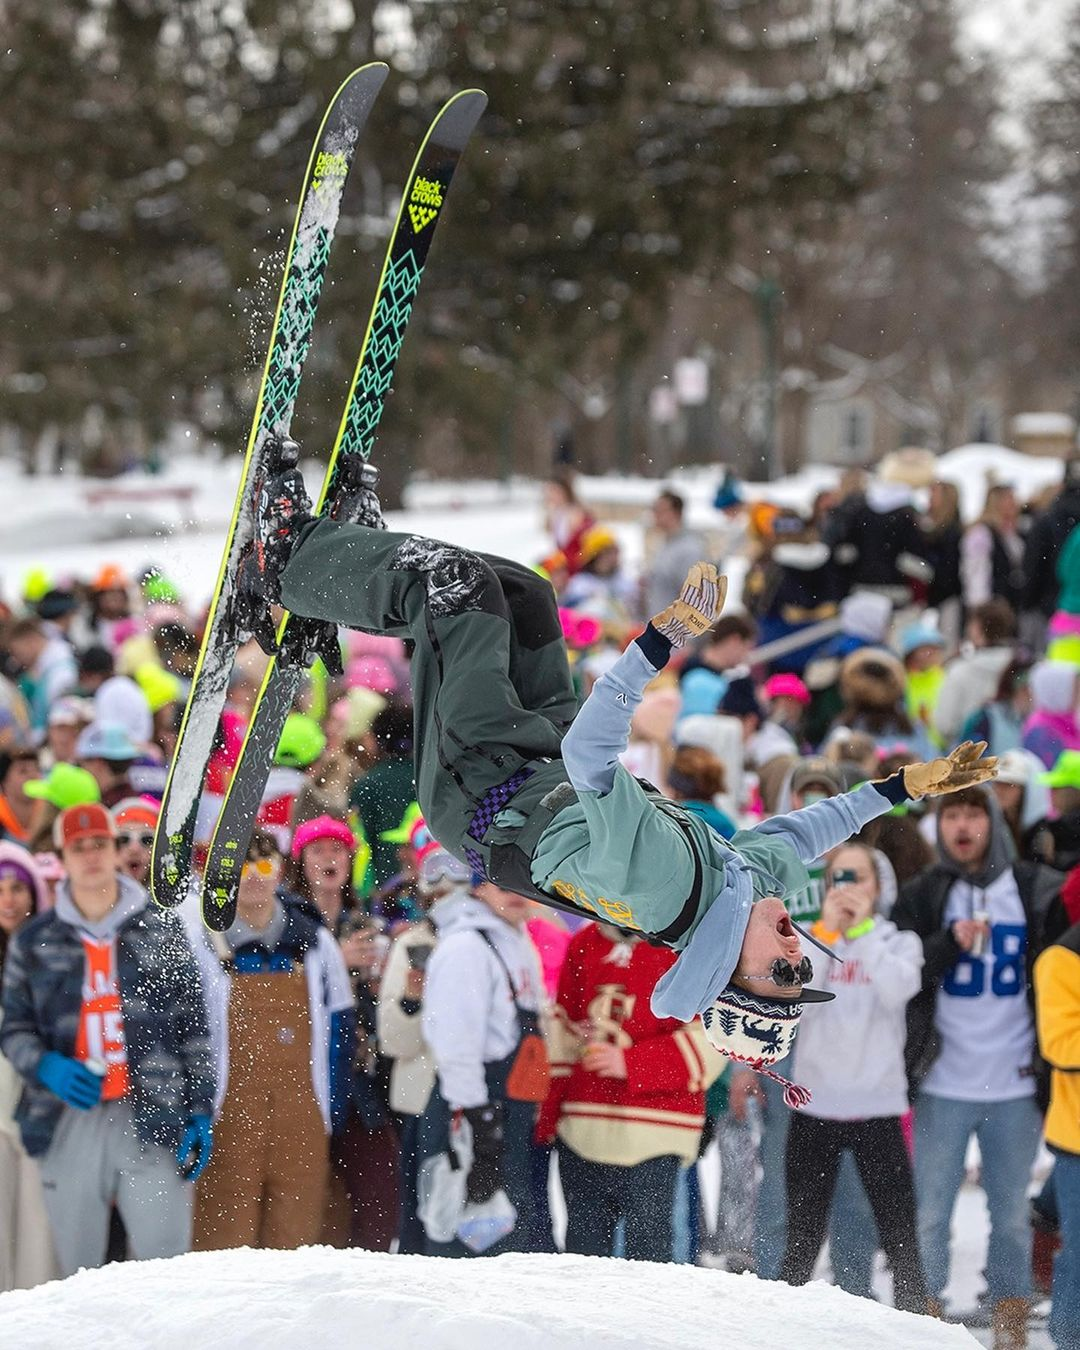
\includegraphics{images/TitusFlip.jpg}

}

\subcaption{\label{fig-grass_internet}Skiing Backflip(St.~Lawrence
University)}

\end{minipage}%
\newline
\begin{minipage}{0.50\linewidth}

\centering{

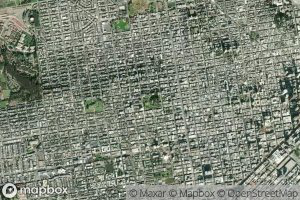
\includegraphics{images/san_francisco_scale_zoom_12.png}

}

\subcaption{\label{fig-sf}Downtown San Francisco, CA}

\end{minipage}%
%
\begin{minipage}{0.50\linewidth}

\centering{

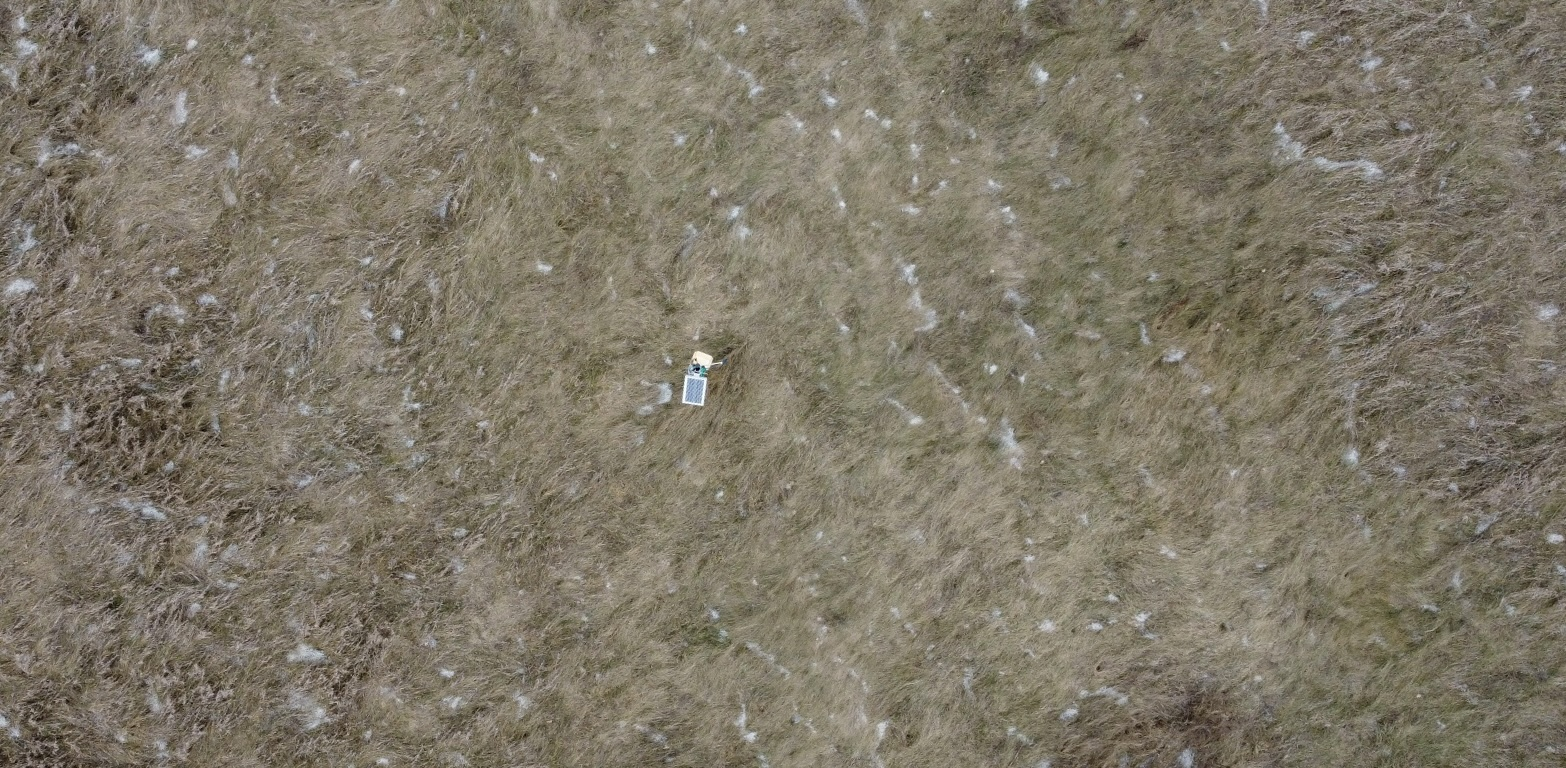
\includegraphics{images/living_lab_aerial/aerial_grass_living_lab_rotated.jpg}

}

\subcaption{\label{fig-living_labs}Aerial Grass Image(St.~Lawrence
University Living Laboratory)}

\end{minipage}%

\caption{\label{fig-images}Sample of Images for Evaluation}

\end{figure}%

\bookmarksetup{startatroot}

\chapter{Methods}\label{methods}

~~~~~~The HOG algorithm, introduced by Navneet Dalal and Bill Triggs in
2005, is a popular technique for object detection in images. The
algorithm can identify gradient magnitudes and angles at each pixel in
an image. The preliminary steps involved using the `skimage' library
from Python to preprocess the images of interest. This included loading,
resizing, and converting the images to grayscale. Images were rescaled
to standardize their resolutions and preserve their aspect ratios to
prevent distortion that could affect the accuracy of angle
identification. Converting the images to grayscale was necessary because
it allowed for focusing on a single channel to represent pixel
intensity, rather than three channels (red, green, and blue).

\begin{figure}

\begin{minipage}{\linewidth}

\centering{

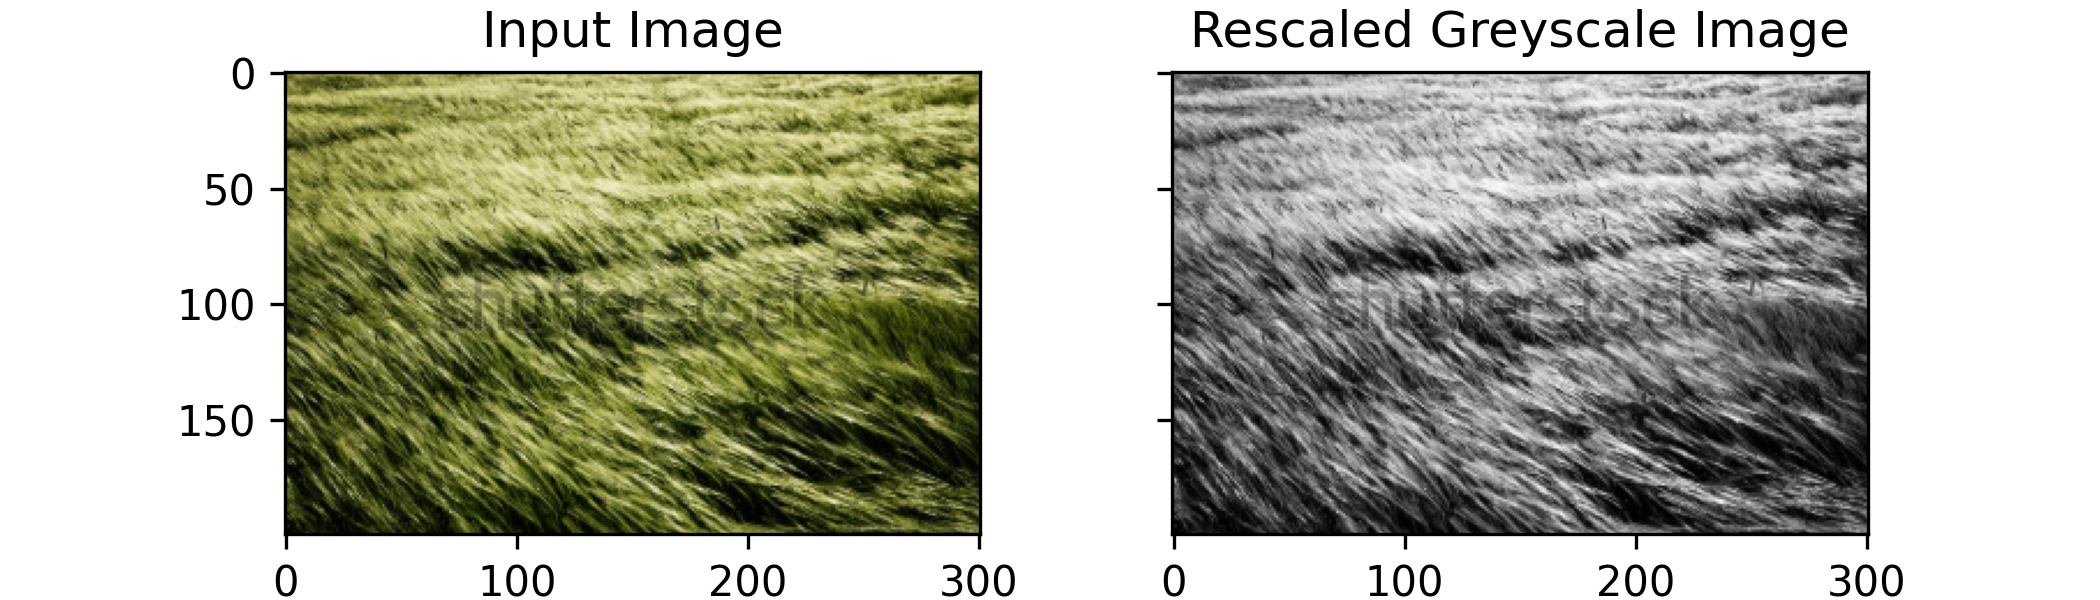
\includegraphics{images/plots/input_to_rescaled_plot.png}

}

\subcaption{\label{fig-input_image_to_new}Colored Image with Diagonal
Lines}

\end{minipage}%

\caption{\label{fig-input_image}Rescaling and Converting Image to
Greyscale}

\end{figure}%

~~~~~~The HOG features were then computed for the resized images, which
involved calculating the gradient magnitudes and angles at each pixel.
The gradient magnitude at each pixel is comprised of the gradients in
the `x' and `y' directions. The gradient in the x-direction is computed
by subtracting the pixel value to the left of pixel of interest is
subtracted from the pixel value to its right. Similarly, the gradient in
the y-direction is calculated by pixel value below the pixel of interest
is subtracted from the pixel value above the pixel of interest.

\(G_x=I(r,c+1)−I(r,c-1)\)

\(G_y=I(r+1,c)−I(r-1,c)\)

~~~~~~Now to calculate the gradient magnitude at the pixel of interest,
the Pythagorean Theorem can be utilized where the gradient magnitude is
equal to the square root of the x-gradient squared plus the y-gradient
squared. The angle at a given pixel can be calculated by taking the
inverse tangent of its y-gradient divided by its x-gradient. It is
important to note all angles produced by this algorithm are between zero
and one hundred eighty degrees. This occurs, because the inverse tangent
function used for calculating a given pixel's angle cannot distinguish
between all four quadrants.

\(Magnitude(\mu)=\sqrt{G_{x}^{2} + G_{y}^{2}}\)

\(Angle(\Theta)=tan^{−1} (\frac{G_y}{G_x})\)

\begin{figure}

\begin{minipage}{\linewidth}
\end{minipage}%
\newline
\begin{minipage}{\linewidth}

\centering{

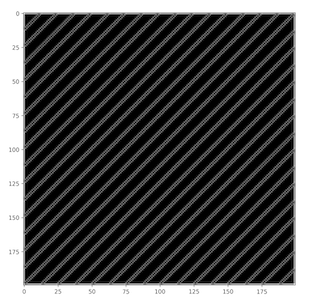
\includegraphics{images/plots/diagonal_lines_mag.png}

}

\subcaption{\label{fig-magnitude_grass}Gradient Magnitudes of Diagonal
Lines Image}

\end{minipage}%

\caption{\label{fig-mag_plot}Plotting Gradient Magnitudes as Image}

\end{figure}%

\hfill\break
~~~~~~Next, histograms are constructed to visualize the distribution of
gradient magnitudes and angles. Two different techniques for creating
gradient angle histograms were implemented. The first histogram was
created by counting the number of angles that fell into their respective
bins. The second scheme factors in a pixel's gradient magnitude and its
allocation to its bordering bins. Here, the weight assigned to each bin
is calculated by the angle's deviation from the center of its central
bin. This approach allows for a more representative histogram which
splits angles between bins and takes their magnitudes into account.
Lastly, these histograms are converted to polar histograms so the
primary angles can be visualized and compared to their original images.

\begin{figure}

\begin{minipage}{0.25\linewidth}

\begin{figure}[H]

{\centering 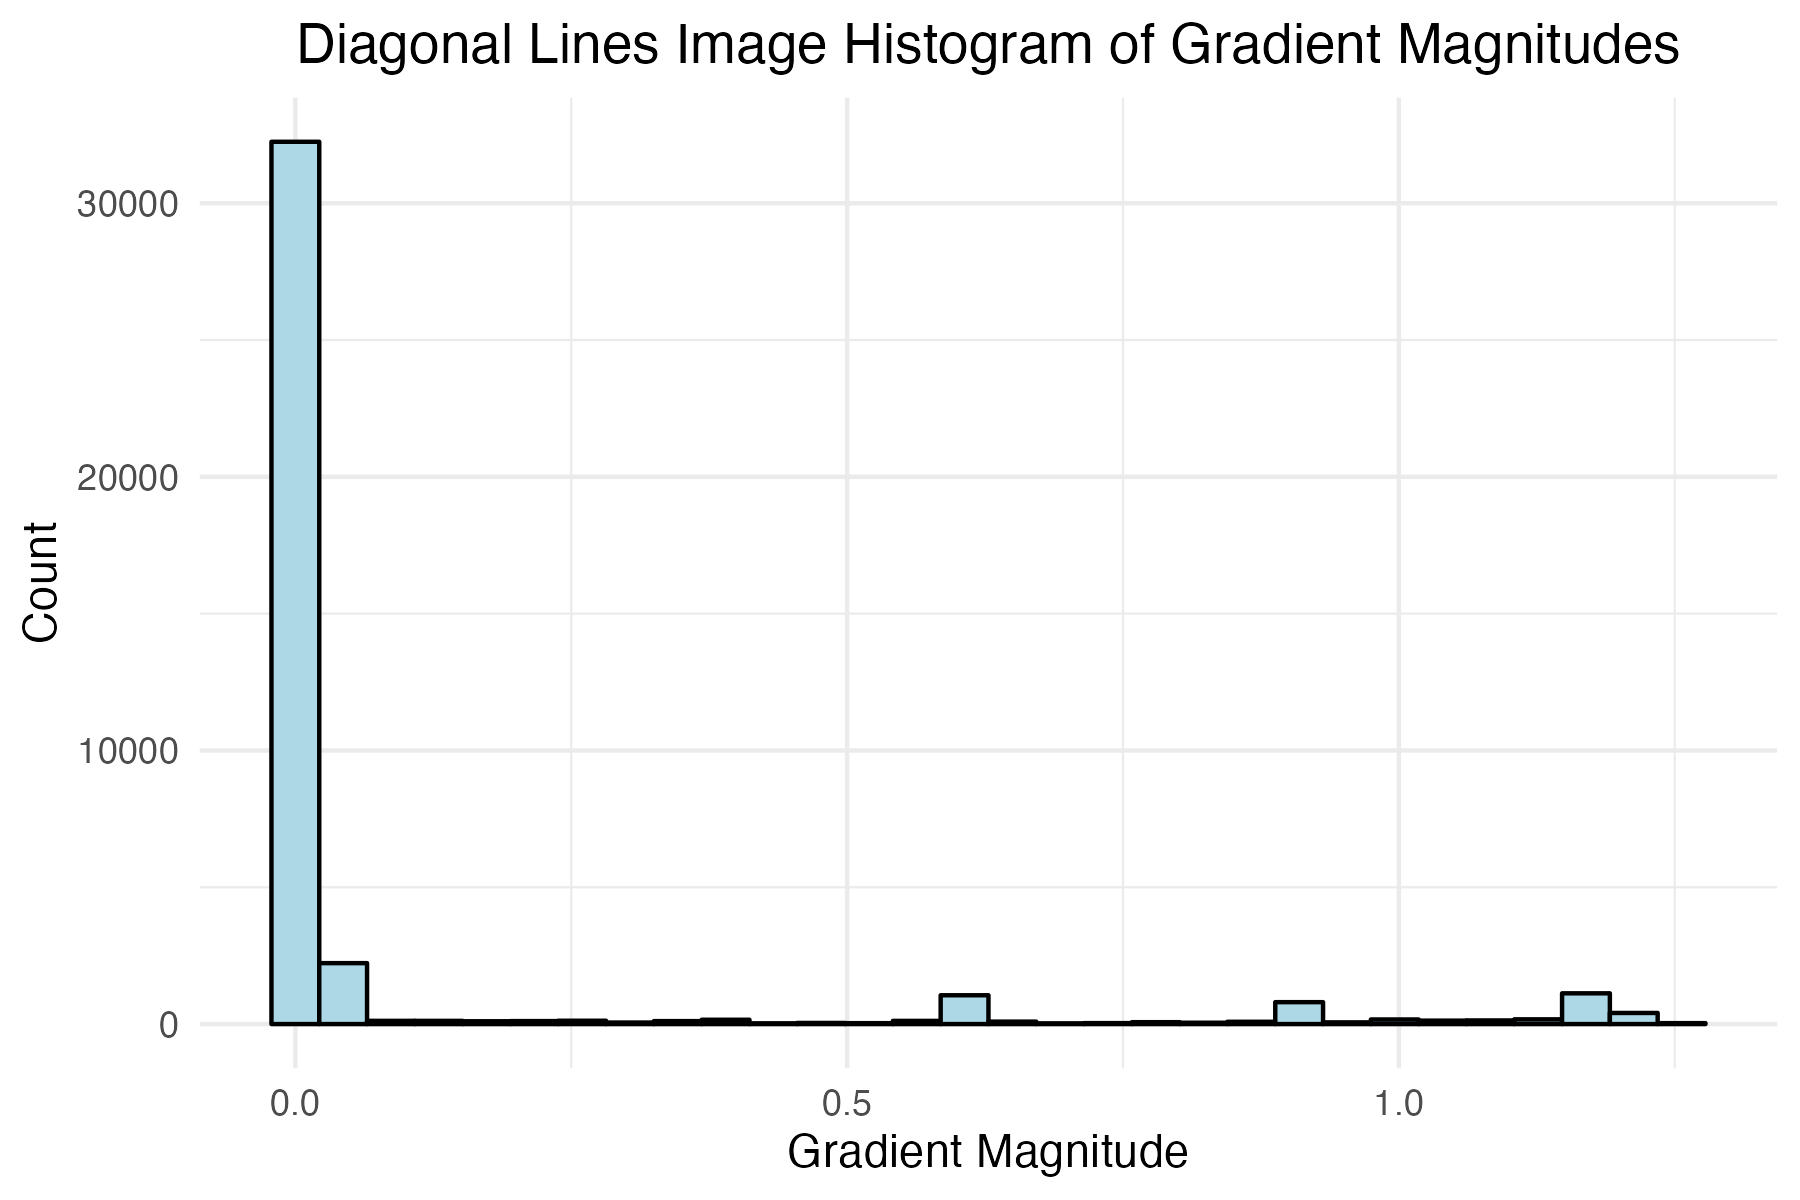
\includegraphics{images/plots/diagonal/diag_histogram_mag_plot.jpg}

}

\subcaption{Histograms of Gradient Magnitudes}

\end{figure}%

\end{minipage}%
%
\begin{minipage}{0.25\linewidth}

\begin{figure}[H]

{\centering 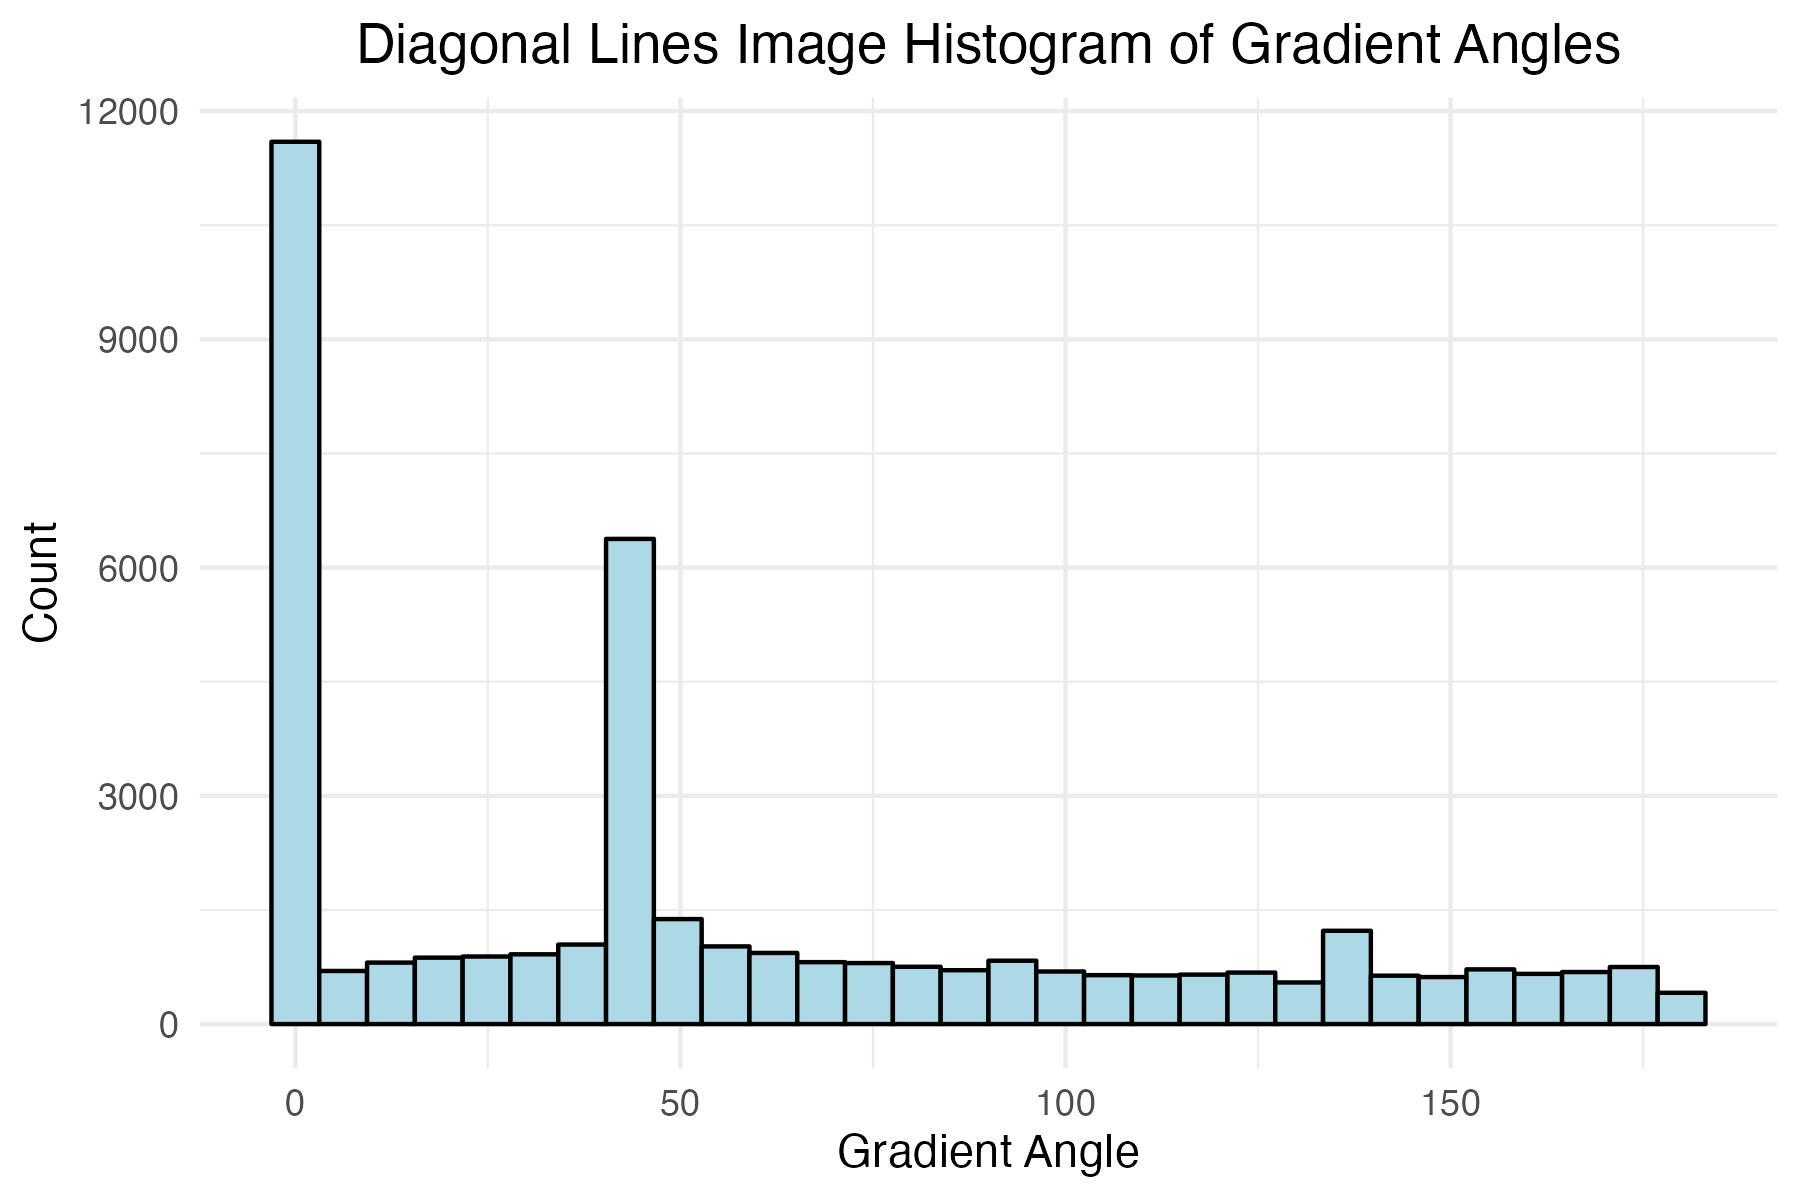
\includegraphics{images/plots/diagonal/diag_histogram_theta_plot.jpg}

}

\subcaption{Histograms of Gradient Angles}

\end{figure}%

\end{minipage}%
%
\begin{minipage}{0.25\linewidth}

\begin{figure}[H]

{\centering 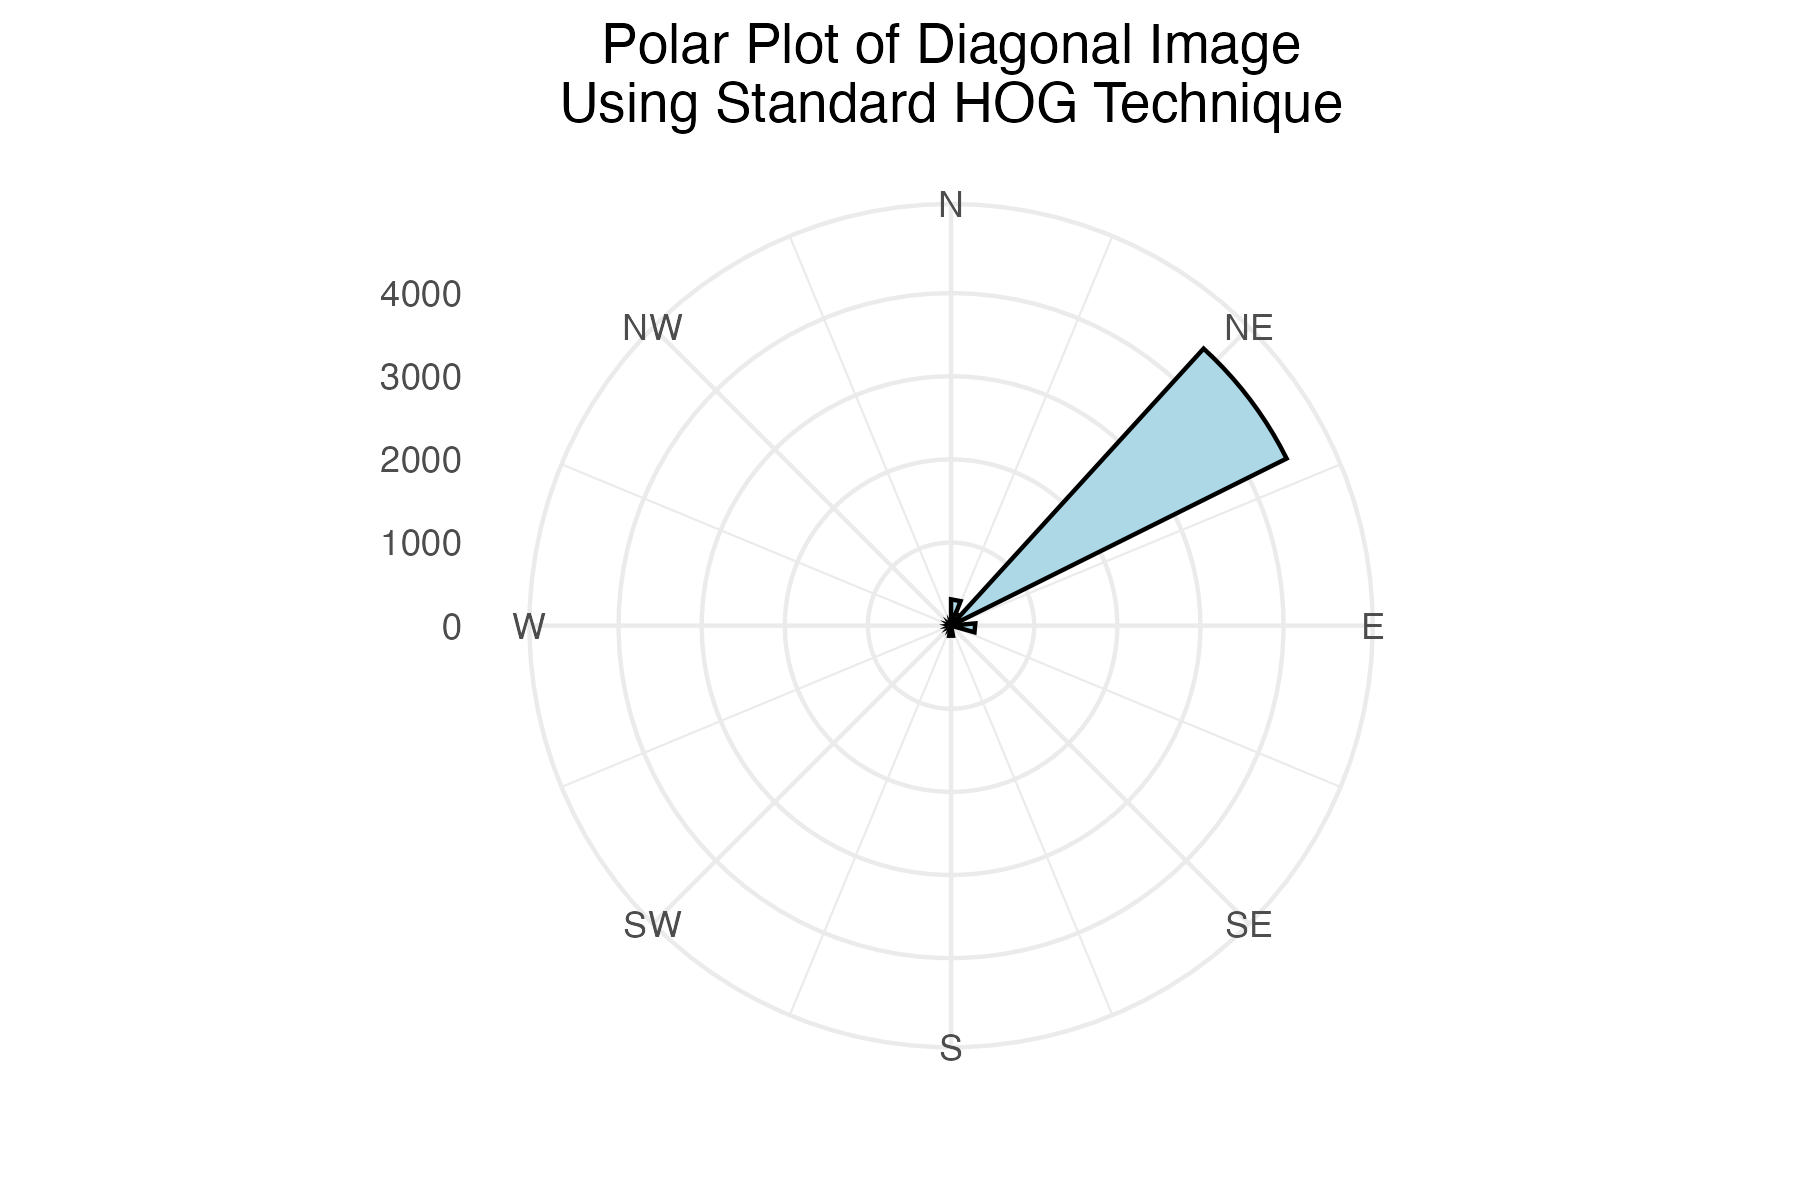
\includegraphics{images/plots/diagonal/diag_standard_polar_plot.jpg}

}

\subcaption{Polar Plot Using Standard Histogram Technique}

\end{figure}%

\end{minipage}%
%
\begin{minipage}{0.25\linewidth}

\begin{figure}[H]

{\centering 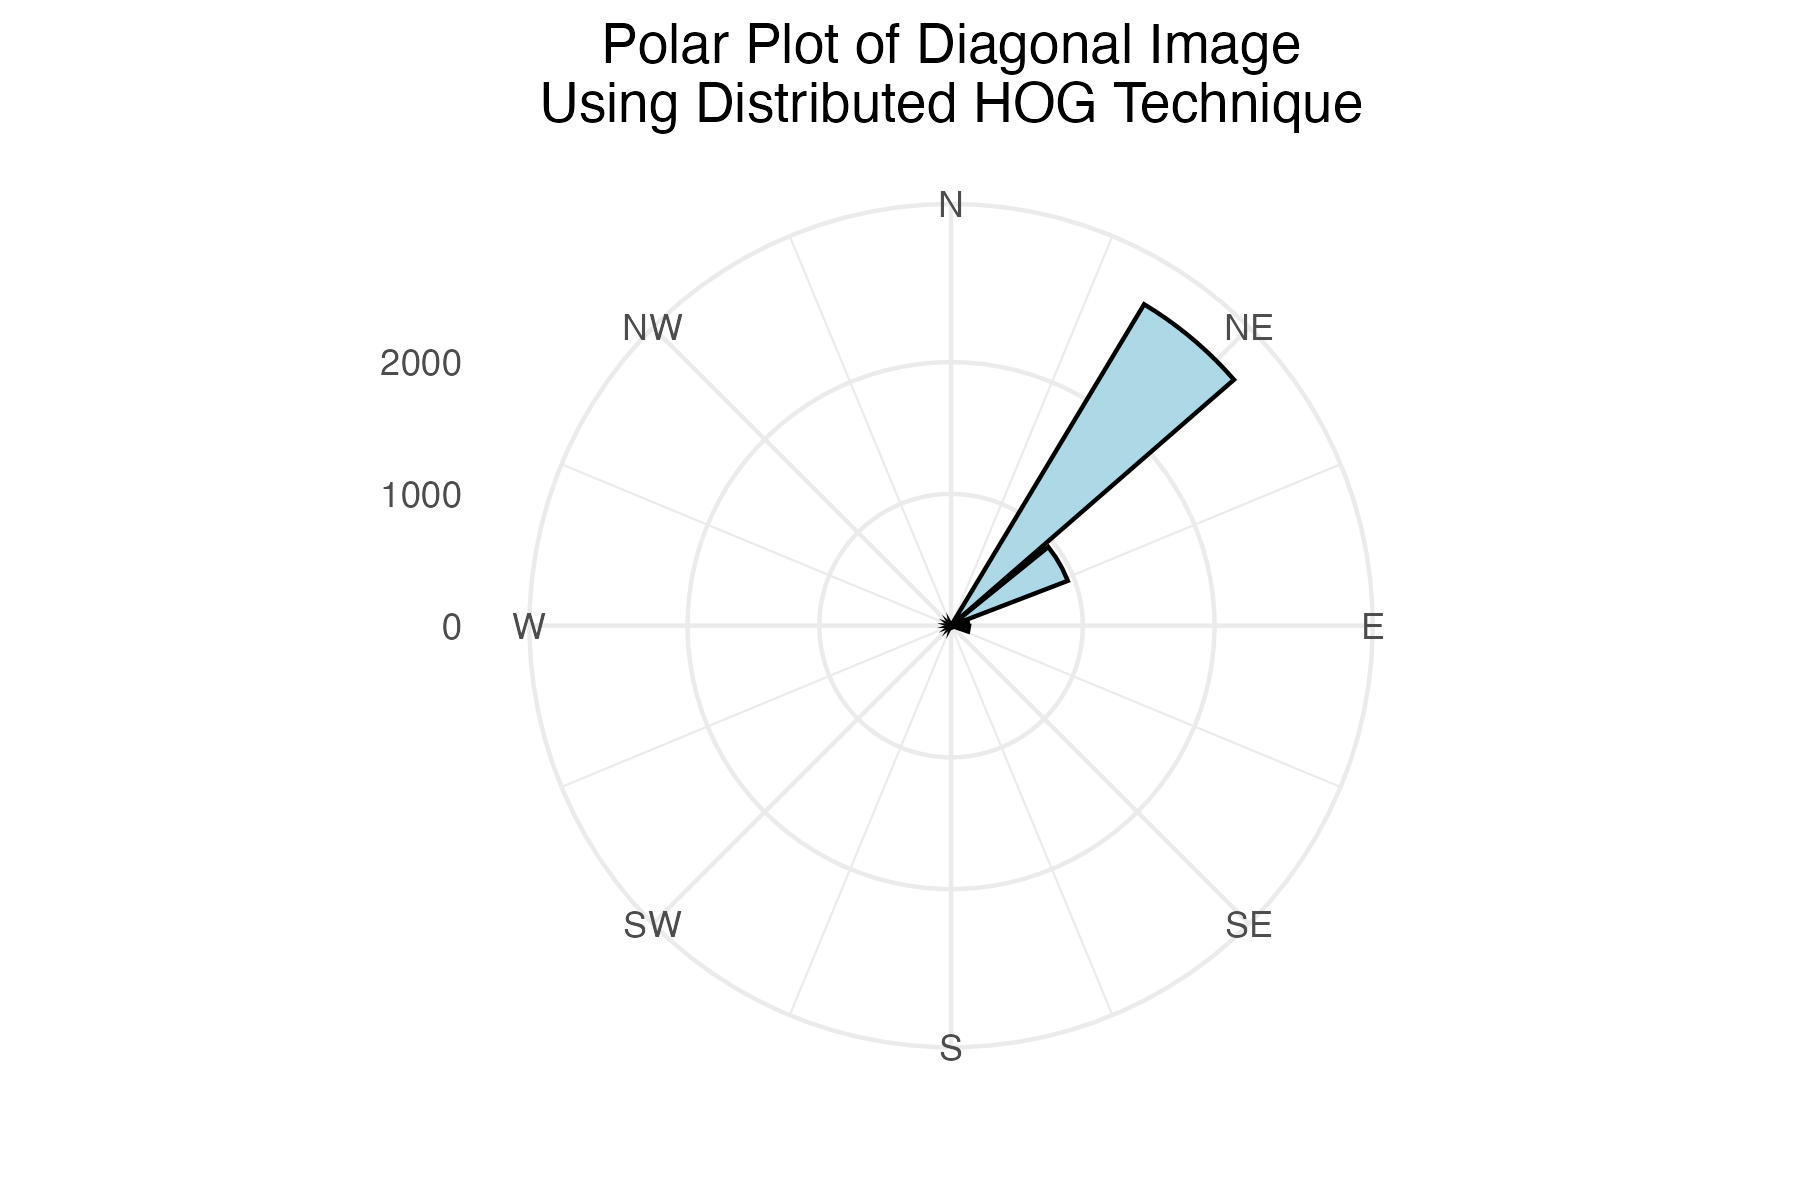
\includegraphics{images/plots/diagonal/diag_contribution_polar_plot.jpg}

}

\subcaption{Polar Plot Using Distributed Histogram Technique}

\end{figure}%

\end{minipage}%

\caption{\label{fig-histograms-plot-diag-line}Plotting Histograms of
Gradients}

\end{figure}%

\part{Results}

\chapter{Aerial Cityscapes}\label{aerial-cityscapes}

\section{Load R Packages and Python
Libraries}\label{load-r-packages-and-python-libraries}

\begin{Shaded}
\begin{Highlighting}[]
\CommentTok{\# Load R Packages}
\FunctionTok{library}\NormalTok{(reticulate)}
\FunctionTok{library}\NormalTok{(tidyverse)}
\FunctionTok{library}\NormalTok{(mapsapi)}
\FunctionTok{library}\NormalTok{(mapboxapi)}
\FunctionTok{library}\NormalTok{(magick)}
\end{Highlighting}
\end{Shaded}

\begin{Shaded}
\begin{Highlighting}[]
\CommentTok{\# Load Python Libraries}
\ImportTok{import}\NormalTok{ matplotlib.pyplot }\ImportTok{as}\NormalTok{ plt}
\ImportTok{import}\NormalTok{ pandas }\ImportTok{as}\NormalTok{ pd}
\ImportTok{from}\NormalTok{ skimage.io }\ImportTok{import}\NormalTok{ imread, imshow}
\ImportTok{from}\NormalTok{ skimage.transform }\ImportTok{import}\NormalTok{ resize}
\ImportTok{from}\NormalTok{ skimage.feature }\ImportTok{import}\NormalTok{ hog}
\ImportTok{from}\NormalTok{ skimage }\ImportTok{import}\NormalTok{ data, exposure}
\ImportTok{import}\NormalTok{ matplotlib.pyplot }\ImportTok{as}\NormalTok{ plt}
\ImportTok{from}\NormalTok{ skimage }\ImportTok{import}\NormalTok{ io}
\ImportTok{from}\NormalTok{ skimage }\ImportTok{import}\NormalTok{ color}
\ImportTok{from}\NormalTok{ skimage.transform }\ImportTok{import}\NormalTok{ resize}
\ImportTok{import}\NormalTok{ math}
\ImportTok{from}\NormalTok{ skimage.feature }\ImportTok{import}\NormalTok{ hog}
\ImportTok{import}\NormalTok{ numpy }\ImportTok{as}\NormalTok{ np}
\end{Highlighting}
\end{Shaded}

\section{Download Aerial City Images from
Mapbox}\label{download-aerial-city-images-from-mapbox}

\begin{Shaded}
\begin{Highlighting}[]
\CommentTok{\# Get Mapbox token from System Environment }
\NormalTok{key }\OtherTok{\textless{}{-}} \FunctionTok{Sys.getenv}\NormalTok{(}\StringTok{"mapbox\_key"}\NormalTok{) }
\end{Highlighting}
\end{Shaded}

\begin{Shaded}
\begin{Highlighting}[]
\CommentTok{\# Download map of San Francisco, CA}
\NormalTok{map }\OtherTok{\textless{}{-}} \FunctionTok{static\_mapbox}\NormalTok{(}
  \AttributeTok{access\_token =}\NormalTok{ key,}
  \AttributeTok{style\_url =} \StringTok{"mapbox://styles/mapbox/satellite{-}v9"}\NormalTok{,}
  \AttributeTok{width =} \DecValTok{300}\NormalTok{,}
  \AttributeTok{height =} \DecValTok{200}\NormalTok{, }
  \AttributeTok{image =}\NormalTok{ T, }\AttributeTok{latitude =} \FloatTok{37.792004}\NormalTok{, }\AttributeTok{longitude =} \SpecialCharTok{{-}}\FloatTok{122.428079}\NormalTok{, }\AttributeTok{zoom =} \DecValTok{12}
\NormalTok{)}

\NormalTok{magick}\SpecialCharTok{::}\FunctionTok{image\_write}\NormalTok{(map, }\StringTok{"images/san\_francisco\_scale\_zoom\_12.png"}\NormalTok{)}
\end{Highlighting}
\end{Shaded}

\begin{Shaded}
\begin{Highlighting}[]
\CommentTok{\# Download map of Salt Lake City, UT}
\NormalTok{points\_of\_interest }\OtherTok{\textless{}{-}}\NormalTok{ tibble}\SpecialCharTok{::}\FunctionTok{tibble}\NormalTok{(}
  \AttributeTok{longitude =} \FunctionTok{c}\NormalTok{(}\SpecialCharTok{{-}}\FloatTok{112.065945}\NormalTok{, }\SpecialCharTok{{-}}\FloatTok{111.853948}\NormalTok{, }
                \SpecialCharTok{{-}}\FloatTok{111.852956}\NormalTok{, }\SpecialCharTok{{-}}\FloatTok{112.023371}\NormalTok{),}
  
  \AttributeTok{latitude =} \FunctionTok{c}\NormalTok{(}\FloatTok{40.794275}\NormalTok{, }\FloatTok{40.791516}\NormalTok{, }
               \FloatTok{40.502308}\NormalTok{, }\FloatTok{40.502308}\NormalTok{)}
\NormalTok{  )}

\NormalTok{prepped\_pois }\OtherTok{\textless{}{-}} \FunctionTok{prep\_overlay\_markers}\NormalTok{(}
  \AttributeTok{data =}\NormalTok{ points\_of\_interest,}
  \AttributeTok{marker\_type =} \StringTok{"pin{-}l"}\NormalTok{,}
  \AttributeTok{label =} \DecValTok{1}\SpecialCharTok{:}\DecValTok{4}\NormalTok{,}
  \AttributeTok{color =} \StringTok{"\#fff"}\NormalTok{, }
\NormalTok{)}

\NormalTok{map }\OtherTok{\textless{}{-}} \FunctionTok{static\_mapbox}\NormalTok{(}
  \AttributeTok{access\_token =}\NormalTok{ key,}
  \AttributeTok{style\_url =} \StringTok{"mapbox://styles/mapbox/satellite{-}v9"}\NormalTok{,}
  \AttributeTok{width =} \DecValTok{800}\NormalTok{,}
  \AttributeTok{height =} \DecValTok{1200}\NormalTok{, }
  \AttributeTok{image =}\NormalTok{ T, }
  \AttributeTok{latitude =} \FloatTok{40.7}\NormalTok{,}
  \AttributeTok{longitude =} \SpecialCharTok{{-}}\FloatTok{111.876183}\NormalTok{, }\AttributeTok{zoom =} \DecValTok{12}
\NormalTok{)}

\NormalTok{magick}\SpecialCharTok{::}\FunctionTok{image\_write}\NormalTok{(map, }\StringTok{"images/salt\_lake\_city\_zoom\_12.png"}\NormalTok{)}
\end{Highlighting}
\end{Shaded}

\begin{Shaded}
\begin{Highlighting}[]
\CommentTok{\# Download map of Detroit, MI}
\NormalTok{map }\OtherTok{\textless{}{-}} \FunctionTok{static\_mapbox}\NormalTok{(}
  \AttributeTok{access\_token =}\NormalTok{ key,}
  \AttributeTok{style\_url =} \StringTok{"mapbox://styles/mapbox/satellite{-}v9"}\NormalTok{,}
  \AttributeTok{width =} \DecValTok{1200}\NormalTok{,}
  \AttributeTok{height =} \DecValTok{800}\NormalTok{, }
  \AttributeTok{image =}\NormalTok{ T, }
  \AttributeTok{latitude =} \FloatTok{42.336322}\NormalTok{,}
  \AttributeTok{longitude =} \SpecialCharTok{{-}}\FloatTok{83.048705}\NormalTok{, }\AttributeTok{zoom =} \DecValTok{12}
\NormalTok{)}

\NormalTok{magick}\SpecialCharTok{::}\FunctionTok{image\_write}\NormalTok{(map, }\StringTok{"images/detroit\_zoom\_12.png"}\NormalTok{)}
\end{Highlighting}
\end{Shaded}

\begin{figure}

\begin{minipage}{0.33\linewidth}

\begin{figure}[H]

{\centering 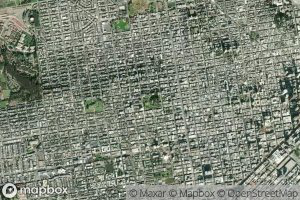
\includegraphics{images/san_francisco_scale_zoom_12.png}

}

\subcaption{San Francisco Cityscape}

\end{figure}%

\end{minipage}%
%
\begin{minipage}{0.33\linewidth}

\begin{figure}[H]

{\centering 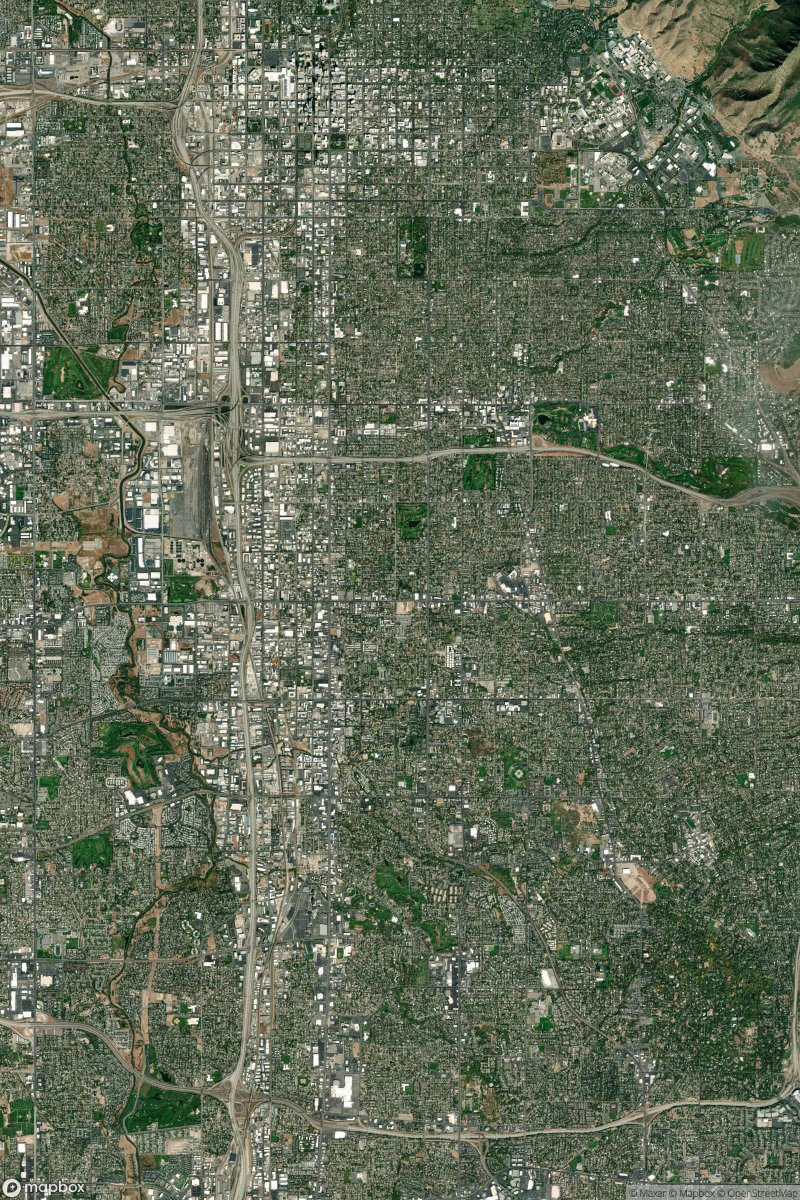
\includegraphics{images/salt_lake_city_zoom_12.png}

}

\subcaption{Salt Lake City Cityscape}

\end{figure}%

\end{minipage}%
%
\begin{minipage}{0.33\linewidth}

\begin{figure}[H]

{\centering 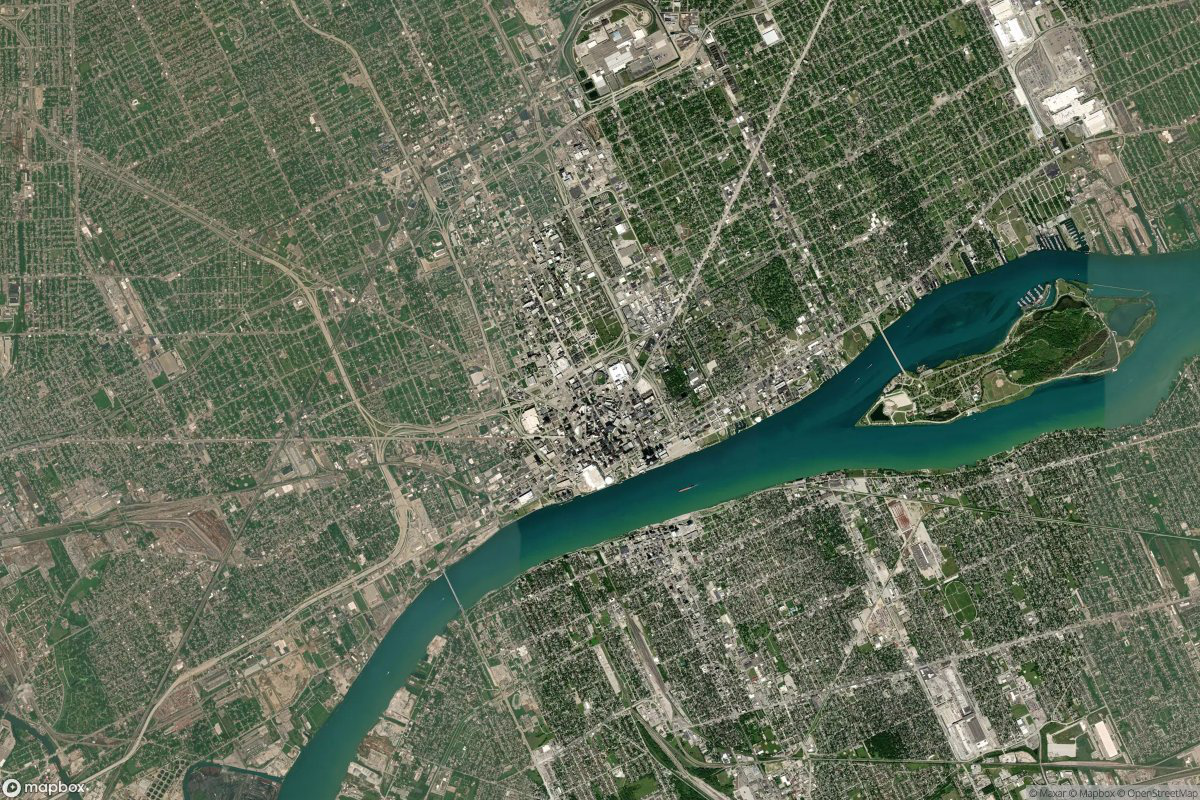
\includegraphics{images/detroit_zoom_12.png}

}

\subcaption{Detroit Cityscape}

\end{figure}%

\end{minipage}%

\caption{\label{fig-city-images}Aerial Cityscape Images}

\end{figure}%

\section{Collect HOG Features for Aerial
Cityscapes}\label{collect-hog-features-for-aerial-cityscapes}

\begin{Shaded}
\begin{Highlighting}[]
\CommentTok{\# List for storing images}
\NormalTok{img\_list }\OperatorTok{=}\NormalTok{ []}

\CommentTok{\# SF aerial}
\NormalTok{img\_list.append(color.rgb2gray(io.imread(}\StringTok{"images/san\_francisco\_scale\_zoom\_12.png"}\NormalTok{)))}

\CommentTok{\# Salt Lake City Aerial}
\NormalTok{img\_list.append(color.rgb2gray(io.imread(}\StringTok{"images/salt\_lake\_city\_zoom\_12.png"}\NormalTok{)))}

\CommentTok{\# Detroit Aerial}
\NormalTok{img\_list.append(color.rgb2gray(io.imread(}\StringTok{"images/detroit\_zoom\_12.png"}\NormalTok{)))}

\CommentTok{\# List to store magnitudes for each image}
\NormalTok{mag\_list }\OperatorTok{=}\NormalTok{ []}

\CommentTok{\# List to store angles for each image}
\NormalTok{theta\_list }\OperatorTok{=}\NormalTok{ []}


\ControlFlowTok{for}\NormalTok{ x }\KeywordTok{in} \BuiltInTok{range}\NormalTok{(}\BuiltInTok{len}\NormalTok{(img\_list)):}
    \CommentTok{\# Get image of interest}
\NormalTok{    img }\OperatorTok{=}\NormalTok{ img\_list[x]}
    
\NormalTok{    rescaled\_file\_path }\OperatorTok{=} \SpecialStringTok{f"images/plots/aerial\_cities/}\SpecialCharTok{\{}\NormalTok{x}\SpecialCharTok{\}}\SpecialStringTok{.jpg"}
    
    \CommentTok{\# Determine aspect Ratio}
\NormalTok{    aspect\_ratio }\OperatorTok{=}\NormalTok{ img.shape[}\DecValTok{0}\NormalTok{] }\OperatorTok{/}\NormalTok{ img.shape[}\DecValTok{1}\NormalTok{]}
    \BuiltInTok{print}\NormalTok{(}\StringTok{"Aspect Ratio:"}\NormalTok{, aspect\_ratio)}
    
    \CommentTok{\# Hard{-}Code height to 200 pixels}
\NormalTok{    height }\OperatorTok{=} \DecValTok{200}
    
    \CommentTok{\# Calculate witdth to maintain same aspect ratio}
\NormalTok{    width }\OperatorTok{=} \BuiltInTok{int}\NormalTok{(height }\OperatorTok{/}\NormalTok{ aspect\_ratio)}
    \BuiltInTok{print}\NormalTok{(}\StringTok{"Resized Width:"}\NormalTok{, width)}
    
    \CommentTok{\# Resize the image}
\NormalTok{    resized\_img }\OperatorTok{=}\NormalTok{ resize(img, (height, width))}
    
    \CommentTok{\# Replace the original image with the resized image}
\NormalTok{    img\_list[x] }\OperatorTok{=}\NormalTok{ resized\_img}
    
    \CommentTok{\# if (x == 1):}
    \CommentTok{\#   plot\_width = 8}
    \CommentTok{\#   plot\_height = 15}
    \CommentTok{\# else:}
    \CommentTok{\#   plot\_width = 15}
    \CommentTok{\#   plot\_height = 9}
    \CommentTok{\# }
    \CommentTok{\# plt.figure(figsize=(plot\_width, plot\_height))}
    \CommentTok{\# plt.imshow(resized\_img, cmap="gray")}
    \CommentTok{\# plt.axis("on")}
    \CommentTok{\# plt.tight\_layout()}
    \CommentTok{\# plt.savefig(rescaled\_file\_path, dpi=300)}
    \CommentTok{\# plt.show()}

    
    \CommentTok{\# list for storing all magnitudes for image[x]}
\NormalTok{    mag }\OperatorTok{=}\NormalTok{ []}
    
    \CommentTok{\# list for storing all angles for image[x]}
\NormalTok{    theta }\OperatorTok{=}\NormalTok{ []}
    
    \ControlFlowTok{for}\NormalTok{ i }\KeywordTok{in} \BuiltInTok{range}\NormalTok{(height):}
\NormalTok{        magnitudeArray }\OperatorTok{=}\NormalTok{ []}
\NormalTok{        angleArray }\OperatorTok{=}\NormalTok{ []}

        \ControlFlowTok{for}\NormalTok{ j }\KeywordTok{in} \BuiltInTok{range}\NormalTok{(width):}
            \ControlFlowTok{if}\NormalTok{ j }\OperatorTok{{-}} \DecValTok{1} \OperatorTok{\textless{}} \DecValTok{0} \KeywordTok{or}\NormalTok{ j }\OperatorTok{+} \DecValTok{1} \OperatorTok{\textgreater{}=}\NormalTok{ width:}
                \ControlFlowTok{if}\NormalTok{ j }\OperatorTok{{-}} \DecValTok{1} \OperatorTok{\textless{}} \DecValTok{0}\NormalTok{:}
\NormalTok{                    Gx }\OperatorTok{=}\NormalTok{ resized\_img[i][j }\OperatorTok{+} \DecValTok{1}\NormalTok{] }\OperatorTok{{-}} \DecValTok{0}
                \ControlFlowTok{elif}\NormalTok{ j }\OperatorTok{+} \DecValTok{1} \OperatorTok{\textgreater{}=}\NormalTok{ width:}
\NormalTok{                    Gx }\OperatorTok{=} \DecValTok{0} \OperatorTok{{-}}\NormalTok{ resized\_img[i][j }\OperatorTok{{-}} \DecValTok{1}\NormalTok{]}
            \ControlFlowTok{else}\NormalTok{:}
\NormalTok{                Gx }\OperatorTok{=}\NormalTok{ resized\_img[i][j }\OperatorTok{+} \DecValTok{1}\NormalTok{] }\OperatorTok{{-}}\NormalTok{ resized\_img[i][j }\OperatorTok{{-}} \DecValTok{1}\NormalTok{]}

            \ControlFlowTok{if}\NormalTok{ i }\OperatorTok{{-}} \DecValTok{1} \OperatorTok{\textless{}} \DecValTok{0} \KeywordTok{or}\NormalTok{ i }\OperatorTok{+} \DecValTok{1} \OperatorTok{\textgreater{}=}\NormalTok{ height:}
                \ControlFlowTok{if}\NormalTok{ i }\OperatorTok{{-}} \DecValTok{1} \OperatorTok{\textless{}} \DecValTok{0}\NormalTok{:}
\NormalTok{                    Gy }\OperatorTok{=} \DecValTok{0} \OperatorTok{{-}}\NormalTok{ resized\_img[i }\OperatorTok{+} \DecValTok{1}\NormalTok{][j]}
                \ControlFlowTok{elif}\NormalTok{ i }\OperatorTok{+} \DecValTok{1} \OperatorTok{\textgreater{}=}\NormalTok{ height:}
\NormalTok{                    Gy }\OperatorTok{=}\NormalTok{ resized\_img[i }\OperatorTok{{-}} \DecValTok{1}\NormalTok{][j] }\OperatorTok{{-}} \DecValTok{0}
            \ControlFlowTok{else}\NormalTok{:}
\NormalTok{                Gy }\OperatorTok{=}\NormalTok{ resized\_img[i }\OperatorTok{+} \DecValTok{1}\NormalTok{][j] }\OperatorTok{{-}}\NormalTok{ resized\_img[i }\OperatorTok{{-}} \DecValTok{1}\NormalTok{][j]}

\NormalTok{            magnitude }\OperatorTok{=}\NormalTok{ math.sqrt(}\BuiltInTok{pow}\NormalTok{(Gx, }\DecValTok{2}\NormalTok{) }\OperatorTok{+} \BuiltInTok{pow}\NormalTok{(Gy, }\DecValTok{2}\NormalTok{))}
\NormalTok{            magnitudeArray.append(}\BuiltInTok{round}\NormalTok{(magnitude, }\DecValTok{9}\NormalTok{))}

            \ControlFlowTok{if}\NormalTok{ Gx }\OperatorTok{==} \DecValTok{0}\NormalTok{:}
\NormalTok{                angle }\OperatorTok{=}\NormalTok{ math.degrees(}\FloatTok{0.0}\NormalTok{)}
            \ControlFlowTok{else}\NormalTok{:}
\NormalTok{                angle }\OperatorTok{=}\NormalTok{ math.degrees(math.atan(Gy }\OperatorTok{/}\NormalTok{ Gx))}
                \ControlFlowTok{if}\NormalTok{ angle }\OperatorTok{\textless{}} \DecValTok{0}\NormalTok{:}
\NormalTok{                    angle }\OperatorTok{+=} \DecValTok{180}

\NormalTok{            angleArray.append(}\BuiltInTok{round}\NormalTok{(angle, }\DecValTok{9}\NormalTok{))}

\NormalTok{        mag.append(magnitudeArray)}
\NormalTok{        theta.append(angleArray)}

    \CommentTok{\# add list of magnitudes to list[x]}
\NormalTok{    mag\_list.append(mag)}

    \CommentTok{\# add list of angles to angle list[x]}
\NormalTok{    theta\_list.append(theta)}
\end{Highlighting}
\end{Shaded}

\begin{verbatim}
Aspect Ratio: 0.6666666666666666
Resized Width: 300
Aspect Ratio: 1.5
Resized Width: 133
Aspect Ratio: 0.6666666666666666
Resized Width: 300
\end{verbatim}

\begin{figure}

\begin{minipage}{0.33\linewidth}

\begin{figure}[H]

{\centering 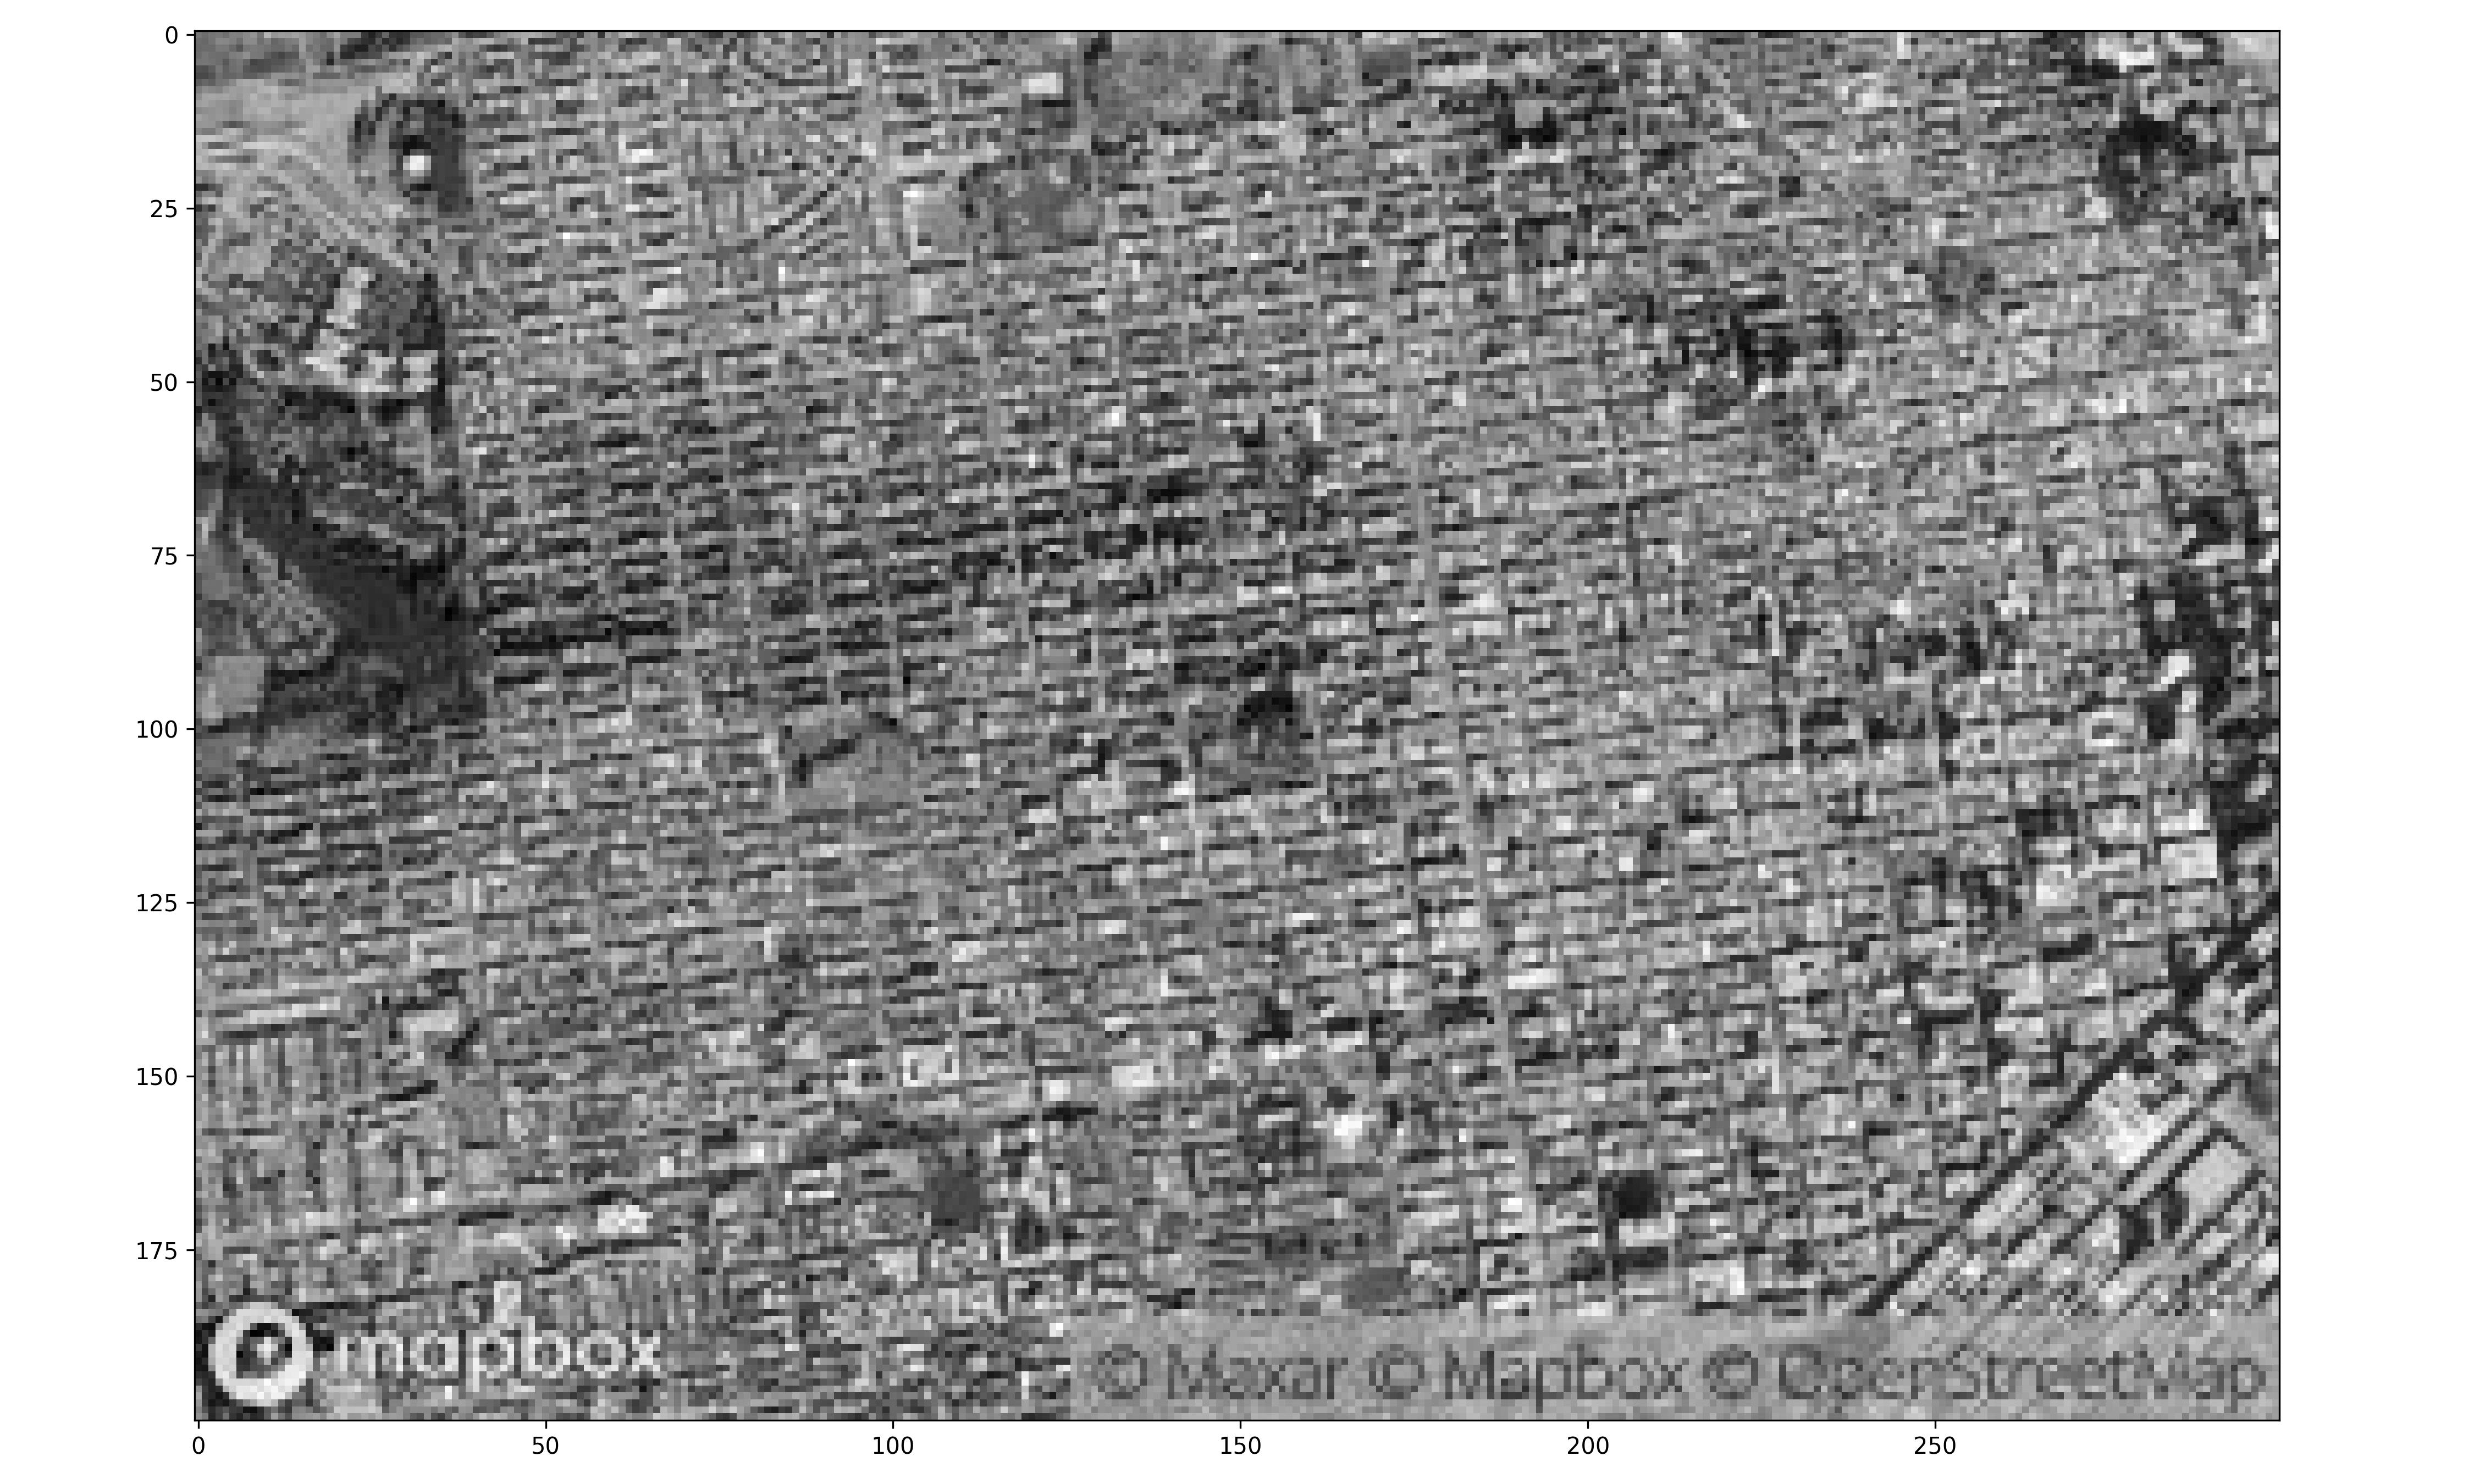
\includegraphics{images/plots/aerial_cities/0.jpg}

}

\subcaption{San Francisco, CA}

\end{figure}%

\end{minipage}%
%
\begin{minipage}{0.33\linewidth}

\begin{figure}[H]

{\centering 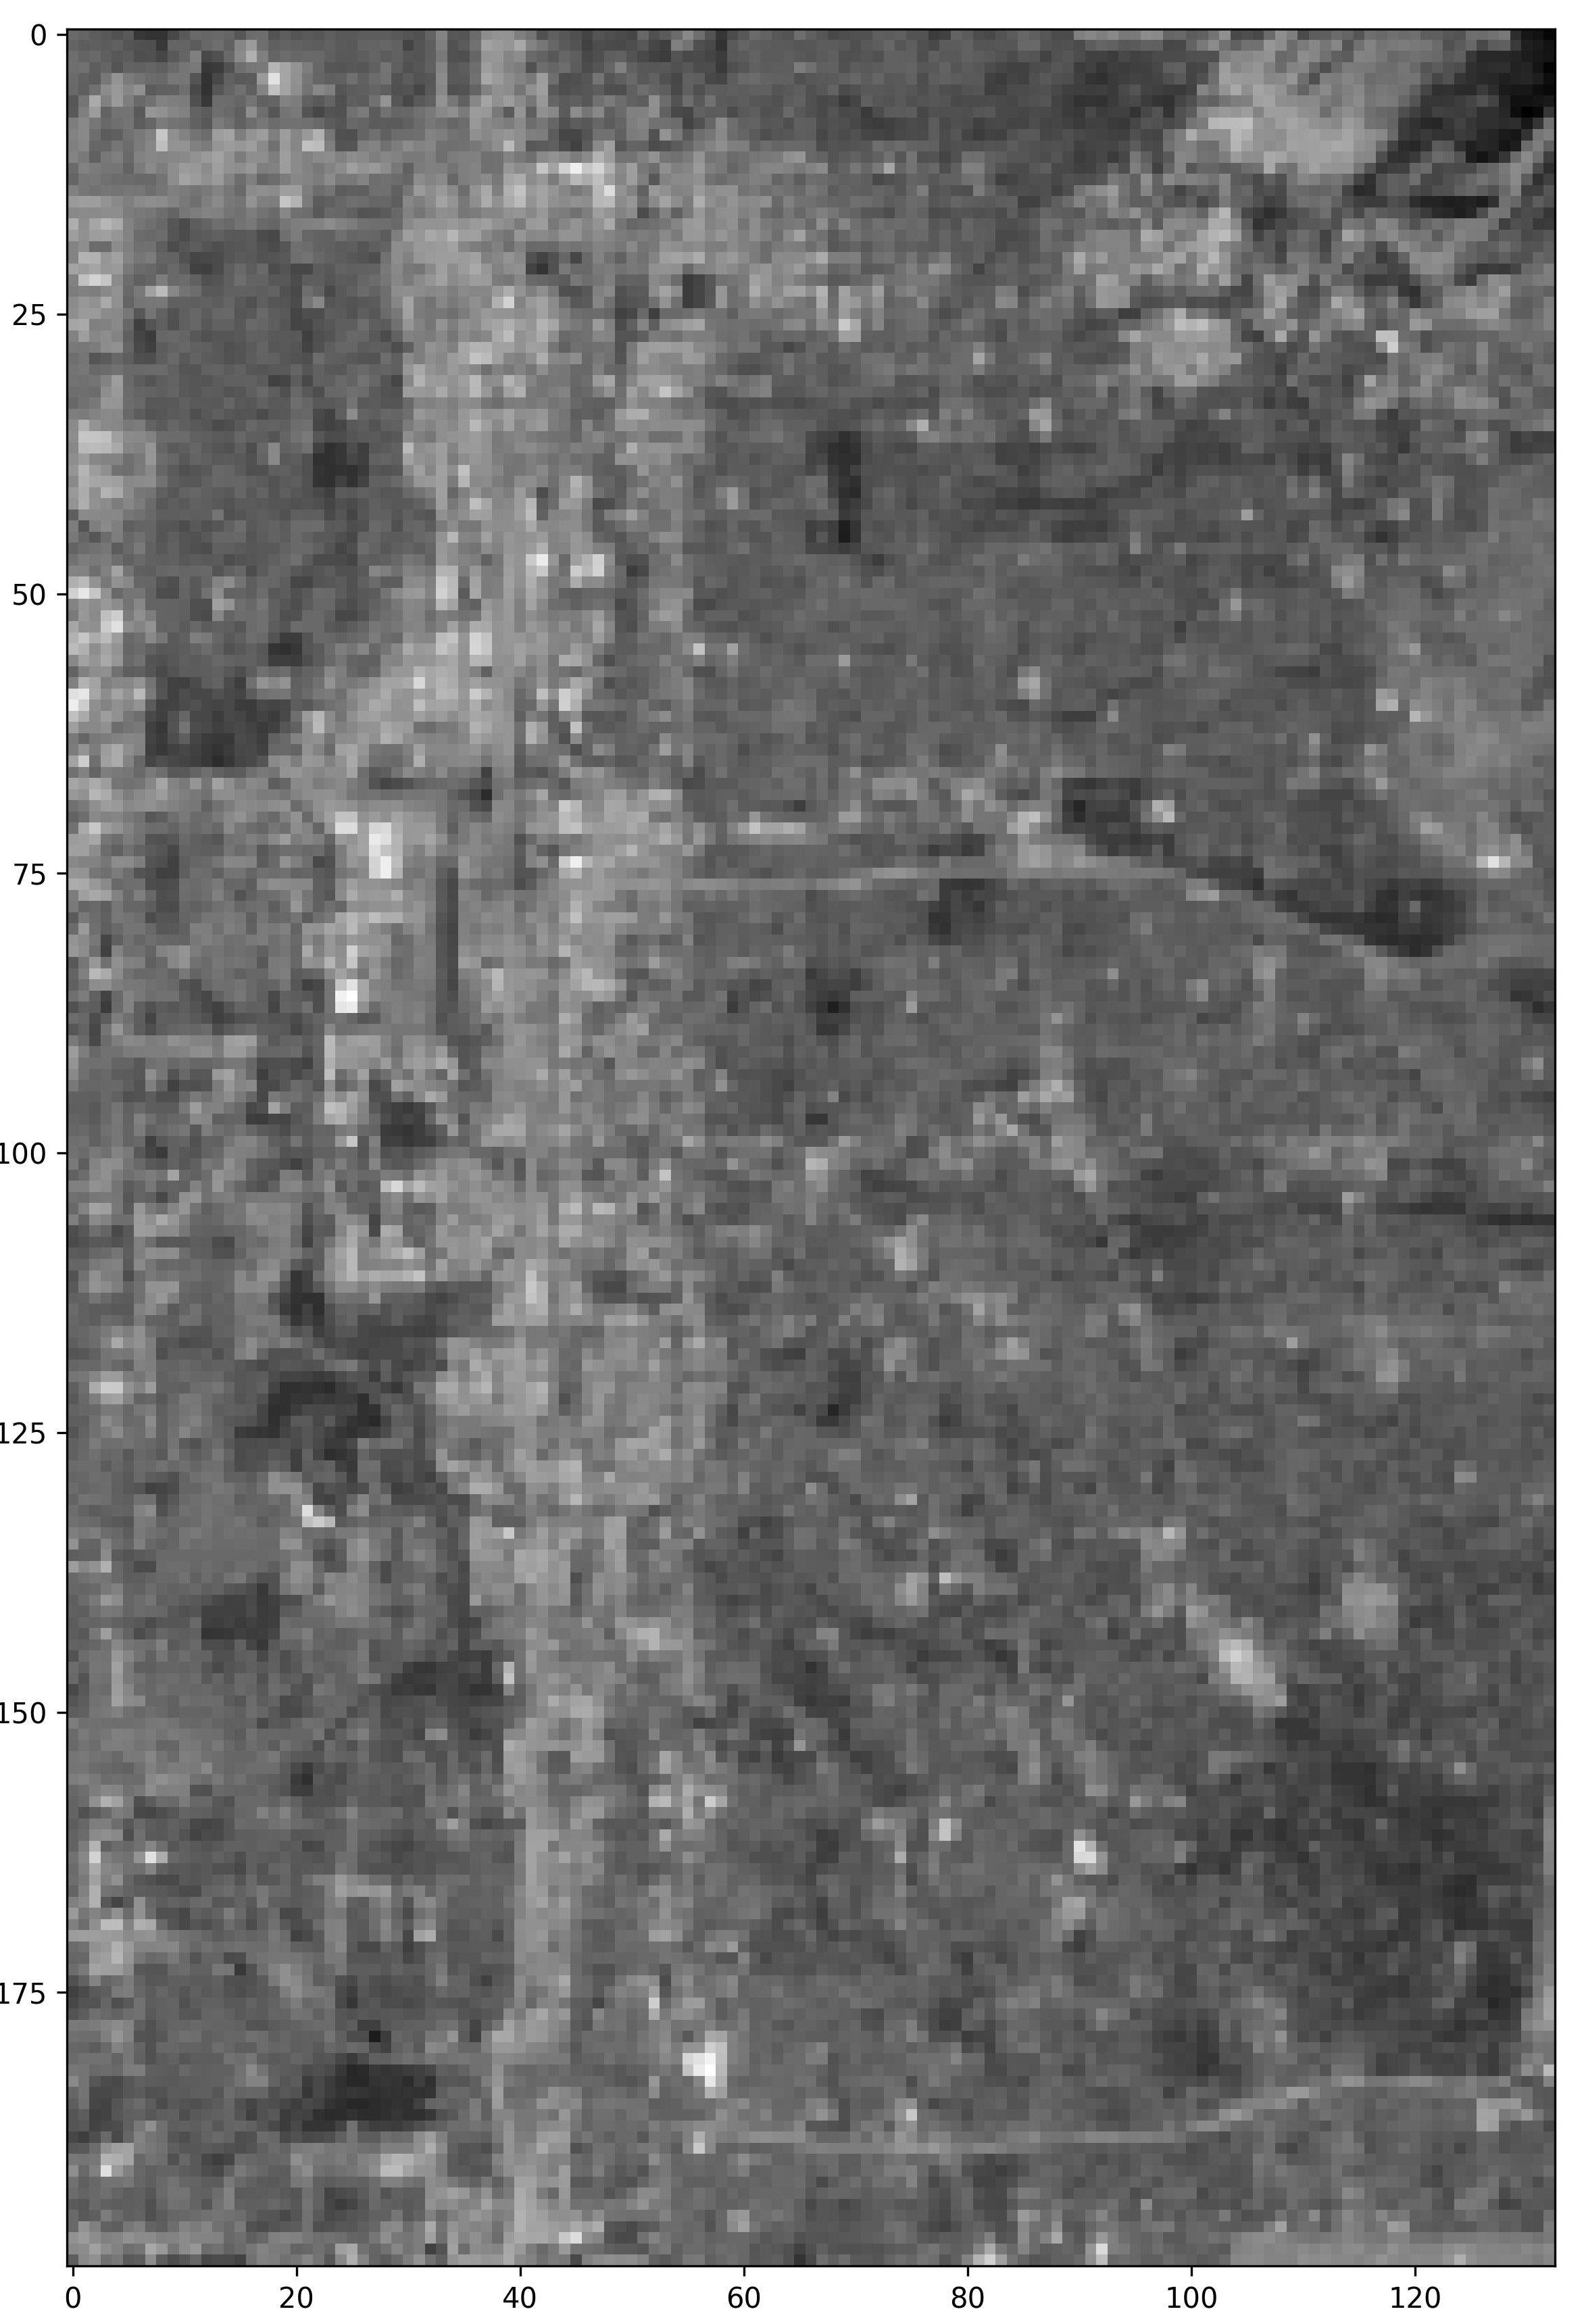
\includegraphics{images/plots/aerial_cities/1.jpg}

}

\subcaption{Salt Lake City, UT}

\end{figure}%

\end{minipage}%
%
\begin{minipage}{0.33\linewidth}

\begin{figure}[H]

{\centering 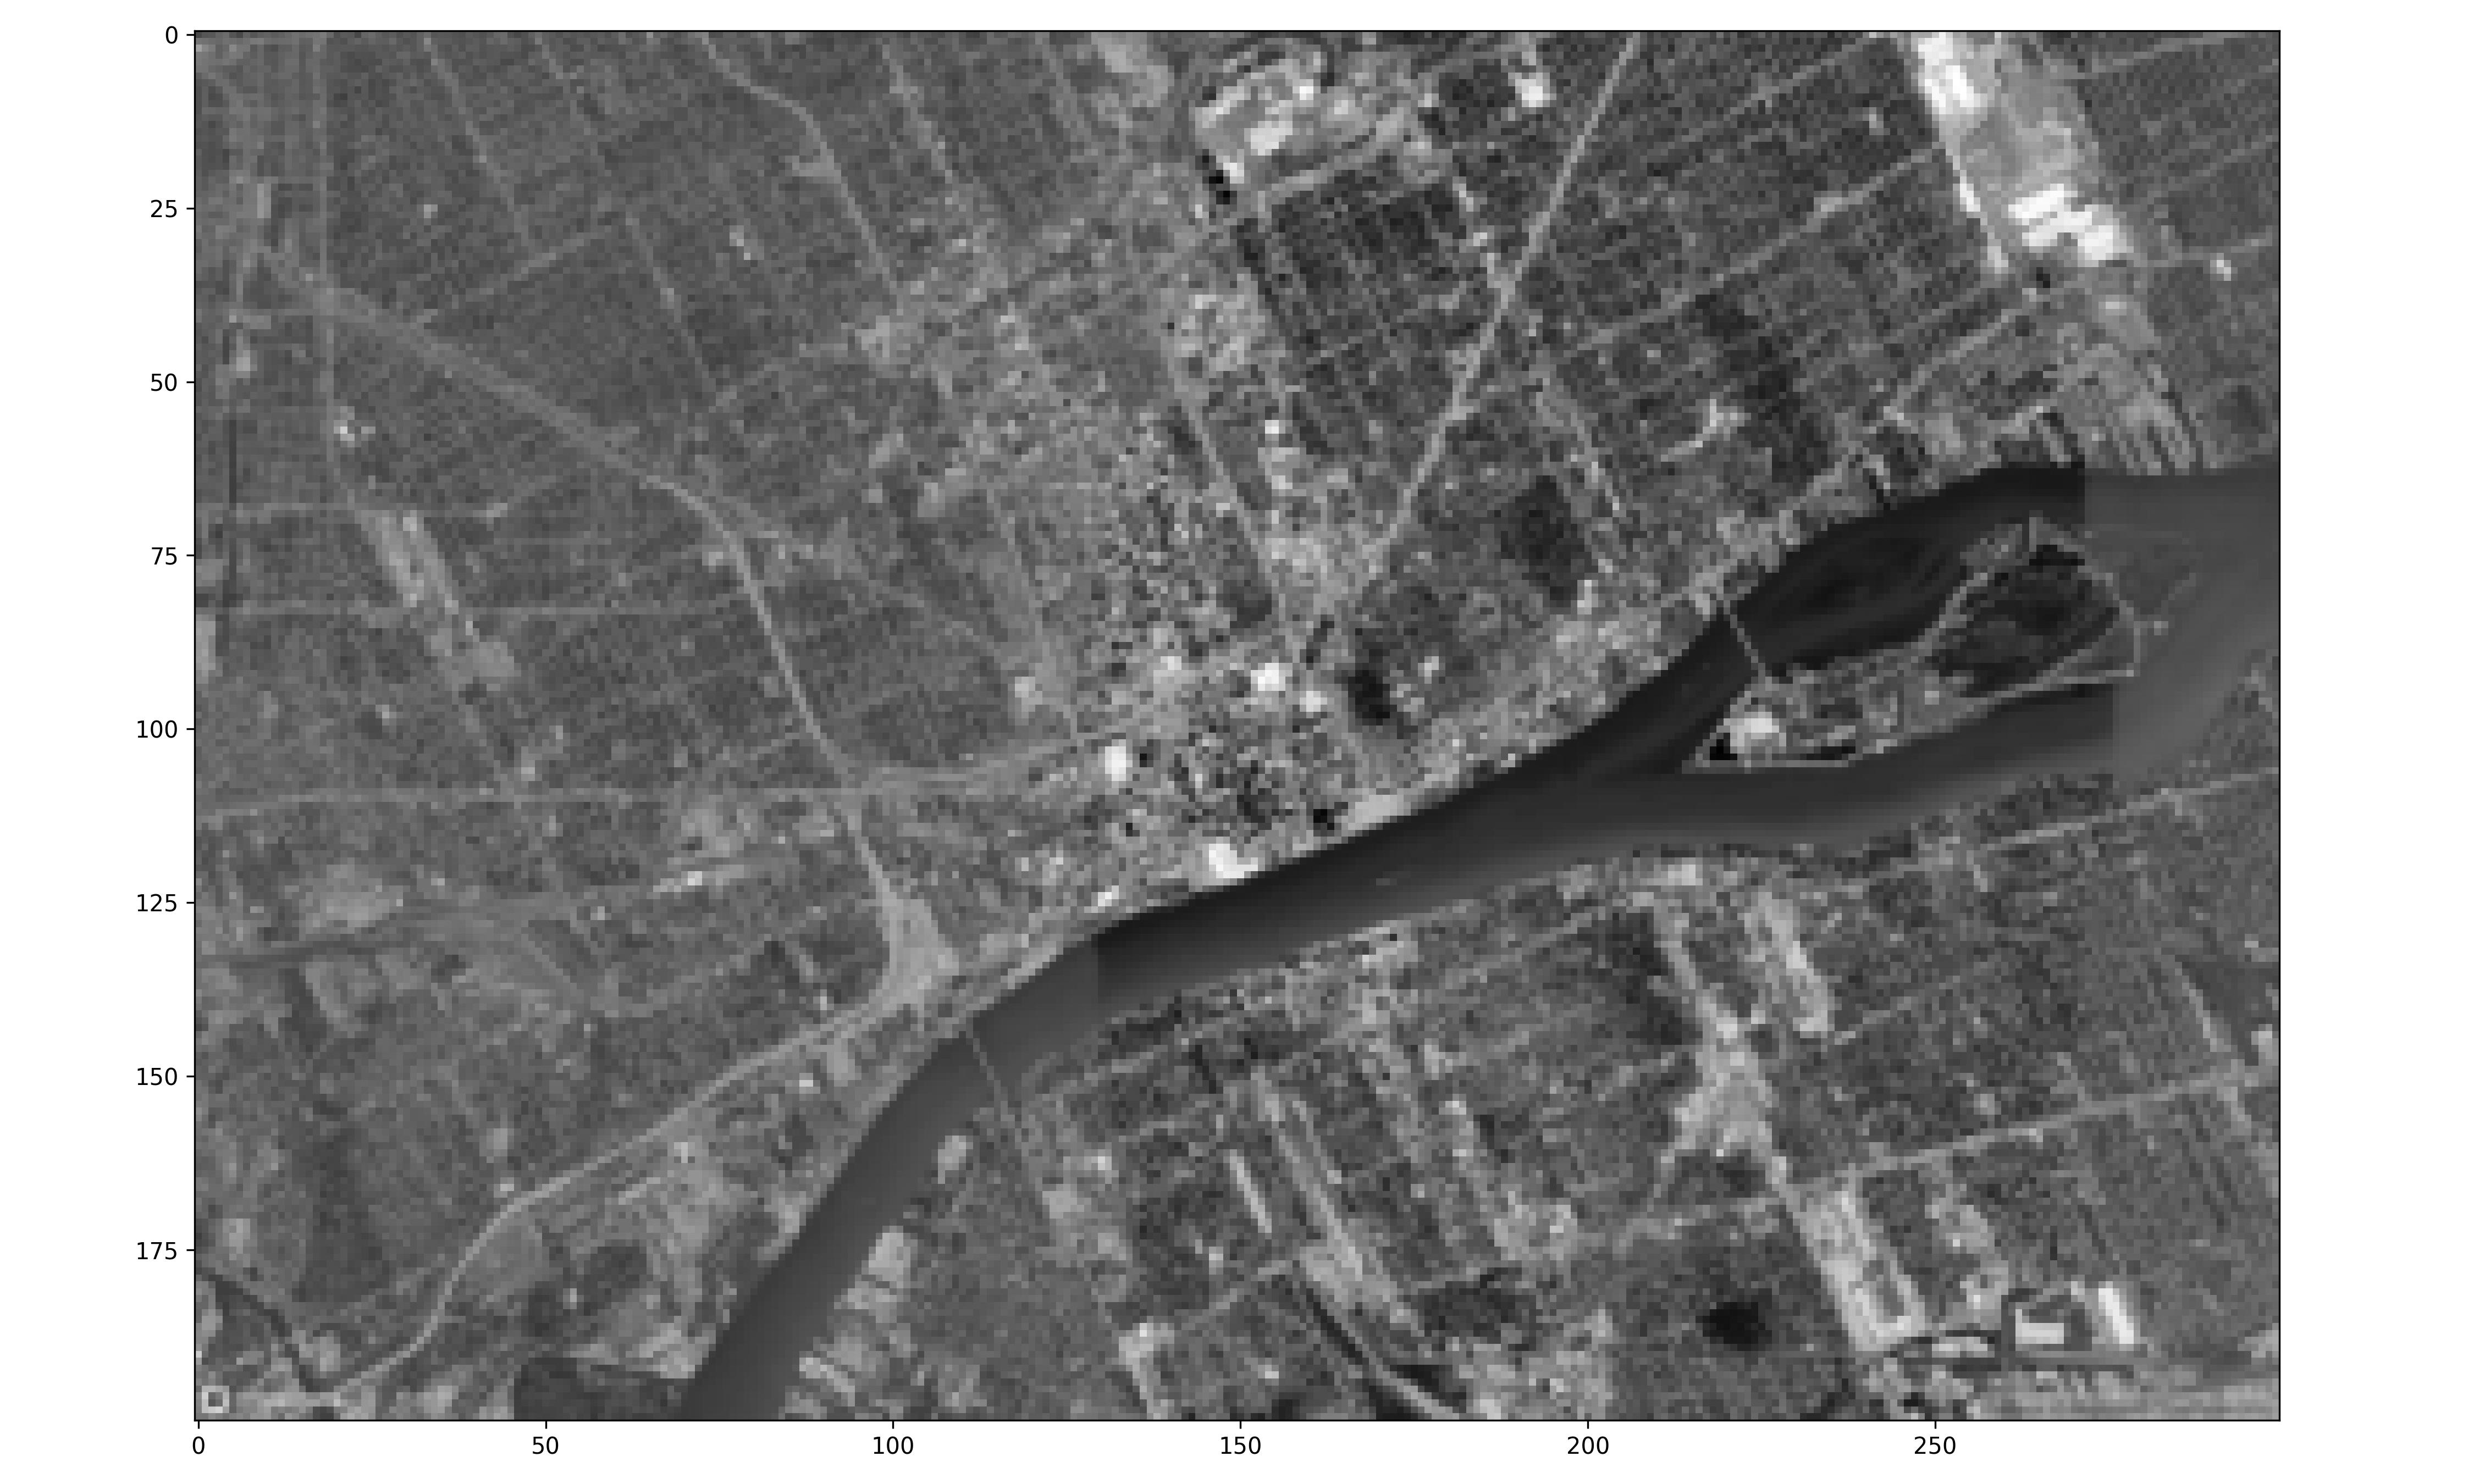
\includegraphics{images/plots/aerial_cities/2.jpg}

}

\subcaption{Detroit, MI}

\end{figure}%

\end{minipage}%

\caption{\label{fig-city-images}Aerial Cityscape Images Rescaled and
Converted to Greyscale}

\end{figure}%

\section{Build Data Frames for Each Aerial
Cityscape}\label{build-data-frames-for-each-aerial-cityscape}

\begin{Shaded}
\begin{Highlighting}[]
\CommentTok{\# San Francisco DF of gradient magnitudes and angles}
\NormalTok{mag\_sf }\OperatorTok{=}\NormalTok{ np.array(mag\_list[}\DecValTok{0}\NormalTok{])}
\NormalTok{theta\_sf }\OperatorTok{=}\NormalTok{ np.array(theta\_list[}\DecValTok{0}\NormalTok{])}

\CommentTok{\# Salt Lake City DF of gradient magnitudes and angles}
\NormalTok{mag\_salt\_lake }\OperatorTok{=}\NormalTok{ np.array(mag\_list[}\DecValTok{1}\NormalTok{])}
\NormalTok{theta\_salt\_lake }\OperatorTok{=}\NormalTok{ np.array(theta\_list[}\DecValTok{1}\NormalTok{])}

\CommentTok{\# Detorit DF of gradient magnitudes and angles}
\NormalTok{mag\_detroit }\OperatorTok{=}\NormalTok{ np.array(mag\_list[}\DecValTok{2}\NormalTok{])}
\NormalTok{theta\_detroit }\OperatorTok{=}\NormalTok{ np.array(theta\_list[}\DecValTok{2}\NormalTok{])}
\end{Highlighting}
\end{Shaded}

\section{Extract Gradient Magnitudes and Angles from each Aerial
Cityscape}\label{extract-gradient-magnitudes-and-angles-from-each-aerial-cityscape}

\begin{Shaded}
\begin{Highlighting}[]
\CommentTok{\# Save gradient magnitudes of San Francisco in image form}

\CommentTok{\# plt.figure(figsize=(15, 8))}
\CommentTok{\# \#plt.title(\textquotesingle{}San Francisco, CA Gradient Magnitudes\textquotesingle{})}
\CommentTok{\# plt.imshow(mag\_list[0], cmap="gray")}
\CommentTok{\# plt.axis("on")}
\CommentTok{\# \#plt.show()}
\CommentTok{\# plt.tight\_layout()}
\CommentTok{\# plt.savefig("images/plots/aerial\_cities/sf\_mag.png", dpi=300)}
\end{Highlighting}
\end{Shaded}

\begin{Shaded}
\begin{Highlighting}[]
\CommentTok{\# Save gradient magnitudes of Salt Lake City in image form}

\CommentTok{\# plt.figure(figsize=(8, 15))}
\CommentTok{\# \#plt.title(\textquotesingle{}Salt Lake City, UT Gradient Magnitudes\textquotesingle{})}
\CommentTok{\# plt.imshow(mag\_list[1], cmap="gray")}
\CommentTok{\# plt.axis("on")}
\CommentTok{\# \#plt.show()}
\CommentTok{\# plt.tight\_layout()}
\CommentTok{\# plt.savefig("images/plots/aerial\_cities/salt\_lake\_mag.png", dpi=300)}
\end{Highlighting}
\end{Shaded}

\begin{Shaded}
\begin{Highlighting}[]
\CommentTok{\# Save gradient magnitudes of Detroit in image form}

\CommentTok{\# plt.figure(figsize=(15, 8))}
\CommentTok{\# \#plt.title(\textquotesingle{}Detroit, MI Gradient Magnitudes\textquotesingle{})}
\CommentTok{\# plt.imshow(mag\_list[2], cmap="gray")}
\CommentTok{\# plt.axis("on")}
\CommentTok{\# \#plt.show()}
\CommentTok{\# plt.tight\_layout()}
\CommentTok{\# plt.savefig("images/plots/aerial\_cities/detroit\_mag.png", dpi=300)}
\end{Highlighting}
\end{Shaded}

\begin{figure}

\begin{minipage}{0.33\linewidth}

\begin{figure}[H]

{\centering 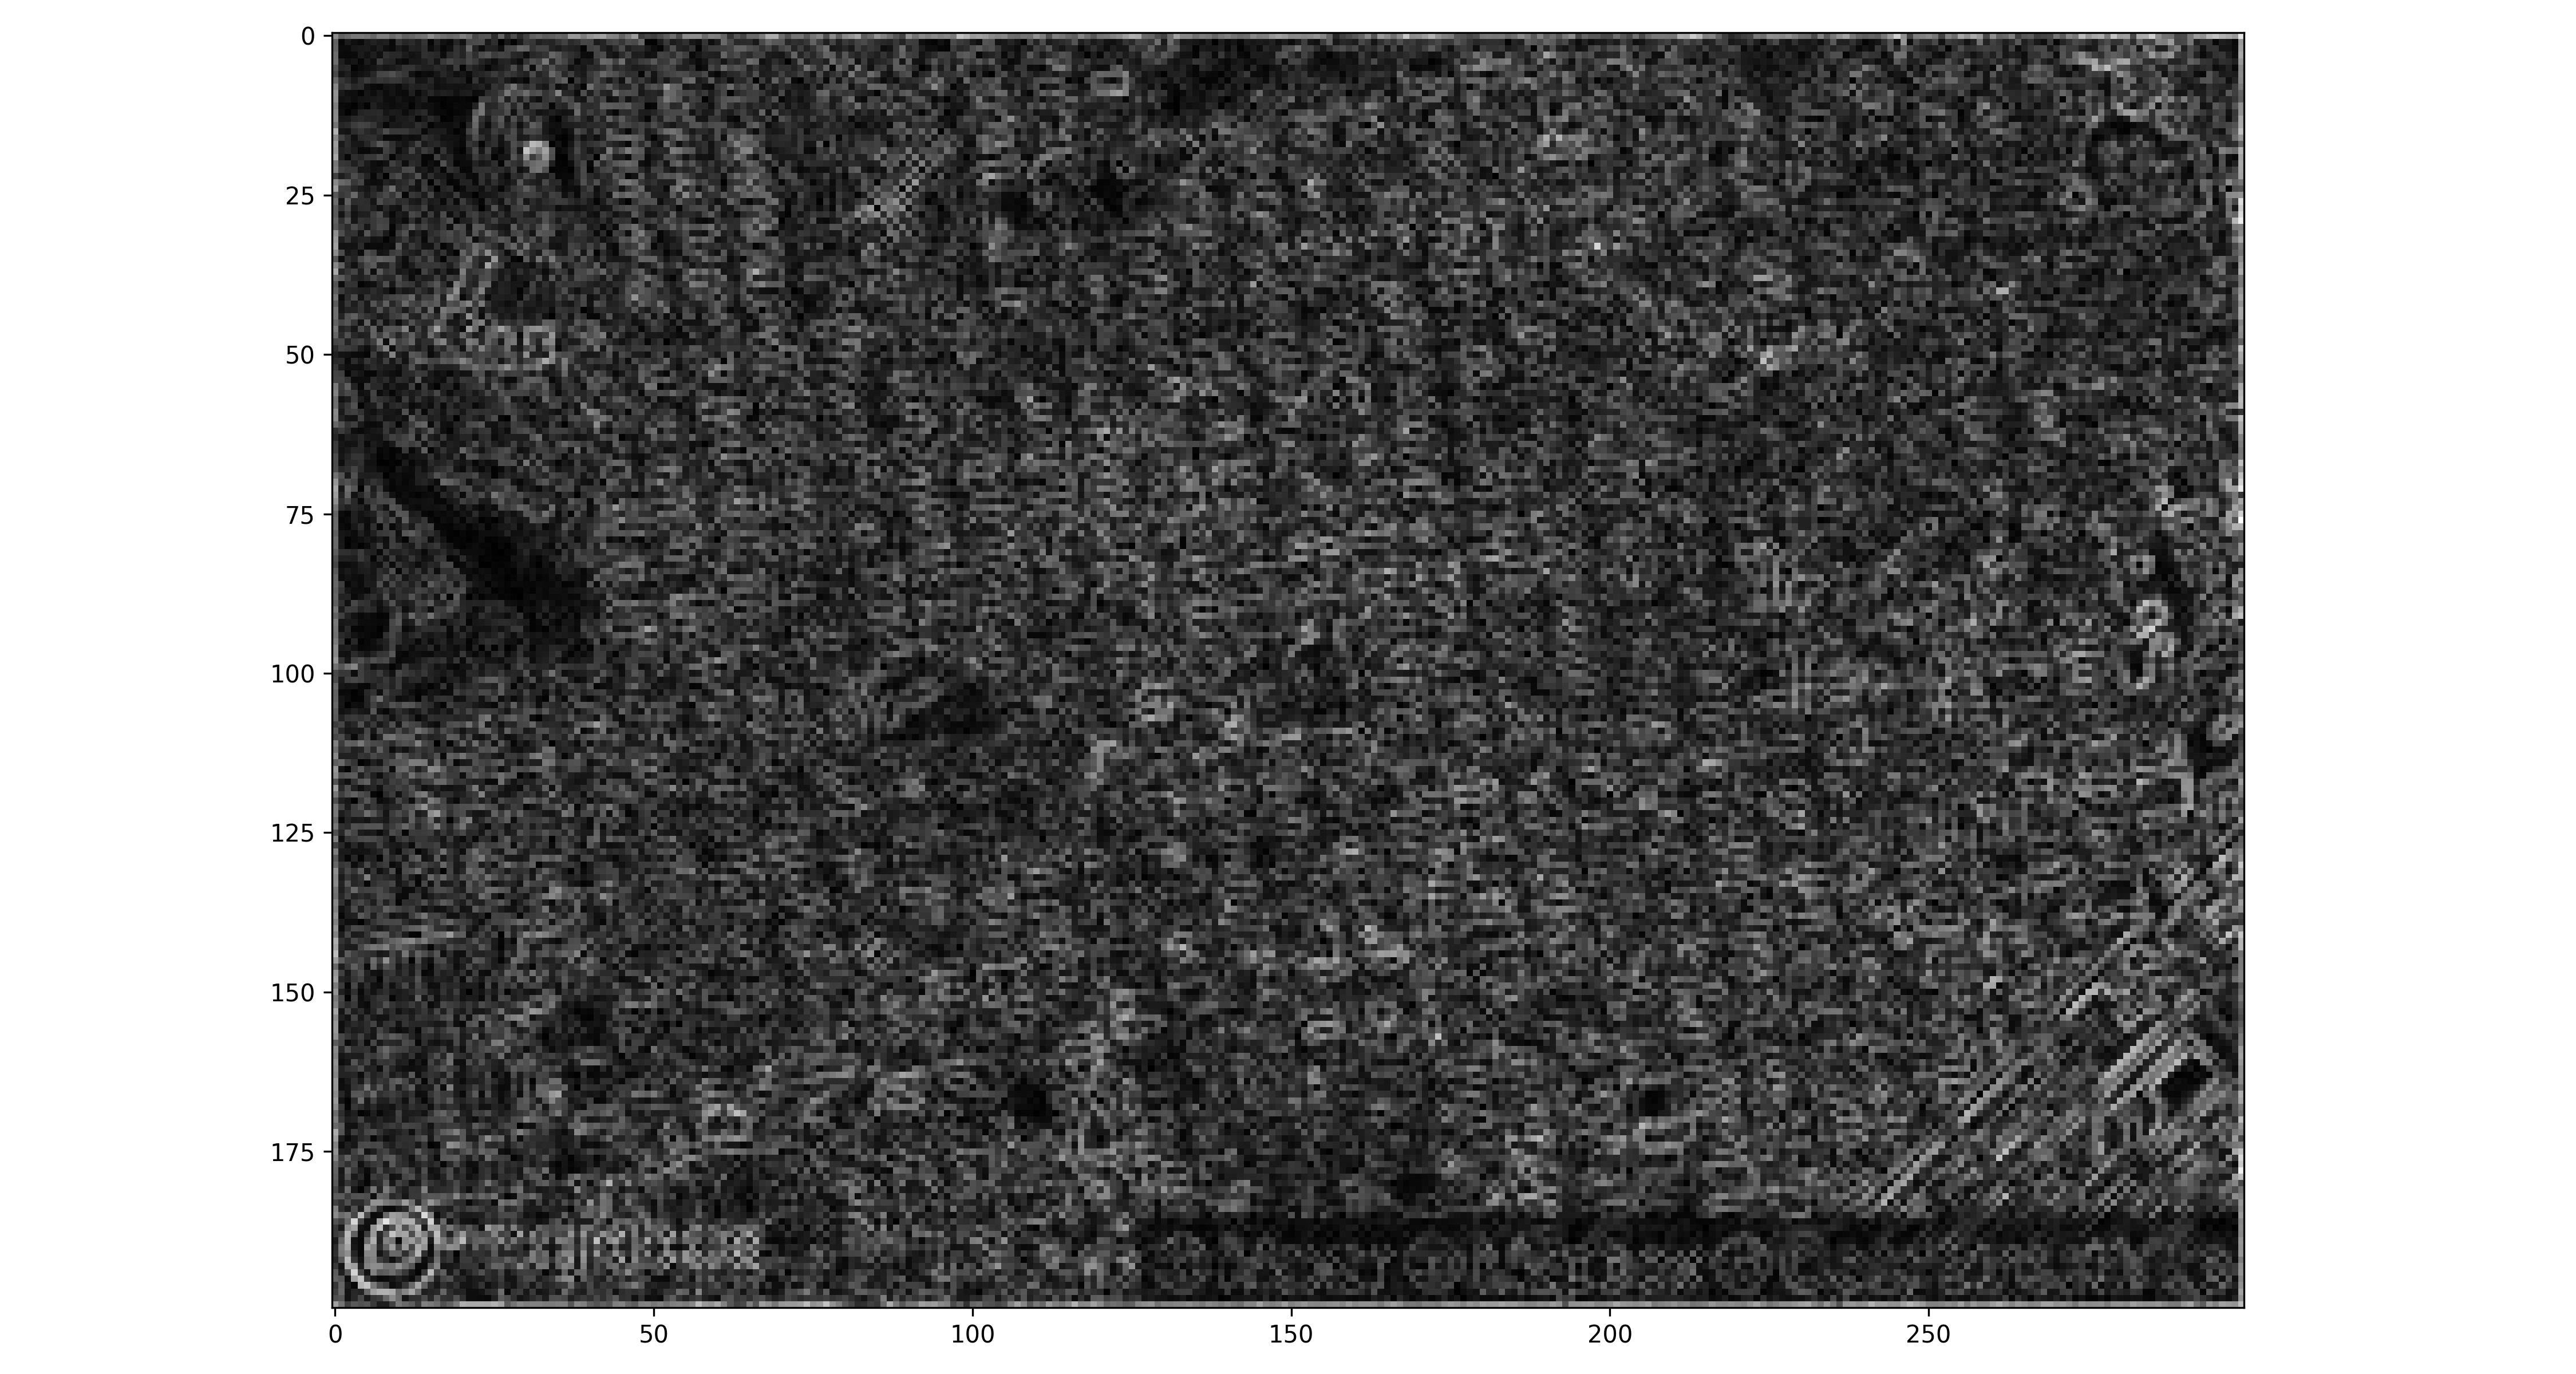
\includegraphics{images/plots/aerial_cities/sf_mag.png}

}

\subcaption{San Francisco, CA}

\end{figure}%

\end{minipage}%
%
\begin{minipage}{0.33\linewidth}

\begin{figure}[H]

{\centering 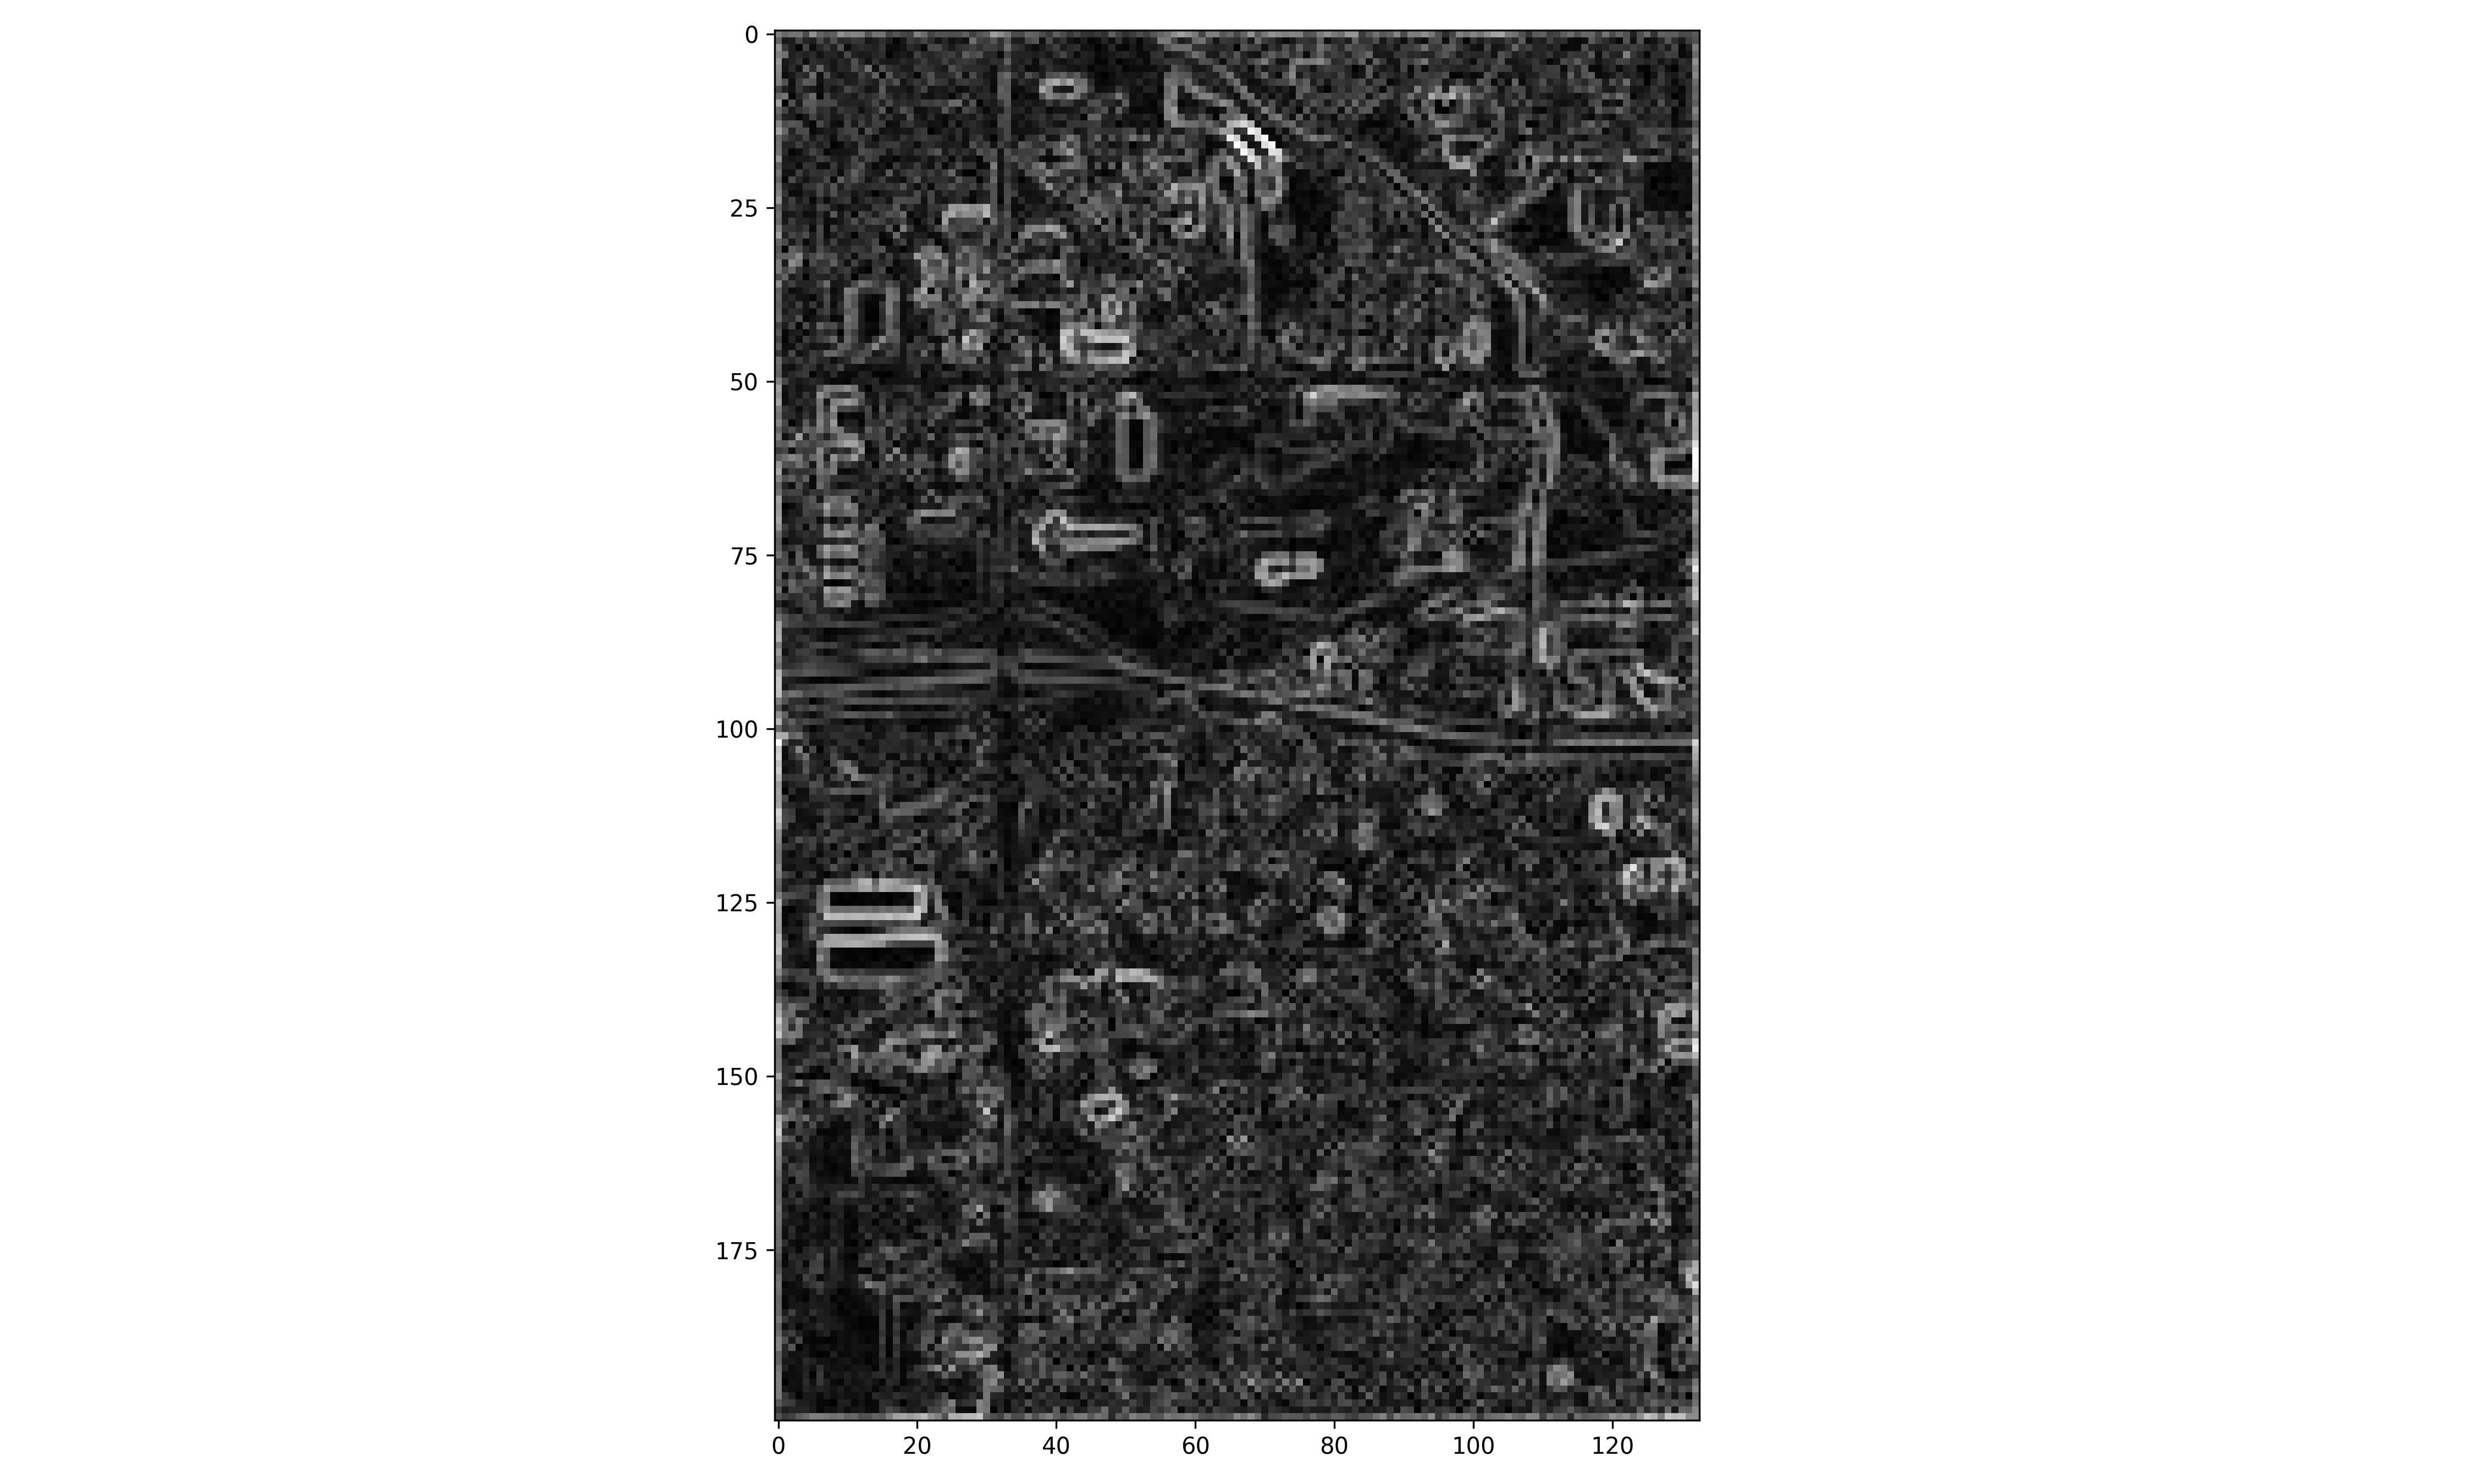
\includegraphics{images/plots/aerial_cities/salt_lake_mag.png}

}

\subcaption{Salt Lake City, UT}

\end{figure}%

\end{minipage}%
%
\begin{minipage}{0.33\linewidth}

\begin{figure}[H]

{\centering 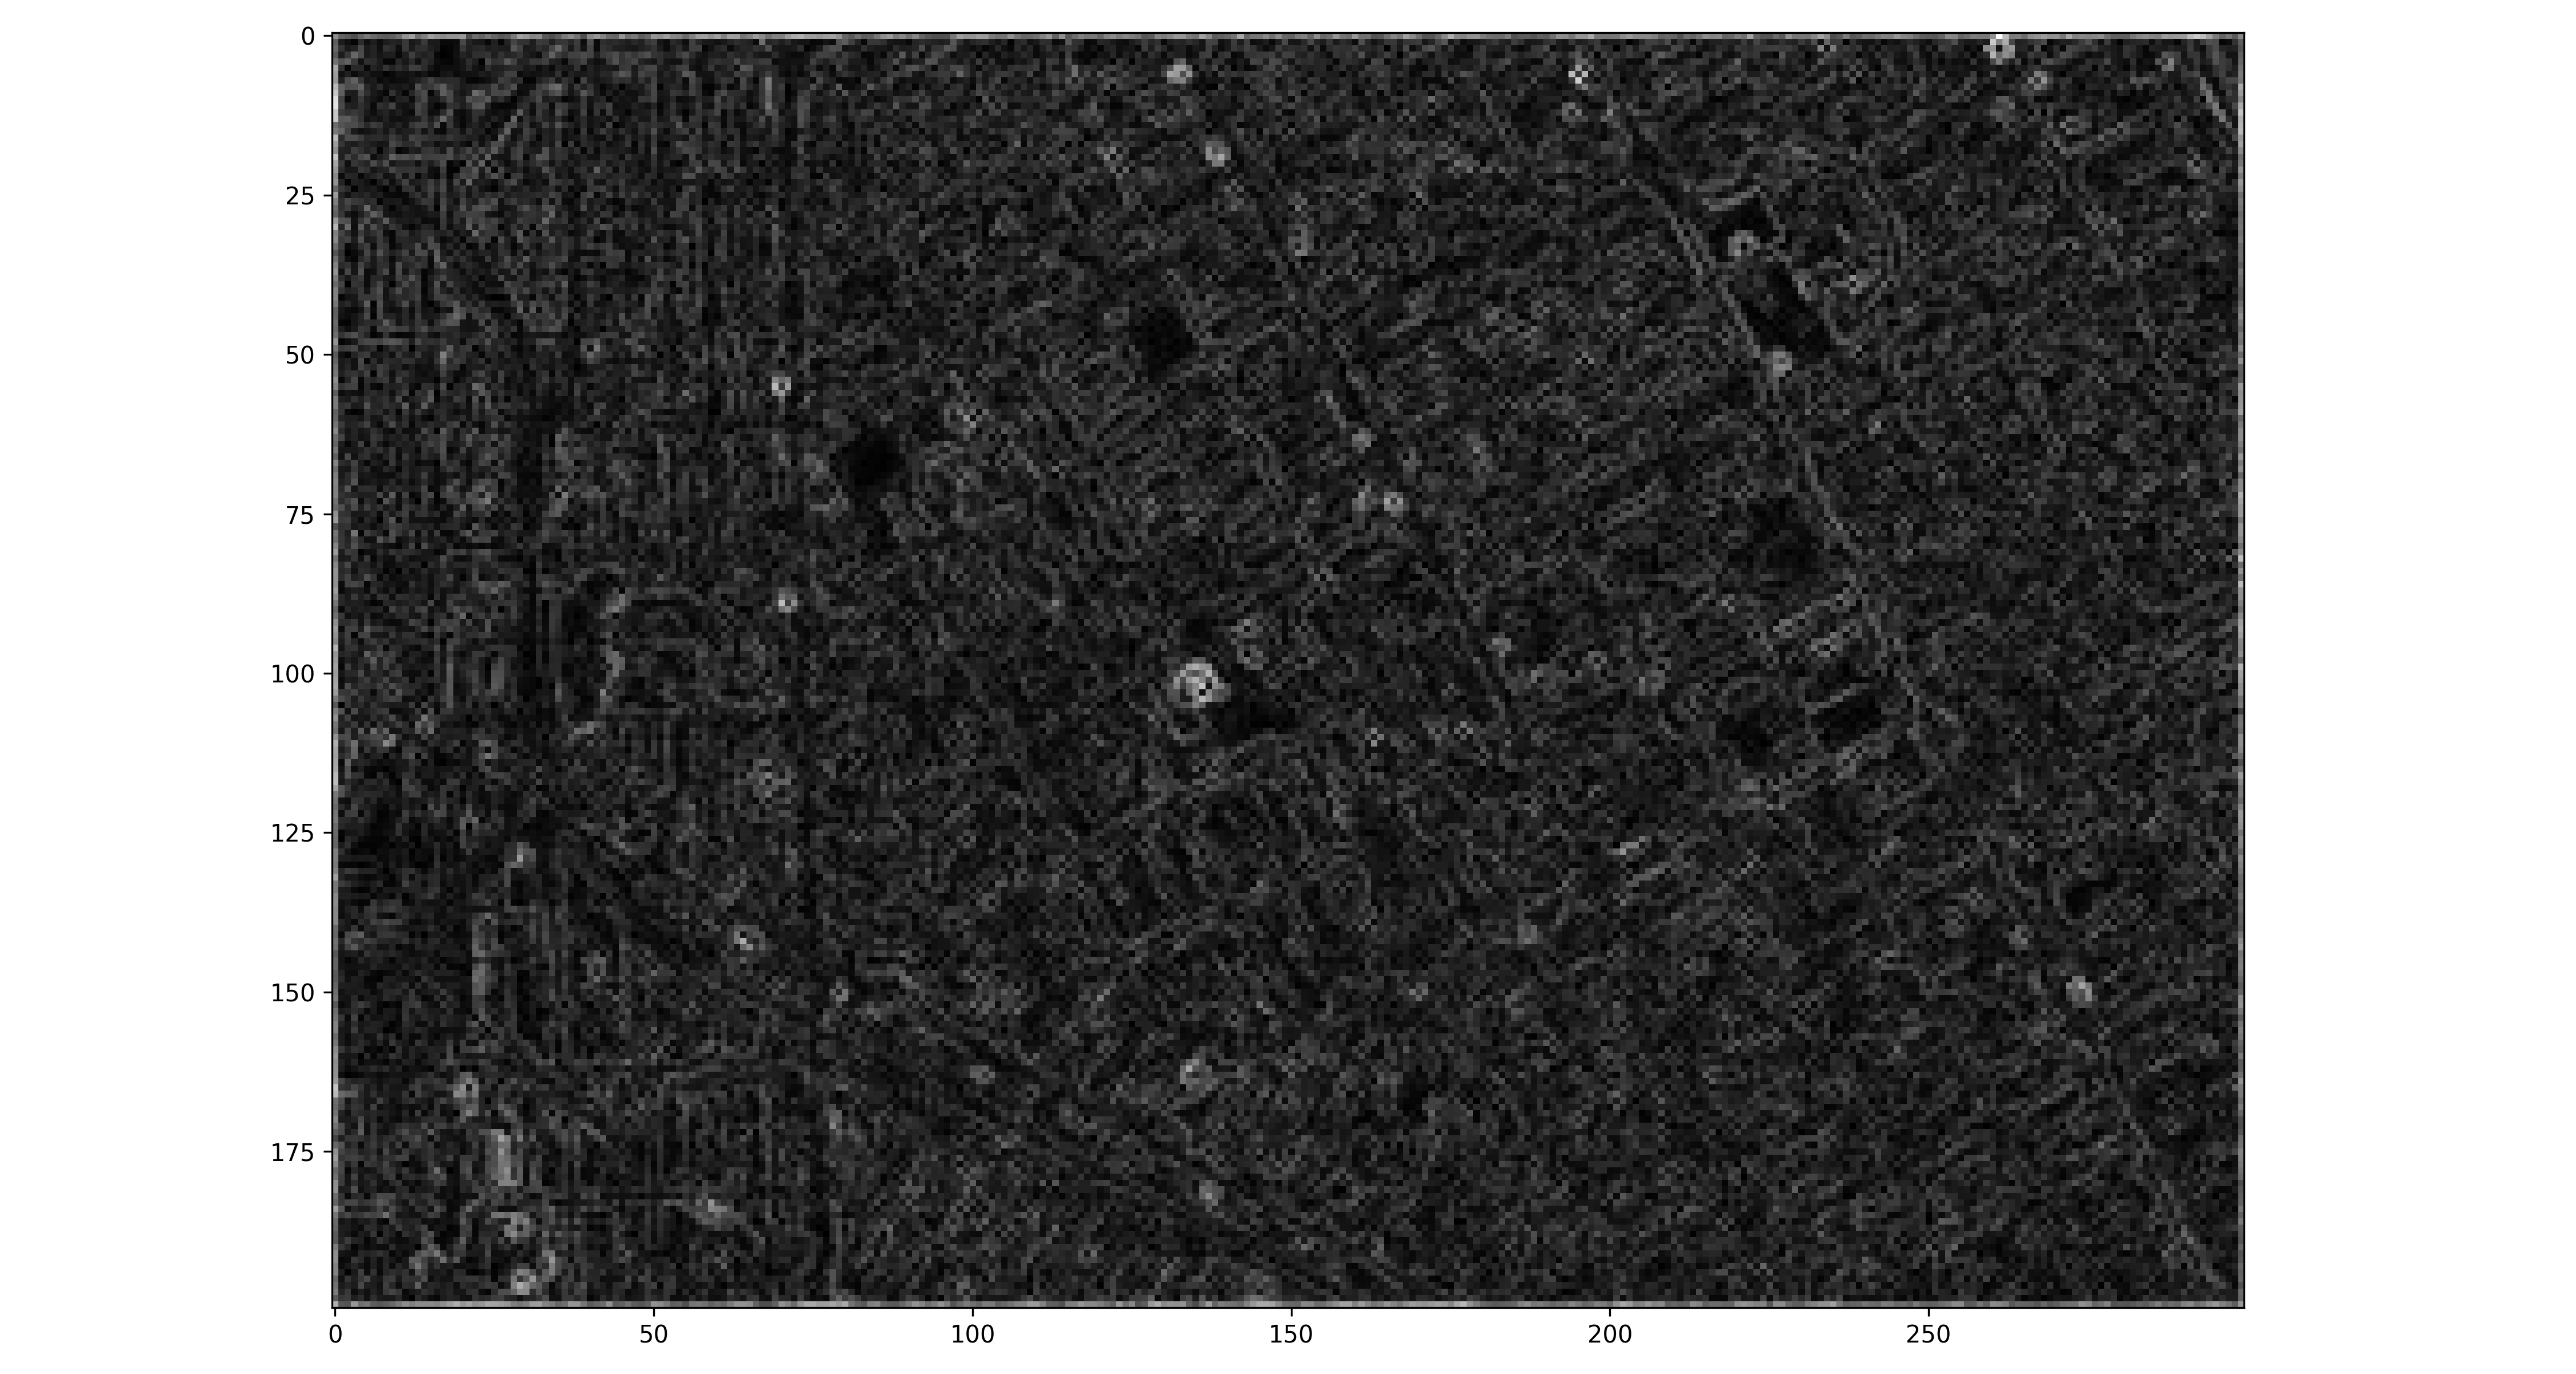
\includegraphics{images/plots/aerial_cities/detroit_mag.png}

}

\subcaption{Detroit, MI}

\end{figure}%

\end{minipage}%

\caption{\label{fig-city-mags}Aerial Cityscape Magnitudes}

\end{figure}%

\section{Create Data Frame for Each
Image}\label{create-data-frame-for-each-image}

\begin{Shaded}
\begin{Highlighting}[]
\CommentTok{\# San Francisco DF}
\NormalTok{sf\_hog\_df }\OtherTok{\textless{}{-}} \FunctionTok{data.frame}\NormalTok{(}\AttributeTok{mag =} \FunctionTok{as.vector}\NormalTok{(py}\SpecialCharTok{$}\NormalTok{mag\_sf),}
                              \AttributeTok{theta =} \FunctionTok{as.vector}\NormalTok{((py}\SpecialCharTok{$}\NormalTok{theta\_sf))) }\SpecialCharTok{\%\textgreater{}\%}
  \FunctionTok{mutate}\NormalTok{(}\AttributeTok{radian =}\NormalTok{ theta}\SpecialCharTok{*}\NormalTok{(pi}\SpecialCharTok{/}\DecValTok{180}\NormalTok{))}
\end{Highlighting}
\end{Shaded}

\begin{Shaded}
\begin{Highlighting}[]
\CommentTok{\# Salt Lake City DF}
\NormalTok{salt\_lake\_hog\_df }\OtherTok{\textless{}{-}} \FunctionTok{data.frame}\NormalTok{(}\AttributeTok{mag =} \FunctionTok{as.vector}\NormalTok{(py}\SpecialCharTok{$}\NormalTok{mag\_salt\_lake),}
                              \AttributeTok{theta =} \FunctionTok{as.vector}\NormalTok{((py}\SpecialCharTok{$}\NormalTok{theta\_salt\_lake))) }\SpecialCharTok{\%\textgreater{}\%}
  \FunctionTok{mutate}\NormalTok{(}\AttributeTok{radian =}\NormalTok{ theta}\SpecialCharTok{*}\NormalTok{(pi}\SpecialCharTok{/}\DecValTok{180}\NormalTok{))}
\end{Highlighting}
\end{Shaded}

\begin{Shaded}
\begin{Highlighting}[]
\CommentTok{\# Detroit DF}
\NormalTok{detroit\_hog\_df }\OtherTok{\textless{}{-}} \FunctionTok{data.frame}\NormalTok{(}\AttributeTok{mag =} \FunctionTok{as.vector}\NormalTok{(py}\SpecialCharTok{$}\NormalTok{mag\_detroit),}
                              \AttributeTok{theta =} \FunctionTok{as.vector}\NormalTok{((py}\SpecialCharTok{$}\NormalTok{theta\_detroit))) }\SpecialCharTok{\%\textgreater{}\%}
  \FunctionTok{mutate}\NormalTok{(}\AttributeTok{radian =}\NormalTok{ theta}\SpecialCharTok{*}\NormalTok{(pi}\SpecialCharTok{/}\DecValTok{180}\NormalTok{))}
\end{Highlighting}
\end{Shaded}

\begin{Shaded}
\begin{Highlighting}[]
\CommentTok{\# List of all Data frames}
\NormalTok{standard\_df\_list }\OtherTok{=} \FunctionTok{list}\NormalTok{(sf\_hog\_df,}
\NormalTok{                        salt\_lake\_hog\_df, }
\NormalTok{                        detroit\_hog\_df)}
\end{Highlighting}
\end{Shaded}

\section{Create Histograms of Gradient Magnitudes and Angles for Aerial
Cityscapes}\label{create-histograms-of-gradient-magnitudes-and-angles-for-aerial-cityscapes}

\begin{Shaded}
\begin{Highlighting}[]
\CommentTok{\# SF histogram of gradient mags}
\NormalTok{sf\_histogram\_mag\_plot }\OtherTok{\textless{}{-}}
  \FunctionTok{ggplot}\NormalTok{(standard\_df\_list[[}\DecValTok{1}\NormalTok{]], }
         \FunctionTok{aes}\NormalTok{(}\AttributeTok{x =}\NormalTok{ mag)) }\SpecialCharTok{+}
  \FunctionTok{geom\_histogram}\NormalTok{(}\AttributeTok{colour =} \StringTok{"black"}\NormalTok{, }\AttributeTok{fill =} \StringTok{"lightblue"}\NormalTok{) }\SpecialCharTok{+}
  \FunctionTok{scale\_x\_continuous}\NormalTok{() }\SpecialCharTok{+} 
  \FunctionTok{labs}\NormalTok{(}\AttributeTok{x =} \StringTok{"Gradient Magnitude"}\NormalTok{, }
       \AttributeTok{y =} \StringTok{"Count"}\NormalTok{, }
       \AttributeTok{title =} \StringTok{"San Francisco Cityscape Image Histogram of Gradient Magnitudes"}
\NormalTok{       ) }\SpecialCharTok{+}
  \FunctionTok{theme\_minimal}\NormalTok{() }\SpecialCharTok{+}
  \FunctionTok{theme}\NormalTok{(}\AttributeTok{plot.title =} \FunctionTok{element\_text}\NormalTok{(}\AttributeTok{hjust =} \FloatTok{0.5}\NormalTok{))}

\CommentTok{\# sf mag filter level}
\NormalTok{sf\_mag\_filter }\OtherTok{\textless{}{-}} \FloatTok{0.4}

\CommentTok{\# save image}
\FunctionTok{ggsave}\NormalTok{(}\StringTok{"images/plots/aerial\_cities/sf\_histogram\_mag\_plot.jpg"}\NormalTok{, sf\_histogram\_mag\_plot, }\AttributeTok{width =} \DecValTok{6}\NormalTok{, }\AttributeTok{height =} \DecValTok{4}\NormalTok{, }\AttributeTok{dpi =} \DecValTok{300}\NormalTok{)}
\end{Highlighting}
\end{Shaded}

\begin{Shaded}
\begin{Highlighting}[]
\CommentTok{\# SF histogram of gradient angles}
\NormalTok{sf\_histogram\_theta\_plot }\OtherTok{\textless{}{-}}
  \FunctionTok{ggplot}\NormalTok{(standard\_df\_list[[}\DecValTok{1}\NormalTok{]], }
         \FunctionTok{aes}\NormalTok{(}\AttributeTok{x =}\NormalTok{ theta)) }\SpecialCharTok{+}
  \FunctionTok{geom\_histogram}\NormalTok{(}\AttributeTok{colour =} \StringTok{"black"}\NormalTok{, }\AttributeTok{fill =} \StringTok{"lightblue"}\NormalTok{) }\SpecialCharTok{+}
  \FunctionTok{scale\_x\_continuous}\NormalTok{() }\SpecialCharTok{+} 
  \FunctionTok{labs}\NormalTok{(}\AttributeTok{x =} \StringTok{"Gradient Angle"}\NormalTok{, }
       \AttributeTok{y =} \StringTok{"Count"}\NormalTok{, }
       \AttributeTok{title =} \StringTok{"San Francisco Cityscape Image Histogram of Gradient Angles"}
\NormalTok{       ) }\SpecialCharTok{+}
  \FunctionTok{theme\_minimal}\NormalTok{() }\SpecialCharTok{+}
  \FunctionTok{theme}\NormalTok{(}\AttributeTok{plot.title =} \FunctionTok{element\_text}\NormalTok{(}\AttributeTok{hjust =} \FloatTok{0.5}\NormalTok{))}

\CommentTok{\# save image}
\FunctionTok{ggsave}\NormalTok{(}\StringTok{"images/plots/aerial\_cities/sf\_histogram\_theta\_plot.jpg"}\NormalTok{, sf\_histogram\_theta\_plot, }\AttributeTok{width =} \DecValTok{6}\NormalTok{, }\AttributeTok{height =} \DecValTok{4}\NormalTok{, }\AttributeTok{dpi =} \DecValTok{300}\NormalTok{)}
\end{Highlighting}
\end{Shaded}

\begin{Shaded}
\begin{Highlighting}[]
\CommentTok{\# slc histogram of gradient mags}
\NormalTok{salt\_lake\_histogram\_mag\_plot }\OtherTok{\textless{}{-}}
  \FunctionTok{ggplot}\NormalTok{(standard\_df\_list[[}\DecValTok{2}\NormalTok{]], }
         \FunctionTok{aes}\NormalTok{(}\AttributeTok{x =}\NormalTok{ mag)) }\SpecialCharTok{+}
  \FunctionTok{geom\_histogram}\NormalTok{(}\AttributeTok{colour =} \StringTok{"black"}\NormalTok{, }\AttributeTok{fill =} \StringTok{"lightblue"}\NormalTok{) }\SpecialCharTok{+}
  \FunctionTok{scale\_x\_continuous}\NormalTok{() }\SpecialCharTok{+} 
  \FunctionTok{labs}\NormalTok{(}\AttributeTok{x =} \StringTok{"Gradient Magnitude"}\NormalTok{, }
       \AttributeTok{y =} \StringTok{"Count"}\NormalTok{, }
       \AttributeTok{title =} \StringTok{"Salt Lake City Image Histogram of Gradient Magnitudes"}
\NormalTok{       ) }\SpecialCharTok{+}
  \FunctionTok{theme\_minimal}\NormalTok{() }\SpecialCharTok{+}
  \FunctionTok{theme}\NormalTok{(}\AttributeTok{plot.title =} \FunctionTok{element\_text}\NormalTok{(}\AttributeTok{hjust =} \FloatTok{0.5}\NormalTok{))}

\CommentTok{\# SLC mag filter level}
\NormalTok{salt\_lake\_mag\_filter }\OtherTok{\textless{}{-}} \FloatTok{0.12}

\CommentTok{\# save image}
\FunctionTok{ggsave}\NormalTok{(}\StringTok{"images/plots/aerial\_cities/salt\_lake\_histogram\_mag\_plot.jpg"}\NormalTok{, salt\_lake\_histogram\_mag\_plot, }\AttributeTok{width =} \DecValTok{6}\NormalTok{, }\AttributeTok{height =} \DecValTok{4}\NormalTok{, }\AttributeTok{dpi =} \DecValTok{300}\NormalTok{)}
\end{Highlighting}
\end{Shaded}

\begin{Shaded}
\begin{Highlighting}[]
\CommentTok{\# slc histogram of gradient angles}
\NormalTok{salt\_lake\_histogram\_theta\_plot }\OtherTok{\textless{}{-}}
  \FunctionTok{ggplot}\NormalTok{(standard\_df\_list[[}\DecValTok{2}\NormalTok{]], }
         \FunctionTok{aes}\NormalTok{(}\AttributeTok{x =}\NormalTok{ theta)) }\SpecialCharTok{+}
  \FunctionTok{geom\_histogram}\NormalTok{(}\AttributeTok{colour =} \StringTok{"black"}\NormalTok{, }\AttributeTok{fill =} \StringTok{"lightblue"}\NormalTok{) }\SpecialCharTok{+}
  \FunctionTok{scale\_x\_continuous}\NormalTok{() }\SpecialCharTok{+} 
  \FunctionTok{labs}\NormalTok{(}\AttributeTok{x =} \StringTok{"Gradient Angle"}\NormalTok{, }
       \AttributeTok{y =} \StringTok{"Count"}\NormalTok{, }
       \AttributeTok{title =} \StringTok{"Salt Lake City Image Histogram of Gradient Angles"}
\NormalTok{       ) }\SpecialCharTok{+}
  \FunctionTok{theme\_minimal}\NormalTok{() }\SpecialCharTok{+}
  \FunctionTok{theme}\NormalTok{(}\AttributeTok{plot.title =} \FunctionTok{element\_text}\NormalTok{(}\AttributeTok{hjust =} \FloatTok{0.5}\NormalTok{))}

\CommentTok{\# save image}
\FunctionTok{ggsave}\NormalTok{(}\StringTok{"images/plots/aerial\_cities/salt\_lake\_histogram\_theta\_plot.jpg"}\NormalTok{, salt\_lake\_histogram\_theta\_plot, }\AttributeTok{width =} \DecValTok{6}\NormalTok{, }\AttributeTok{height =} \DecValTok{4}\NormalTok{, }\AttributeTok{dpi =} \DecValTok{300}\NormalTok{)}
\end{Highlighting}
\end{Shaded}

\begin{Shaded}
\begin{Highlighting}[]
\CommentTok{\# Detroit histogram of gradient mags}
\NormalTok{detroit\_histogram\_mag\_plot }\OtherTok{\textless{}{-}}
  \FunctionTok{ggplot}\NormalTok{(standard\_df\_list[[}\DecValTok{3}\NormalTok{]], }
         \FunctionTok{aes}\NormalTok{(}\AttributeTok{x =}\NormalTok{ mag)) }\SpecialCharTok{+}
  \FunctionTok{geom\_histogram}\NormalTok{(}\AttributeTok{colour =} \StringTok{"black"}\NormalTok{, }\AttributeTok{fill =} \StringTok{"lightblue"}\NormalTok{) }\SpecialCharTok{+}
  \FunctionTok{scale\_x\_continuous}\NormalTok{() }\SpecialCharTok{+} 
  \FunctionTok{labs}\NormalTok{(}\AttributeTok{x =} \StringTok{"Gradient Magnitude"}\NormalTok{, }
       \AttributeTok{y =} \StringTok{"Count"}\NormalTok{, }
       \AttributeTok{title =} \StringTok{"Detroit Image Histogram of Gradient Magnitudes"}
\NormalTok{       ) }\SpecialCharTok{+}
  \FunctionTok{theme\_minimal}\NormalTok{() }\SpecialCharTok{+}
  \FunctionTok{theme}\NormalTok{(}\AttributeTok{plot.title =} \FunctionTok{element\_text}\NormalTok{(}\AttributeTok{hjust =} \FloatTok{0.5}\NormalTok{))}

\CommentTok{\# Detroit mag filter level}
\NormalTok{detroit\_mag\_filter }\OtherTok{\textless{}{-}} \FloatTok{0.15}

\FunctionTok{ggsave}\NormalTok{(}\StringTok{"images/plots/aerial\_cities/detroit\_histogram\_mag\_plot.jpg"}\NormalTok{, detroit\_histogram\_mag\_plot, }\AttributeTok{width =} \DecValTok{6}\NormalTok{, }\AttributeTok{height =} \DecValTok{4}\NormalTok{, }\AttributeTok{dpi =} \DecValTok{300}\NormalTok{)}
\end{Highlighting}
\end{Shaded}

\begin{Shaded}
\begin{Highlighting}[]
\CommentTok{\# Detroit histogram of gradient angles}
\NormalTok{detroit\_histogram\_theta\_plot }\OtherTok{\textless{}{-}}
  \FunctionTok{ggplot}\NormalTok{(standard\_df\_list[[}\DecValTok{3}\NormalTok{]], }
         \FunctionTok{aes}\NormalTok{(}\AttributeTok{x =}\NormalTok{ theta)) }\SpecialCharTok{+}
  \FunctionTok{geom\_histogram}\NormalTok{(}\AttributeTok{colour =} \StringTok{"black"}\NormalTok{, }\AttributeTok{fill =} \StringTok{"lightblue"}\NormalTok{) }\SpecialCharTok{+}
  \FunctionTok{scale\_x\_continuous}\NormalTok{() }\SpecialCharTok{+} 
  \FunctionTok{labs}\NormalTok{(}\AttributeTok{x =} \StringTok{"Gradient Angle"}\NormalTok{, }
       \AttributeTok{y =} \StringTok{"Count"}\NormalTok{, }
       \AttributeTok{title =} \StringTok{"Detroit, MI Image Histogram of Gradient Angles"}
\NormalTok{       ) }\SpecialCharTok{+}
  \FunctionTok{theme\_minimal}\NormalTok{() }\SpecialCharTok{+}
  \FunctionTok{theme}\NormalTok{(}\AttributeTok{plot.title =} \FunctionTok{element\_text}\NormalTok{(}\AttributeTok{hjust =} \FloatTok{0.5}\NormalTok{))}

\CommentTok{\# save image}
\FunctionTok{ggsave}\NormalTok{(}\StringTok{"images/plots/aerial\_cities/detroit\_histogram\_theta\_plot.jpg"}\NormalTok{, detroit\_histogram\_theta\_plot, }\AttributeTok{width =} \DecValTok{6}\NormalTok{, }\AttributeTok{height =} \DecValTok{4}\NormalTok{, }\AttributeTok{dpi =} \DecValTok{300}\NormalTok{)}
\end{Highlighting}
\end{Shaded}

\begin{figure}

\begin{minipage}{0.33\linewidth}
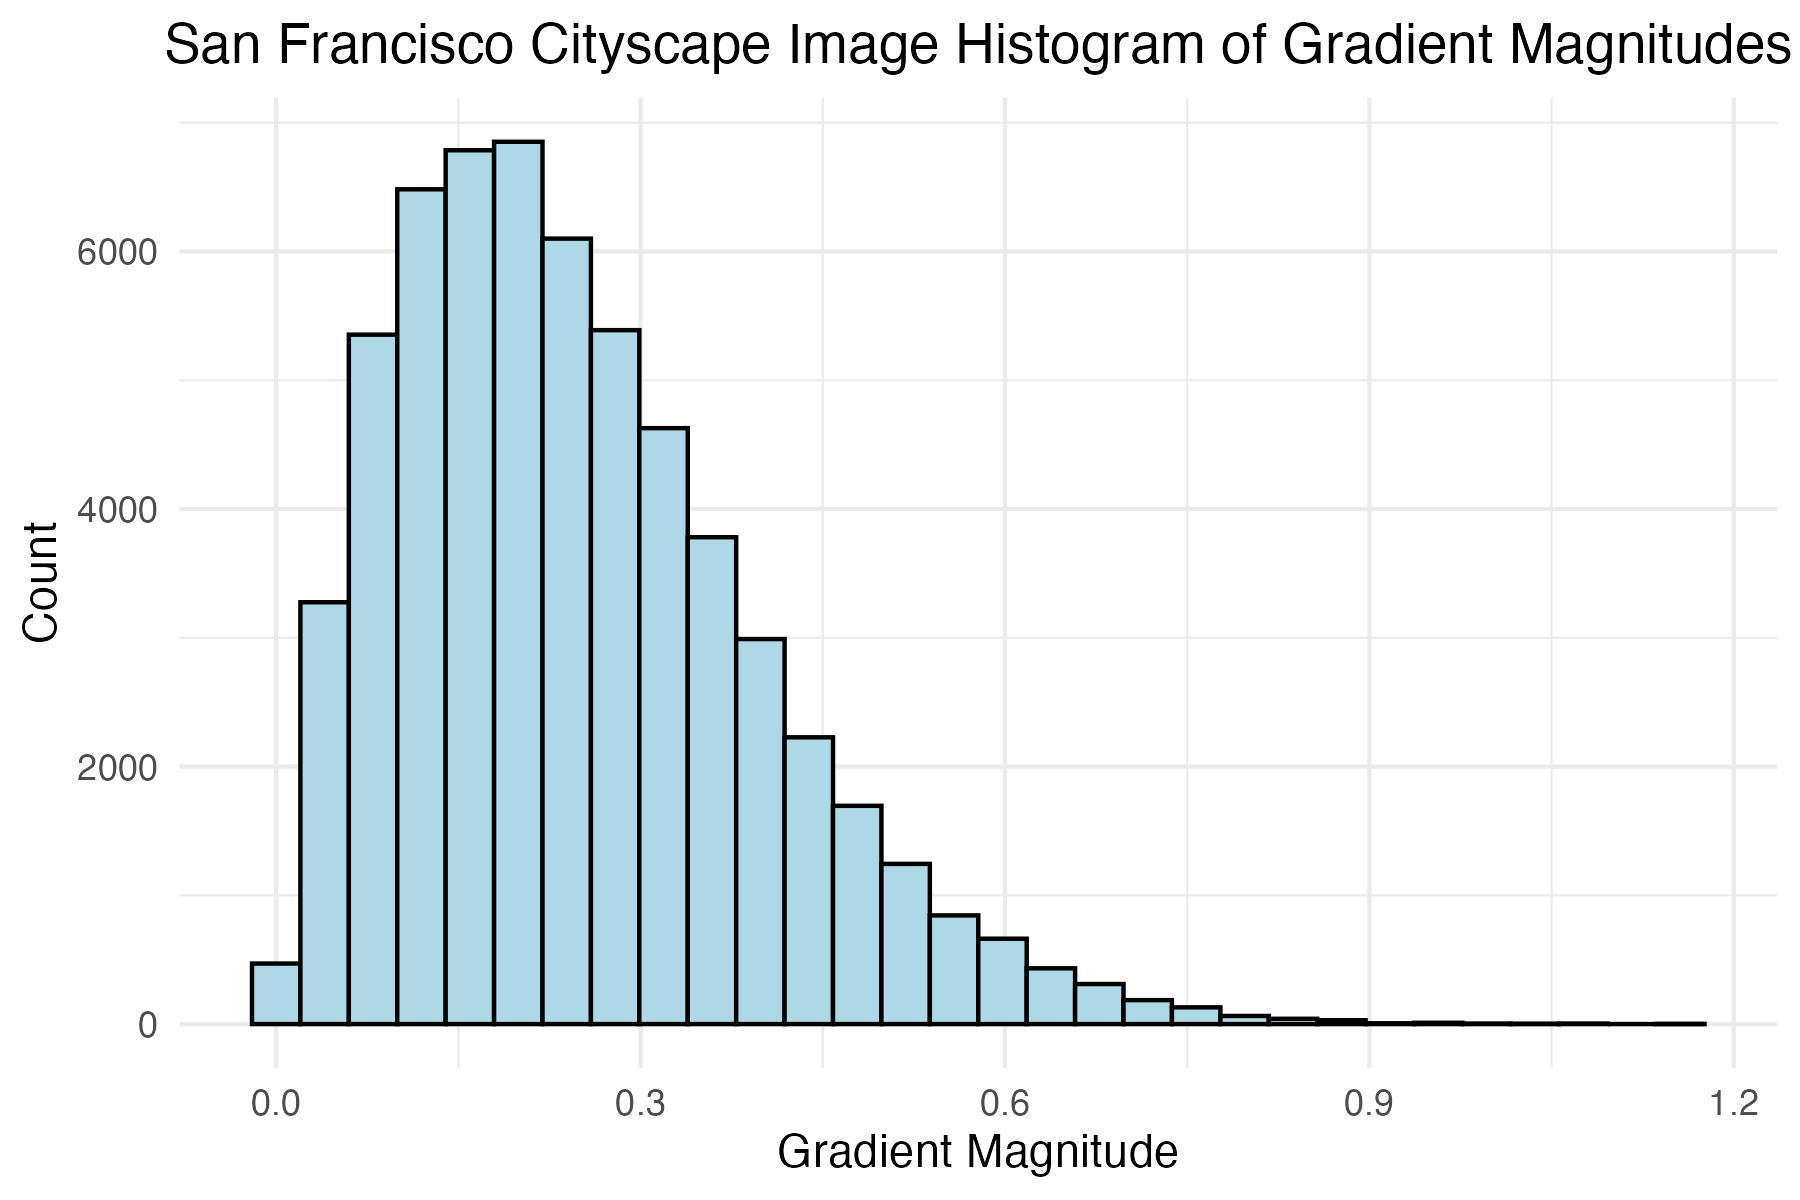
\includegraphics{images/plots/aerial_cities/sf_histogram_mag_plot.jpg}
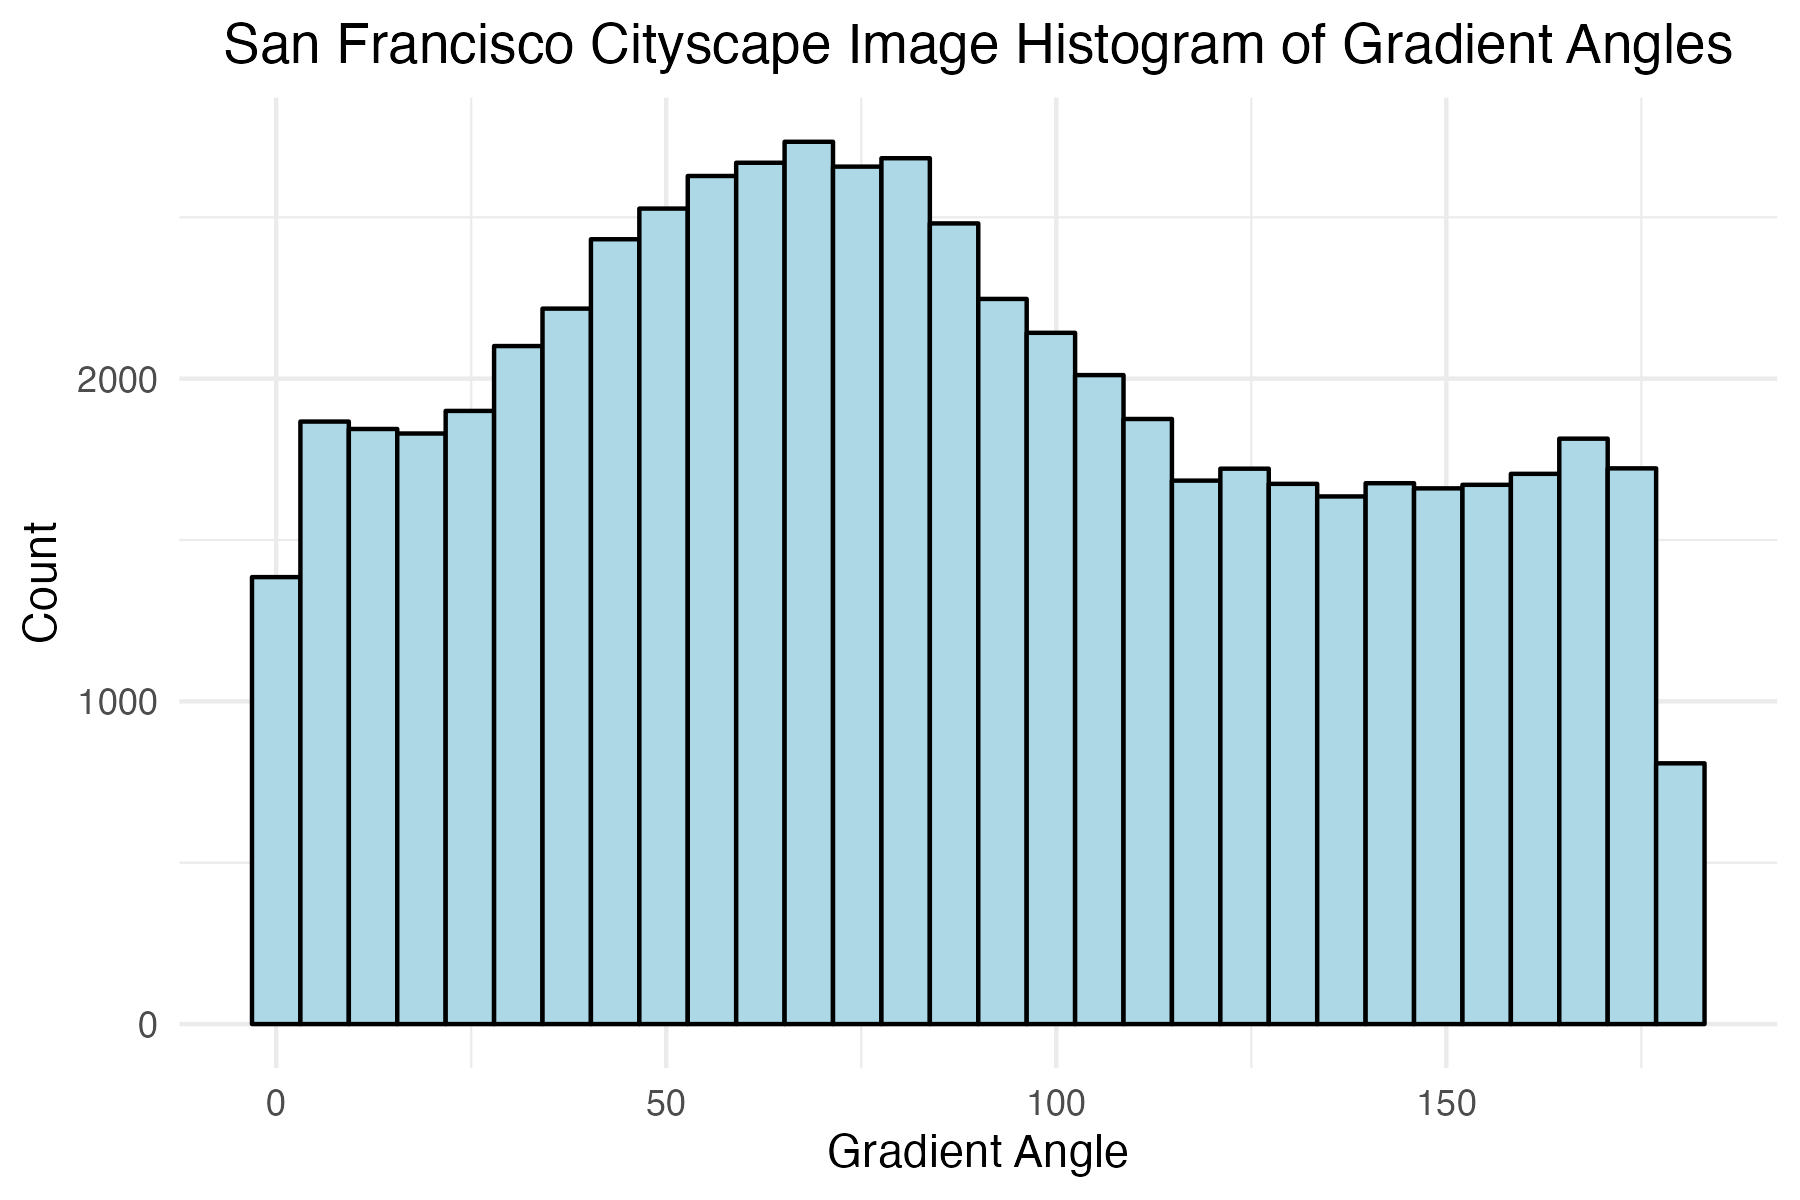
\includegraphics{images/plots/aerial_cities/sf_histogram_theta_plot.jpg}\end{minipage}%
%
\begin{minipage}{0.33\linewidth}
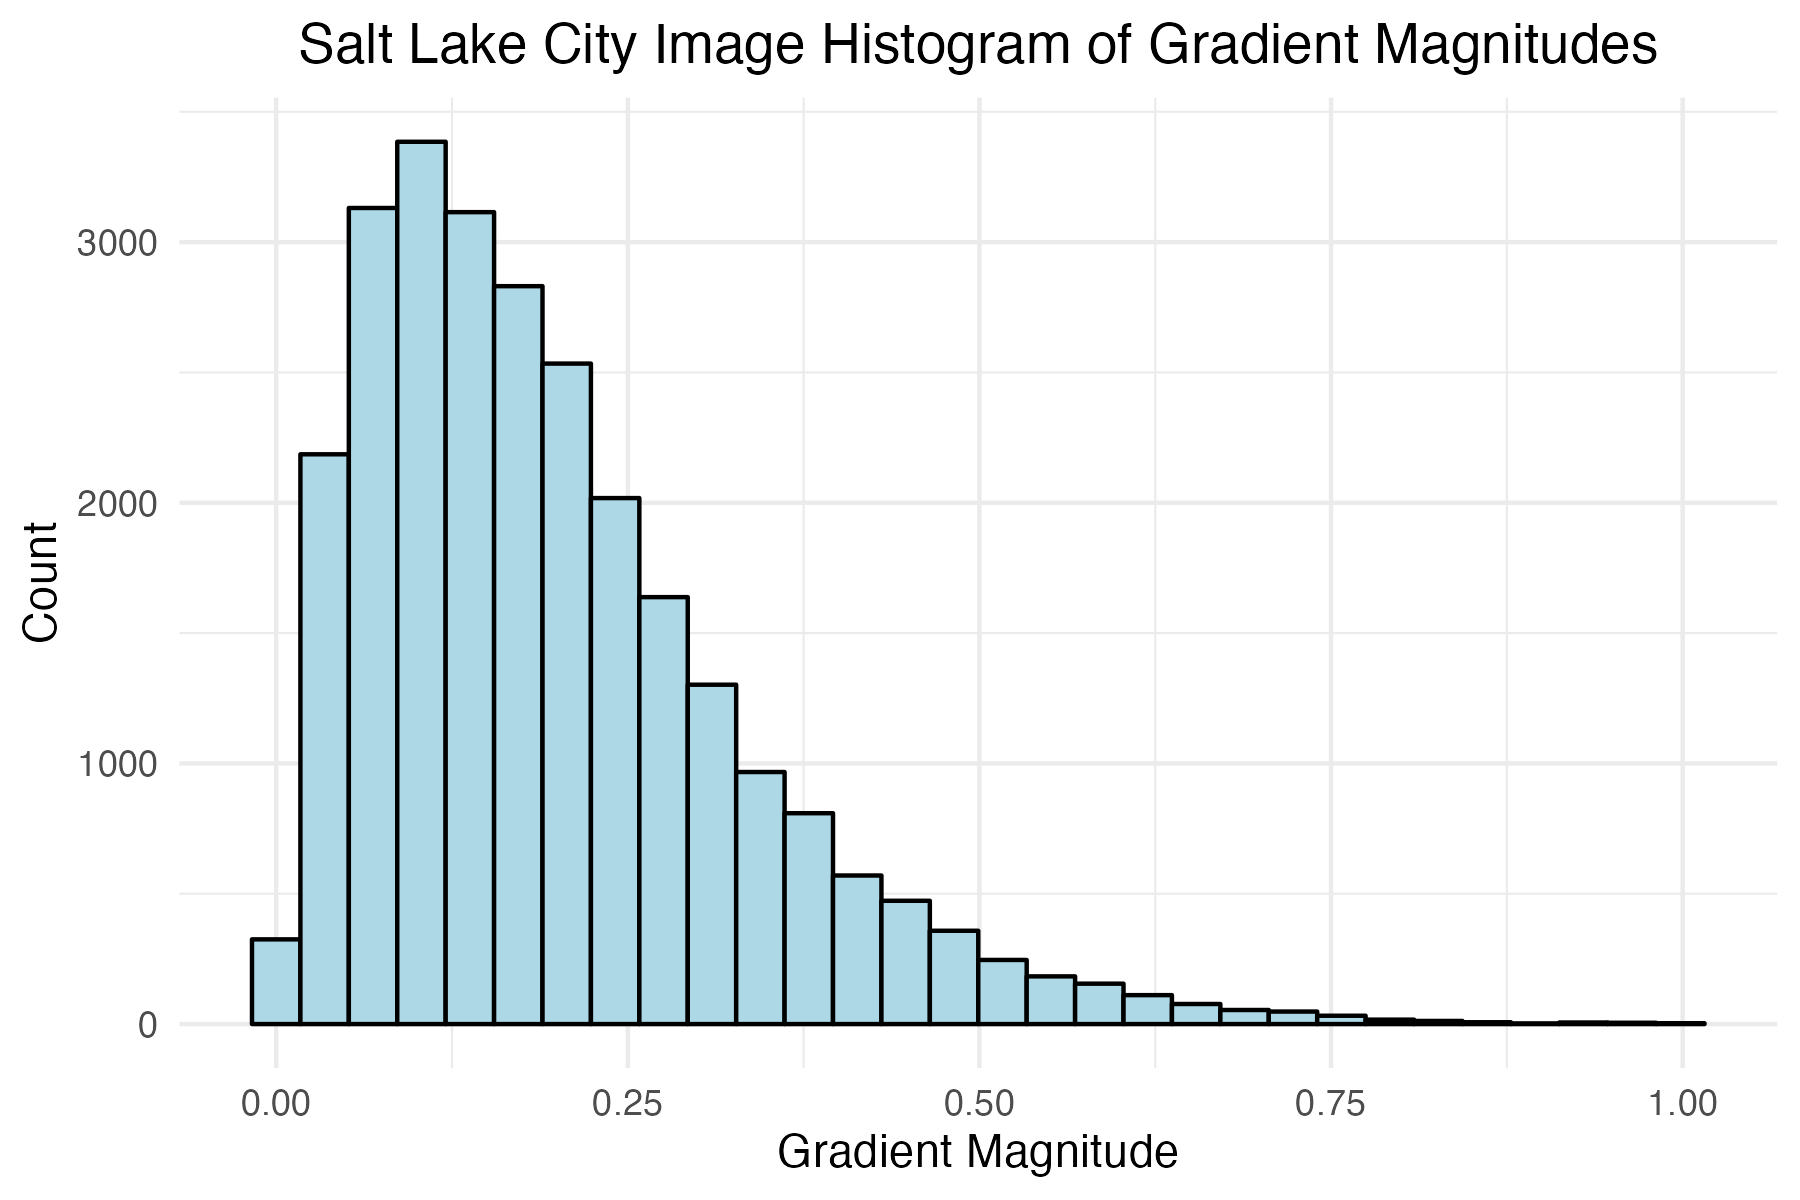
\includegraphics{images/plots/aerial_cities/salt_lake_histogram_mag_plot.jpg}
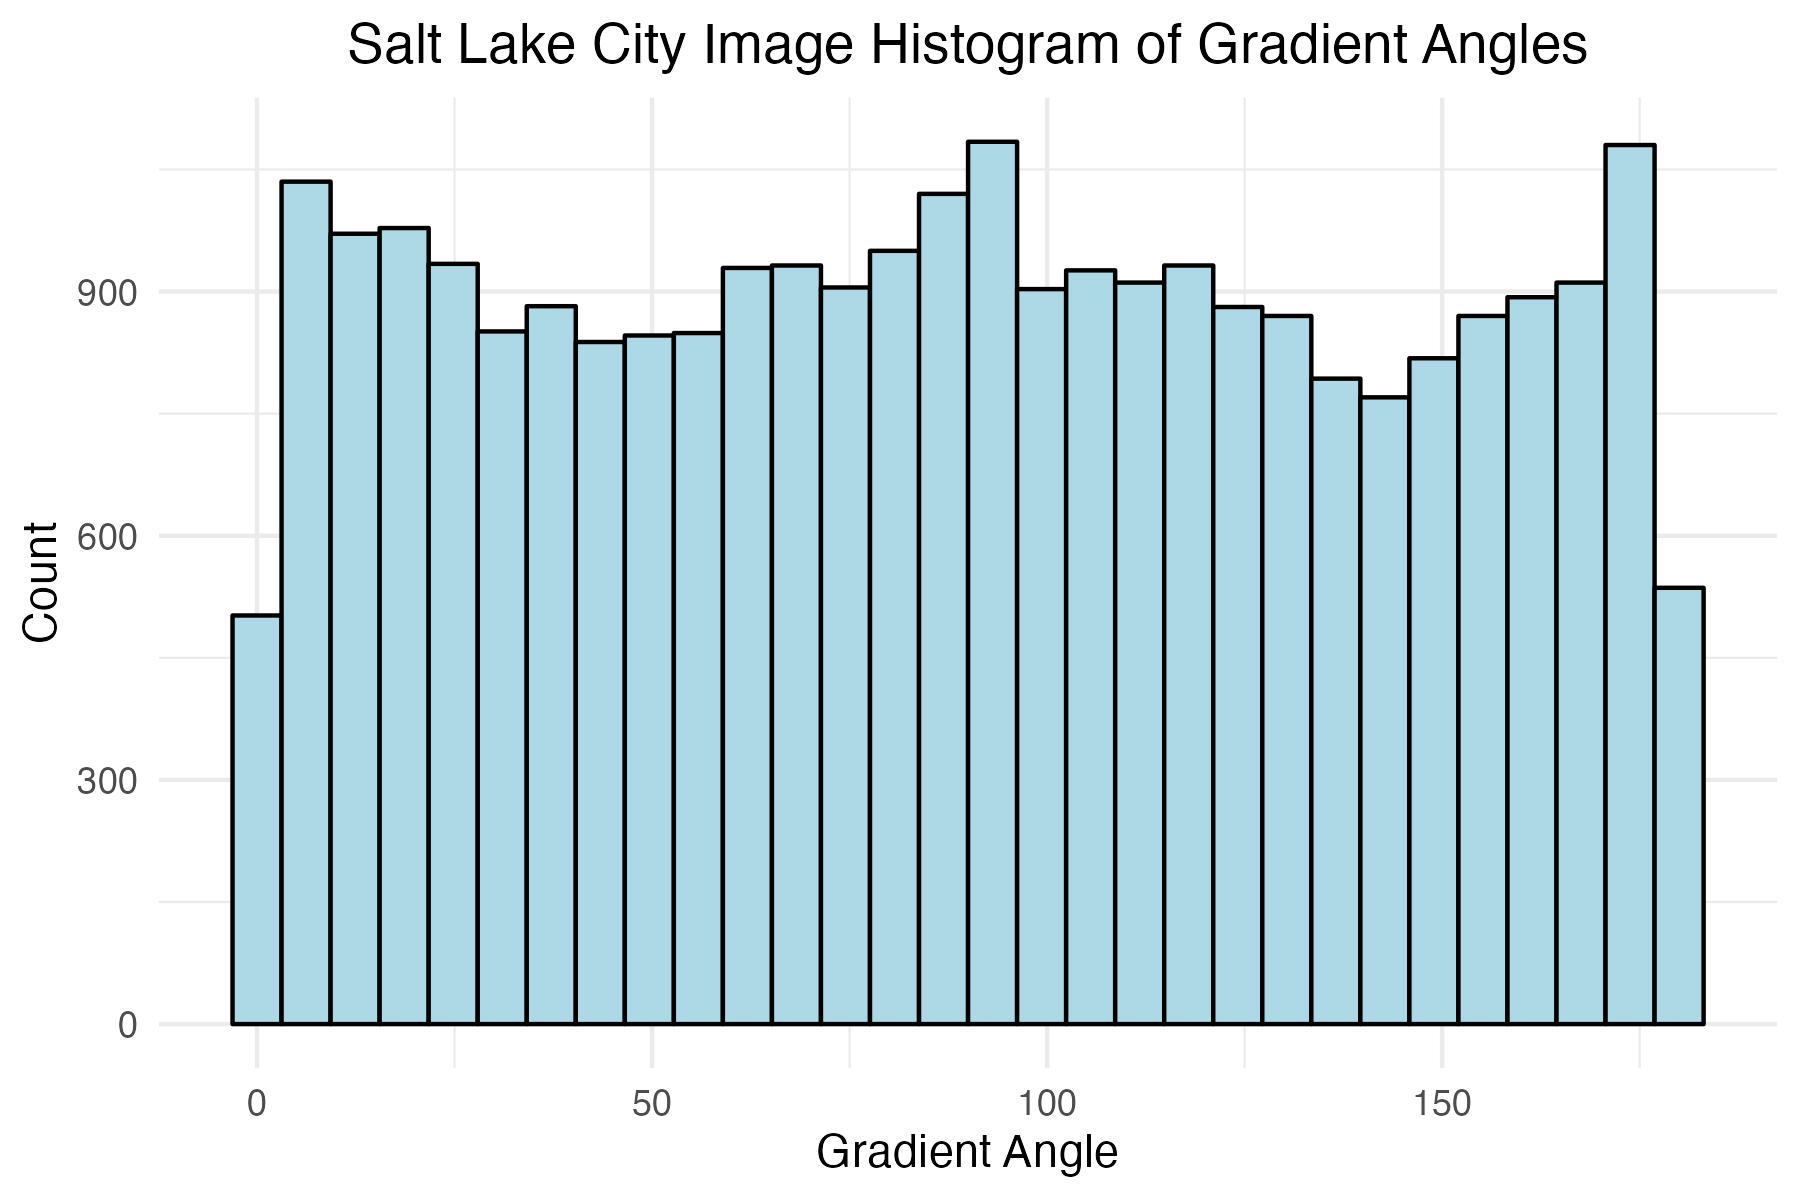
\includegraphics{images/plots/aerial_cities/salt_lake_histogram_theta_plot.jpg}\end{minipage}%
%
\begin{minipage}{0.33\linewidth}
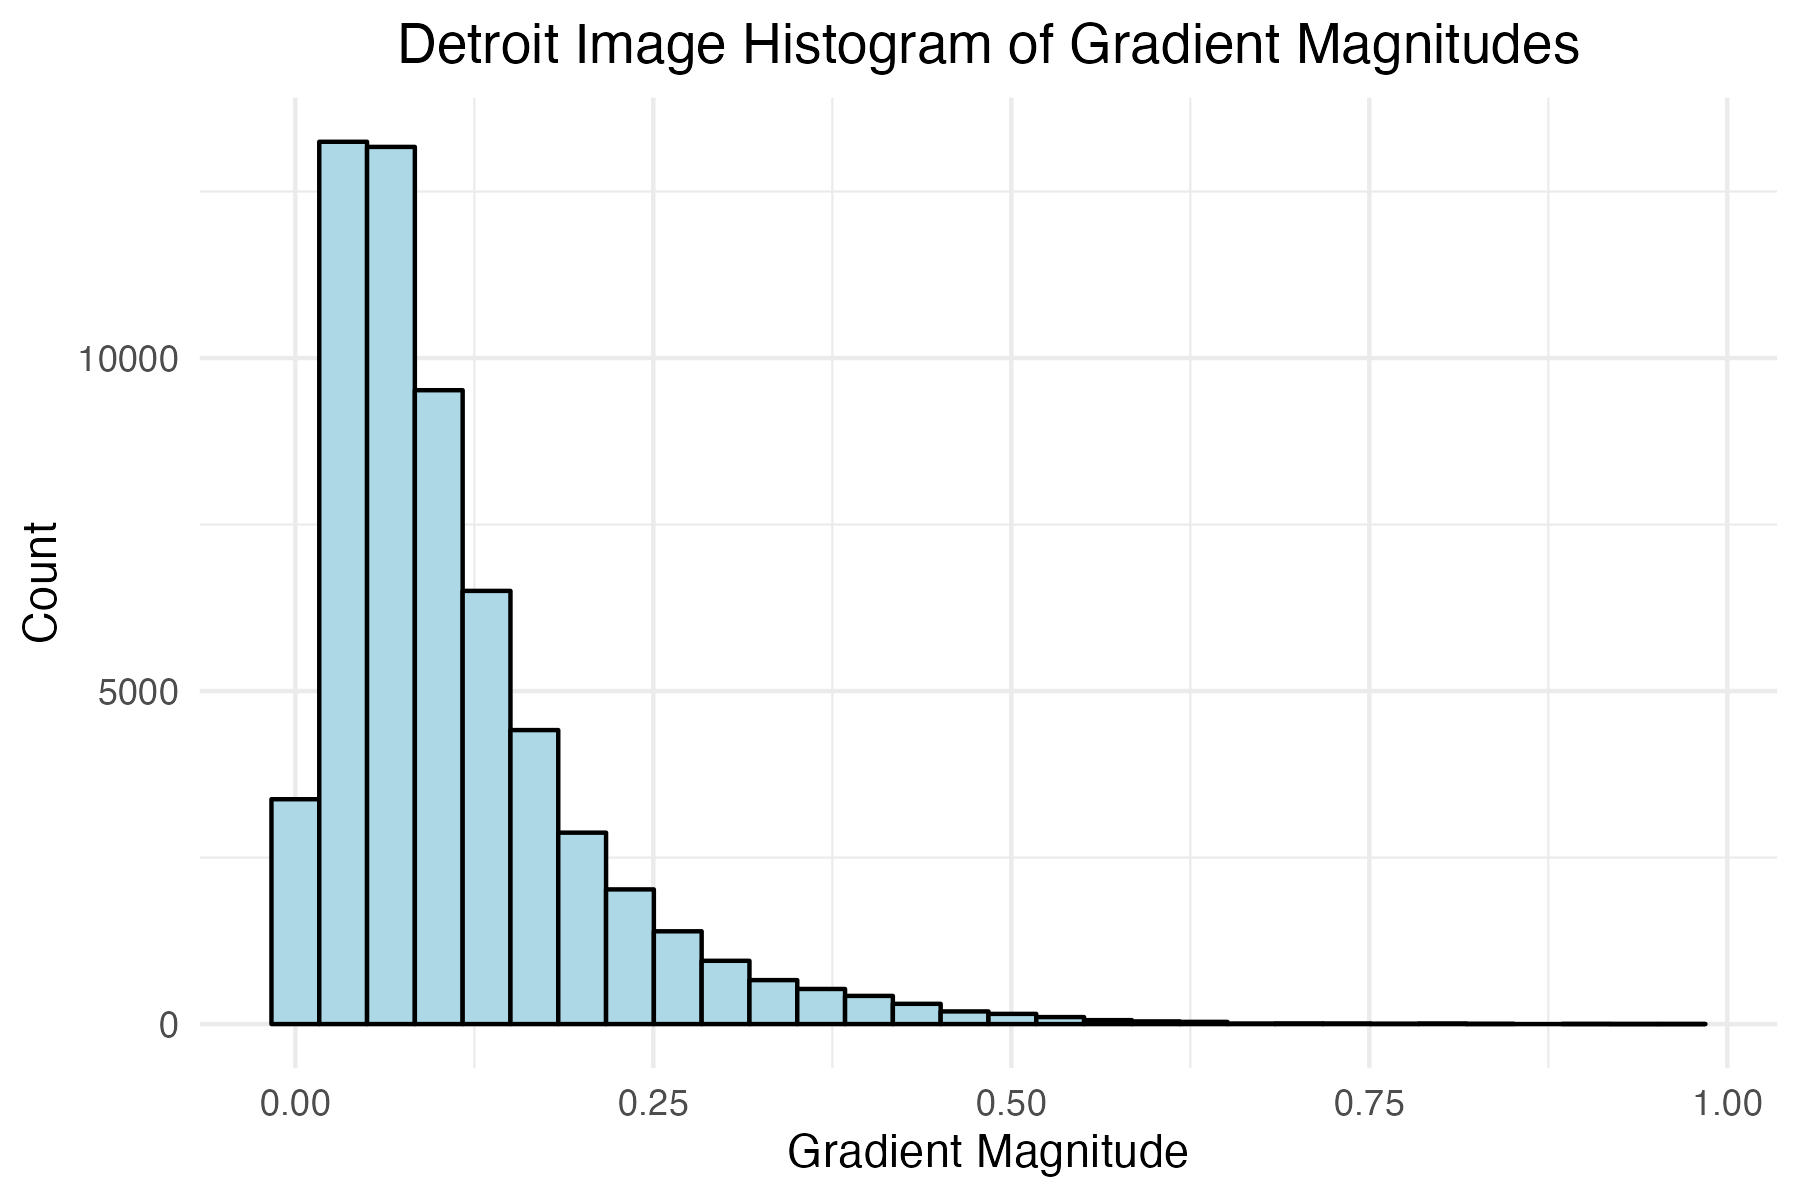
\includegraphics{images/plots/aerial_cities/detroit_histogram_mag_plot.jpg}
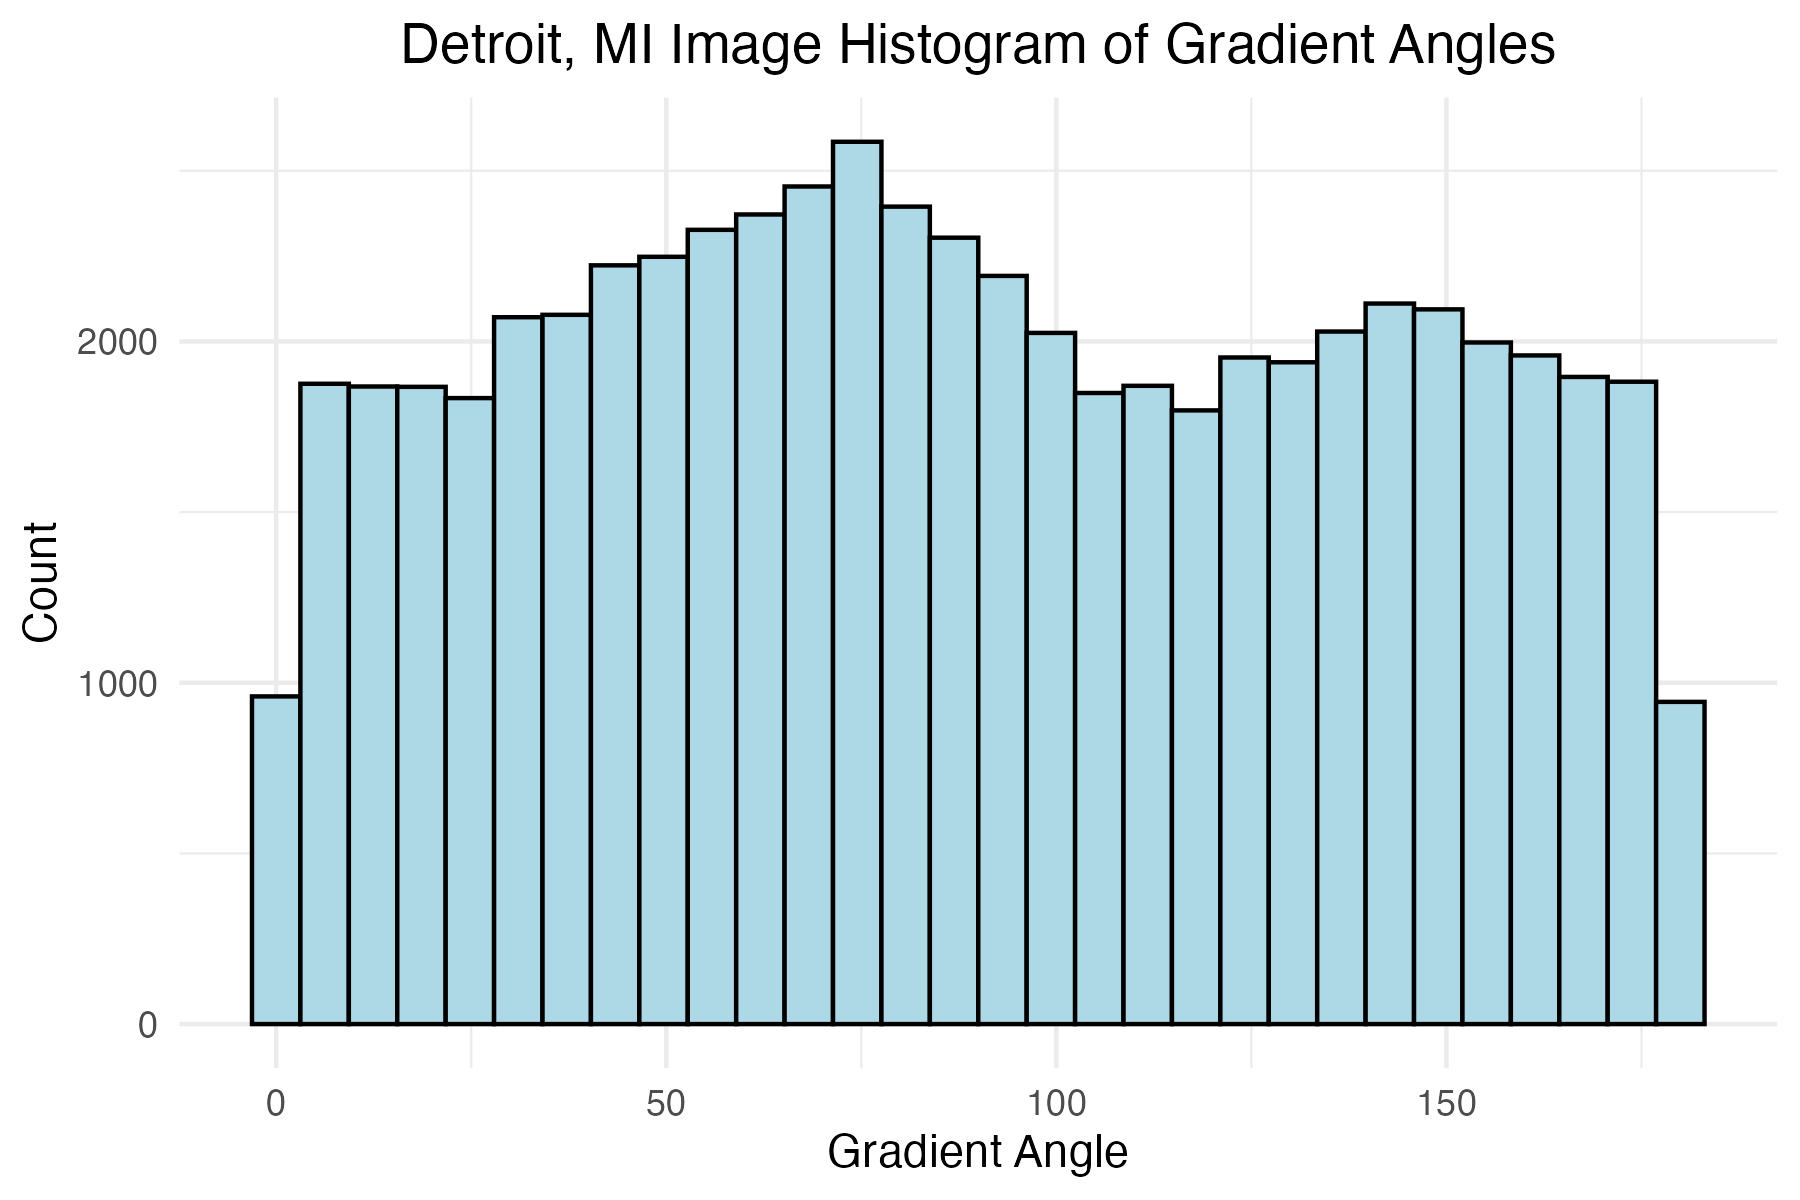
\includegraphics{images/plots/aerial_cities/detroit_histogram_theta_plot.jpg}\end{minipage}%

\caption{\label{fig-city-histograms}Aerial Cityscape Magnitudes and
Angles}

\end{figure}%

\section{Build New Distributed Histogram Data
Frames}\label{build-new-distributed-histogram-data-frames}

\begin{Shaded}
\begin{Highlighting}[]
\CommentTok{\# function to calculate the contributions to neighboring bins}
\NormalTok{calculate\_bin\_contributions }\OtherTok{\textless{}{-}} \ControlFlowTok{function}\NormalTok{(angle, magnitude, num\_bins) \{}
\NormalTok{  bin\_width }\OtherTok{\textless{}{-}} \DecValTok{180} \SpecialCharTok{/}\NormalTok{ num\_bins}
\NormalTok{  contributions }\OtherTok{\textless{}{-}} \FunctionTok{numeric}\NormalTok{(num\_bins)}
  
  \CommentTok{\# get the central bin}
\NormalTok{  central\_bin }\OtherTok{\textless{}{-}} \FunctionTok{floor}\NormalTok{(angle }\SpecialCharTok{/}\NormalTok{ bin\_width) }\SpecialCharTok{\%\%}\NormalTok{ num\_bins}
\NormalTok{  next\_bin }\OtherTok{\textless{}{-}}\NormalTok{ (central\_bin }\SpecialCharTok{+} \DecValTok{1}\NormalTok{) }\SpecialCharTok{\%\%}\NormalTok{ num\_bins}
  
  \CommentTok{\# get contributions to neighboring bins}
\NormalTok{  weight }\OtherTok{\textless{}{-}}\NormalTok{ (}\DecValTok{1} \SpecialCharTok{{-}} \FunctionTok{abs}\NormalTok{((angle }\SpecialCharTok{\%\%}\NormalTok{ bin\_width) }\SpecialCharTok{/}\NormalTok{ bin\_width)) }\SpecialCharTok{*}\NormalTok{ magnitude}
  
\NormalTok{  contributions[central\_bin }\SpecialCharTok{+} \DecValTok{1}\NormalTok{] }\OtherTok{\textless{}{-}}\NormalTok{ weight}
\NormalTok{  contributions[next\_bin }\SpecialCharTok{+} \DecValTok{1}\NormalTok{] }\OtherTok{\textless{}{-}}\NormalTok{ magnitude }\SpecialCharTok{{-}}\NormalTok{ weight}
  
  \FunctionTok{return}\NormalTok{(}\FunctionTok{list}\NormalTok{(contributions[}\DecValTok{1}\NormalTok{],}
\NormalTok{         contributions[}\DecValTok{2}\NormalTok{],}
\NormalTok{         contributions[}\DecValTok{3}\NormalTok{],}
\NormalTok{         contributions[}\DecValTok{4}\NormalTok{],}
\NormalTok{         contributions[}\DecValTok{5}\NormalTok{],}
\NormalTok{         contributions[}\DecValTok{6}\NormalTok{],}
\NormalTok{         contributions[}\DecValTok{7}\NormalTok{],}
\NormalTok{         contributions[}\DecValTok{8}\NormalTok{],}
\NormalTok{         contributions[}\DecValTok{9}\NormalTok{])}
\NormalTok{         )}
\NormalTok{\}}
\end{Highlighting}
\end{Shaded}

\begin{Shaded}
\begin{Highlighting}[]
\CommentTok{\# Create filtered data frames using the filter levels for magnitudes defined above, store all in a list}
\NormalTok{filtered\_aerial\_standard\_df\_list }\OtherTok{\textless{}{-}}\FunctionTok{list}\NormalTok{(sf\_hog\_df }\SpecialCharTok{\%\textgreater{}\%}
                                   \FunctionTok{filter}\NormalTok{(mag }\SpecialCharTok{\textgreater{}=}\NormalTok{ sf\_mag\_filter),}
\NormalTok{                                 salt\_lake\_hog\_df }\SpecialCharTok{\%\textgreater{}\%}
                                   \FunctionTok{filter}\NormalTok{(mag }\SpecialCharTok{\textgreater{}=}\NormalTok{ salt\_lake\_mag\_filter), }
\NormalTok{                                 detroit\_hog\_df }\SpecialCharTok{\%\textgreater{}\%}
                                   \FunctionTok{filter}\NormalTok{(mag }\SpecialCharTok{\textgreater{}=}\NormalTok{ detroit\_mag\_filter))}
\end{Highlighting}
\end{Shaded}

\begin{Shaded}
\begin{Highlighting}[]
\CommentTok{\# empty list for storing new distributed histogram data frames}
\NormalTok{aerial\_contribution\_df\_list }\OtherTok{\textless{}{-}} \FunctionTok{list}\NormalTok{()}

\CommentTok{\# Define the number of bins}
\NormalTok{num\_bins }\OtherTok{\textless{}{-}} \DecValTok{9}
 
\CommentTok{\# iterate through each filtered standard data frame}
\ControlFlowTok{for}\NormalTok{ (i }\ControlFlowTok{in} \DecValTok{1}\SpecialCharTok{:}\FunctionTok{length}\NormalTok{(filtered\_aerial\_standard\_df\_list))\{}
  
\NormalTok{  aerial\_contribution\_hog\_df }\OtherTok{\textless{}{-}} 
\NormalTok{    filtered\_aerial\_standard\_df\_list[[i]] }\SpecialCharTok{\%\textgreater{}\%}
    \FunctionTok{rowwise}\NormalTok{() }\SpecialCharTok{\%\textgreater{}\%}
    \FunctionTok{mutate}\NormalTok{(}\StringTok{\textasciigrave{}}\AttributeTok{0}\StringTok{\textasciigrave{}} \OtherTok{=} \FunctionTok{calculate\_bin\_contributions}\NormalTok{(theta, mag, }\DecValTok{9}\NormalTok{)[[}\DecValTok{1}\NormalTok{]],}
           \StringTok{\textasciigrave{}}\AttributeTok{20}\StringTok{\textasciigrave{}} \OtherTok{=} \FunctionTok{calculate\_bin\_contributions}\NormalTok{(theta, mag, }\DecValTok{9}\NormalTok{)[[}\DecValTok{2}\NormalTok{]],}
           \StringTok{\textasciigrave{}}\AttributeTok{40}\StringTok{\textasciigrave{}} \OtherTok{=} \FunctionTok{calculate\_bin\_contributions}\NormalTok{(theta, mag, }\DecValTok{9}\NormalTok{)[[}\DecValTok{3}\NormalTok{]],}
           \StringTok{\textasciigrave{}}\AttributeTok{60}\StringTok{\textasciigrave{}} \OtherTok{=} \FunctionTok{calculate\_bin\_contributions}\NormalTok{(theta, mag, }\DecValTok{9}\NormalTok{)[[}\DecValTok{4}\NormalTok{]],}
           \StringTok{\textasciigrave{}}\AttributeTok{80}\StringTok{\textasciigrave{}} \OtherTok{=} \FunctionTok{calculate\_bin\_contributions}\NormalTok{(theta, mag, }\DecValTok{9}\NormalTok{)[[}\DecValTok{5}\NormalTok{]],}
           \StringTok{\textasciigrave{}}\AttributeTok{100}\StringTok{\textasciigrave{}} \OtherTok{=} \FunctionTok{calculate\_bin\_contributions}\NormalTok{(theta, mag, }\DecValTok{9}\NormalTok{)[[}\DecValTok{6}\NormalTok{]],}
           \StringTok{\textasciigrave{}}\AttributeTok{120}\StringTok{\textasciigrave{}} \OtherTok{=} \FunctionTok{calculate\_bin\_contributions}\NormalTok{(theta, mag, }\DecValTok{9}\NormalTok{)[[}\DecValTok{7}\NormalTok{]],}
           \StringTok{\textasciigrave{}}\AttributeTok{140}\StringTok{\textasciigrave{}} \OtherTok{=} \FunctionTok{calculate\_bin\_contributions}\NormalTok{(theta, mag, }\DecValTok{9}\NormalTok{)[[}\DecValTok{8}\NormalTok{]],}
           \StringTok{\textasciigrave{}}\AttributeTok{160}\StringTok{\textasciigrave{}} \OtherTok{=} \FunctionTok{calculate\_bin\_contributions}\NormalTok{(theta, mag, }\DecValTok{9}\NormalTok{)[[}\DecValTok{9}\NormalTok{]],}
\NormalTok{           )}
  
  \CommentTok{\# rearrange into same tidy format}
\NormalTok{  aerial\_split\_histo\_df }\OtherTok{\textless{}{-}} 
\NormalTok{    aerial\_contribution\_hog\_df }\SpecialCharTok{\%\textgreater{}\%}
    \FunctionTok{pivot\_longer}\NormalTok{(}\AttributeTok{names\_to =} \StringTok{"bin"}\NormalTok{, }
                 \AttributeTok{values\_to =} \StringTok{"contribution"}\NormalTok{, }
                 \AttributeTok{cols =} \DecValTok{4}\SpecialCharTok{:}\FunctionTok{ncol}\NormalTok{(aerial\_contribution\_hog\_df)) }\SpecialCharTok{\%\textgreater{}\%}
    \FunctionTok{mutate}\NormalTok{(}\AttributeTok{bin =} \FunctionTok{as.numeric}\NormalTok{(bin)) }\SpecialCharTok{\%\textgreater{}\%}
    \FunctionTok{group\_by}\NormalTok{(bin) }\SpecialCharTok{\%\textgreater{}\%}
    \FunctionTok{summarise}\NormalTok{(}\AttributeTok{contribution\_sum =} \FunctionTok{sum}\NormalTok{(contribution))}
  
  \CommentTok{\# add to list for storage}
\NormalTok{  aerial\_contribution\_df\_list[[i]] }\OtherTok{\textless{}{-}}\NormalTok{ aerial\_split\_histo\_df}

\NormalTok{\}}
\end{Highlighting}
\end{Shaded}

\section{Generate Polar Plots for Images Using Standard Histogram
Binning
Technique}\label{generate-polar-plots-for-images-using-standard-histogram-binning-technique}

\begin{Shaded}
\begin{Highlighting}[]
\CommentTok{\# SF polar plot}
\NormalTok{sf\_plot }\OtherTok{\textless{}{-}}
  \FunctionTok{ggplot}\NormalTok{(filtered\_aerial\_standard\_df\_list[[}\DecValTok{1}\NormalTok{]], }
         \FunctionTok{aes}\NormalTok{(}\AttributeTok{x =}\NormalTok{ theta)) }\SpecialCharTok{+}
  \FunctionTok{geom\_histogram}\NormalTok{(}\AttributeTok{colour =} \StringTok{"black"}\NormalTok{, }
                 \AttributeTok{fill =} \StringTok{"lightblue"}\NormalTok{, }
                 \AttributeTok{breaks =} \FunctionTok{seq}\NormalTok{(}\DecValTok{0}\NormalTok{, }\DecValTok{360}\NormalTok{, }\AttributeTok{length.out =} \FloatTok{17.5}\NormalTok{),}
                 \AttributeTok{bins =} \DecValTok{9}\NormalTok{) }\SpecialCharTok{+}
  \FunctionTok{coord\_polar}\NormalTok{(}
    \AttributeTok{theta =} \StringTok{"x"}\NormalTok{, }
    \AttributeTok{start =} \DecValTok{0}\NormalTok{, }
    \AttributeTok{direction =} \DecValTok{1}\NormalTok{) }\SpecialCharTok{+}
  \FunctionTok{scale\_x\_continuous}\NormalTok{(}\AttributeTok{limits =} \FunctionTok{c}\NormalTok{(}\DecValTok{0}\NormalTok{,}\DecValTok{360}\NormalTok{),}
    \AttributeTok{breaks =} \FunctionTok{c}\NormalTok{(}\DecValTok{0}\NormalTok{, }\DecValTok{45}\NormalTok{, }\DecValTok{90}\NormalTok{, }\DecValTok{135}\NormalTok{, }\DecValTok{180}\NormalTok{, }\DecValTok{225}\NormalTok{, }\DecValTok{270}\NormalTok{, }\DecValTok{315}\NormalTok{), }
    \AttributeTok{labels =} \FunctionTok{c}\NormalTok{(}\StringTok{"N"}\NormalTok{, }\StringTok{"NE"}\NormalTok{, }\StringTok{"E"}\NormalTok{, }\StringTok{"SE"}\NormalTok{, }\StringTok{"S"}\NormalTok{, }\StringTok{"SW"}\NormalTok{, }\StringTok{"W"}\NormalTok{, }\StringTok{"NW"}\NormalTok{)}
\NormalTok{  )}\SpecialCharTok{+}
  \FunctionTok{labs}\NormalTok{(}\AttributeTok{title =} \StringTok{"Polar Plot of San Francisco, CA Image}\SpecialCharTok{\textbackslash{}n}\StringTok{Using Standard HOG Technique"}\NormalTok{) }\SpecialCharTok{+}
  \FunctionTok{theme\_minimal}\NormalTok{() }\SpecialCharTok{+}
  \FunctionTok{labs}\NormalTok{(}\AttributeTok{x =} \StringTok{""}\NormalTok{) }\SpecialCharTok{+}
  \FunctionTok{theme}\NormalTok{(}\AttributeTok{axis.title.y =} \FunctionTok{element\_blank}\NormalTok{(),}
        \AttributeTok{plot.title =} \FunctionTok{element\_text}\NormalTok{(}\AttributeTok{hjust =} \FloatTok{0.5}\NormalTok{))}

\CommentTok{\# save image}
\FunctionTok{ggsave}\NormalTok{(}\StringTok{"images/plots/aerial\_cities/sf\_standard\_polar\_plot.jpg"}\NormalTok{, sf\_plot, }\AttributeTok{width =} \DecValTok{6}\NormalTok{, }\AttributeTok{height =} \DecValTok{4}\NormalTok{, }\AttributeTok{dpi =} \DecValTok{300}\NormalTok{)}
\end{Highlighting}
\end{Shaded}

\begin{Shaded}
\begin{Highlighting}[]
\CommentTok{\# SLC plot}
\NormalTok{salt\_lake\_plot }\OtherTok{\textless{}{-}}
  \FunctionTok{ggplot}\NormalTok{(filtered\_aerial\_standard\_df\_list[[}\DecValTok{2}\NormalTok{]], }
         \FunctionTok{aes}\NormalTok{(}\AttributeTok{x =}\NormalTok{ theta)) }\SpecialCharTok{+}
  \FunctionTok{geom\_histogram}\NormalTok{(}\AttributeTok{colour =} \StringTok{"black"}\NormalTok{, }
                 \AttributeTok{fill =} \StringTok{"lightblue"}\NormalTok{, }
                 \AttributeTok{breaks =} \FunctionTok{seq}\NormalTok{(}\DecValTok{0}\NormalTok{, }\DecValTok{360}\NormalTok{, }\AttributeTok{length.out =} \FloatTok{17.5}\NormalTok{),}
                 \AttributeTok{bins =} \DecValTok{9}\NormalTok{) }\SpecialCharTok{+}
  \FunctionTok{coord\_polar}\NormalTok{(}
    \AttributeTok{theta =} \StringTok{"x"}\NormalTok{, }
    \AttributeTok{start =} \DecValTok{0}\NormalTok{, }
    \AttributeTok{direction =} \DecValTok{1}\NormalTok{) }\SpecialCharTok{+}
  \FunctionTok{scale\_x\_continuous}\NormalTok{(}\AttributeTok{limits =} \FunctionTok{c}\NormalTok{(}\DecValTok{0}\NormalTok{,}\DecValTok{360}\NormalTok{),}
    \AttributeTok{breaks =} \FunctionTok{c}\NormalTok{(}\DecValTok{0}\NormalTok{, }\DecValTok{45}\NormalTok{, }\DecValTok{90}\NormalTok{, }\DecValTok{135}\NormalTok{, }\DecValTok{180}\NormalTok{, }\DecValTok{225}\NormalTok{, }\DecValTok{270}\NormalTok{, }\DecValTok{315}\NormalTok{), }
    \AttributeTok{labels =} \FunctionTok{c}\NormalTok{(}\StringTok{"N"}\NormalTok{, }\StringTok{"NE"}\NormalTok{, }\StringTok{"E"}\NormalTok{, }\StringTok{"SE"}\NormalTok{, }\StringTok{"S"}\NormalTok{, }\StringTok{"SW"}\NormalTok{, }\StringTok{"W"}\NormalTok{, }\StringTok{"NW"}\NormalTok{)}
\NormalTok{  )}\SpecialCharTok{+}
  \FunctionTok{labs}\NormalTok{(}\AttributeTok{title =} \StringTok{"Polar Plot of Salt Lake City, UT Image}\SpecialCharTok{\textbackslash{}n}\StringTok{Using Standard HOG Technique"}\NormalTok{) }\SpecialCharTok{+}
  \FunctionTok{theme\_minimal}\NormalTok{() }\SpecialCharTok{+}
  \FunctionTok{labs}\NormalTok{(}\AttributeTok{x =} \StringTok{""}\NormalTok{) }\SpecialCharTok{+}
  \FunctionTok{theme}\NormalTok{(}\AttributeTok{axis.title.y =} \FunctionTok{element\_blank}\NormalTok{(),}
        \AttributeTok{plot.title =} \FunctionTok{element\_text}\NormalTok{(}\AttributeTok{hjust =} \FloatTok{0.5}\NormalTok{))}

\CommentTok{\# save image}
\FunctionTok{ggsave}\NormalTok{(}\StringTok{"images/plots/aerial\_cities/salt\_lake\_standard\_polar\_plot.jpg"}\NormalTok{, salt\_lake\_plot, }\AttributeTok{width =} \DecValTok{6}\NormalTok{, }\AttributeTok{height =} \DecValTok{4}\NormalTok{, }\AttributeTok{dpi =} \DecValTok{300}\NormalTok{)}
\end{Highlighting}
\end{Shaded}

\begin{Shaded}
\begin{Highlighting}[]
\CommentTok{\# Detroit plot}
\NormalTok{detroit\_plot }\OtherTok{\textless{}{-}}
  \FunctionTok{ggplot}\NormalTok{(filtered\_aerial\_standard\_df\_list[[}\DecValTok{3}\NormalTok{]], }
         \FunctionTok{aes}\NormalTok{(}\AttributeTok{x =}\NormalTok{ theta)) }\SpecialCharTok{+}
  \FunctionTok{geom\_histogram}\NormalTok{(}\AttributeTok{colour =} \StringTok{"black"}\NormalTok{, }
                 \AttributeTok{fill =} \StringTok{"lightblue"}\NormalTok{, }
                 \AttributeTok{breaks =} \FunctionTok{seq}\NormalTok{(}\DecValTok{0}\NormalTok{, }\DecValTok{360}\NormalTok{, }\AttributeTok{length.out =} \FloatTok{17.5}\NormalTok{),}
                 \AttributeTok{bins =} \DecValTok{9}\NormalTok{) }\SpecialCharTok{+}
  \FunctionTok{coord\_polar}\NormalTok{(}
    \AttributeTok{theta =} \StringTok{"x"}\NormalTok{, }
    \AttributeTok{start =} \DecValTok{0}\NormalTok{, }
    \AttributeTok{direction =} \DecValTok{1}\NormalTok{) }\SpecialCharTok{+}
  \FunctionTok{scale\_x\_continuous}\NormalTok{(}\AttributeTok{limits =} \FunctionTok{c}\NormalTok{(}\DecValTok{0}\NormalTok{,}\DecValTok{360}\NormalTok{),}
    \AttributeTok{breaks =} \FunctionTok{c}\NormalTok{(}\DecValTok{0}\NormalTok{, }\DecValTok{45}\NormalTok{, }\DecValTok{90}\NormalTok{, }\DecValTok{135}\NormalTok{, }\DecValTok{180}\NormalTok{, }\DecValTok{225}\NormalTok{, }\DecValTok{270}\NormalTok{, }\DecValTok{315}\NormalTok{), }
    \AttributeTok{labels =} \FunctionTok{c}\NormalTok{(}\StringTok{"N"}\NormalTok{, }\StringTok{"NE"}\NormalTok{, }\StringTok{"E"}\NormalTok{, }\StringTok{"SE"}\NormalTok{, }\StringTok{"S"}\NormalTok{, }\StringTok{"SW"}\NormalTok{, }\StringTok{"W"}\NormalTok{, }\StringTok{"NW"}\NormalTok{)}
\NormalTok{  )}\SpecialCharTok{+}
  \FunctionTok{labs}\NormalTok{(}\AttributeTok{title =} \StringTok{"Polar Plot of Detroit, MI Image}\SpecialCharTok{\textbackslash{}n}\StringTok{Using Standard HOG Technique"}\NormalTok{) }\SpecialCharTok{+}
  \FunctionTok{theme\_minimal}\NormalTok{() }\SpecialCharTok{+}
  \FunctionTok{labs}\NormalTok{(}\AttributeTok{x =} \StringTok{""}\NormalTok{) }\SpecialCharTok{+}
  \FunctionTok{theme}\NormalTok{(}\AttributeTok{axis.title.y =} \FunctionTok{element\_blank}\NormalTok{(),}
        \AttributeTok{plot.title =} \FunctionTok{element\_text}\NormalTok{(}\AttributeTok{hjust =} \FloatTok{0.5}\NormalTok{))}

\CommentTok{\# save image}
\FunctionTok{ggsave}\NormalTok{(}\StringTok{"images/plots/aerial\_cities/detroit\_standard\_polar\_plot.jpg"}\NormalTok{, detroit\_plot, }\AttributeTok{width =} \DecValTok{6}\NormalTok{, }\AttributeTok{height =} \DecValTok{4}\NormalTok{, }\AttributeTok{dpi =} \DecValTok{300}\NormalTok{)}
\end{Highlighting}
\end{Shaded}

\begin{Shaded}
\begin{Highlighting}[]
\CommentTok{\# Save to an arranged image}
\NormalTok{all\_standard\_city\_plots }\OtherTok{\textless{}{-}}\NormalTok{ ggpubr}\SpecialCharTok{::}\FunctionTok{ggarrange}\NormalTok{(sf\_plot, }
\NormalTok{                                             salt\_lake\_plot, }
\NormalTok{                                             detroit\_plot)}

\FunctionTok{ggsave}\NormalTok{(}\StringTok{"images/plots/aerial\_cities/all\_standard\_polar\_plots.jpg"}\NormalTok{, }
\NormalTok{       all\_standard\_city\_plots, }
       \AttributeTok{width =} \DecValTok{7}\NormalTok{, }
       \AttributeTok{height =} \DecValTok{7}\NormalTok{)}
\end{Highlighting}
\end{Shaded}

\begin{figure}

\begin{minipage}{0.33\linewidth}

\begin{figure}[H]

{\centering 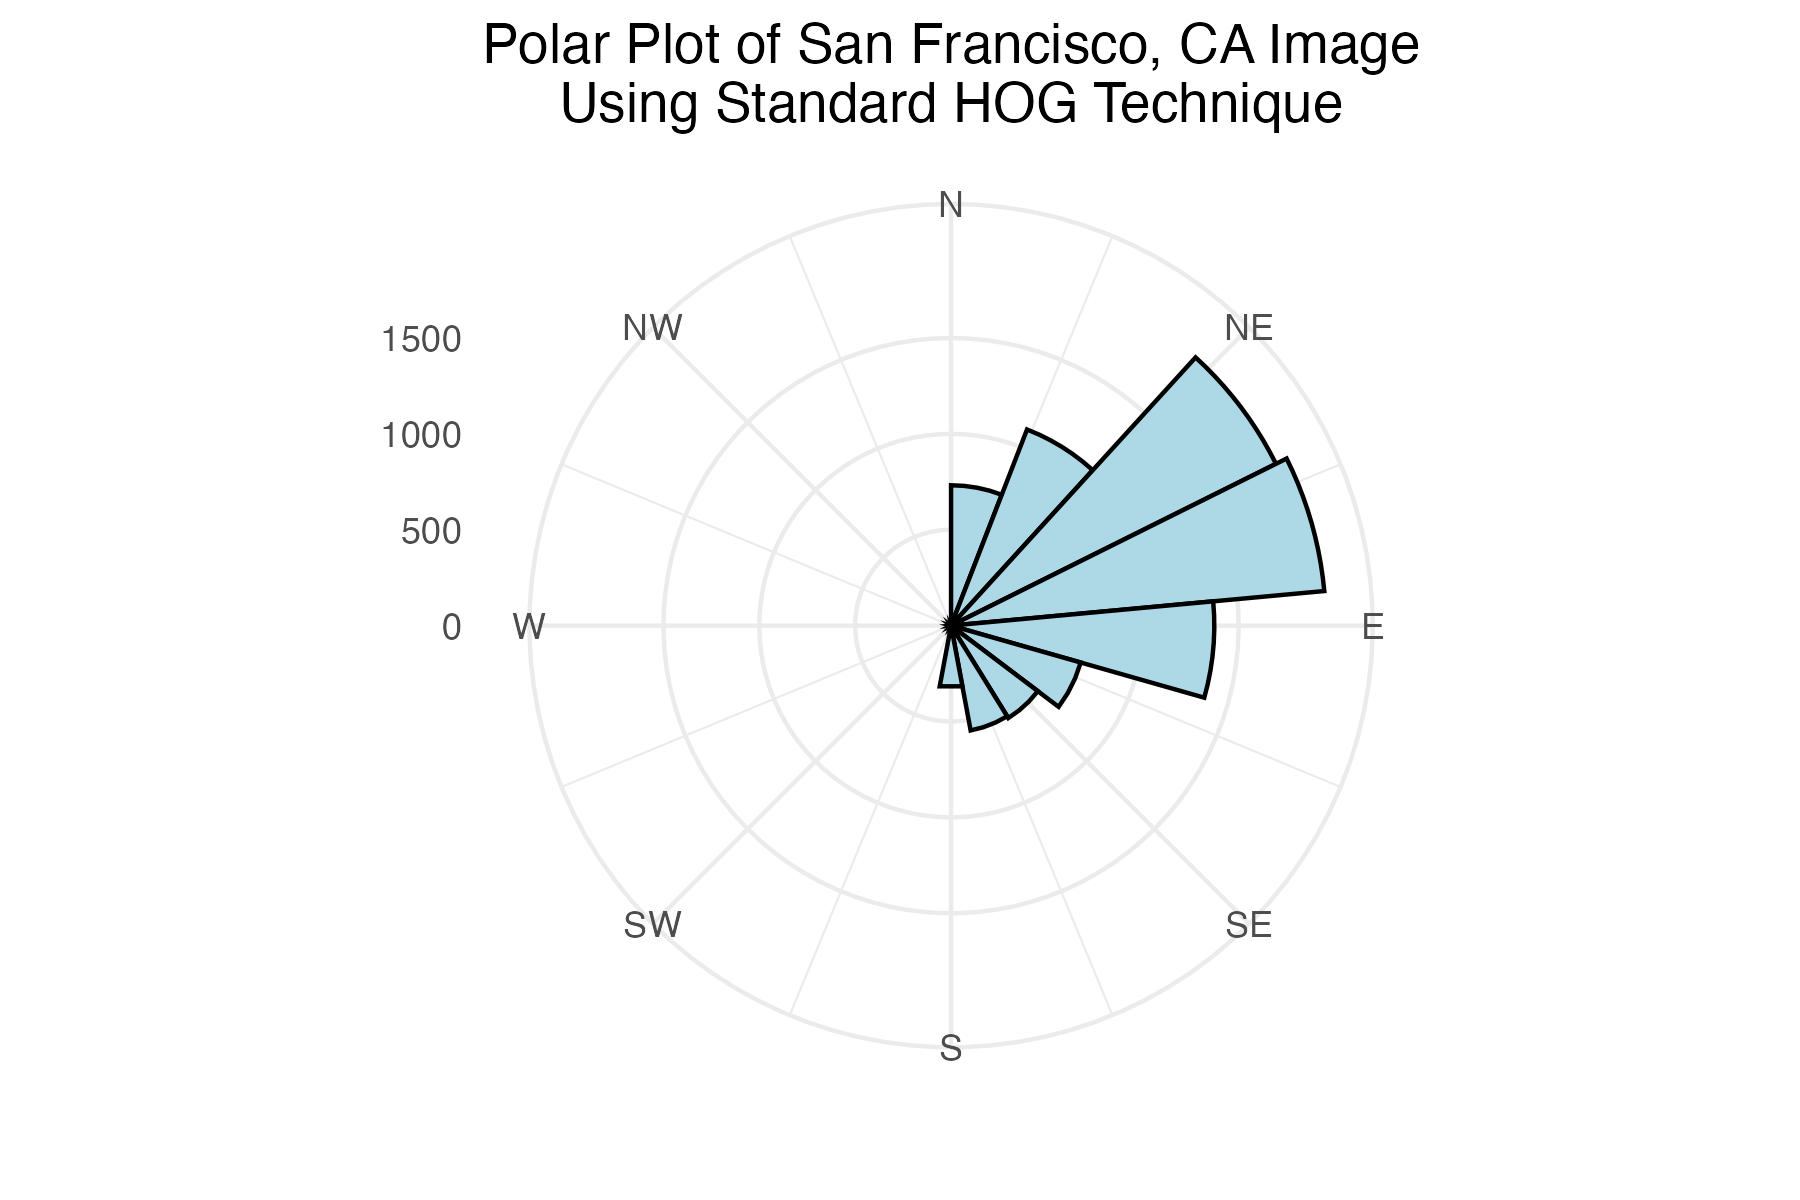
\includegraphics{images/plots/aerial_cities/sf_standard_polar_plot.jpg}

}

\subcaption{San Francisco, CA}

\end{figure}%

\end{minipage}%
%
\begin{minipage}{0.33\linewidth}

\begin{figure}[H]

{\centering 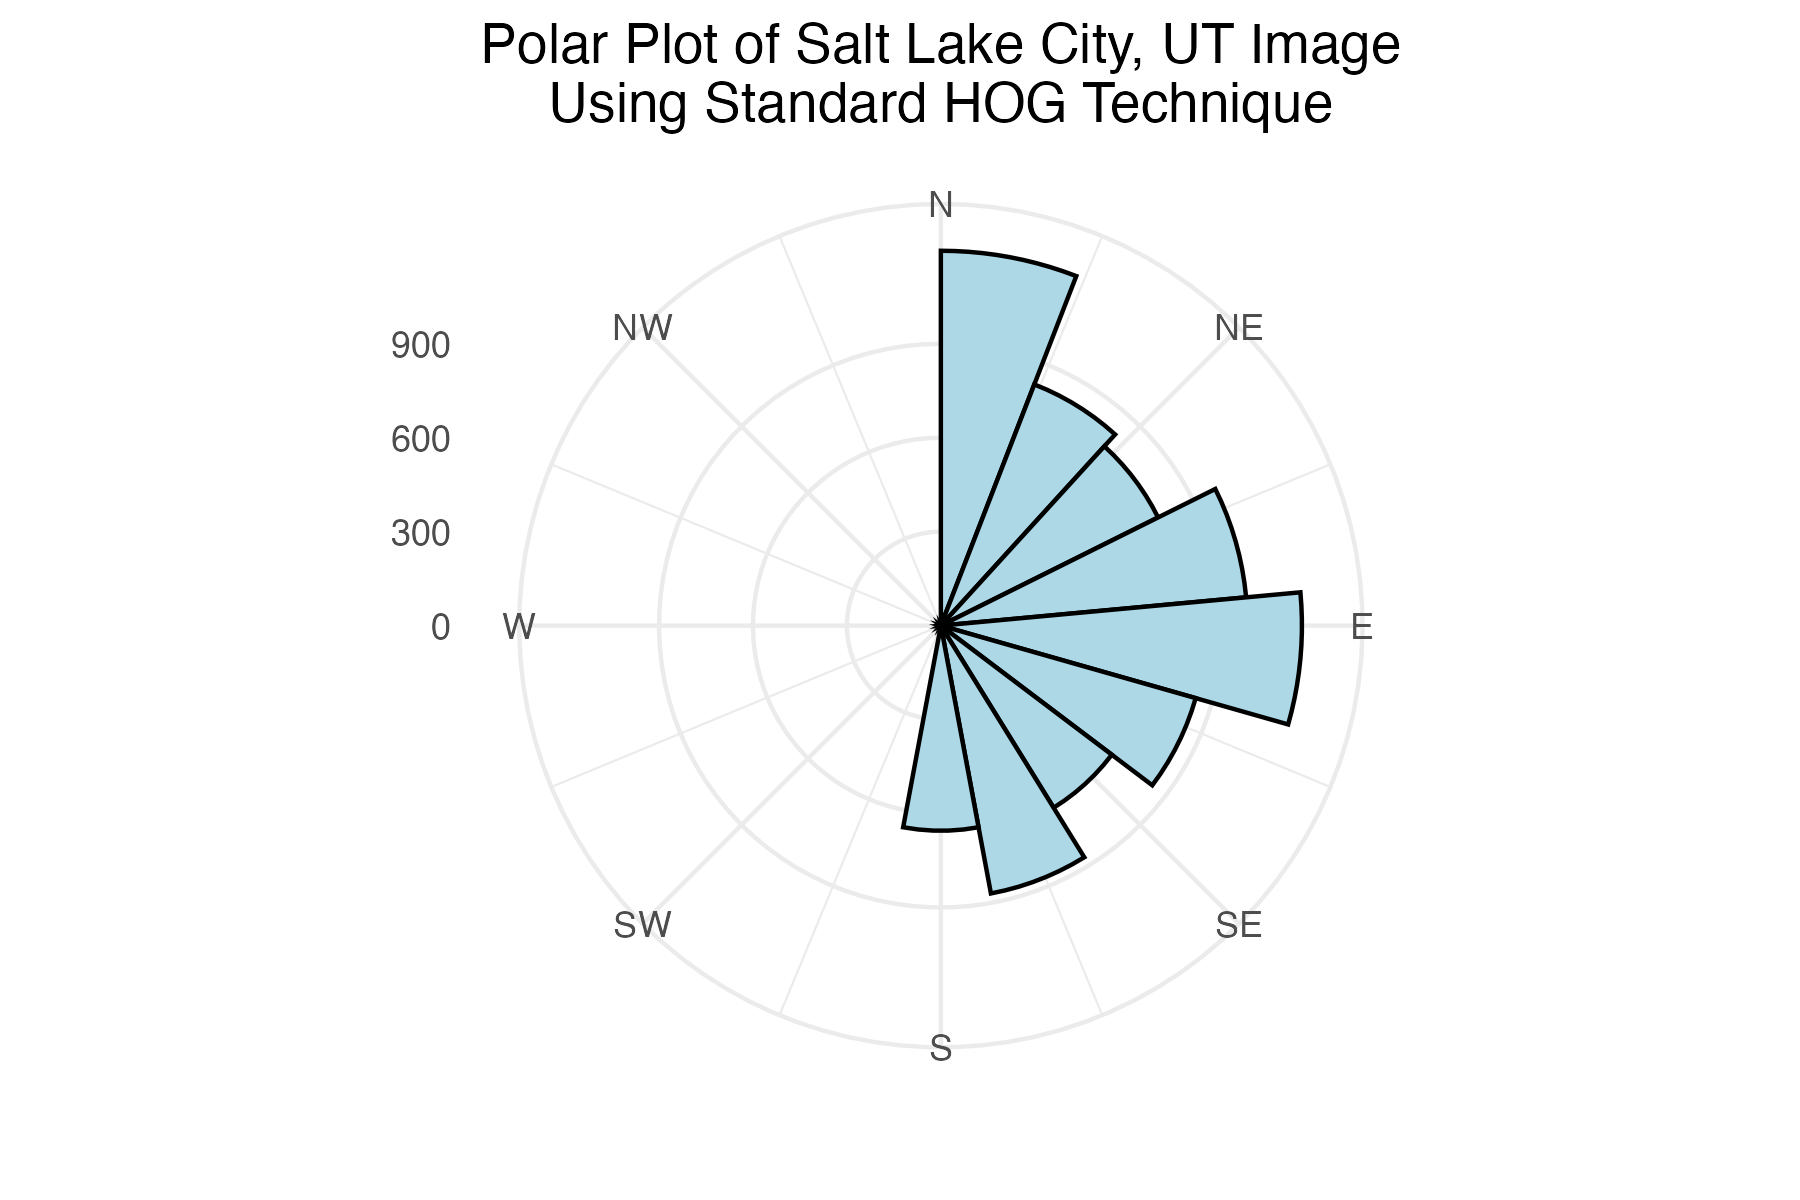
\includegraphics{images/plots/aerial_cities/salt_lake_standard_polar_plot.jpg}

}

\subcaption{Salt Lake City, UT}

\end{figure}%

\end{minipage}%
%
\begin{minipage}{0.33\linewidth}

\begin{figure}[H]

{\centering 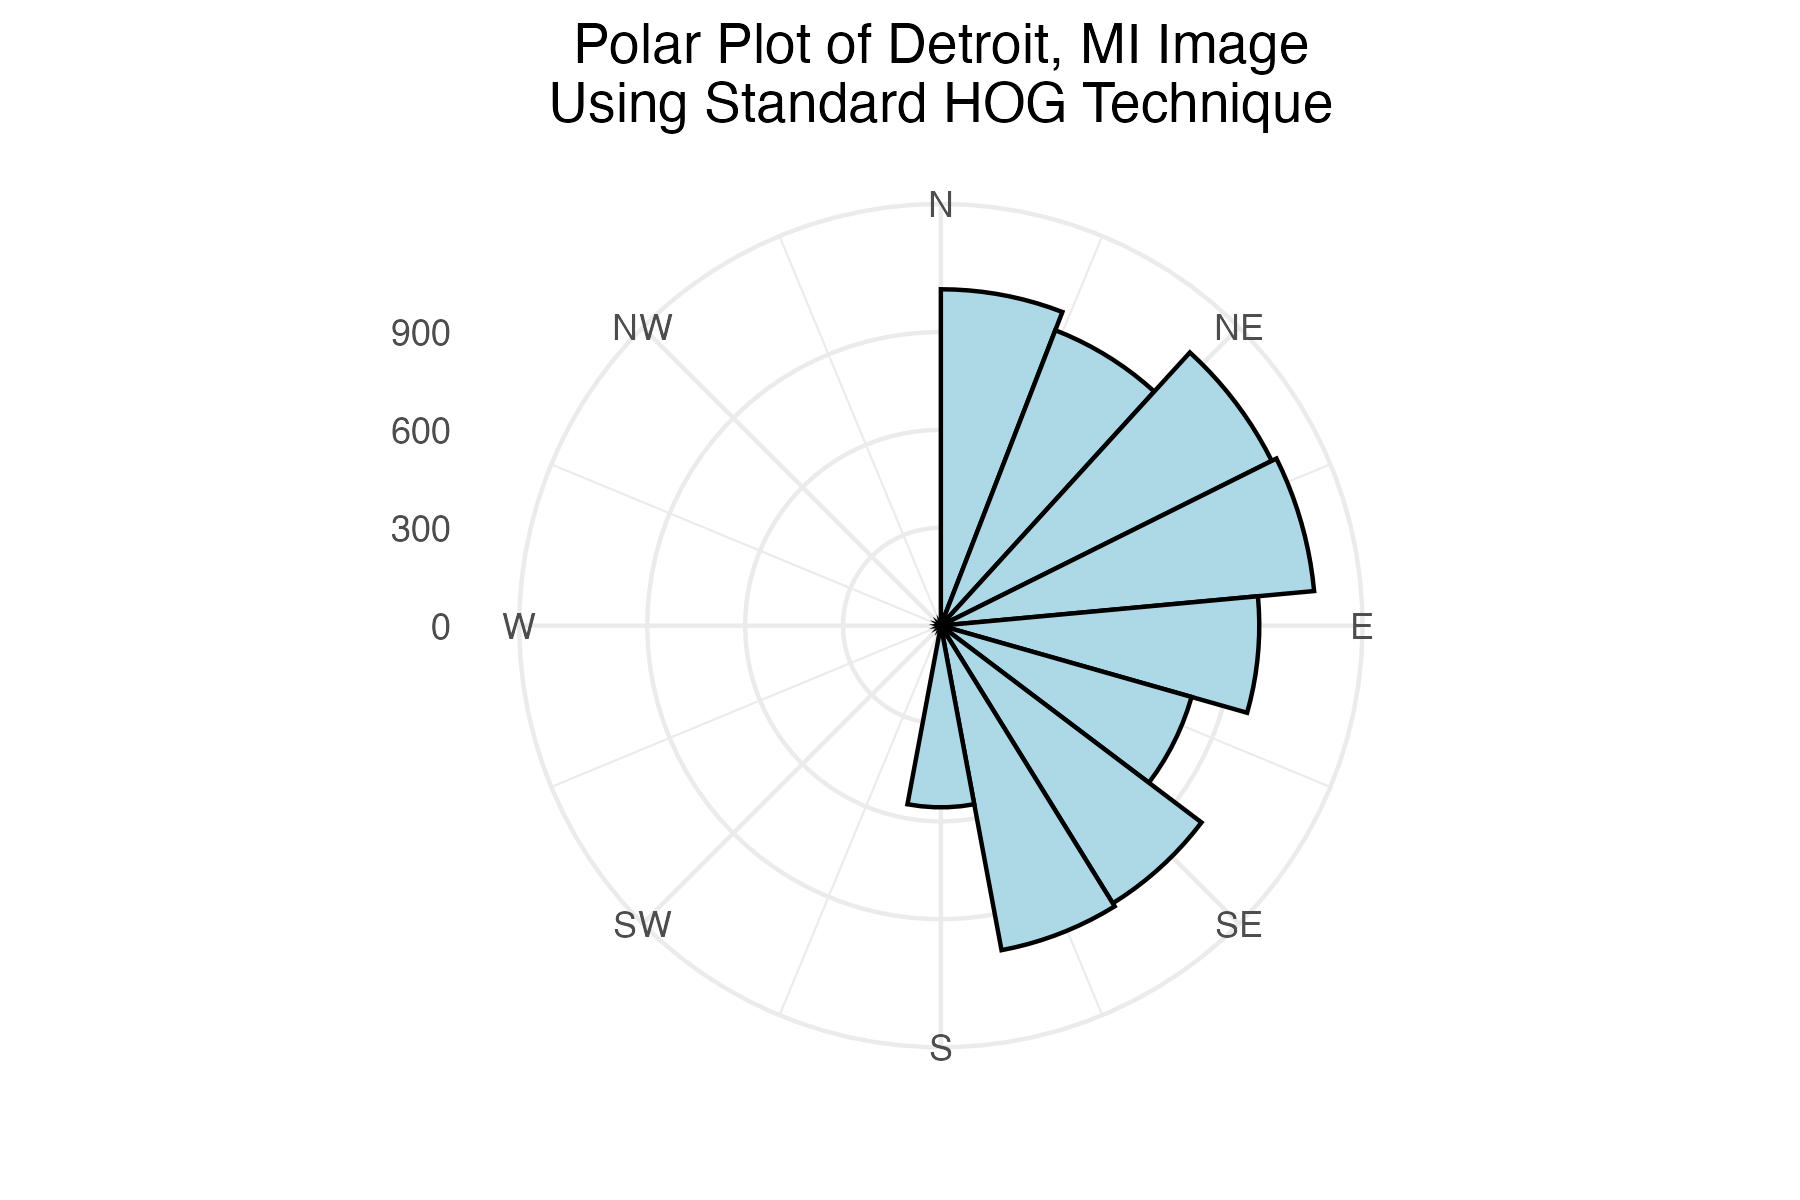
\includegraphics{images/plots/aerial_cities/detroit_standard_polar_plot.jpg}

}

\subcaption{Detroit, MI}

\end{figure}%

\end{minipage}%

\caption{\label{fig-city-standard-polar}Aerial Cityscape Standard Polar
Plots}

\end{figure}%

\section{Generate Polar Plots for Images Using Distributed Histogram
Binning
Technique}\label{generate-polar-plots-for-images-using-distributed-histogram-binning-technique}

\begin{Shaded}
\begin{Highlighting}[]
\CommentTok{\# SF plot}
\NormalTok{sf\_split\_plot }\OtherTok{\textless{}{-}}
  \FunctionTok{ggplot}\NormalTok{(aerial\_contribution\_df\_list[[}\DecValTok{1}\NormalTok{]], }
         \FunctionTok{aes}\NormalTok{(}\AttributeTok{x =}\NormalTok{ bin, }\AttributeTok{y =}\NormalTok{ contribution\_sum)) }\SpecialCharTok{+}
  \FunctionTok{geom\_histogram}\NormalTok{(}\AttributeTok{stat =} \StringTok{"identity"}\NormalTok{,}
                 \AttributeTok{colour =} \StringTok{"black"}\NormalTok{, }
                 \AttributeTok{fill =} \StringTok{"lightblue"}\NormalTok{, }
                 \AttributeTok{breaks =} \FunctionTok{seq}\NormalTok{(}\DecValTok{0}\NormalTok{, }\DecValTok{360}\NormalTok{, }\AttributeTok{length.out =} \FloatTok{17.5}\NormalTok{),}
                 \AttributeTok{bins =} \DecValTok{9}\NormalTok{) }\SpecialCharTok{+}
  \FunctionTok{coord\_polar}\NormalTok{(}
    \AttributeTok{theta =} \StringTok{"x"}\NormalTok{, }
    \AttributeTok{start =} \DecValTok{0}\NormalTok{, }
    \AttributeTok{direction =} \DecValTok{1}\NormalTok{) }\SpecialCharTok{+}
  \FunctionTok{scale\_x\_continuous}\NormalTok{(}\AttributeTok{limits =} \FunctionTok{c}\NormalTok{(}\DecValTok{0}\NormalTok{,}\DecValTok{360}\NormalTok{),}
    \AttributeTok{breaks =} \FunctionTok{c}\NormalTok{(}\DecValTok{0}\NormalTok{, }\DecValTok{45}\NormalTok{, }\DecValTok{90}\NormalTok{, }\DecValTok{135}\NormalTok{, }\DecValTok{180}\NormalTok{, }\DecValTok{225}\NormalTok{, }\DecValTok{270}\NormalTok{, }\DecValTok{315}\NormalTok{), }
    \AttributeTok{labels =} \FunctionTok{c}\NormalTok{(}\StringTok{"N"}\NormalTok{, }\StringTok{"NE"}\NormalTok{, }\StringTok{"E"}\NormalTok{, }\StringTok{"SE"}\NormalTok{, }\StringTok{"S"}\NormalTok{, }\StringTok{"SW"}\NormalTok{, }\StringTok{"W"}\NormalTok{, }\StringTok{"NW"}\NormalTok{)}
\NormalTok{  )}\SpecialCharTok{+}
  \FunctionTok{labs}\NormalTok{(}\AttributeTok{title =} \StringTok{"Polar Plot of San Francisco, CA Image}\SpecialCharTok{\textbackslash{}n}\StringTok{Using Distributed HOG Technique"}\NormalTok{) }\SpecialCharTok{+}
  \FunctionTok{theme\_minimal}\NormalTok{() }\SpecialCharTok{+}
  \FunctionTok{labs}\NormalTok{(}\AttributeTok{x =} \StringTok{""}\NormalTok{) }\SpecialCharTok{+}
  \FunctionTok{theme}\NormalTok{(}\AttributeTok{axis.title.y =} \FunctionTok{element\_blank}\NormalTok{(),}
        \AttributeTok{plot.title =} \FunctionTok{element\_text}\NormalTok{(}\AttributeTok{hjust =} \FloatTok{0.5}\NormalTok{))}

\CommentTok{\# save image}
\FunctionTok{ggsave}\NormalTok{(}\StringTok{"images/plots/aerial\_cities/sf\_contribution\_polar\_plot.jpg"}\NormalTok{, sf\_split\_plot, }\AttributeTok{width =} \DecValTok{6}\NormalTok{, }\AttributeTok{height =} \DecValTok{4}\NormalTok{, }\AttributeTok{dpi =} \DecValTok{300}\NormalTok{)}
\end{Highlighting}
\end{Shaded}

\begin{Shaded}
\begin{Highlighting}[]
\CommentTok{\# SLC plot}
\NormalTok{salt\_lake\_split\_plot }\OtherTok{\textless{}{-}}
  \FunctionTok{ggplot}\NormalTok{(aerial\_contribution\_df\_list[[}\DecValTok{2}\NormalTok{]], }
         \FunctionTok{aes}\NormalTok{(}\AttributeTok{x =}\NormalTok{ bin, }\AttributeTok{y =}\NormalTok{ contribution\_sum)) }\SpecialCharTok{+}
  \FunctionTok{geom\_histogram}\NormalTok{(}\AttributeTok{stat =} \StringTok{"identity"}\NormalTok{,}
                 \AttributeTok{colour =} \StringTok{"black"}\NormalTok{, }
                 \AttributeTok{fill =} \StringTok{"lightblue"}\NormalTok{, }
                 \AttributeTok{breaks =} \FunctionTok{seq}\NormalTok{(}\DecValTok{0}\NormalTok{, }\DecValTok{360}\NormalTok{, }\AttributeTok{length.out =} \FloatTok{17.5}\NormalTok{),}
                 \AttributeTok{bins =} \DecValTok{9}\NormalTok{) }\SpecialCharTok{+}
  \FunctionTok{coord\_polar}\NormalTok{(}
    \AttributeTok{theta =} \StringTok{"x"}\NormalTok{, }
    \AttributeTok{start =} \DecValTok{0}\NormalTok{, }
    \AttributeTok{direction =} \DecValTok{1}\NormalTok{) }\SpecialCharTok{+}
  \FunctionTok{scale\_x\_continuous}\NormalTok{(}\AttributeTok{limits =} \FunctionTok{c}\NormalTok{(}\DecValTok{0}\NormalTok{,}\DecValTok{360}\NormalTok{),}
    \AttributeTok{breaks =} \FunctionTok{c}\NormalTok{(}\DecValTok{0}\NormalTok{, }\DecValTok{45}\NormalTok{, }\DecValTok{90}\NormalTok{, }\DecValTok{135}\NormalTok{, }\DecValTok{180}\NormalTok{, }\DecValTok{225}\NormalTok{, }\DecValTok{270}\NormalTok{, }\DecValTok{315}\NormalTok{), }
    \AttributeTok{labels =} \FunctionTok{c}\NormalTok{(}\StringTok{"N"}\NormalTok{, }\StringTok{"NE"}\NormalTok{, }\StringTok{"E"}\NormalTok{, }\StringTok{"SE"}\NormalTok{, }\StringTok{"S"}\NormalTok{, }\StringTok{"SW"}\NormalTok{, }\StringTok{"W"}\NormalTok{, }\StringTok{"NW"}\NormalTok{)}
\NormalTok{  )}\SpecialCharTok{+}
  \FunctionTok{labs}\NormalTok{(}\AttributeTok{title =} \StringTok{"Polar Plot of Salt Lake City, UT Image}\SpecialCharTok{\textbackslash{}n}\StringTok{Using Distributed HOG Technique"}\NormalTok{) }\SpecialCharTok{+}
  \FunctionTok{theme\_minimal}\NormalTok{() }\SpecialCharTok{+}
  \FunctionTok{labs}\NormalTok{(}\AttributeTok{x =} \StringTok{""}\NormalTok{) }\SpecialCharTok{+}
  \FunctionTok{theme}\NormalTok{(}\AttributeTok{axis.title.y =} \FunctionTok{element\_blank}\NormalTok{(),}
        \AttributeTok{plot.title =} \FunctionTok{element\_text}\NormalTok{(}\AttributeTok{hjust =} \FloatTok{0.5}\NormalTok{))}

\CommentTok{\# save image}
\FunctionTok{ggsave}\NormalTok{(}\StringTok{"images/plots/aerial\_cities/salt\_lake\_contribution\_polar\_plot.jpg"}\NormalTok{, salt\_lake\_split\_plot, }\AttributeTok{width =} \DecValTok{6}\NormalTok{, }\AttributeTok{height =} \DecValTok{4}\NormalTok{, }\AttributeTok{dpi =} \DecValTok{300}\NormalTok{)}
\end{Highlighting}
\end{Shaded}

\begin{Shaded}
\begin{Highlighting}[]
\CommentTok{\# Detroit plot}
\NormalTok{detroit\_split\_plot }\OtherTok{\textless{}{-}}
  \FunctionTok{ggplot}\NormalTok{(aerial\_contribution\_df\_list[[}\DecValTok{3}\NormalTok{]], }
         \FunctionTok{aes}\NormalTok{(}\AttributeTok{x =}\NormalTok{ bin, }\AttributeTok{y =}\NormalTok{ contribution\_sum)) }\SpecialCharTok{+}
  \FunctionTok{geom\_histogram}\NormalTok{(}\AttributeTok{stat =} \StringTok{"identity"}\NormalTok{,}
                 \AttributeTok{colour =} \StringTok{"black"}\NormalTok{, }
                 \AttributeTok{fill =} \StringTok{"lightblue"}\NormalTok{, }
                 \AttributeTok{breaks =} \FunctionTok{seq}\NormalTok{(}\DecValTok{0}\NormalTok{, }\DecValTok{360}\NormalTok{, }\AttributeTok{length.out =} \FloatTok{17.5}\NormalTok{),}
                 \AttributeTok{bins =} \DecValTok{9}\NormalTok{) }\SpecialCharTok{+}
  \FunctionTok{coord\_polar}\NormalTok{(}
    \AttributeTok{theta =} \StringTok{"x"}\NormalTok{, }
    \AttributeTok{start =} \DecValTok{0}\NormalTok{, }
    \AttributeTok{direction =} \DecValTok{1}\NormalTok{) }\SpecialCharTok{+}
  \FunctionTok{scale\_x\_continuous}\NormalTok{(}\AttributeTok{limits =} \FunctionTok{c}\NormalTok{(}\DecValTok{0}\NormalTok{,}\DecValTok{360}\NormalTok{),}
    \AttributeTok{breaks =} \FunctionTok{c}\NormalTok{(}\DecValTok{0}\NormalTok{, }\DecValTok{45}\NormalTok{, }\DecValTok{90}\NormalTok{, }\DecValTok{135}\NormalTok{, }\DecValTok{180}\NormalTok{, }\DecValTok{225}\NormalTok{, }\DecValTok{270}\NormalTok{, }\DecValTok{315}\NormalTok{), }
    \AttributeTok{labels =} \FunctionTok{c}\NormalTok{(}\StringTok{"N"}\NormalTok{, }\StringTok{"NE"}\NormalTok{, }\StringTok{"E"}\NormalTok{, }\StringTok{"SE"}\NormalTok{, }\StringTok{"S"}\NormalTok{, }\StringTok{"SW"}\NormalTok{, }\StringTok{"W"}\NormalTok{, }\StringTok{"NW"}\NormalTok{)}
\NormalTok{  )}\SpecialCharTok{+}
  \FunctionTok{labs}\NormalTok{(}\AttributeTok{title =} \StringTok{"Polar Plot of Detroit, MI Image}\SpecialCharTok{\textbackslash{}n}\StringTok{Using Distributed HOG Technique"}\NormalTok{) }\SpecialCharTok{+}
  \FunctionTok{theme\_minimal}\NormalTok{() }\SpecialCharTok{+}
  \FunctionTok{labs}\NormalTok{(}\AttributeTok{x =} \StringTok{""}\NormalTok{) }\SpecialCharTok{+}
  \FunctionTok{theme}\NormalTok{(}\AttributeTok{axis.title.y =} \FunctionTok{element\_blank}\NormalTok{(),}
        \AttributeTok{plot.title =} \FunctionTok{element\_text}\NormalTok{(}\AttributeTok{hjust =} \FloatTok{0.5}\NormalTok{))}

\CommentTok{\# save image}
\FunctionTok{ggsave}\NormalTok{(}\StringTok{"images/plots/aerial\_cities/detroit\_contribution\_polar\_plot.jpg"}\NormalTok{, detroit\_split\_plot, }\AttributeTok{width =} \DecValTok{6}\NormalTok{, }\AttributeTok{height =} \DecValTok{4}\NormalTok{, }\AttributeTok{dpi =} \DecValTok{300}\NormalTok{)}
\end{Highlighting}
\end{Shaded}

\begin{Shaded}
\begin{Highlighting}[]
\CommentTok{\# Save to an arranged image}
\NormalTok{all\_aerial\_contribution\_plots }\OtherTok{\textless{}{-}}\NormalTok{ ggpubr}\SpecialCharTok{::}\FunctionTok{ggarrange}\NormalTok{(sf\_split\_plot, }
\NormalTok{                                                   salt\_lake\_split\_plot, }
\NormalTok{                                                   detroit\_split\_plot)}

\FunctionTok{ggsave}\NormalTok{(}\StringTok{"images/plots/aerial\_cities/all\_aerial\_contribution\_plots.jpg"}\NormalTok{, }
\NormalTok{       all\_aerial\_contribution\_plots, }
       \AttributeTok{width =} \DecValTok{7}\NormalTok{, }
       \AttributeTok{height =} \DecValTok{7}\NormalTok{)}
\end{Highlighting}
\end{Shaded}

\begin{figure}

\begin{minipage}{0.33\linewidth}

\begin{figure}[H]

{\centering 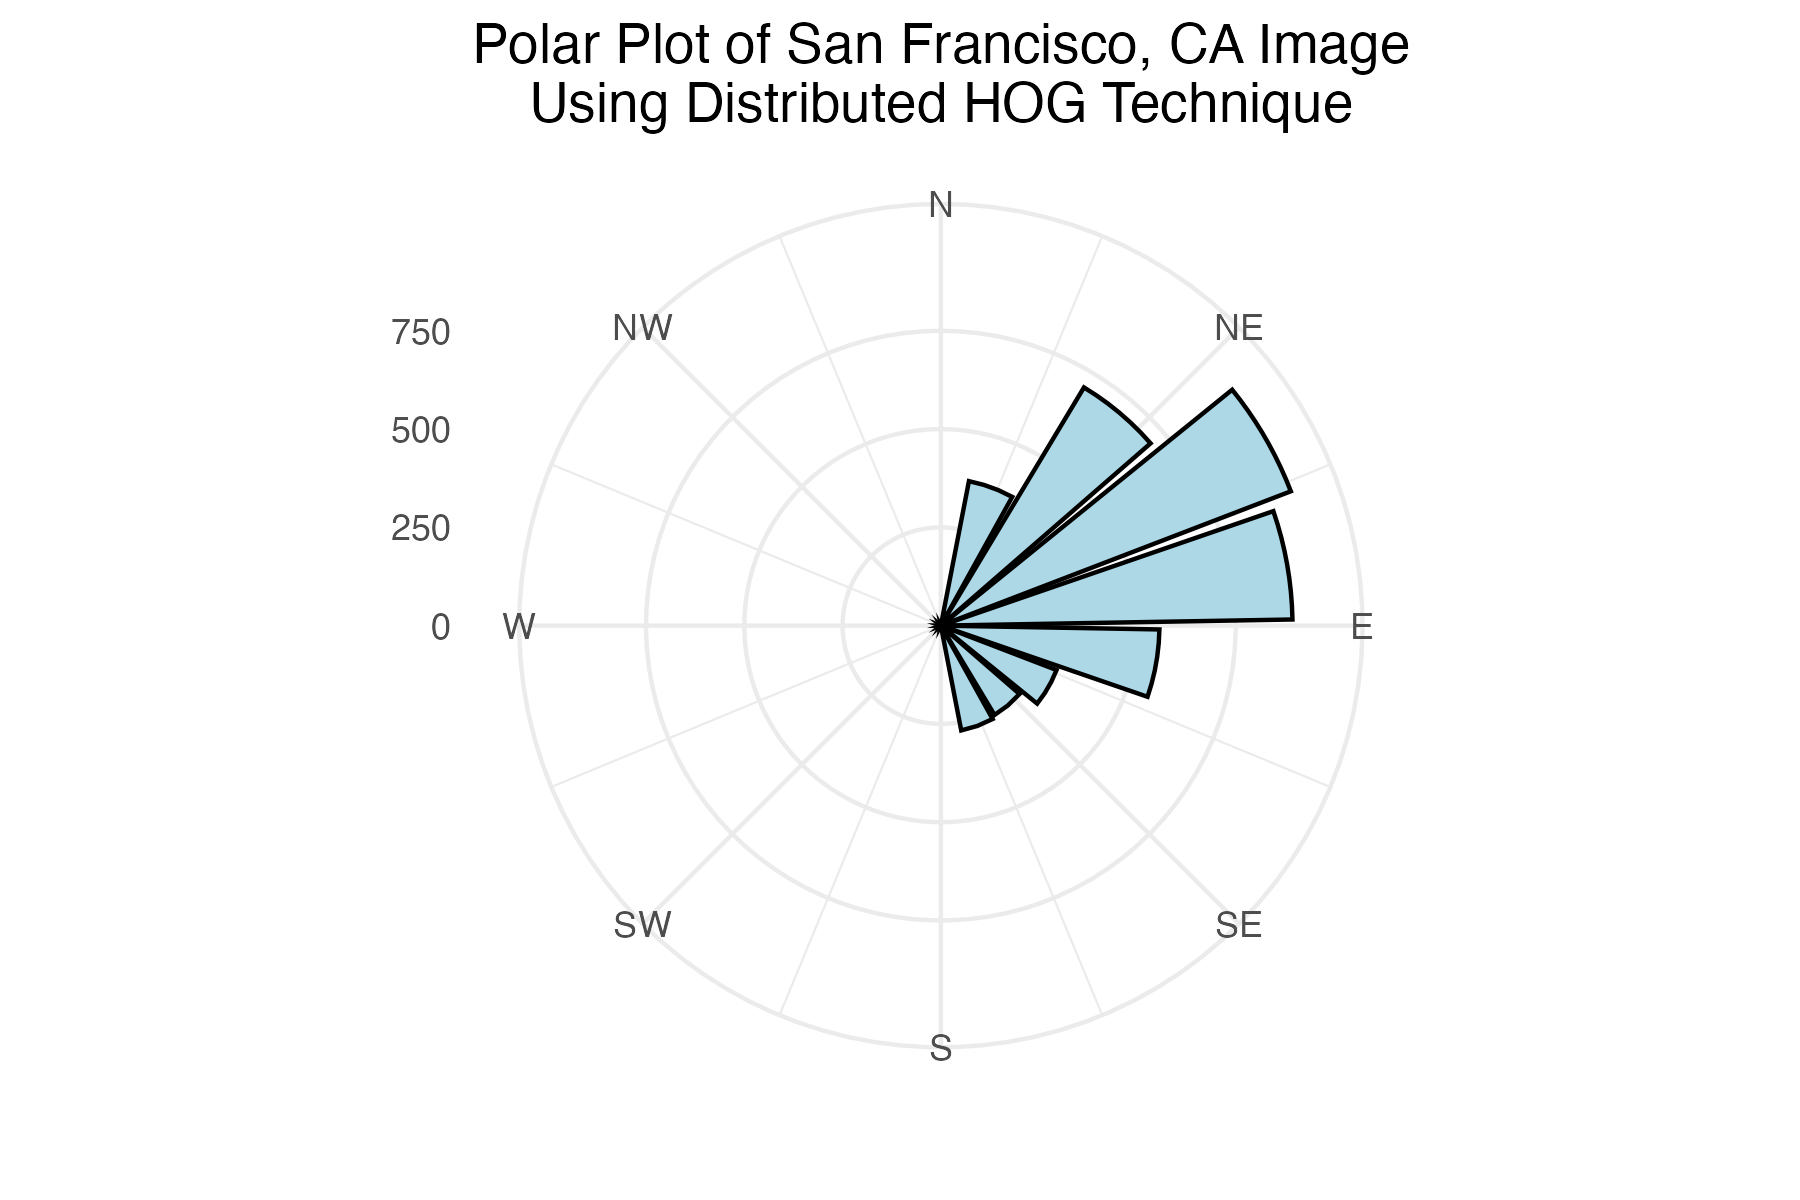
\includegraphics{images/plots/aerial_cities/sf_contribution_polar_plot.jpg}

}

\subcaption{San Francisco, CA}

\end{figure}%

\end{minipage}%
%
\begin{minipage}{0.33\linewidth}

\begin{figure}[H]

{\centering 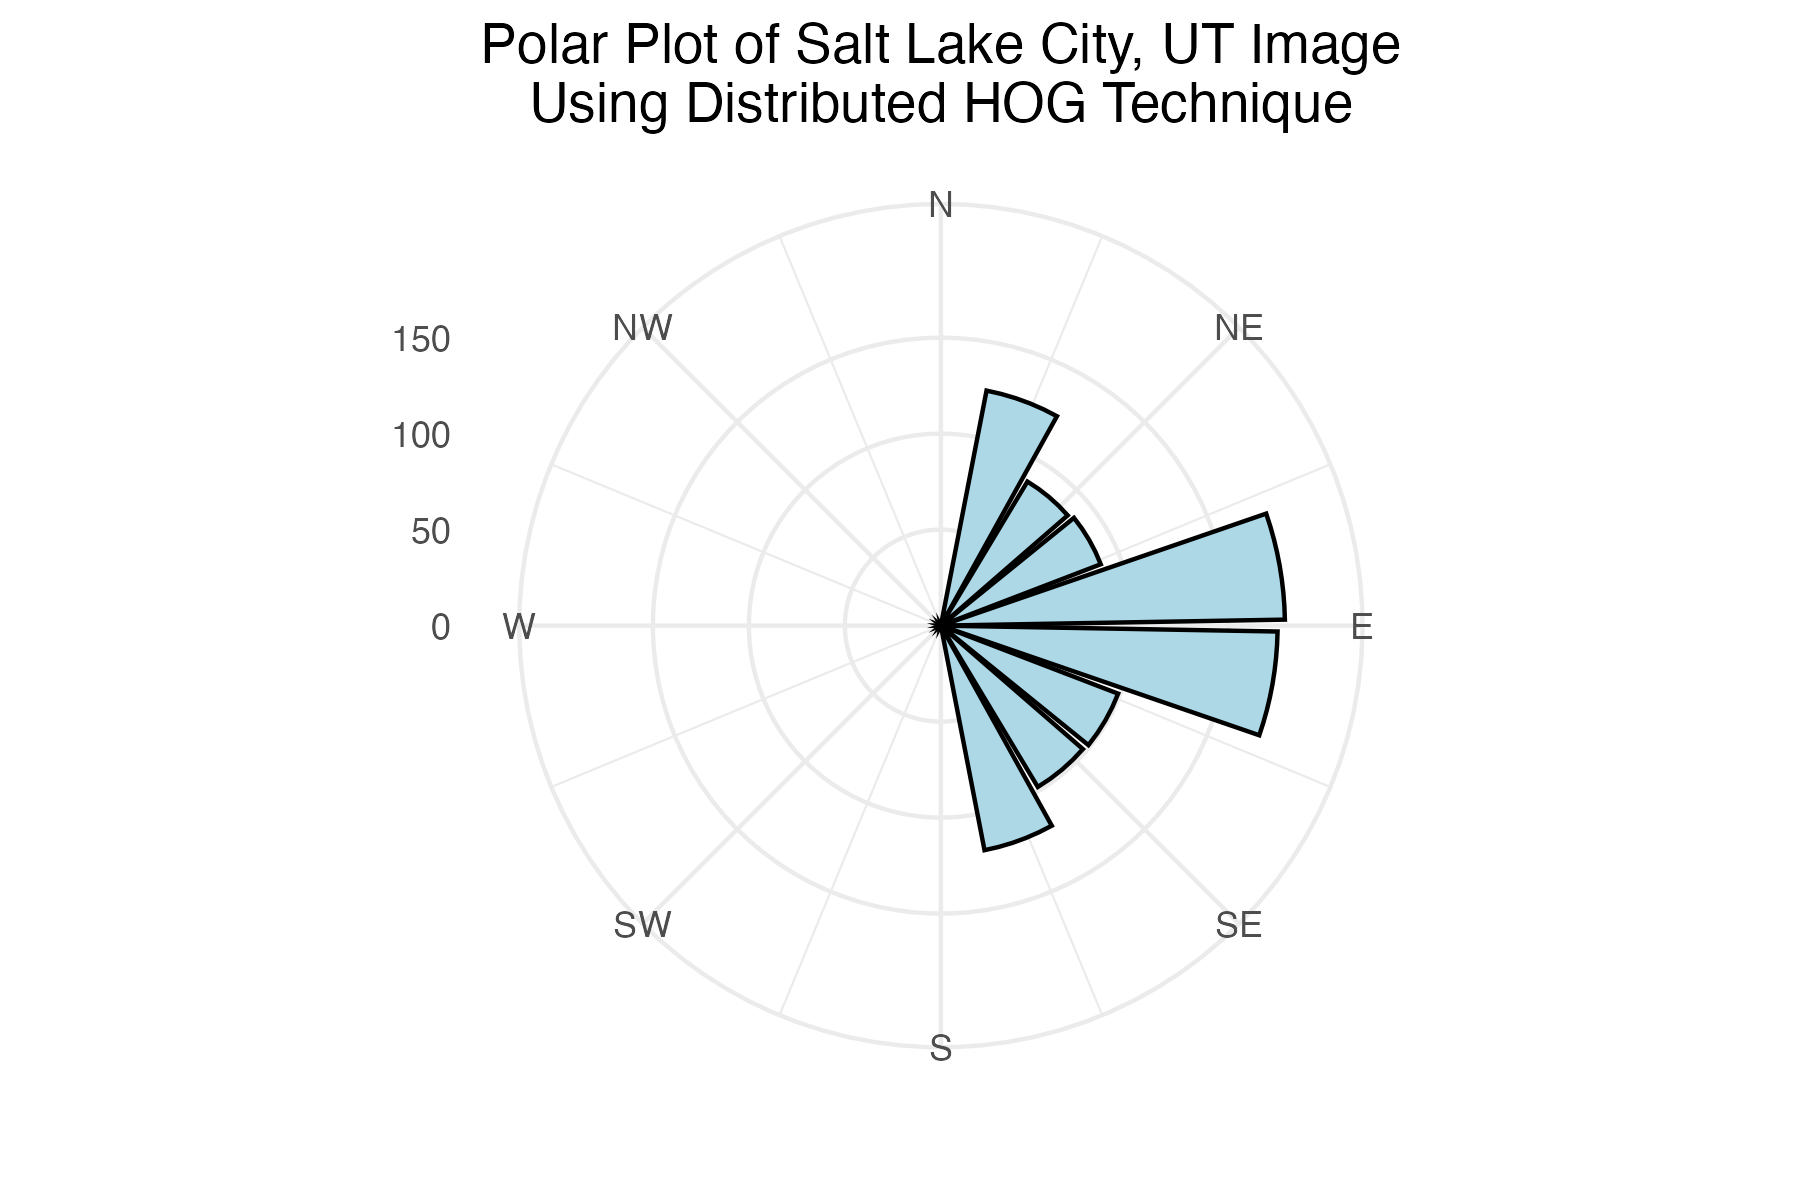
\includegraphics{images/plots/aerial_cities/salt_lake_contribution_polar_plot.jpg}

}

\subcaption{Salt Lake City, UT}

\end{figure}%

\end{minipage}%
%
\begin{minipage}{0.33\linewidth}

\begin{figure}[H]

{\centering 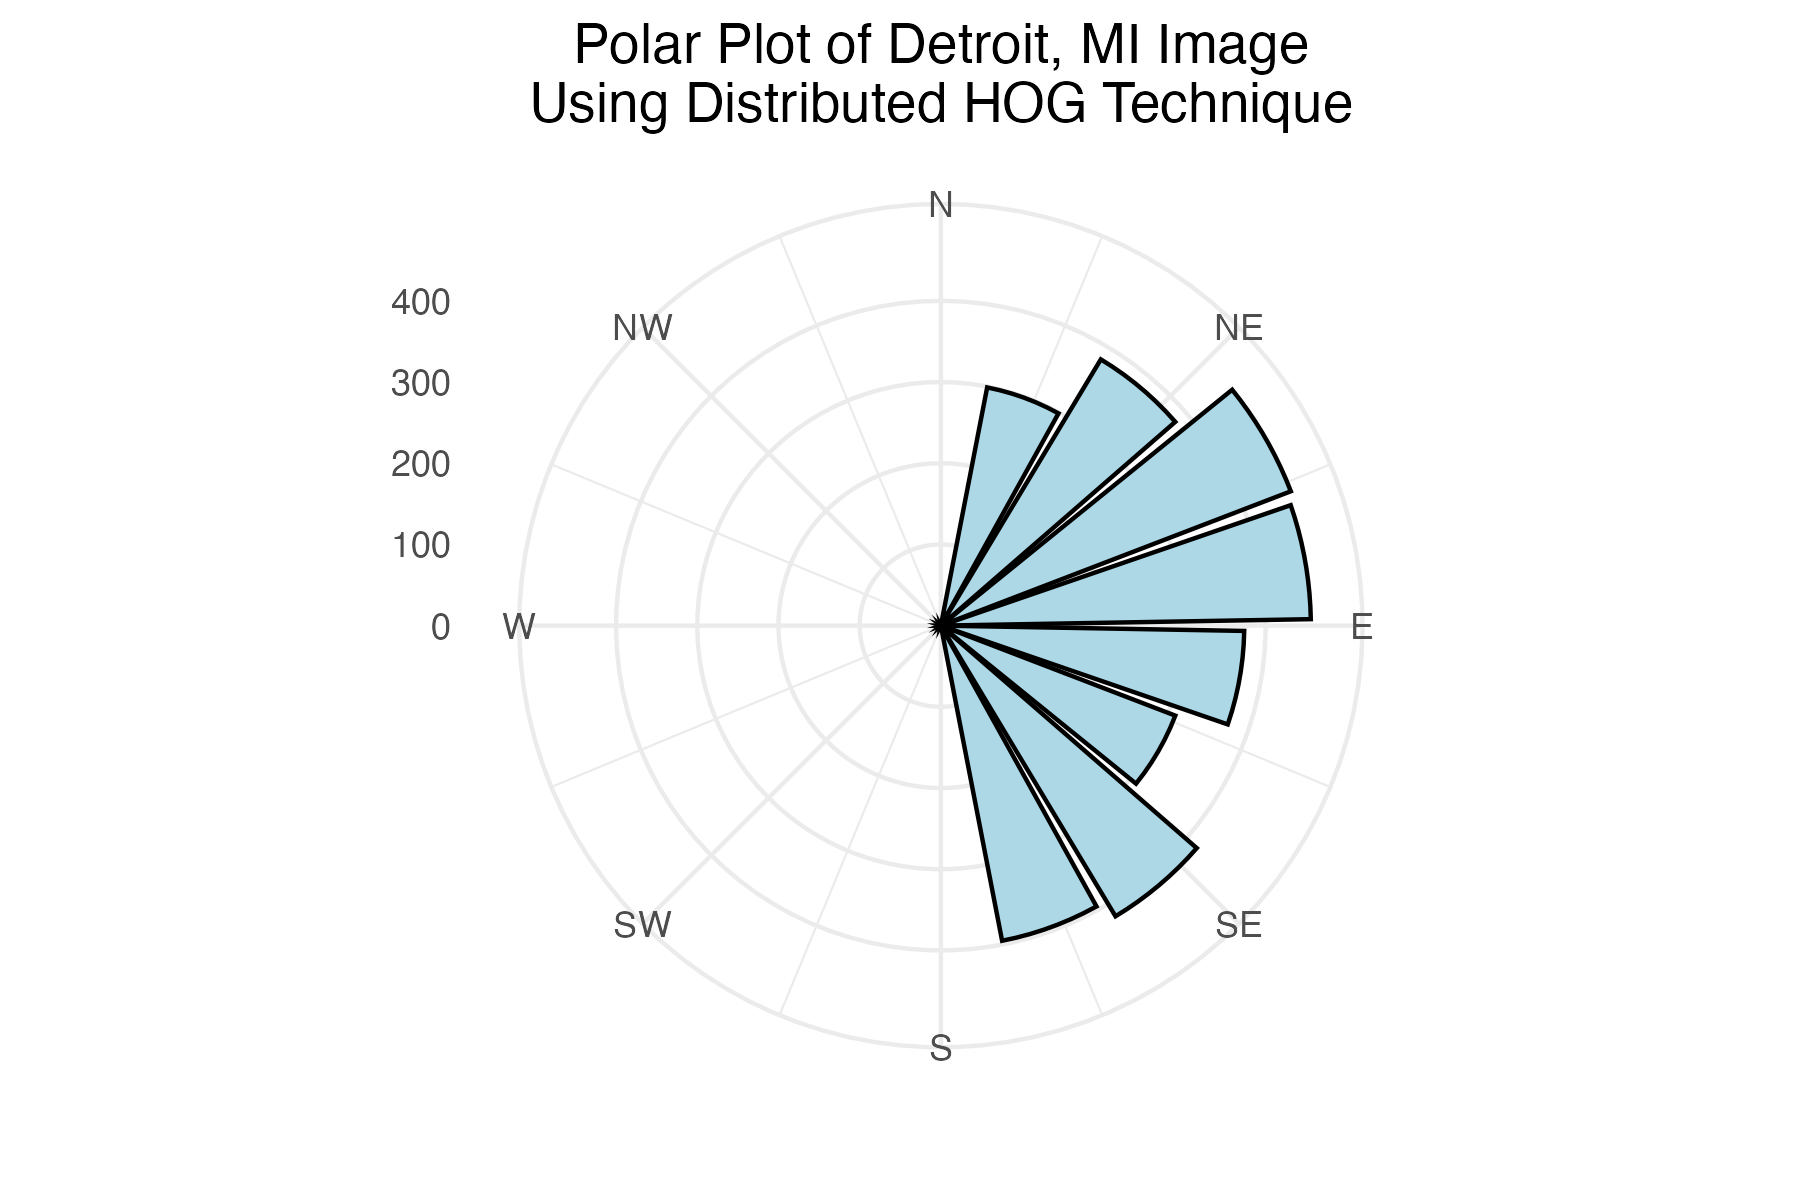
\includegraphics{images/plots/aerial_cities/detroit_contribution_polar_plot.jpg}

}

\subcaption{Detroit, MI}

\end{figure}%

\end{minipage}%

\caption{\label{fig-city-distributed-polar}Aerial Cityscape Distributed
Method Polar Plots}

\end{figure}%

\chapter{Grass Images}\label{grass-images}

\section{Load R Packages and Python
Libraries}\label{load-r-packages-and-python-libraries-1}

\begin{Shaded}
\begin{Highlighting}[]
\CommentTok{\# Load R Packages}
\FunctionTok{library}\NormalTok{(reticulate)}
\FunctionTok{library}\NormalTok{(tidyverse)}
\FunctionTok{library}\NormalTok{(mapsapi)}
\FunctionTok{library}\NormalTok{(mapboxapi)}
\FunctionTok{library}\NormalTok{(magick)}
\FunctionTok{Sys.which}\NormalTok{(}\StringTok{"python"}\NormalTok{)}
\end{Highlighting}
\end{Shaded}

\begin{verbatim}
                                                   python 
"/Users/bensunshine/.virtualenvs/r-reticulate/bin/python" 
\end{verbatim}

\begin{Shaded}
\begin{Highlighting}[]
\CommentTok{\# Load Python Libraries}
\ImportTok{import}\NormalTok{ matplotlib.pyplot }\ImportTok{as}\NormalTok{ plt}
\ImportTok{import}\NormalTok{ pandas }\ImportTok{as}\NormalTok{ pd}
\ImportTok{from}\NormalTok{ skimage.io }\ImportTok{import}\NormalTok{ imread, imshow}
\ImportTok{from}\NormalTok{ skimage.transform }\ImportTok{import}\NormalTok{ resize}
\ImportTok{from}\NormalTok{ skimage.feature }\ImportTok{import}\NormalTok{ hog}
\ImportTok{from}\NormalTok{ skimage }\ImportTok{import}\NormalTok{ data, exposure}
\ImportTok{import}\NormalTok{ matplotlib.pyplot }\ImportTok{as}\NormalTok{ plt}
\ImportTok{from}\NormalTok{ skimage }\ImportTok{import}\NormalTok{ io}
\ImportTok{from}\NormalTok{ skimage }\ImportTok{import}\NormalTok{ color}
\ImportTok{from}\NormalTok{ skimage.transform }\ImportTok{import}\NormalTok{ resize}
\ImportTok{import}\NormalTok{ math}
\ImportTok{from}\NormalTok{ skimage.feature }\ImportTok{import}\NormalTok{ hog}
\ImportTok{import}\NormalTok{ numpy }\ImportTok{as}\NormalTok{ np}
\end{Highlighting}
\end{Shaded}

\section{Collect HOG Features for Grass
Images}\label{collect-hog-features-for-grass-images}

\begin{Shaded}
\begin{Highlighting}[]
\CommentTok{\# List for storing images}
\NormalTok{img\_list }\OperatorTok{=}\NormalTok{ []}

\CommentTok{\# Internet Grass Image}
\NormalTok{img\_list.append(color.rgb2gray(io.imread(}\StringTok{"images/grass\_image2.jpg"}\NormalTok{)))}

\CommentTok{\# Living Labs Rotated Aerial Grass}
\NormalTok{img\_list.append(color.rgb2gray(io.imread(}\StringTok{"images/living\_lab\_aerial/aerial\_grass\_living\_lab\_rotated.jpg"}\NormalTok{)))}

\CommentTok{\# Living Labs Grass Close{-}up}
\NormalTok{img\_list.append(color.rgb2gray(io.imread(}\StringTok{"images/living\_lab\_aerial/LL\_zoomed\_in\_12.jpg"}\NormalTok{)))}

\CommentTok{\# List to store magnitudes for each image}
\NormalTok{mag\_list }\OperatorTok{=}\NormalTok{ []}

\CommentTok{\# List to store angles for each image}
\NormalTok{theta\_list }\OperatorTok{=}\NormalTok{ []}


\ControlFlowTok{for}\NormalTok{ x }\KeywordTok{in} \BuiltInTok{range}\NormalTok{(}\BuiltInTok{len}\NormalTok{(img\_list)):}
    \CommentTok{\# Get image of interest}
\NormalTok{    img }\OperatorTok{=}\NormalTok{ img\_list[x]}
    
\NormalTok{    rescaled\_file\_path }\OperatorTok{=} \SpecialStringTok{f"images/plots/grass/}\SpecialCharTok{\{}\NormalTok{x}\SpecialCharTok{\}}\SpecialStringTok{.jpg"}
    
    \CommentTok{\# Determine aspect Ratio}
\NormalTok{    aspect\_ratio }\OperatorTok{=}\NormalTok{ img.shape[}\DecValTok{0}\NormalTok{] }\OperatorTok{/}\NormalTok{ img.shape[}\DecValTok{1}\NormalTok{]}
    \BuiltInTok{print}\NormalTok{(}\StringTok{"Aspect Ratio:"}\NormalTok{, aspect\_ratio)}
    
    \CommentTok{\# Hard{-}Code height to 200 pixels}
\NormalTok{    height }\OperatorTok{=} \DecValTok{200}
    
    \CommentTok{\# Calculate witdth to maintain same aspect ratio}
\NormalTok{    width }\OperatorTok{=} \BuiltInTok{int}\NormalTok{(height }\OperatorTok{/}\NormalTok{ aspect\_ratio)}
    \BuiltInTok{print}\NormalTok{(}\StringTok{"Resized Width:"}\NormalTok{, width)}
    
    \CommentTok{\# Resize the image}
\NormalTok{    resized\_img }\OperatorTok{=}\NormalTok{ resize(img, (height, width))}
    
    \CommentTok{\# Replace the original image with the resized image}
\NormalTok{    img\_list[x] }\OperatorTok{=}\NormalTok{ resized\_img}
    
    \CommentTok{\# plt.figure(figsize=(plot\_width, plot\_height))}
    \CommentTok{\# plt.imshow(resized\_img, cmap="gray")}
    \CommentTok{\# plt.axis("on")}
    \CommentTok{\# plt.tight\_layout()}
    \CommentTok{\# plt.savefig(rescaled\_file\_path, dpi=300)}
    \CommentTok{\# plt.show()}

    
    \CommentTok{\# list for storing all magnitudes for image[x]}
\NormalTok{    mag }\OperatorTok{=}\NormalTok{ []}
    
    \CommentTok{\# list for storing all angles for image[x]}
\NormalTok{    theta }\OperatorTok{=}\NormalTok{ []}
    
    \ControlFlowTok{for}\NormalTok{ i }\KeywordTok{in} \BuiltInTok{range}\NormalTok{(height):}
\NormalTok{        magnitudeArray }\OperatorTok{=}\NormalTok{ []}
\NormalTok{        angleArray }\OperatorTok{=}\NormalTok{ []}

        \ControlFlowTok{for}\NormalTok{ j }\KeywordTok{in} \BuiltInTok{range}\NormalTok{(width):}
            \ControlFlowTok{if}\NormalTok{ j }\OperatorTok{{-}} \DecValTok{1} \OperatorTok{\textless{}} \DecValTok{0} \KeywordTok{or}\NormalTok{ j }\OperatorTok{+} \DecValTok{1} \OperatorTok{\textgreater{}=}\NormalTok{ width:}
                \ControlFlowTok{if}\NormalTok{ j }\OperatorTok{{-}} \DecValTok{1} \OperatorTok{\textless{}} \DecValTok{0}\NormalTok{:}
\NormalTok{                    Gx }\OperatorTok{=}\NormalTok{ resized\_img[i][j }\OperatorTok{+} \DecValTok{1}\NormalTok{] }\OperatorTok{{-}} \DecValTok{0}
                \ControlFlowTok{elif}\NormalTok{ j }\OperatorTok{+} \DecValTok{1} \OperatorTok{\textgreater{}=}\NormalTok{ width:}
\NormalTok{                    Gx }\OperatorTok{=} \DecValTok{0} \OperatorTok{{-}}\NormalTok{ resized\_img[i][j }\OperatorTok{{-}} \DecValTok{1}\NormalTok{]}
            \ControlFlowTok{else}\NormalTok{:}
\NormalTok{                Gx }\OperatorTok{=}\NormalTok{ resized\_img[i][j }\OperatorTok{+} \DecValTok{1}\NormalTok{] }\OperatorTok{{-}}\NormalTok{ resized\_img[i][j }\OperatorTok{{-}} \DecValTok{1}\NormalTok{]}

            \ControlFlowTok{if}\NormalTok{ i }\OperatorTok{{-}} \DecValTok{1} \OperatorTok{\textless{}} \DecValTok{0} \KeywordTok{or}\NormalTok{ i }\OperatorTok{+} \DecValTok{1} \OperatorTok{\textgreater{}=}\NormalTok{ height:}
                \ControlFlowTok{if}\NormalTok{ i }\OperatorTok{{-}} \DecValTok{1} \OperatorTok{\textless{}} \DecValTok{0}\NormalTok{:}
\NormalTok{                    Gy }\OperatorTok{=} \DecValTok{0} \OperatorTok{{-}}\NormalTok{ resized\_img[i }\OperatorTok{+} \DecValTok{1}\NormalTok{][j]}
                \ControlFlowTok{elif}\NormalTok{ i }\OperatorTok{+} \DecValTok{1} \OperatorTok{\textgreater{}=}\NormalTok{ height:}
\NormalTok{                    Gy }\OperatorTok{=}\NormalTok{ resized\_img[i }\OperatorTok{{-}} \DecValTok{1}\NormalTok{][j] }\OperatorTok{{-}} \DecValTok{0}
            \ControlFlowTok{else}\NormalTok{:}
\NormalTok{                Gy }\OperatorTok{=}\NormalTok{ resized\_img[i }\OperatorTok{+} \DecValTok{1}\NormalTok{][j] }\OperatorTok{{-}}\NormalTok{ resized\_img[i }\OperatorTok{{-}} \DecValTok{1}\NormalTok{][j]}

\NormalTok{            magnitude }\OperatorTok{=}\NormalTok{ math.sqrt(}\BuiltInTok{pow}\NormalTok{(Gx, }\DecValTok{2}\NormalTok{) }\OperatorTok{+} \BuiltInTok{pow}\NormalTok{(Gy, }\DecValTok{2}\NormalTok{))}
\NormalTok{            magnitudeArray.append(}\BuiltInTok{round}\NormalTok{(magnitude, }\DecValTok{9}\NormalTok{))}

            \ControlFlowTok{if}\NormalTok{ Gx }\OperatorTok{==} \DecValTok{0}\NormalTok{:}
\NormalTok{                angle }\OperatorTok{=}\NormalTok{ math.degrees(}\FloatTok{0.0}\NormalTok{)}
            \ControlFlowTok{else}\NormalTok{:}
\NormalTok{                angle }\OperatorTok{=}\NormalTok{ math.degrees(math.atan(Gy }\OperatorTok{/}\NormalTok{ Gx))}
                \ControlFlowTok{if}\NormalTok{ angle }\OperatorTok{\textless{}} \DecValTok{0}\NormalTok{:}
\NormalTok{                    angle }\OperatorTok{+=} \DecValTok{180}

\NormalTok{            angleArray.append(}\BuiltInTok{round}\NormalTok{(angle, }\DecValTok{9}\NormalTok{))}

\NormalTok{        mag.append(magnitudeArray)}
\NormalTok{        theta.append(angleArray)}

    \CommentTok{\# add list of magnitudes to list[x]}
\NormalTok{    mag\_list.append(mag)}

    \CommentTok{\# add list of angles to angle list[x]}
\NormalTok{    theta\_list.append(theta)}
\end{Highlighting}
\end{Shaded}

\begin{verbatim}
Aspect Ratio: 0.662751677852349
Resized Width: 301
Aspect Ratio: 0.4904214559386973
Resized Width: 407
Aspect Ratio: 0.5625
Resized Width: 355
\end{verbatim}

\begin{figure}

\begin{minipage}{0.33\linewidth}

\begin{figure}[H]

{\centering 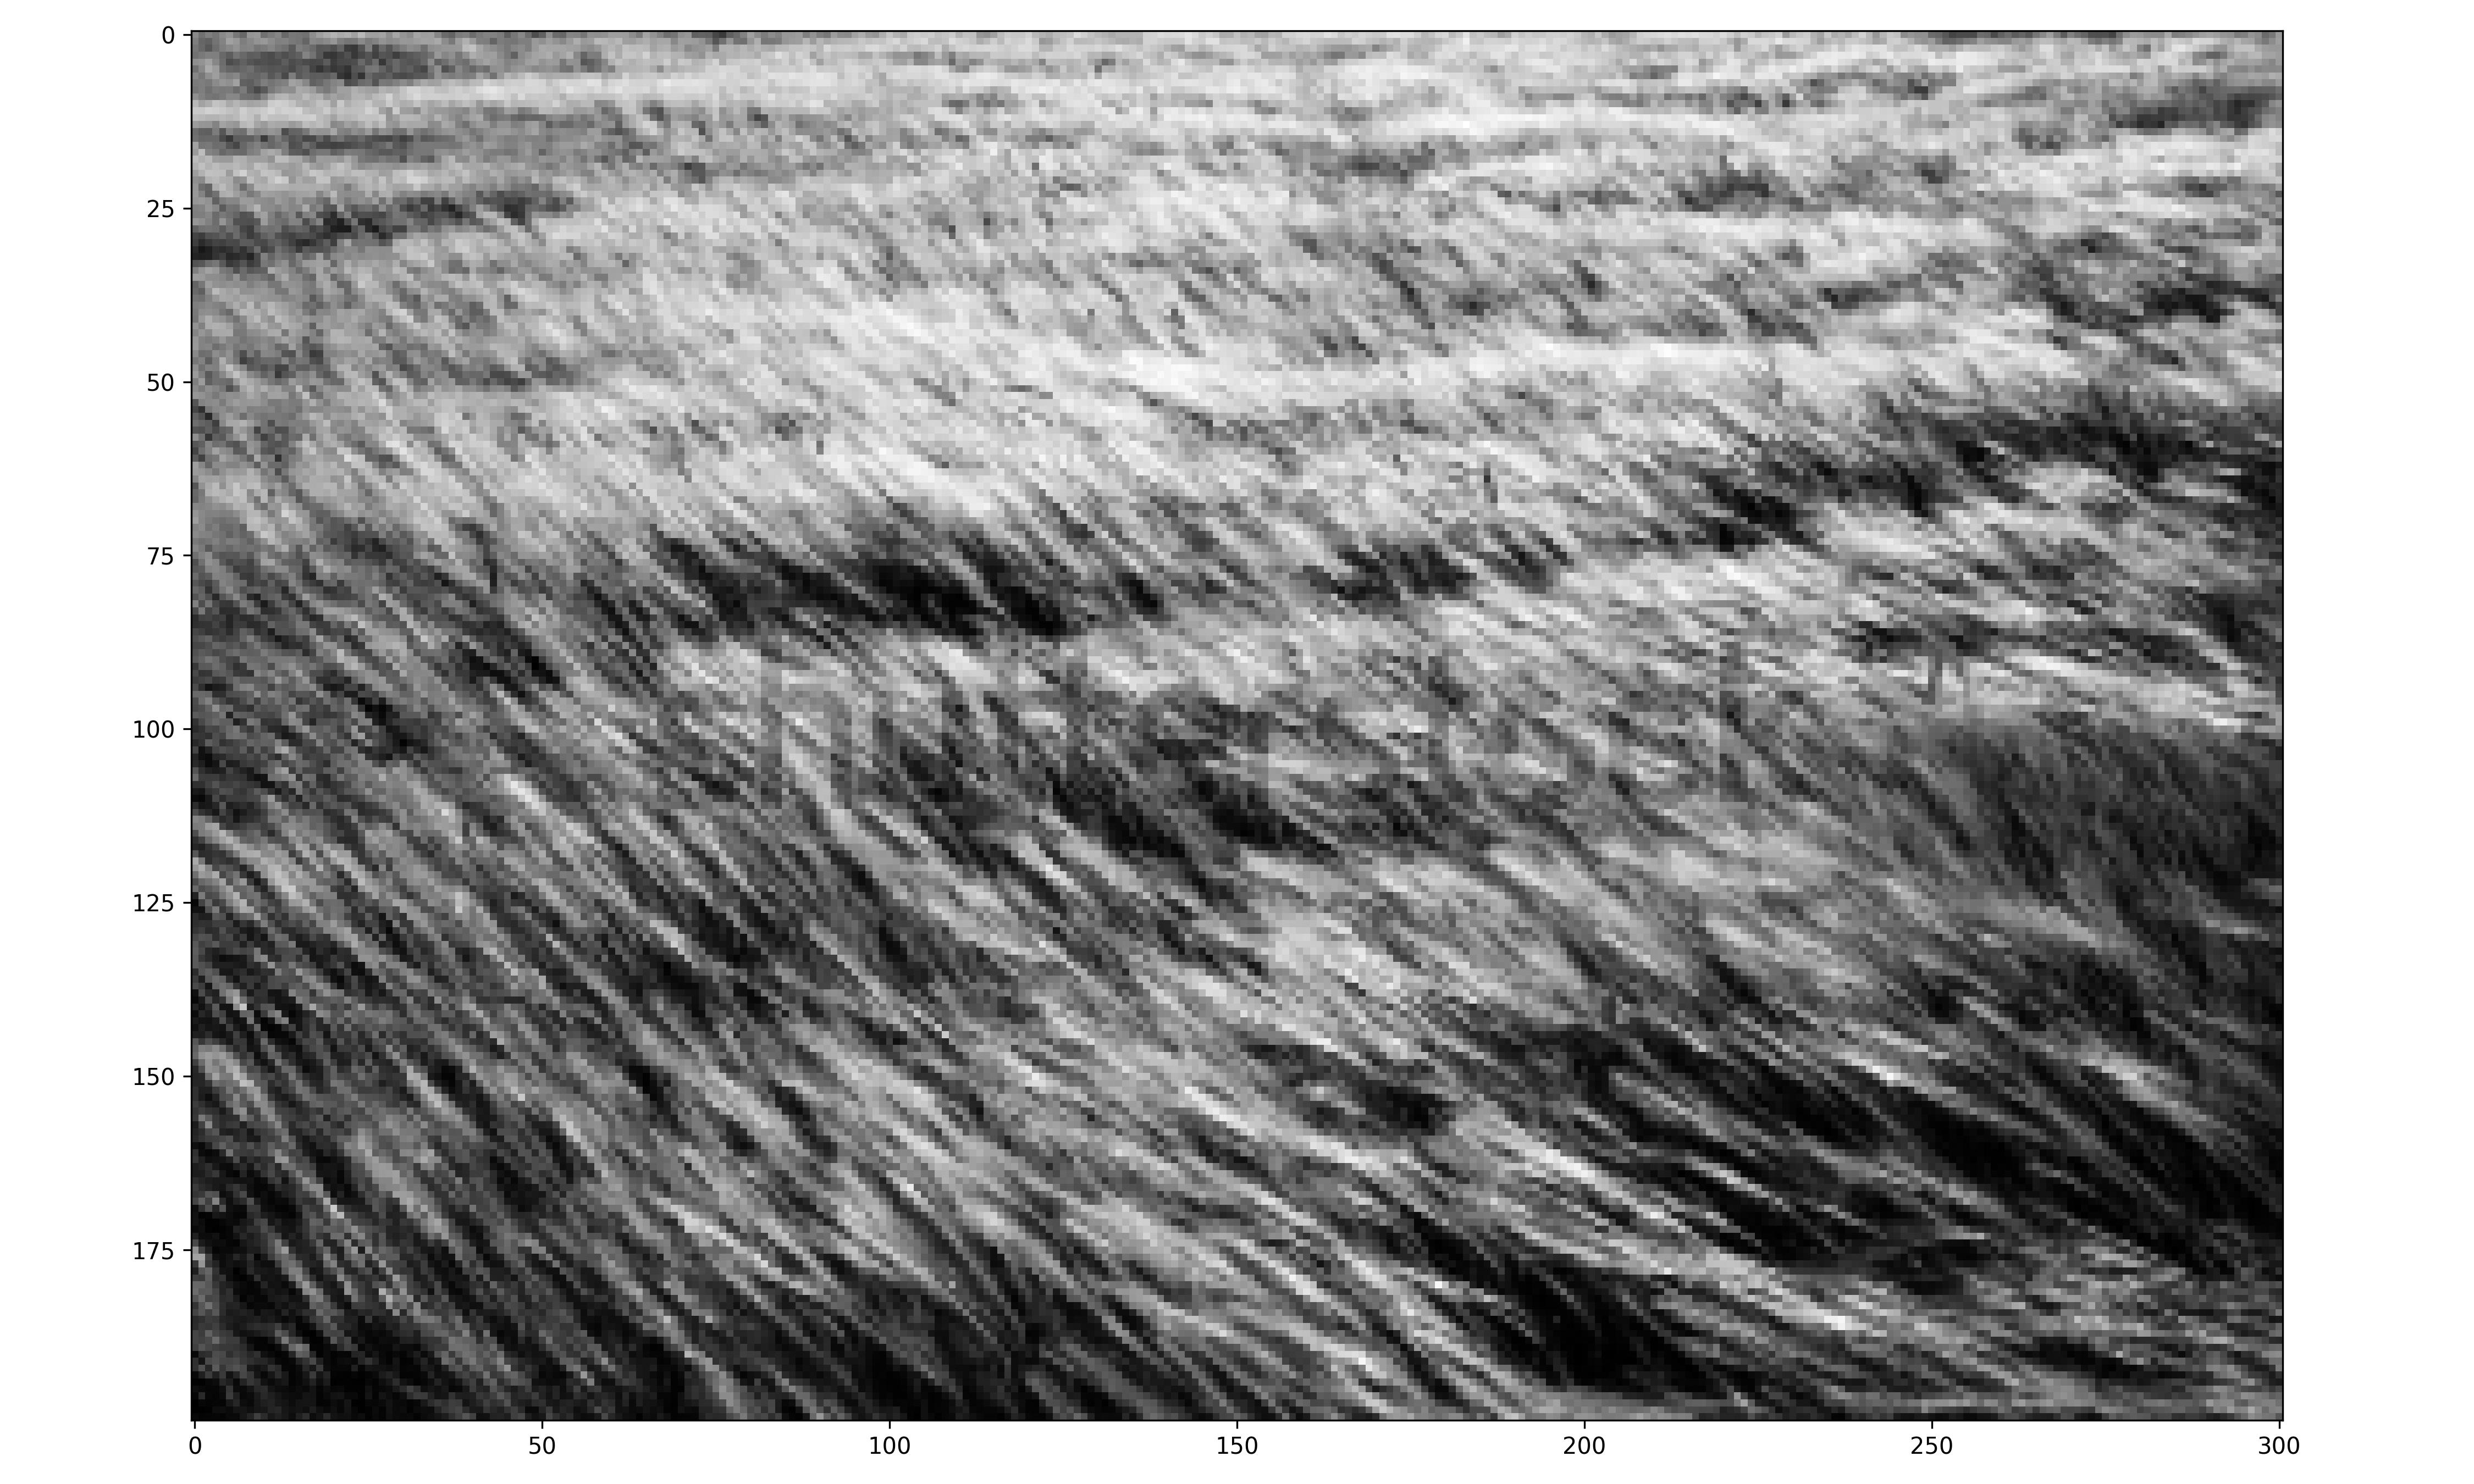
\includegraphics{images/plots/grass/0.jpg}

}

\subcaption{Internet Grass Image}

\end{figure}%

\end{minipage}%
%
\begin{minipage}{0.33\linewidth}

\begin{figure}[H]

{\centering 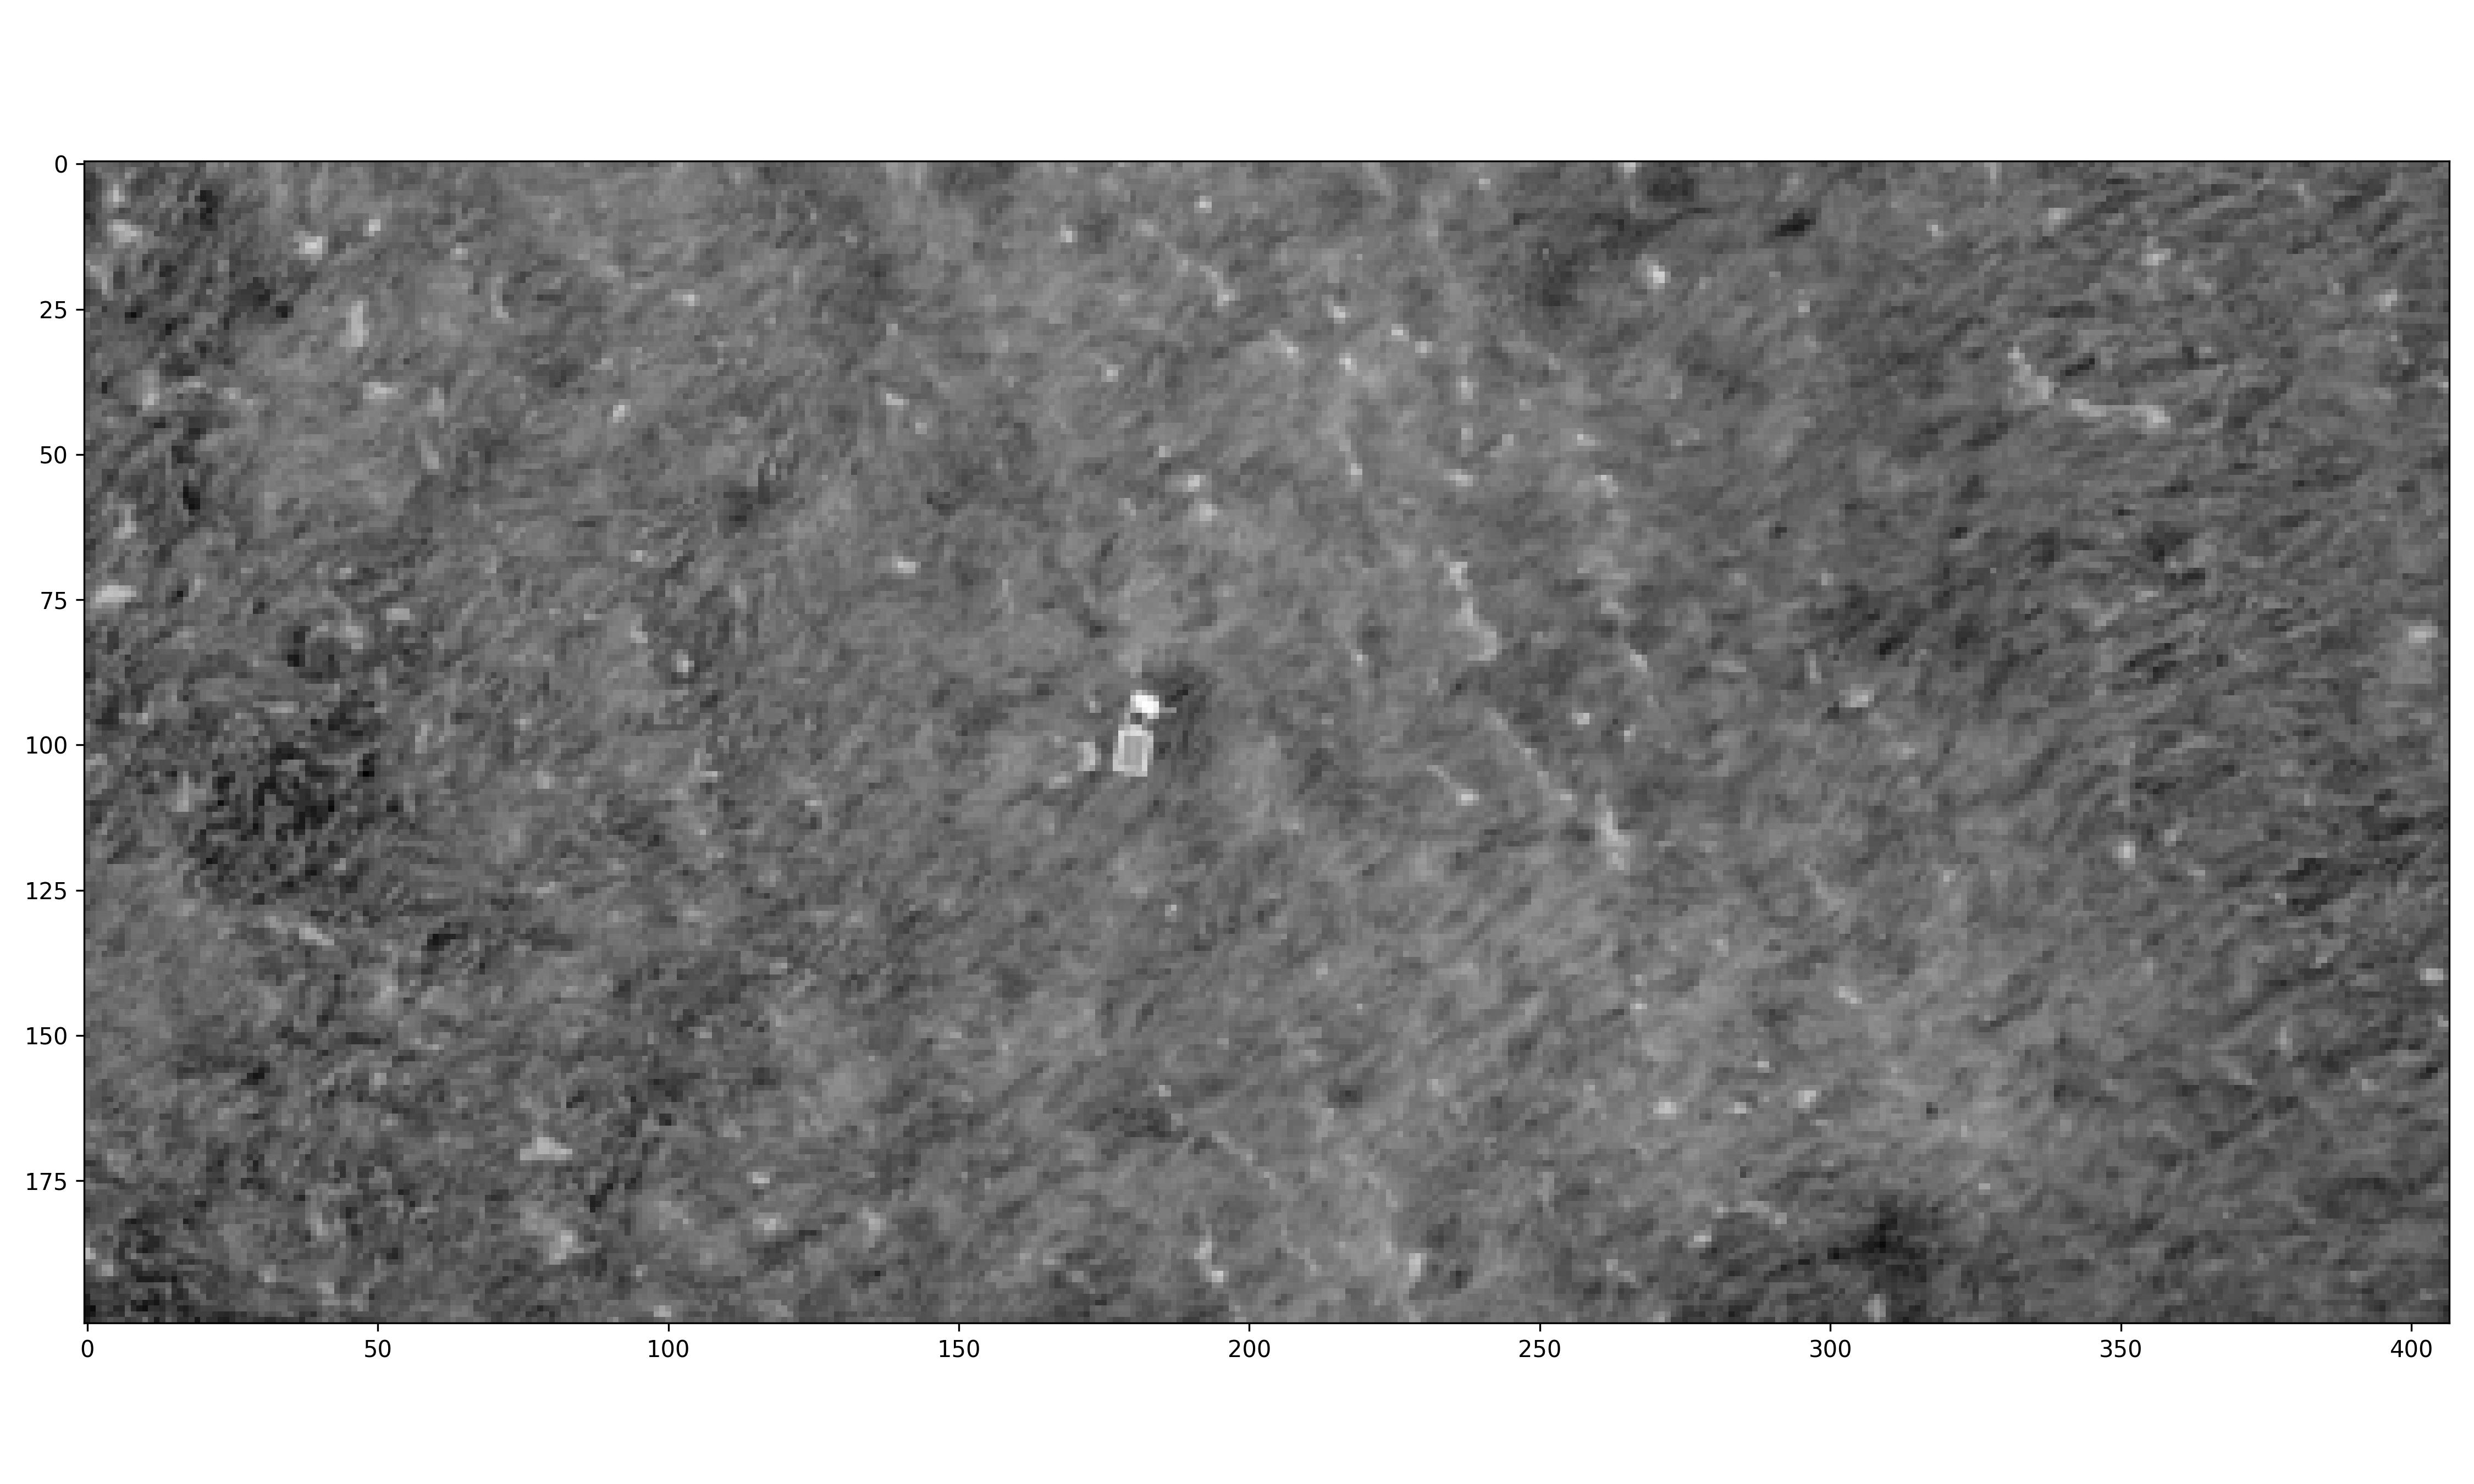
\includegraphics{images/plots/grass/1.jpg}

}

\subcaption{Living Labs Aerial Image}

\end{figure}%

\end{minipage}%
%
\begin{minipage}{0.33\linewidth}

\begin{figure}[H]

{\centering 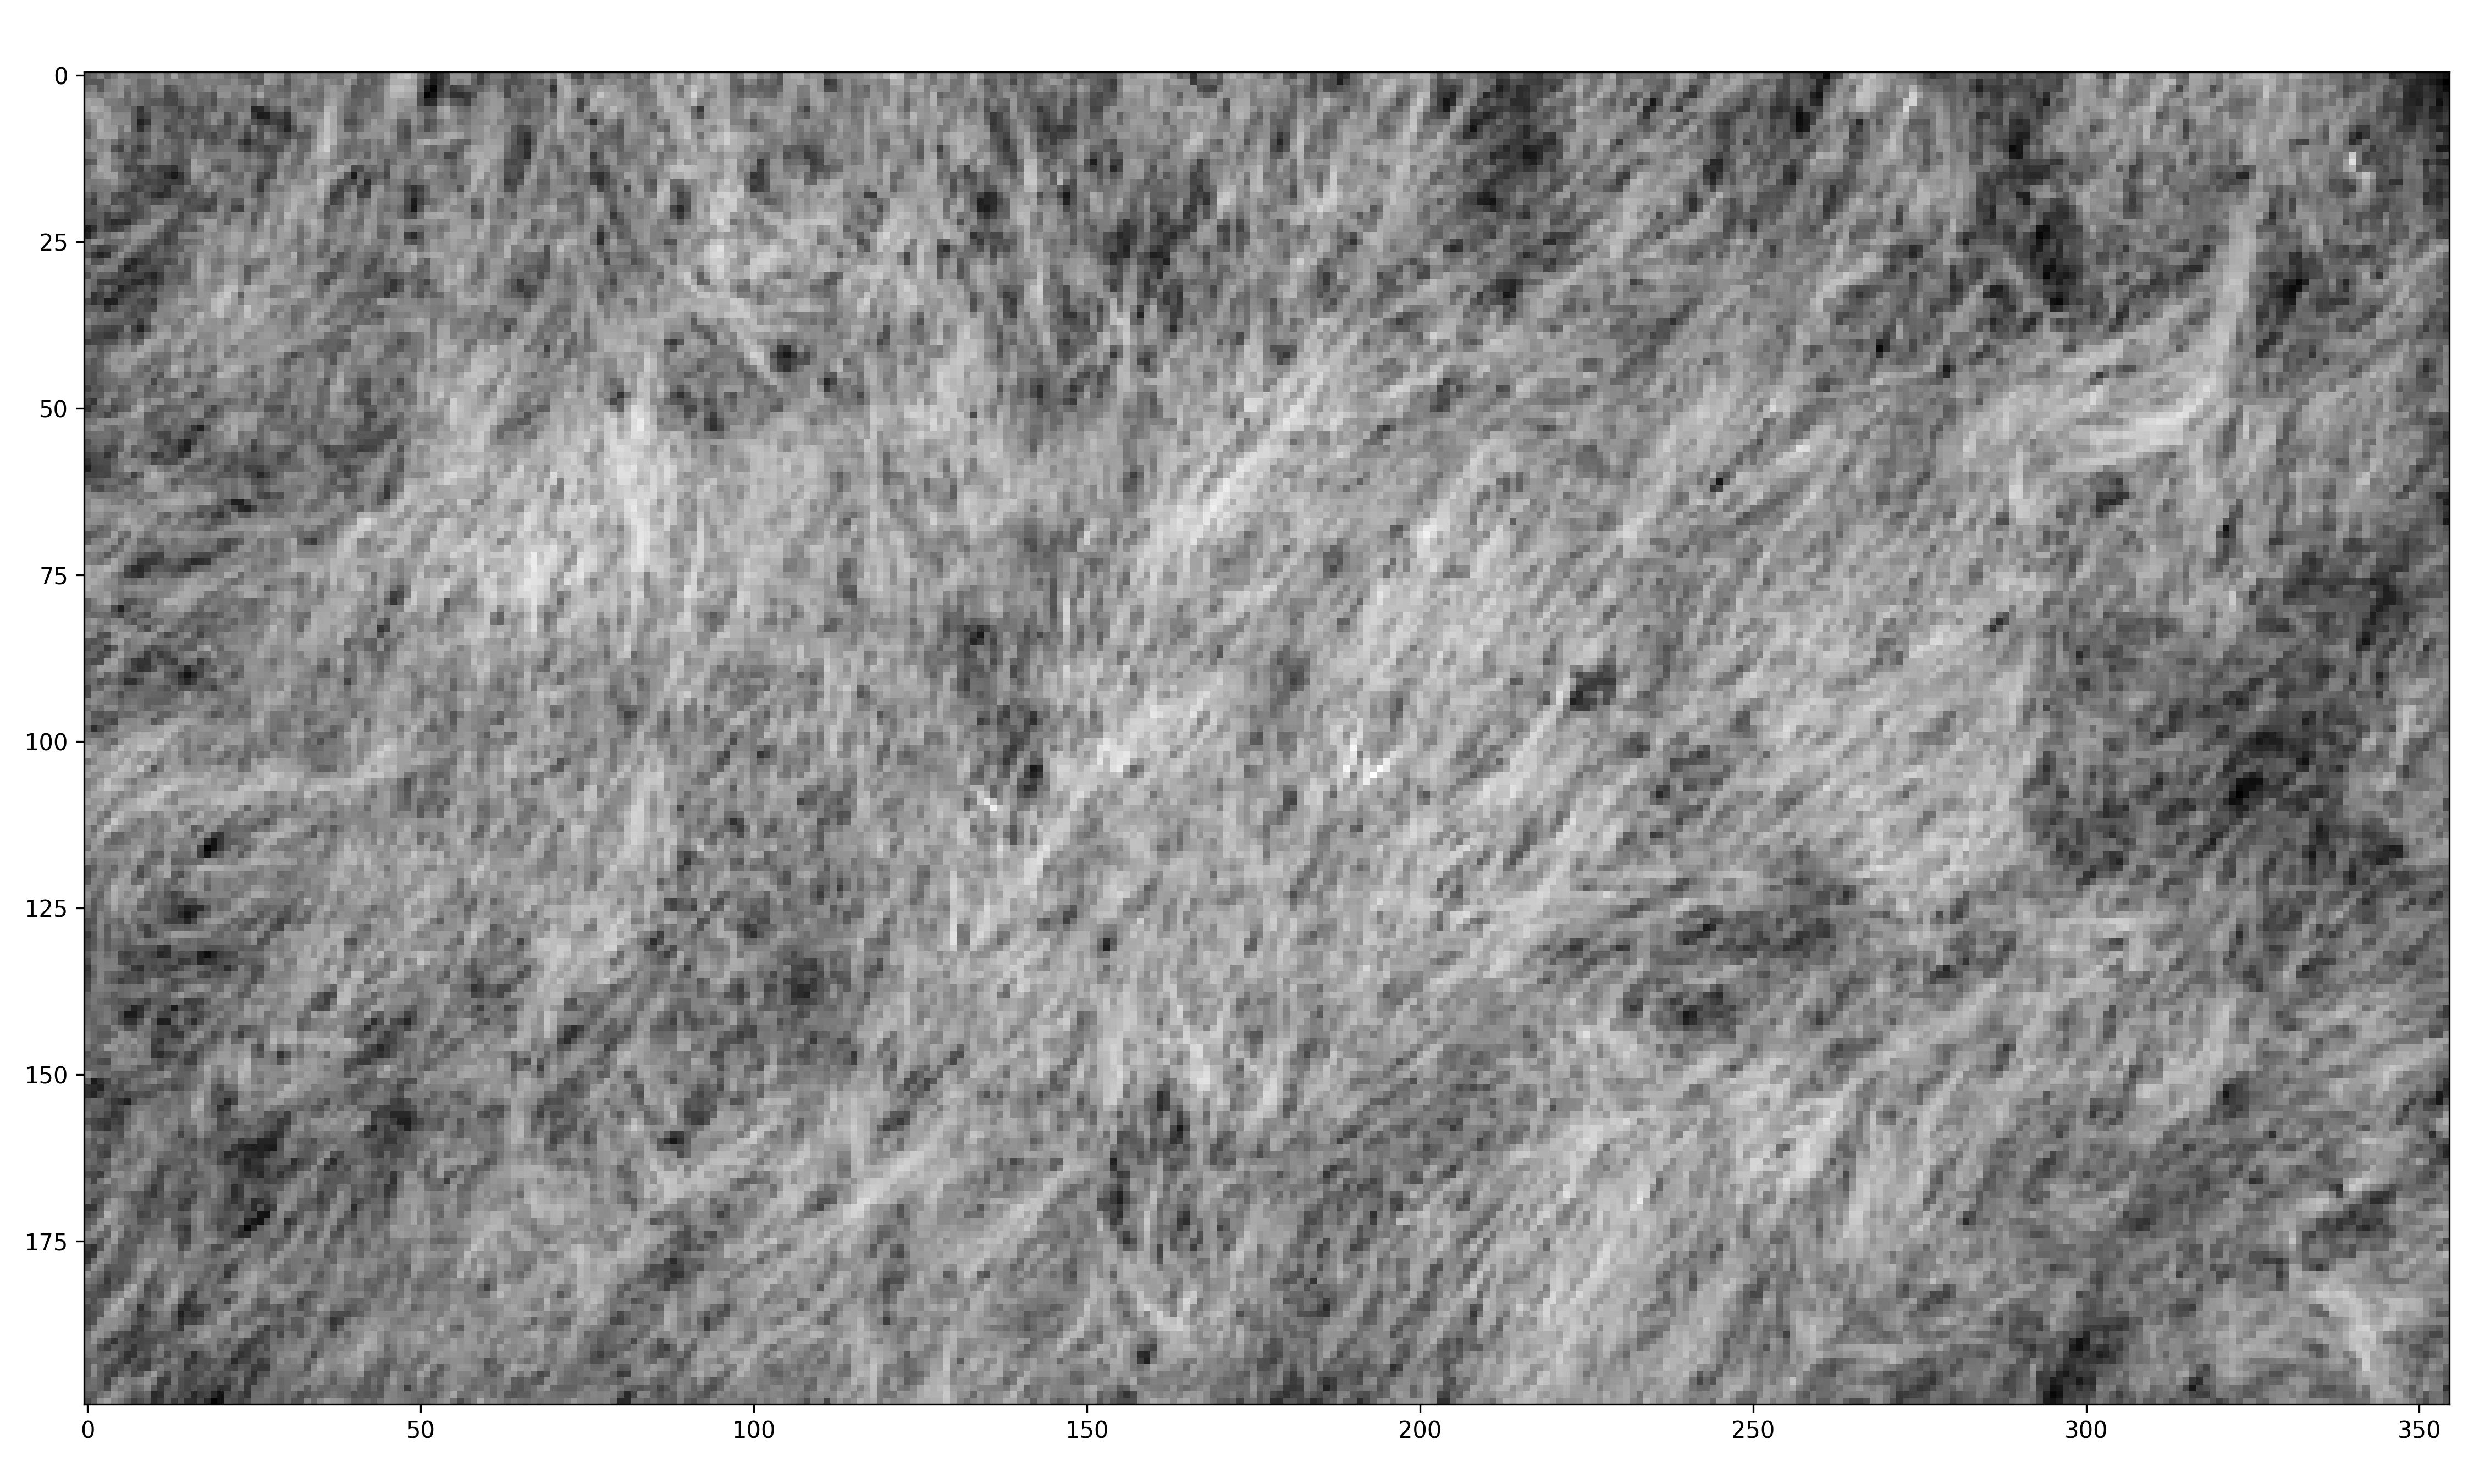
\includegraphics{images/plots/grass/2.jpg}

}

\subcaption{Living Labs Close-Up Image}

\end{figure}%

\end{minipage}%

\caption{\label{fig-grass-images}Grass Images Rescaled and Converted to
Greyscale}

\end{figure}%

\section{Build Data Frames for Each Grass
Image}\label{build-data-frames-for-each-grass-image}

\begin{Shaded}
\begin{Highlighting}[]
\CommentTok{\# Internet grass DF of gradient magnitudes and angles}
\NormalTok{mag\_internet\_grass }\OperatorTok{=}\NormalTok{ np.array(mag\_list[}\DecValTok{0}\NormalTok{])}
\NormalTok{theta\_internet\_grass }\OperatorTok{=}\NormalTok{ np.array(theta\_list[}\DecValTok{0}\NormalTok{])}

\CommentTok{\# Aerial Living Labs DF of gradient magnitudes and angles}
\NormalTok{mag\_aerial\_living\_lab }\OperatorTok{=}\NormalTok{ np.array(mag\_list[}\DecValTok{1}\NormalTok{])}
\NormalTok{theta\_aerial\_living\_lab }\OperatorTok{=}\NormalTok{ np.array(theta\_list[}\DecValTok{1}\NormalTok{])}

\CommentTok{\# Close{-}up Living Labs DF of gradient magnitudes and angles}
\NormalTok{mag\_close\_up\_living\_lab }\OperatorTok{=}\NormalTok{ np.array(mag\_list[}\DecValTok{2}\NormalTok{])}
\NormalTok{theta\_close\_up\_living\_lab }\OperatorTok{=}\NormalTok{ np.array(theta\_list[}\DecValTok{2}\NormalTok{])}
\end{Highlighting}
\end{Shaded}

\section{Extract Gradient Magnitudes and Angles from each Grass
Image}\label{extract-gradient-magnitudes-and-angles-from-each-grass-image}

\begin{Shaded}
\begin{Highlighting}[]
\CommentTok{\# Save gradient magnitudes of Internet Grass in image form}

\CommentTok{\# plt.figure(figsize=(15, 8))}
\CommentTok{\# \#plt.title(\textquotesingle{}San Francisco, CA Gradient Magnitudes\textquotesingle{})}
\CommentTok{\# plt.imshow(mag\_list[0], cmap="gray")}
\CommentTok{\# plt.axis("on")}
\CommentTok{\# \#plt.show()}
\CommentTok{\# plt.tight\_layout()}
\CommentTok{\# plt.savefig("images/plots/grass/internet\_grass\_mag.png", dpi=300)}
\end{Highlighting}
\end{Shaded}

\begin{Shaded}
\begin{Highlighting}[]
\CommentTok{\# Save gradient magnitudes of Aerial Living Labs in image form}

\CommentTok{\# plt.figure(figsize=(15, 8))}
\CommentTok{\# \#plt.title(\textquotesingle{}Salt Lake City, UT Gradient Magnitudes\textquotesingle{})}
\CommentTok{\# plt.imshow(mag\_list[1], cmap="gray")}
\CommentTok{\# plt.axis("on")}
\CommentTok{\# \#plt.show()}
\CommentTok{\# plt.tight\_layout()}
\CommentTok{\# plt.savefig("images/plots/grass/aerial\_living\_lab\_grass\_mag.png", dpi=300)}
\end{Highlighting}
\end{Shaded}

\begin{Shaded}
\begin{Highlighting}[]
\CommentTok{\# Save gradient magnitudes of Close{-}Up Living Labs in image form}

\CommentTok{\# plt.figure(figsize=(15, 8))}
\CommentTok{\# \#plt.title(\textquotesingle{}Detroit, MI Gradient Magnitudes\textquotesingle{})}
\CommentTok{\# plt.imshow(mag\_list[2], cmap="gray")}
\CommentTok{\# plt.axis("on")}
\CommentTok{\# \#plt.show()}
\CommentTok{\# plt.tight\_layout()}
\CommentTok{\# plt.savefig("images/plots/grass/close\_up\_living\_lab\_grass\_mag.png", dpi=300)}
\end{Highlighting}
\end{Shaded}

\begin{figure}

\begin{minipage}{0.33\linewidth}

\begin{figure}[H]

{\centering 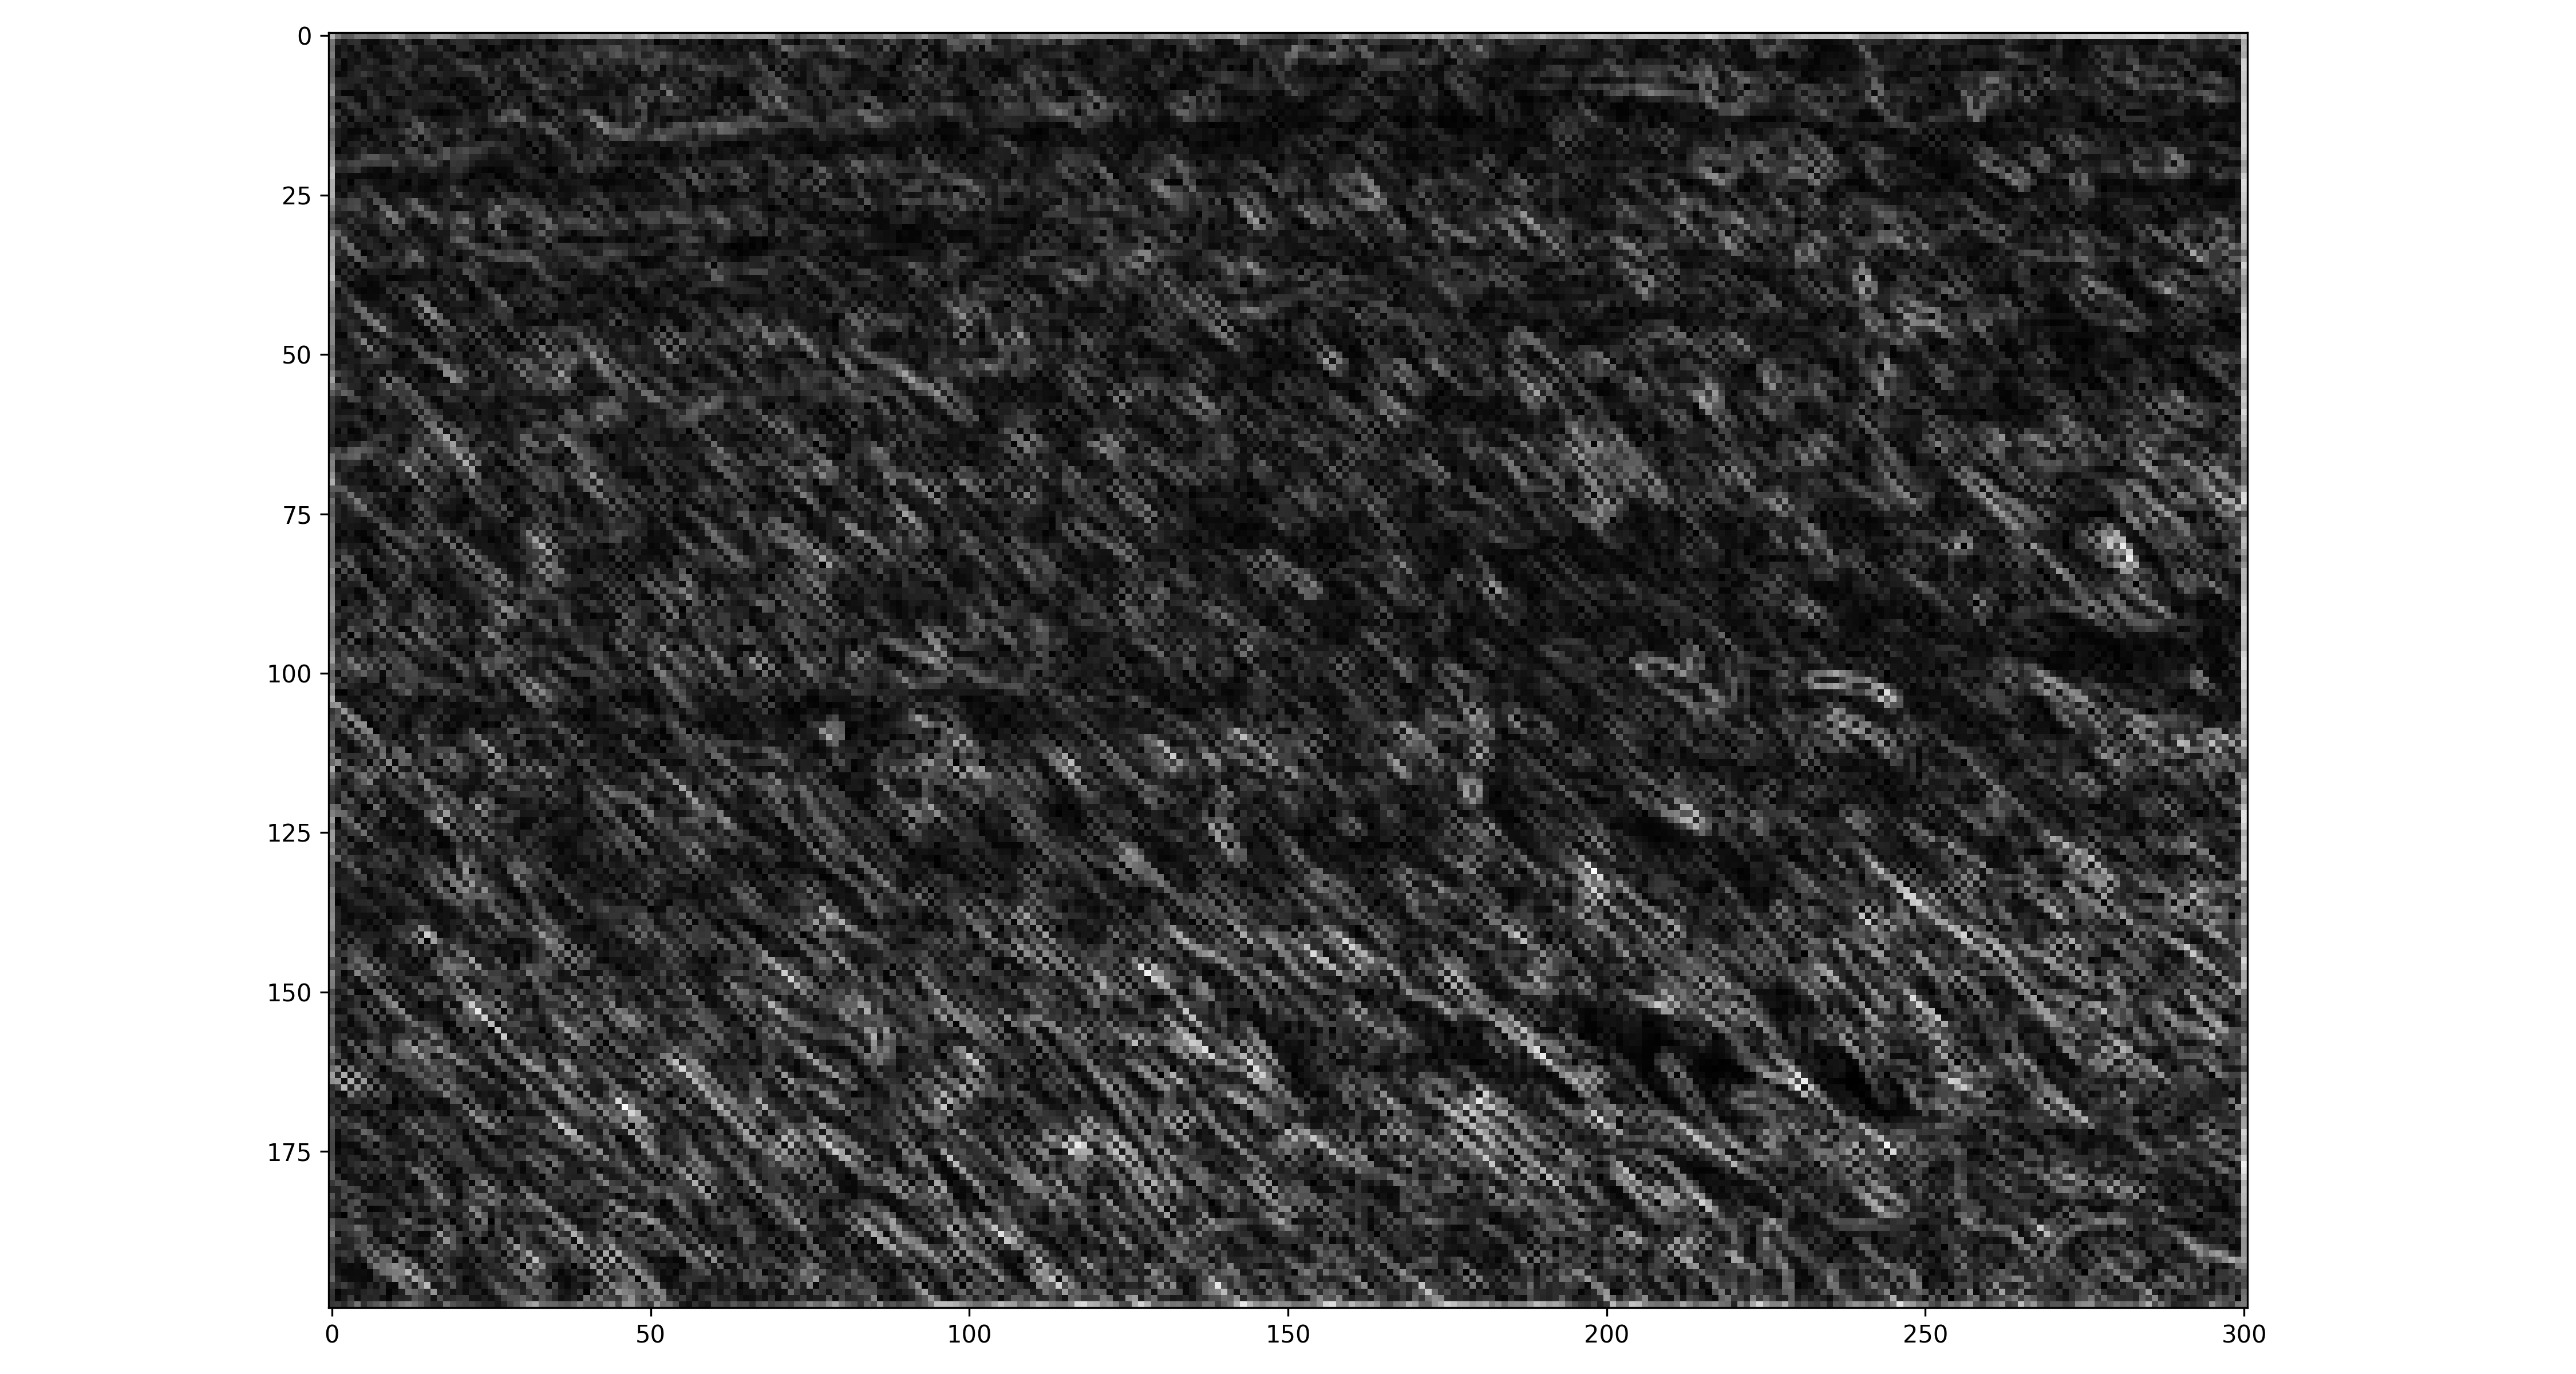
\includegraphics{images/plots/grass/internet_grass_mag.png}

}

\subcaption{Internet Grass}

\end{figure}%

\end{minipage}%
%
\begin{minipage}{0.33\linewidth}

\begin{figure}[H]

{\centering 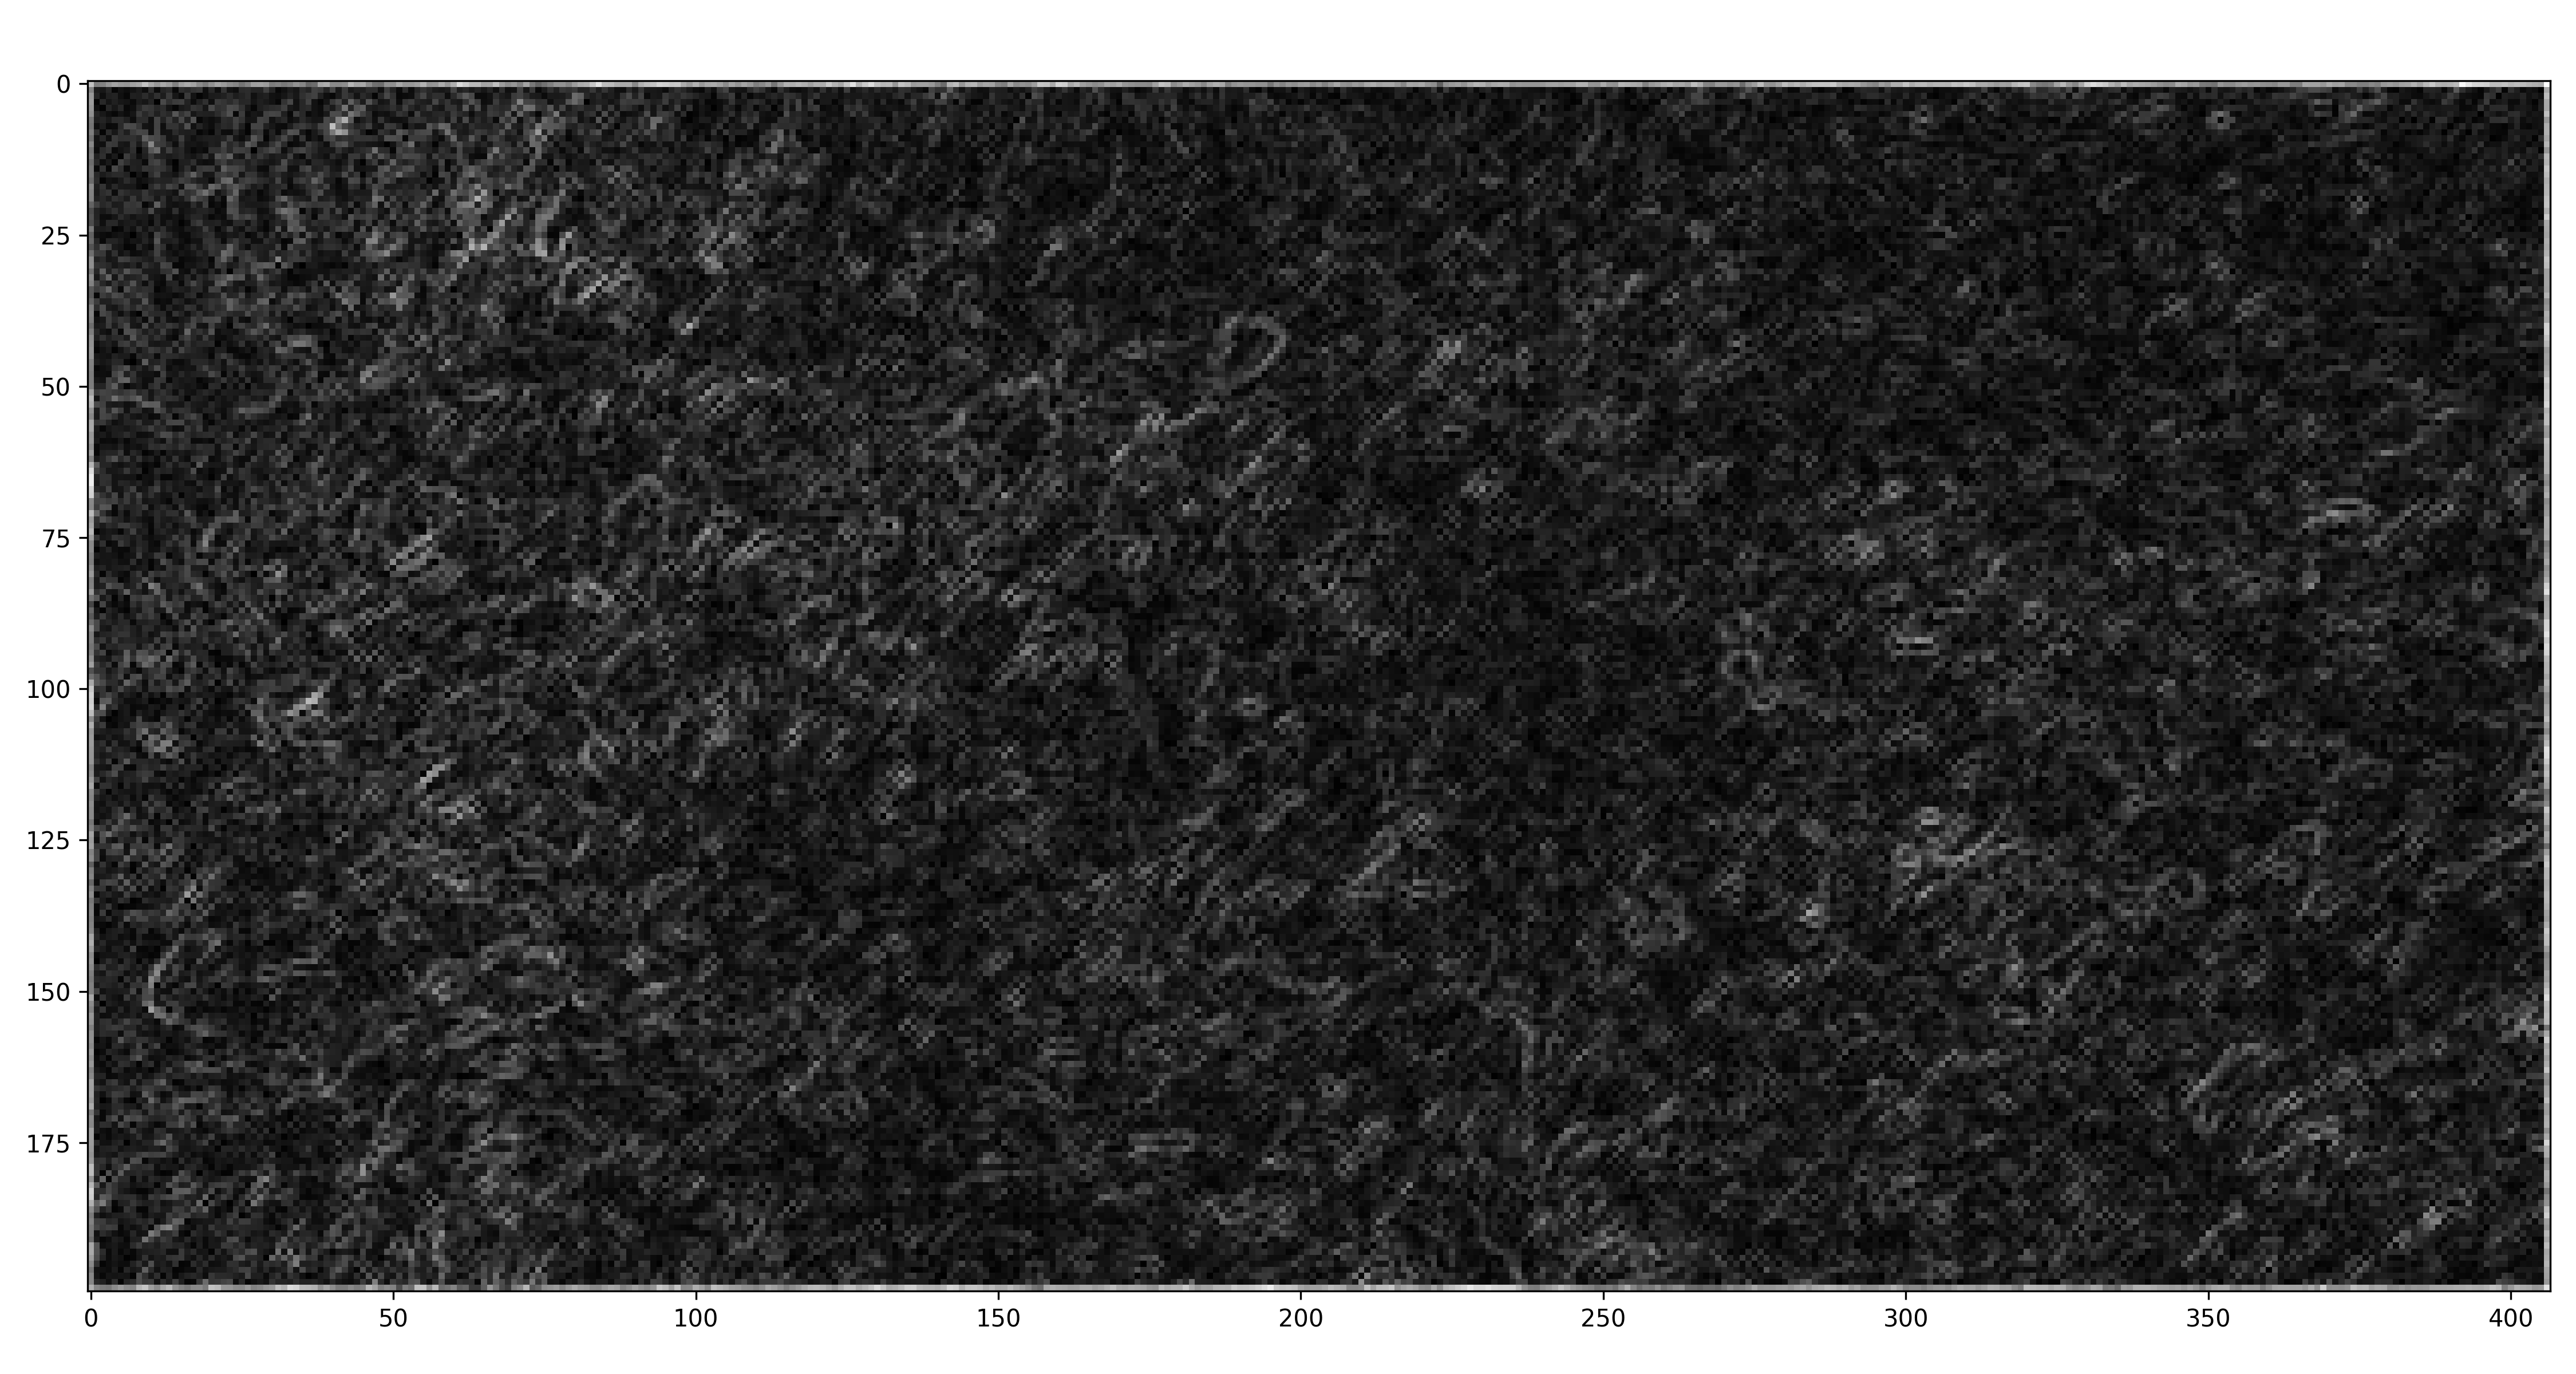
\includegraphics{images/plots/grass/aerial_living_lab_grass_mag.png}

}

\subcaption{Aerial Living Labs}

\end{figure}%

\end{minipage}%
%
\begin{minipage}{0.33\linewidth}

\begin{figure}[H]

{\centering 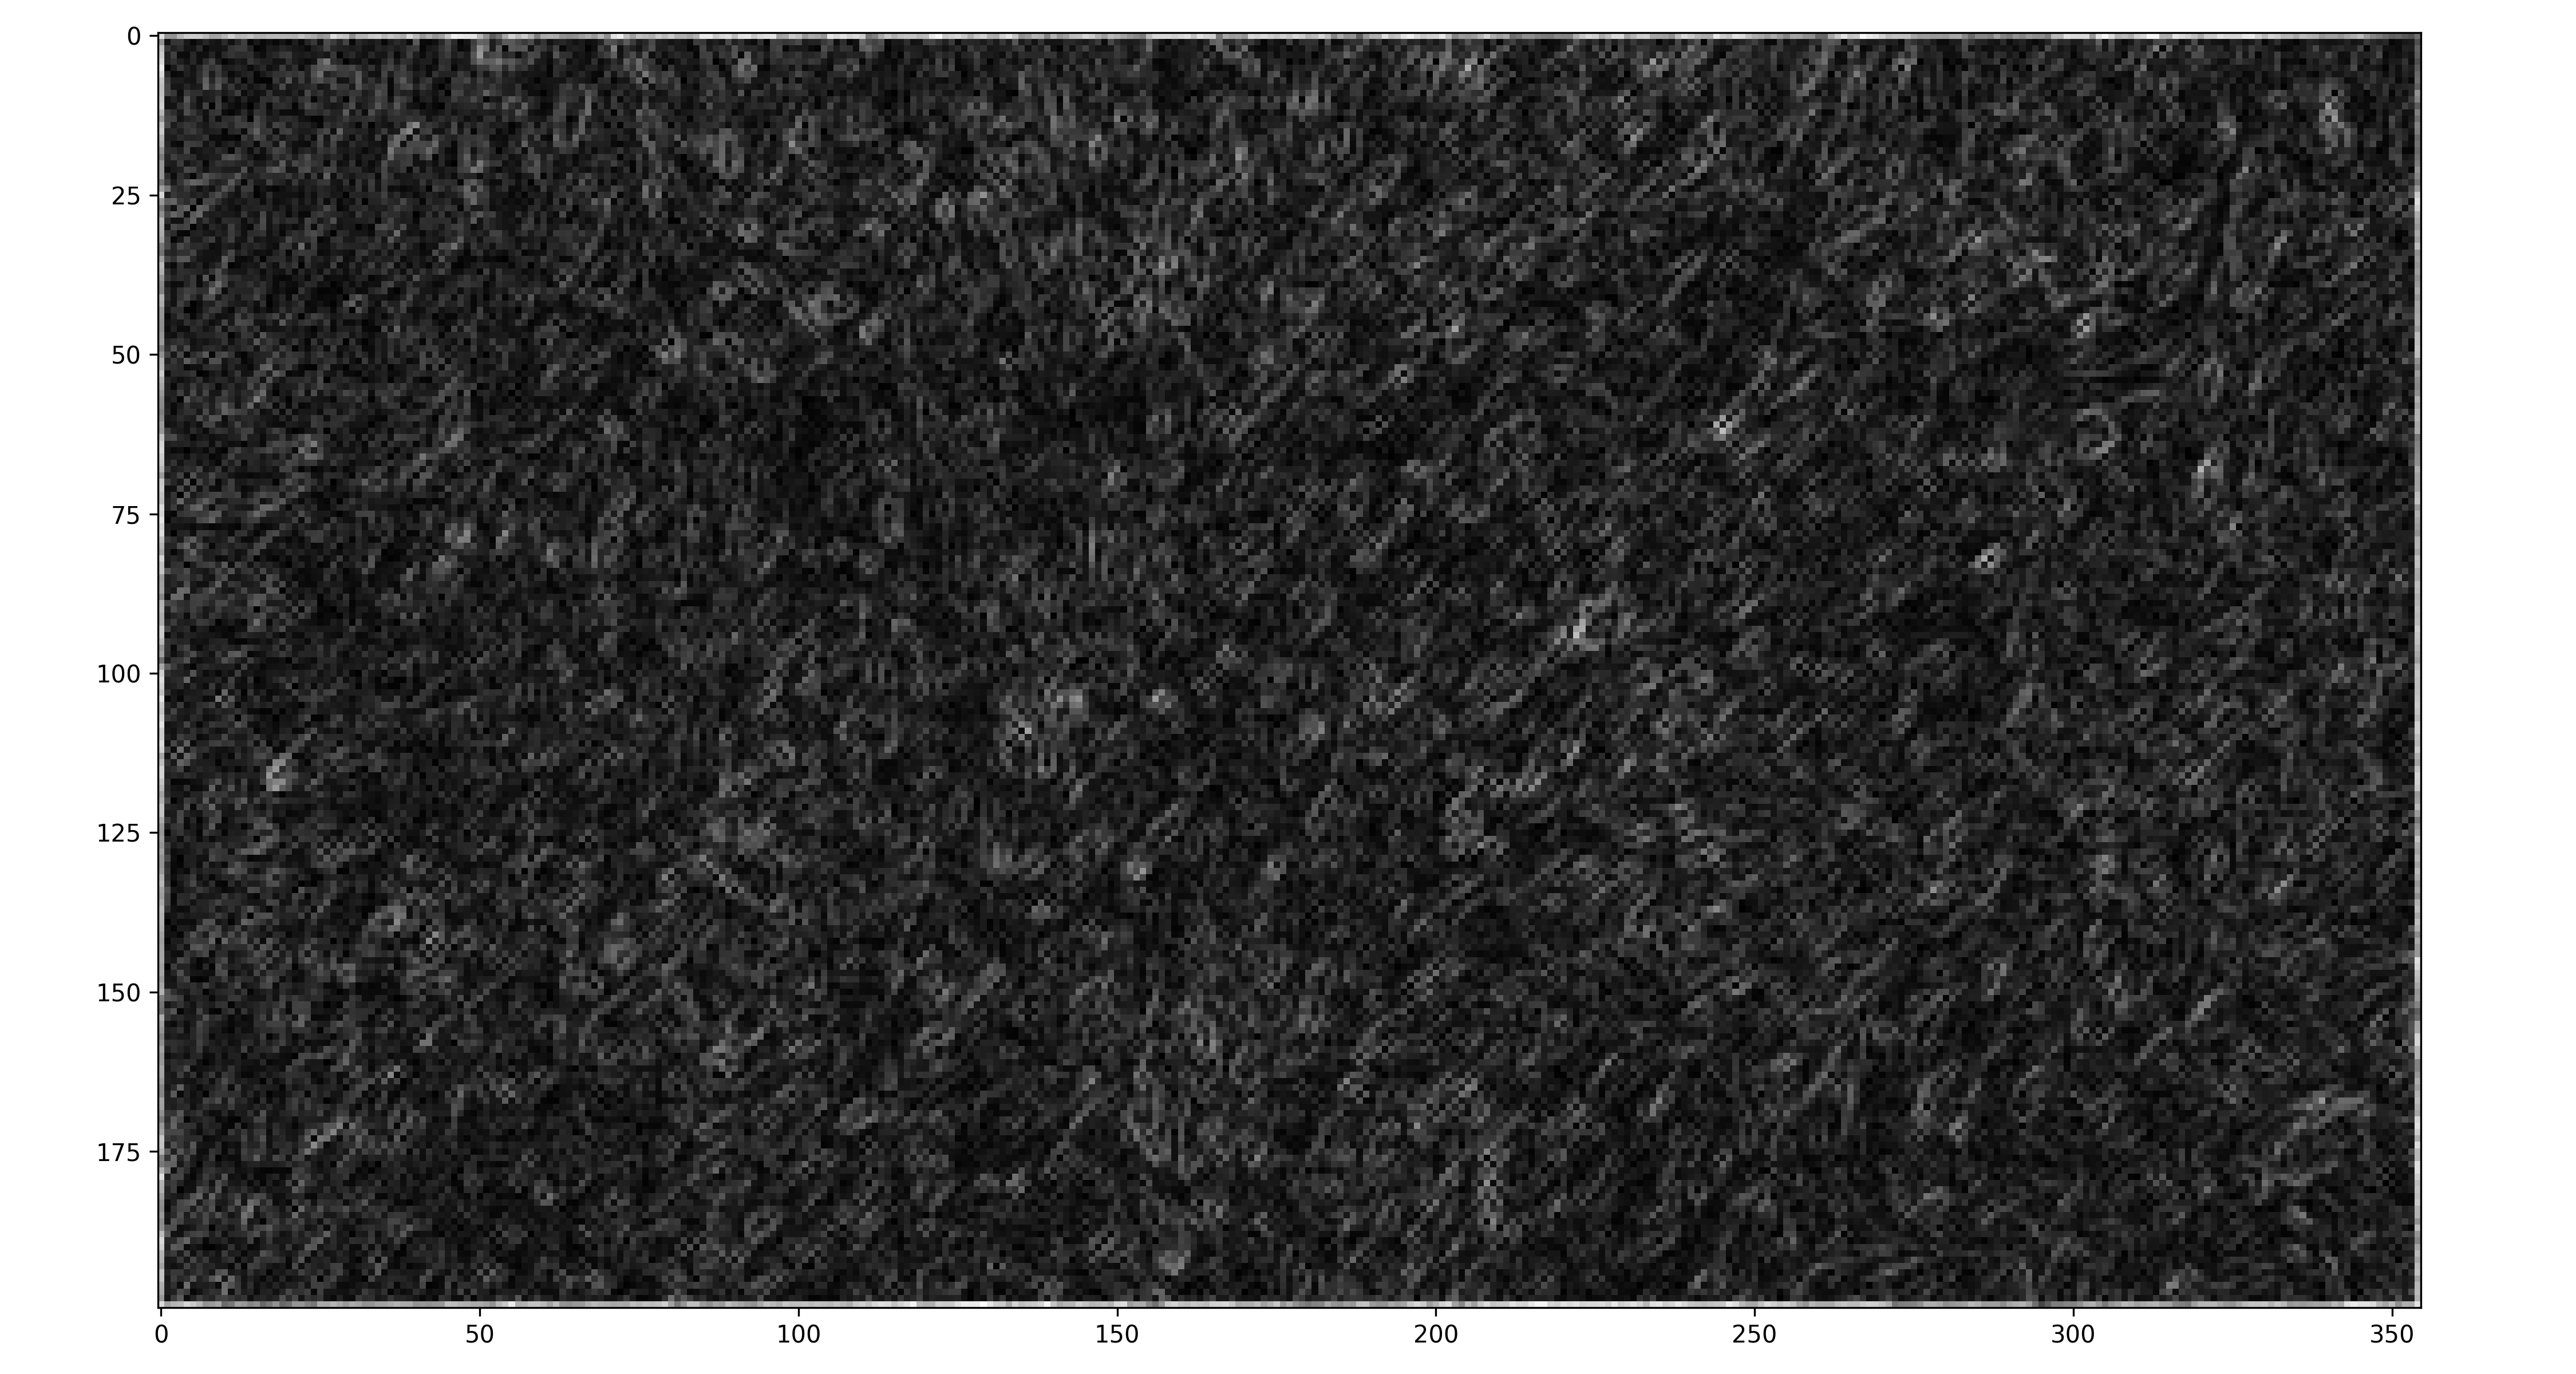
\includegraphics{images/plots/grass/close_up_living_lab_grass_mag.png}

}

\subcaption{Close-Up Living Labs}

\end{figure}%

\end{minipage}%

\caption{\label{fig-grass-mags}Grass Image Magnitudes}

\end{figure}%

\section{Create Data Frame for Each
Image}\label{create-data-frame-for-each-image-1}

\begin{Shaded}
\begin{Highlighting}[]
\CommentTok{\# Internet grass DF}
\NormalTok{internet\_grass\_hog\_df }\OtherTok{\textless{}{-}} \FunctionTok{data.frame}\NormalTok{(}\AttributeTok{mag =} \FunctionTok{as.vector}\NormalTok{(py}\SpecialCharTok{$}\NormalTok{mag\_internet\_grass),}
                              \AttributeTok{theta =} \FunctionTok{as.vector}\NormalTok{((py}\SpecialCharTok{$}\NormalTok{theta\_internet\_grass))) }\SpecialCharTok{\%\textgreater{}\%}
  \FunctionTok{mutate}\NormalTok{(}\AttributeTok{radian =}\NormalTok{ theta}\SpecialCharTok{*}\NormalTok{(pi}\SpecialCharTok{/}\DecValTok{180}\NormalTok{))}
\end{Highlighting}
\end{Shaded}

\begin{Shaded}
\begin{Highlighting}[]
\CommentTok{\# Aerial Living Labs DF}
\NormalTok{aerial\_living\_lab\_hog\_df }\OtherTok{\textless{}{-}} \FunctionTok{data.frame}\NormalTok{(}\AttributeTok{mag =} \FunctionTok{as.vector}\NormalTok{(py}\SpecialCharTok{$}\NormalTok{mag\_aerial\_living\_lab),}
                              \AttributeTok{theta =} \FunctionTok{as.vector}\NormalTok{((py}\SpecialCharTok{$}\NormalTok{theta\_aerial\_living\_lab))) }\SpecialCharTok{\%\textgreater{}\%}
  \FunctionTok{mutate}\NormalTok{(}\AttributeTok{radian =}\NormalTok{ theta}\SpecialCharTok{*}\NormalTok{(pi}\SpecialCharTok{/}\DecValTok{180}\NormalTok{))}
\end{Highlighting}
\end{Shaded}

\begin{Shaded}
\begin{Highlighting}[]
\CommentTok{\# Close{-}up Living Labs DF}
\NormalTok{close\_up\_living\_lab\_hog\_df }\OtherTok{\textless{}{-}} \FunctionTok{data.frame}\NormalTok{(}\AttributeTok{mag =} \FunctionTok{as.vector}\NormalTok{(py}\SpecialCharTok{$}\NormalTok{mag\_close\_up\_living\_lab),}
                              \AttributeTok{theta =} \FunctionTok{as.vector}\NormalTok{((py}\SpecialCharTok{$}\NormalTok{theta\_close\_up\_living\_lab))) }\SpecialCharTok{\%\textgreater{}\%}
  \FunctionTok{mutate}\NormalTok{(}\AttributeTok{radian =}\NormalTok{ theta}\SpecialCharTok{*}\NormalTok{(pi}\SpecialCharTok{/}\DecValTok{180}\NormalTok{))}
\end{Highlighting}
\end{Shaded}

\begin{Shaded}
\begin{Highlighting}[]
\CommentTok{\# List of all Data frames}
\NormalTok{grass\_standard\_df\_list }\OtherTok{=} \FunctionTok{list}\NormalTok{(internet\_grass\_hog\_df,}
\NormalTok{                        aerial\_living\_lab\_hog\_df, }
\NormalTok{                        close\_up\_living\_lab\_hog\_df)}
\end{Highlighting}
\end{Shaded}

\section{Create Histograms of Gradient Magnitudes and Angles for Grass
Images}\label{create-histograms-of-gradient-magnitudes-and-angles-for-grass-images}

\begin{Shaded}
\begin{Highlighting}[]
\CommentTok{\# Internet grass image histogram of gradient mags}
\NormalTok{internet\_grass\_histogram\_mag\_plot }\OtherTok{\textless{}{-}}
  \FunctionTok{ggplot}\NormalTok{(grass\_standard\_df\_list[[}\DecValTok{1}\NormalTok{]], }
         \FunctionTok{aes}\NormalTok{(}\AttributeTok{x =}\NormalTok{ mag)) }\SpecialCharTok{+}
  \FunctionTok{geom\_histogram}\NormalTok{(}\AttributeTok{colour =} \StringTok{"black"}\NormalTok{, }\AttributeTok{fill =} \StringTok{"lightblue"}\NormalTok{) }\SpecialCharTok{+}
  \FunctionTok{scale\_x\_continuous}\NormalTok{() }\SpecialCharTok{+} 
  \FunctionTok{labs}\NormalTok{(}\AttributeTok{x =} \StringTok{"Gradient Magnitude"}\NormalTok{, }
       \AttributeTok{y =} \StringTok{"Count"}\NormalTok{, }
       \AttributeTok{title =} \StringTok{"Internet Grass Image Histogram of Gradient Magnitudes"}
\NormalTok{       ) }\SpecialCharTok{+}
  \FunctionTok{theme\_minimal}\NormalTok{() }\SpecialCharTok{+}
  \FunctionTok{theme}\NormalTok{(}\AttributeTok{plot.title =} \FunctionTok{element\_text}\NormalTok{(}\AttributeTok{hjust =} \FloatTok{0.5}\NormalTok{))}

\CommentTok{\# Internet grass mag filter}
\NormalTok{internet\_grass\_mag\_filter }\OtherTok{\textless{}{-}} \FloatTok{0.3}

\CommentTok{\# save image}
\FunctionTok{ggsave}\NormalTok{(}\StringTok{"images/plots/grass/internet\_grass\_histogram\_mag\_plot.jpg"}\NormalTok{, internet\_grass\_histogram\_mag\_plot, }\AttributeTok{width =} \DecValTok{6}\NormalTok{, }\AttributeTok{height =} \DecValTok{4}\NormalTok{, }\AttributeTok{dpi =} \DecValTok{300}\NormalTok{)}
\end{Highlighting}
\end{Shaded}

\begin{Shaded}
\begin{Highlighting}[]
\CommentTok{\# Internet grass image histogram of gradient angles}
\NormalTok{internet\_grass\_histogram\_theta\_plot }\OtherTok{\textless{}{-}}
  \FunctionTok{ggplot}\NormalTok{(grass\_standard\_df\_list[[}\DecValTok{1}\NormalTok{]], }
         \FunctionTok{aes}\NormalTok{(}\AttributeTok{x =}\NormalTok{ theta)) }\SpecialCharTok{+}
  \FunctionTok{geom\_histogram}\NormalTok{(}\AttributeTok{colour =} \StringTok{"black"}\NormalTok{, }\AttributeTok{fill =} \StringTok{"lightblue"}\NormalTok{) }\SpecialCharTok{+}
  \FunctionTok{scale\_x\_continuous}\NormalTok{() }\SpecialCharTok{+} 
  \FunctionTok{labs}\NormalTok{(}\AttributeTok{x =} \StringTok{"Gradient Angle"}\NormalTok{, }
       \AttributeTok{y =} \StringTok{"Count"}\NormalTok{, }
       \AttributeTok{title =} \StringTok{"Internet Grass Image Histogram of Gradient Angles"}
\NormalTok{       ) }\SpecialCharTok{+}
  \FunctionTok{theme\_minimal}\NormalTok{() }\SpecialCharTok{+}
  \FunctionTok{theme}\NormalTok{(}\AttributeTok{plot.title =} \FunctionTok{element\_text}\NormalTok{(}\AttributeTok{hjust =} \FloatTok{0.5}\NormalTok{))}

\CommentTok{\# save image}
\FunctionTok{ggsave}\NormalTok{(}\StringTok{"images/plots/grass/internet\_grass\_histogram\_theta\_plot.jpg"}\NormalTok{, internet\_grass\_histogram\_theta\_plot, }\AttributeTok{width =} \DecValTok{6}\NormalTok{, }\AttributeTok{height =} \DecValTok{4}\NormalTok{, }\AttributeTok{dpi =} \DecValTok{300}\NormalTok{)}
\end{Highlighting}
\end{Shaded}

\begin{Shaded}
\begin{Highlighting}[]
\CommentTok{\# Aerial Living Labs image histogram of gradient mags}
\NormalTok{aerial\_living\_lab\_histogram\_mag\_plot }\OtherTok{\textless{}{-}}
  \FunctionTok{ggplot}\NormalTok{(grass\_standard\_df\_list[[}\DecValTok{2}\NormalTok{]], }
         \FunctionTok{aes}\NormalTok{(}\AttributeTok{x =}\NormalTok{ mag)) }\SpecialCharTok{+}
  \FunctionTok{geom\_histogram}\NormalTok{(}\AttributeTok{colour =} \StringTok{"black"}\NormalTok{, }\AttributeTok{fill =} \StringTok{"lightblue"}\NormalTok{) }\SpecialCharTok{+}
  \FunctionTok{scale\_x\_continuous}\NormalTok{() }\SpecialCharTok{+} 
  \FunctionTok{labs}\NormalTok{(}\AttributeTok{x =} \StringTok{"Gradient Magnitude"}\NormalTok{, }
       \AttributeTok{y =} \StringTok{"Count"}\NormalTok{, }
       \AttributeTok{title =} \StringTok{"Aerial Living Labs Image Histogram of Gradient Magnitudes"}
\NormalTok{  ) }\SpecialCharTok{+}
  \FunctionTok{theme\_minimal}\NormalTok{() }\SpecialCharTok{+}
  \FunctionTok{theme}\NormalTok{(}\AttributeTok{plot.title =} \FunctionTok{element\_text}\NormalTok{(}\AttributeTok{hjust =} \FloatTok{0.5}\NormalTok{))}

\CommentTok{\# Aerial Living Labs mag filter}
\NormalTok{aerial\_living\_lab\_mag\_filter }\OtherTok{\textless{}{-}} \FloatTok{0.08}

\CommentTok{\# save image}
\FunctionTok{ggsave}\NormalTok{(}\StringTok{"images/plots/grass/aerial\_living\_lab\_histogram\_mag\_plot.jpg"}\NormalTok{, }
\NormalTok{       aerial\_living\_lab\_histogram\_mag\_plot, }\AttributeTok{width =} \DecValTok{6}\NormalTok{, }\AttributeTok{height =} \DecValTok{4}\NormalTok{, }\AttributeTok{dpi =} \DecValTok{300}\NormalTok{)}
\end{Highlighting}
\end{Shaded}

\begin{Shaded}
\begin{Highlighting}[]
\CommentTok{\# Aerial Living Labs image histogram of gradient angles}
\NormalTok{aerial\_living\_lab\_histogram\_theta\_plot }\OtherTok{\textless{}{-}}
  \FunctionTok{ggplot}\NormalTok{(grass\_standard\_df\_list[[}\DecValTok{2}\NormalTok{]], }
         \FunctionTok{aes}\NormalTok{(}\AttributeTok{x =}\NormalTok{ theta)) }\SpecialCharTok{+}
  \FunctionTok{geom\_histogram}\NormalTok{(}\AttributeTok{colour =} \StringTok{"black"}\NormalTok{, }\AttributeTok{fill =} \StringTok{"lightblue"}\NormalTok{) }\SpecialCharTok{+}
  \FunctionTok{scale\_x\_continuous}\NormalTok{() }\SpecialCharTok{+} 
  \FunctionTok{labs}\NormalTok{(}\AttributeTok{x =} \StringTok{"Gradient Angle"}\NormalTok{, }
       \AttributeTok{y =} \StringTok{"Count"}\NormalTok{, }
       \AttributeTok{title =} \StringTok{"Aerial Living Labs Image Histogram of Gradient Angles"}
\NormalTok{  ) }\SpecialCharTok{+}
  \FunctionTok{theme\_minimal}\NormalTok{() }\SpecialCharTok{+}
  \FunctionTok{theme}\NormalTok{(}\AttributeTok{plot.title =} \FunctionTok{element\_text}\NormalTok{(}\AttributeTok{hjust =} \FloatTok{0.5}\NormalTok{))}

\CommentTok{\# save image}
\FunctionTok{ggsave}\NormalTok{(}\StringTok{"images/plots/grass/aerial\_living\_lab\_histogram\_theta\_plot.jpg"}\NormalTok{, }
\NormalTok{       aerial\_living\_lab\_histogram\_theta\_plot, }\AttributeTok{width =} \DecValTok{6}\NormalTok{, }\AttributeTok{height =} \DecValTok{4}\NormalTok{, }\AttributeTok{dpi =} \DecValTok{300}\NormalTok{)}
\end{Highlighting}
\end{Shaded}

\begin{Shaded}
\begin{Highlighting}[]
\CommentTok{\# Close{-}up Living Labs image histogram of gradient mags}
\NormalTok{close\_up\_living\_lab\_histogram\_mag\_plot }\OtherTok{\textless{}{-}}
  \FunctionTok{ggplot}\NormalTok{(grass\_standard\_df\_list[[}\DecValTok{3}\NormalTok{]], }
         \FunctionTok{aes}\NormalTok{(}\AttributeTok{x =}\NormalTok{ mag)) }\SpecialCharTok{+}
  \FunctionTok{geom\_histogram}\NormalTok{(}\AttributeTok{colour =} \StringTok{"black"}\NormalTok{, }\AttributeTok{fill =} \StringTok{"lightblue"}\NormalTok{) }\SpecialCharTok{+}
  \FunctionTok{scale\_x\_continuous}\NormalTok{() }\SpecialCharTok{+} 
  \FunctionTok{labs}\NormalTok{(}\AttributeTok{x =} \StringTok{"Gradient Magnitude"}\NormalTok{, }
       \AttributeTok{y =} \StringTok{"Count"}\NormalTok{, }
       \AttributeTok{title =} \StringTok{"Close{-}Up Living Labs Histogram of Gradient Magnitudes"}
\NormalTok{       ) }\SpecialCharTok{+}
  \FunctionTok{theme\_minimal}\NormalTok{() }\SpecialCharTok{+}
  \FunctionTok{theme}\NormalTok{(}\AttributeTok{plot.title =} \FunctionTok{element\_text}\NormalTok{(}\AttributeTok{hjust =} \FloatTok{0.5}\NormalTok{))}

\CommentTok{\# Close{-}up mag filter}
\NormalTok{close\_up\_living\_lab\_mag\_filter }\OtherTok{\textless{}{-}} \FloatTok{0.12}

\CommentTok{\# save image}
\FunctionTok{ggsave}\NormalTok{(}\StringTok{"images/plots/grass/close\_up\_living\_lab\_histogram\_mag\_plot.jpg"}\NormalTok{, close\_up\_living\_lab\_histogram\_mag\_plot, }\AttributeTok{width =} \DecValTok{6}\NormalTok{, }\AttributeTok{height =} \DecValTok{4}\NormalTok{, }\AttributeTok{dpi =} \DecValTok{300}\NormalTok{)}
\end{Highlighting}
\end{Shaded}

\begin{Shaded}
\begin{Highlighting}[]
\CommentTok{\# Close{-}up Living Labs image histogram of gradient angles}
\NormalTok{close\_up\_living\_lab\_histogram\_theta\_plot }\OtherTok{\textless{}{-}}
  \FunctionTok{ggplot}\NormalTok{(grass\_standard\_df\_list[[}\DecValTok{3}\NormalTok{]], }
         \FunctionTok{aes}\NormalTok{(}\AttributeTok{x =}\NormalTok{ theta)) }\SpecialCharTok{+}
  \FunctionTok{geom\_histogram}\NormalTok{(}\AttributeTok{colour =} \StringTok{"black"}\NormalTok{, }\AttributeTok{fill =} \StringTok{"lightblue"}\NormalTok{) }\SpecialCharTok{+}
  \FunctionTok{scale\_x\_continuous}\NormalTok{() }\SpecialCharTok{+} 
  \FunctionTok{labs}\NormalTok{(}\AttributeTok{x =} \StringTok{"Gradient Angle"}\NormalTok{, }
       \AttributeTok{y =} \StringTok{"Count"}\NormalTok{, }
       \AttributeTok{title =} \StringTok{"Close{-}Up Living Labs Image Histogram of Gradient Angles"}
\NormalTok{       ) }\SpecialCharTok{+}
  \FunctionTok{theme\_minimal}\NormalTok{() }\SpecialCharTok{+}
  \FunctionTok{theme}\NormalTok{(}\AttributeTok{plot.title =} \FunctionTok{element\_text}\NormalTok{(}\AttributeTok{hjust =} \FloatTok{0.5}\NormalTok{))}

\CommentTok{\# save image}
\FunctionTok{ggsave}\NormalTok{(}\StringTok{"images/plots/grass/close\_up\_living\_lab\_histogram\_theta\_plot.jpg"}\NormalTok{, close\_up\_living\_lab\_histogram\_theta\_plot, }\AttributeTok{width =} \DecValTok{6}\NormalTok{, }\AttributeTok{height =} \DecValTok{4}\NormalTok{, }\AttributeTok{dpi =} \DecValTok{300}\NormalTok{)}
\end{Highlighting}
\end{Shaded}

\begin{figure}

\begin{minipage}{0.33\linewidth}
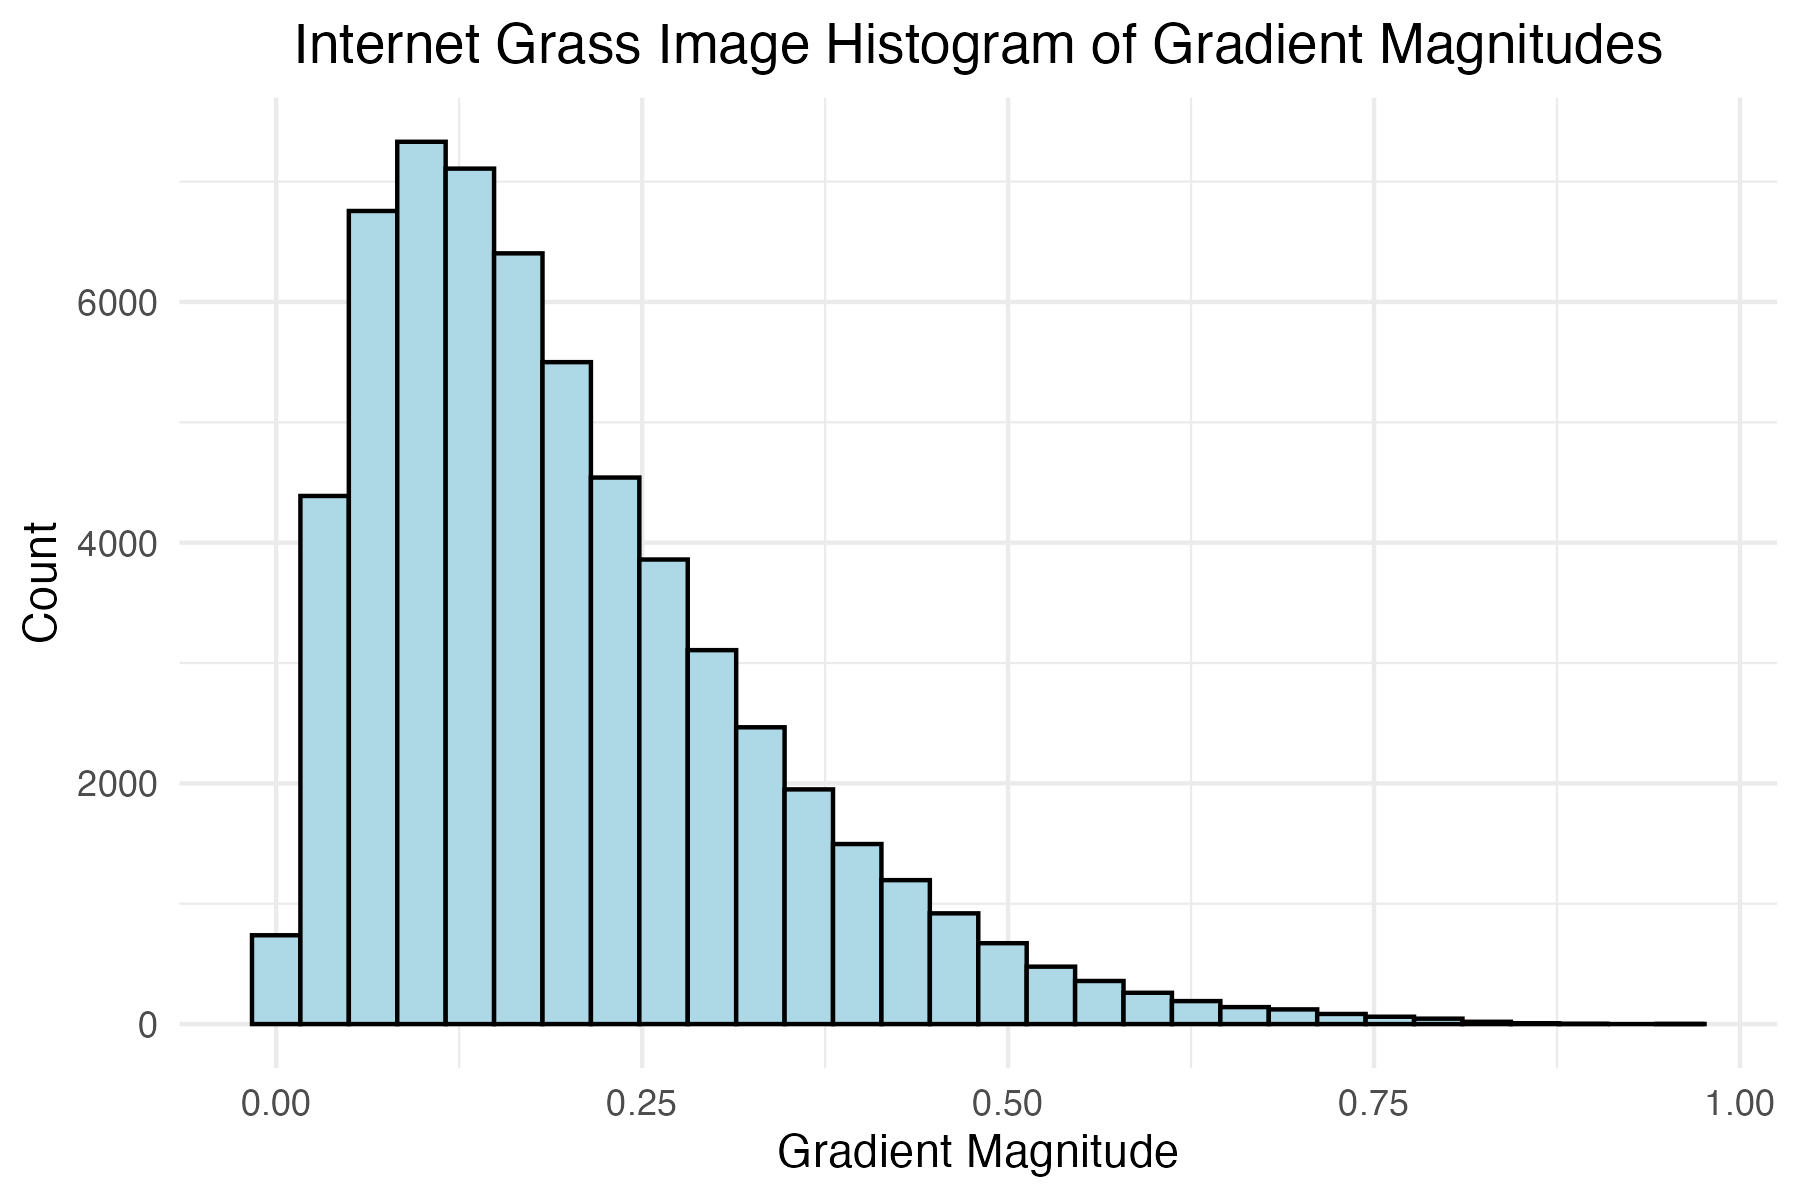
\includegraphics{images/plots/grass/internet_grass_histogram_mag_plot.jpg}
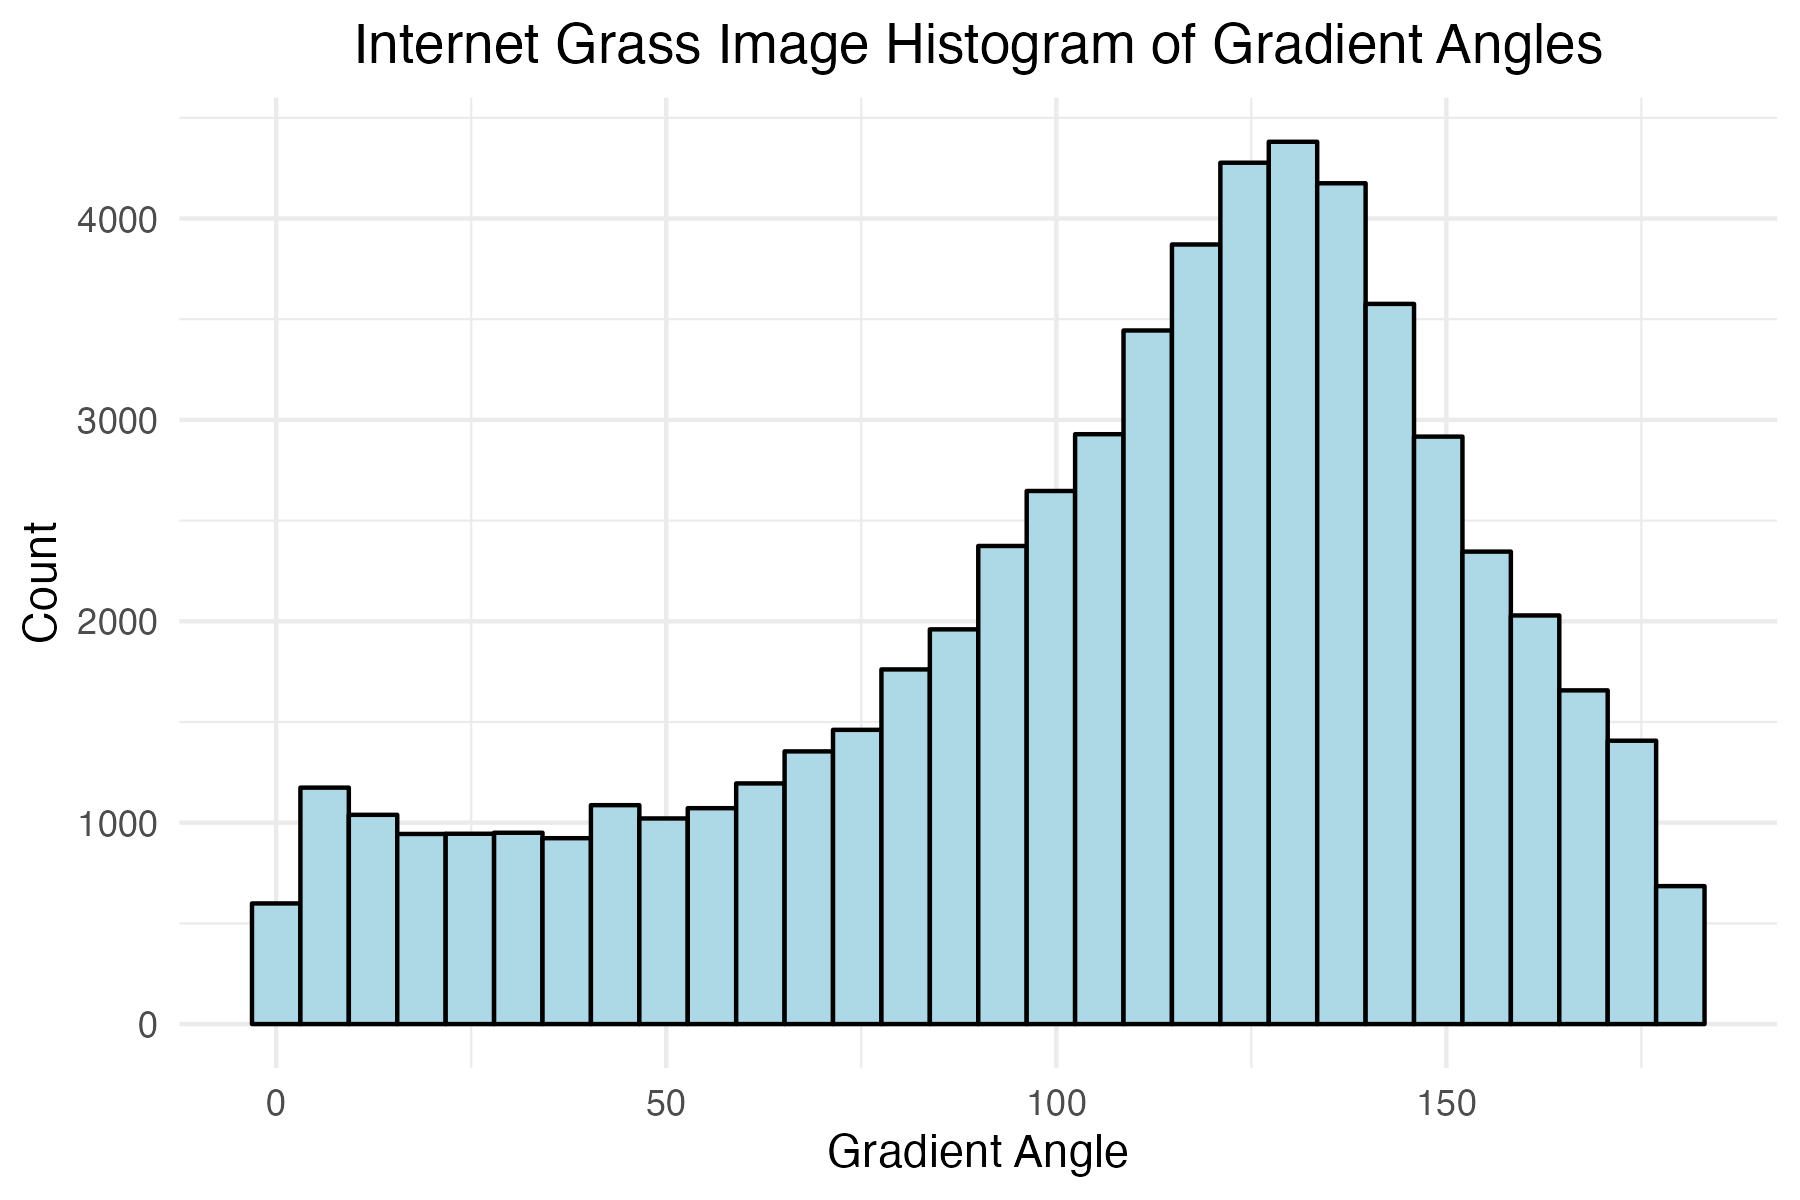
\includegraphics{images/plots/grass/internet_grass_histogram_theta_plot.jpg}\end{minipage}%
%
\begin{minipage}{0.33\linewidth}
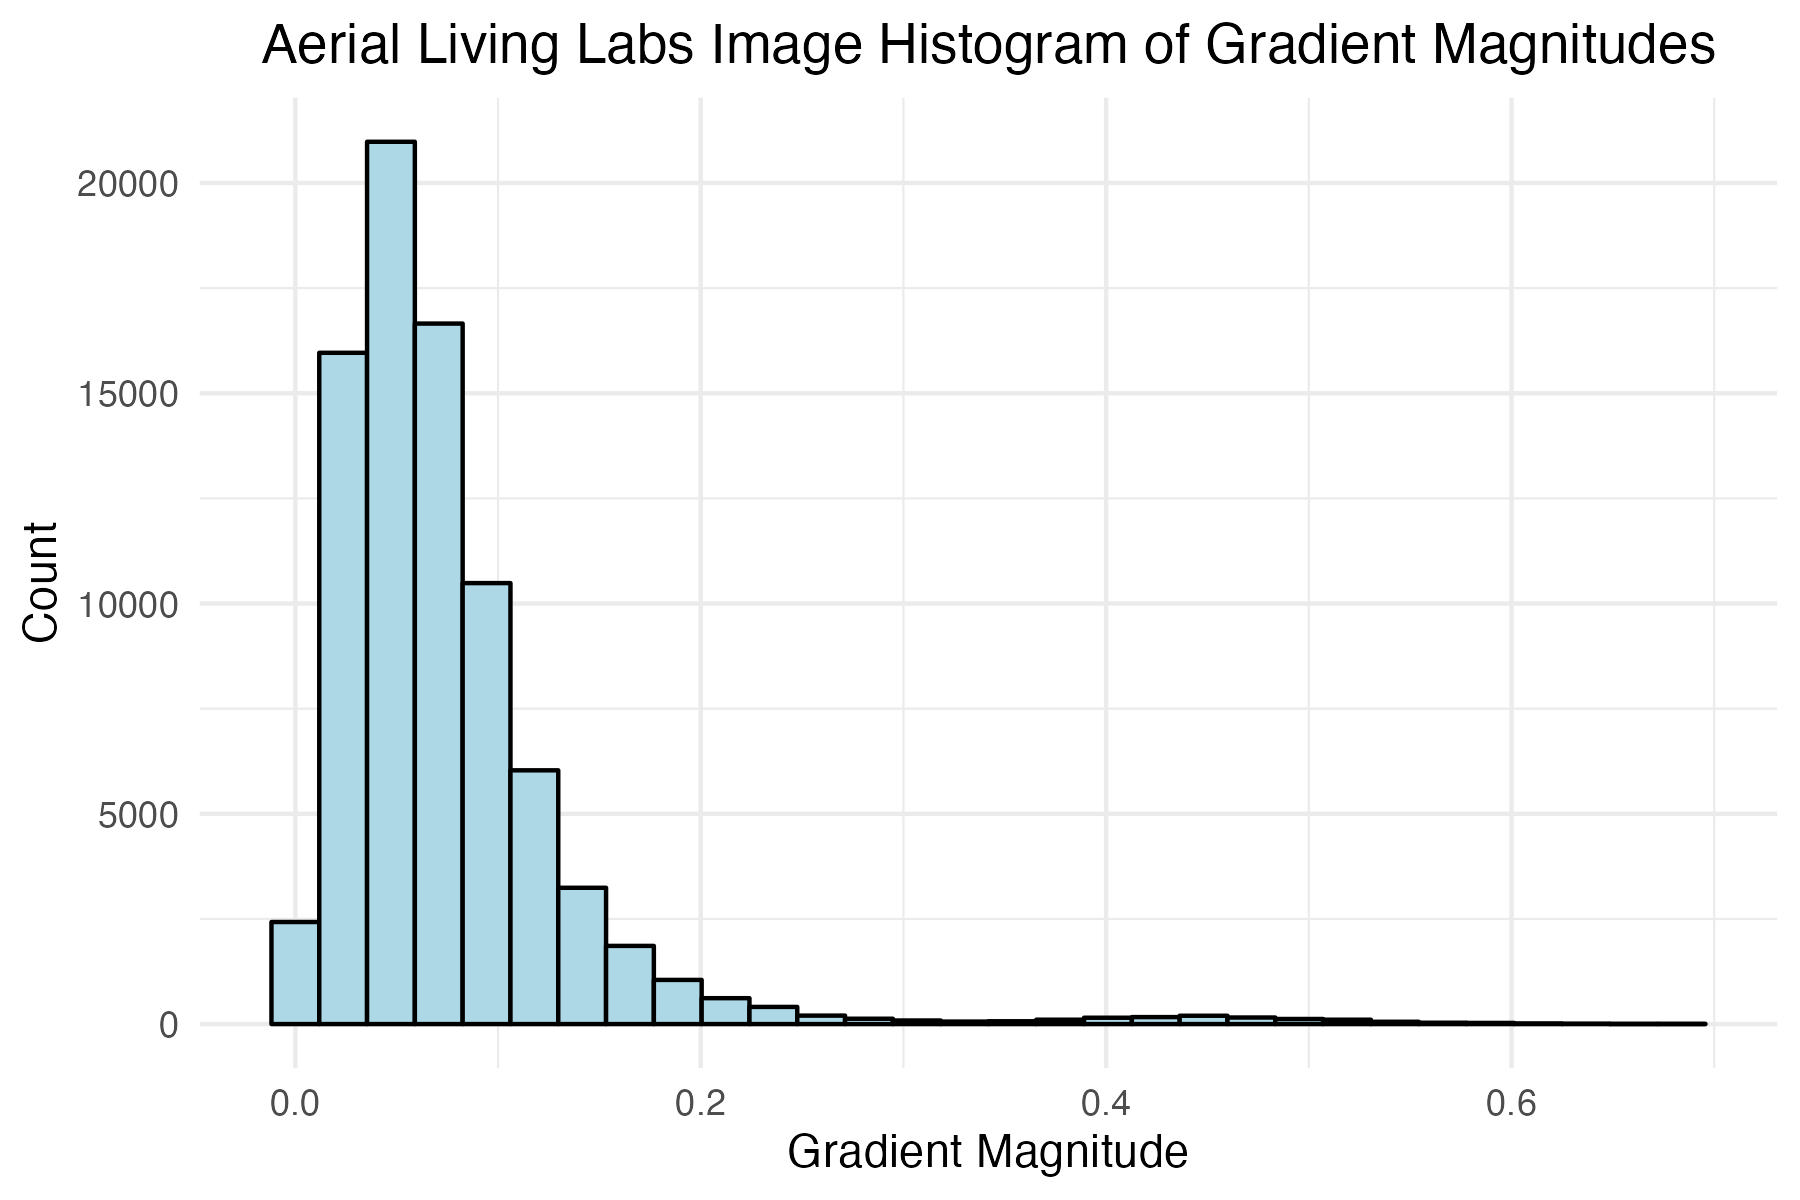
\includegraphics{images/plots/grass/aerial_living_lab_histogram_mag_plot.jpg}
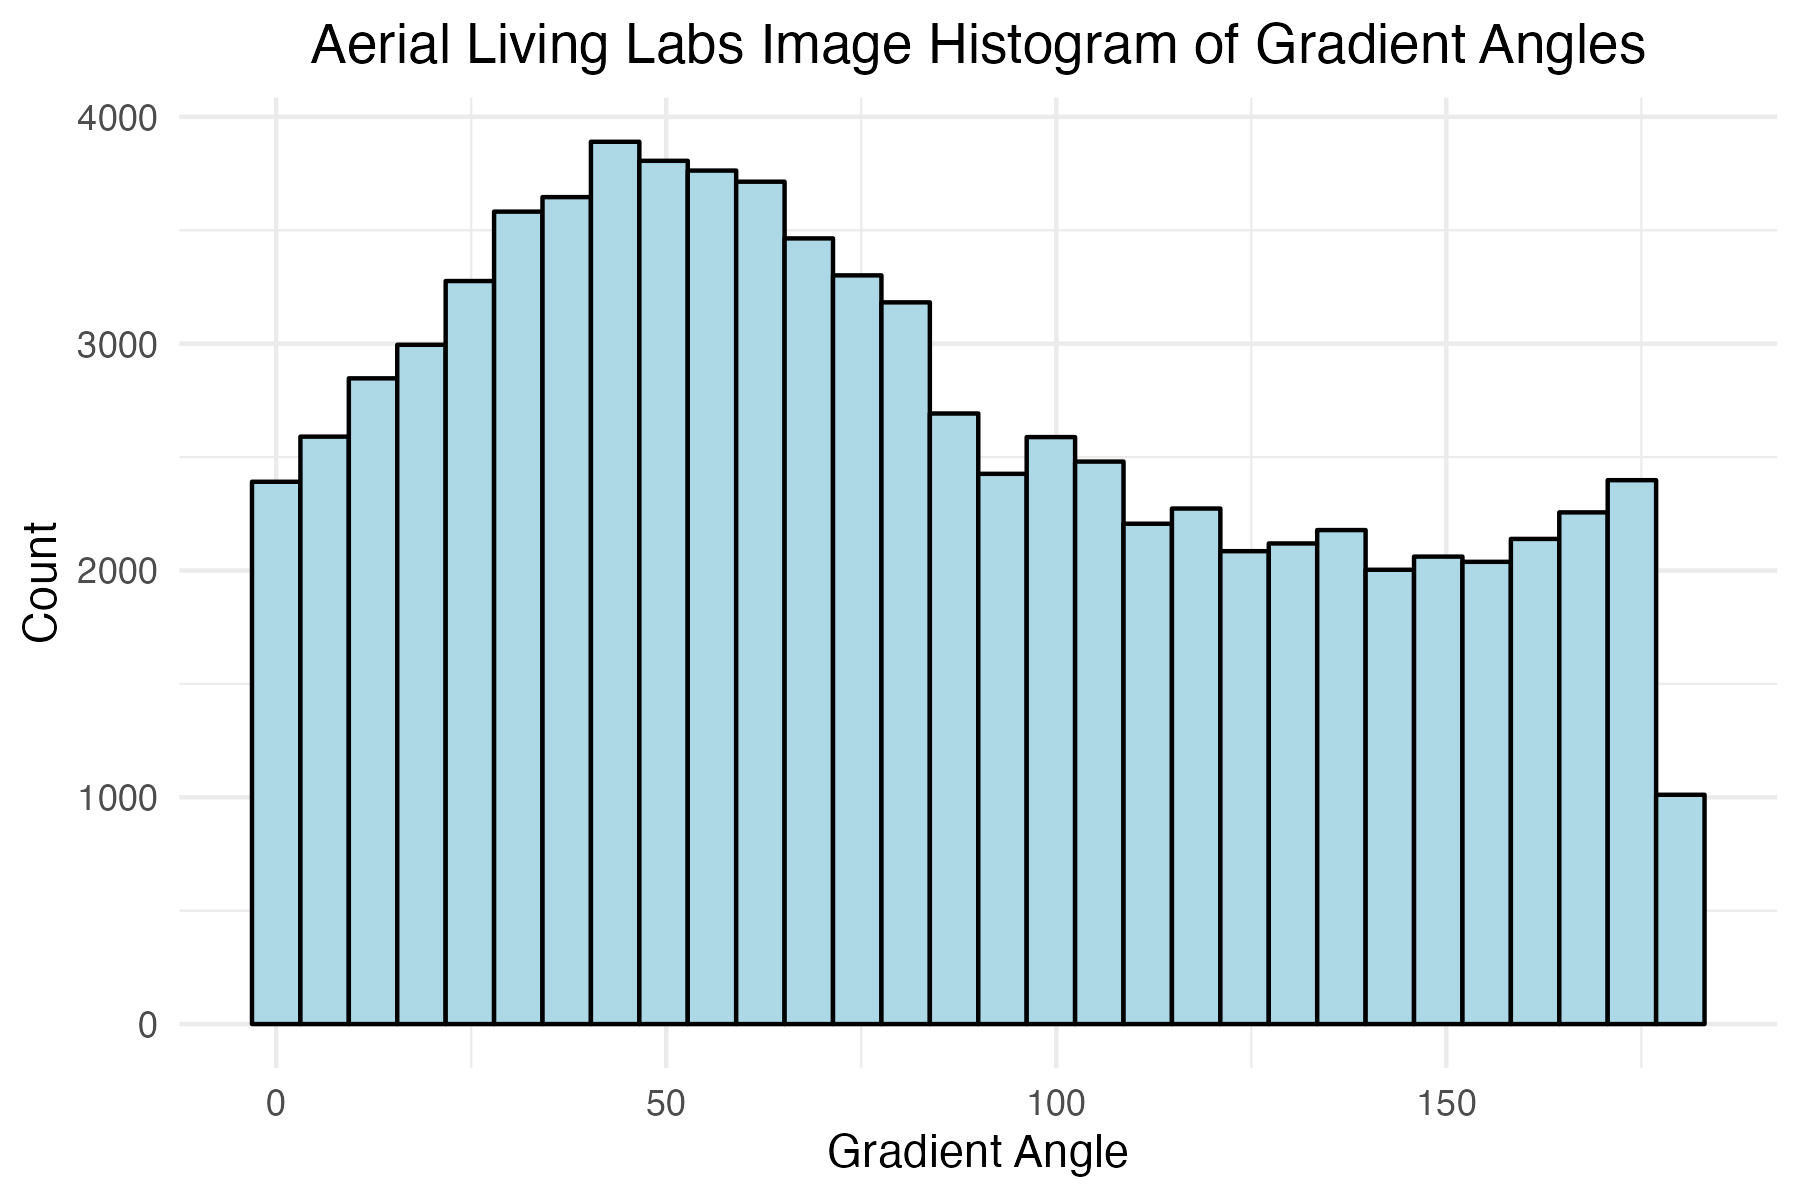
\includegraphics{images/plots/grass/aerial_living_lab_histogram_theta_plot.jpg}\end{minipage}%
%
\begin{minipage}{0.33\linewidth}
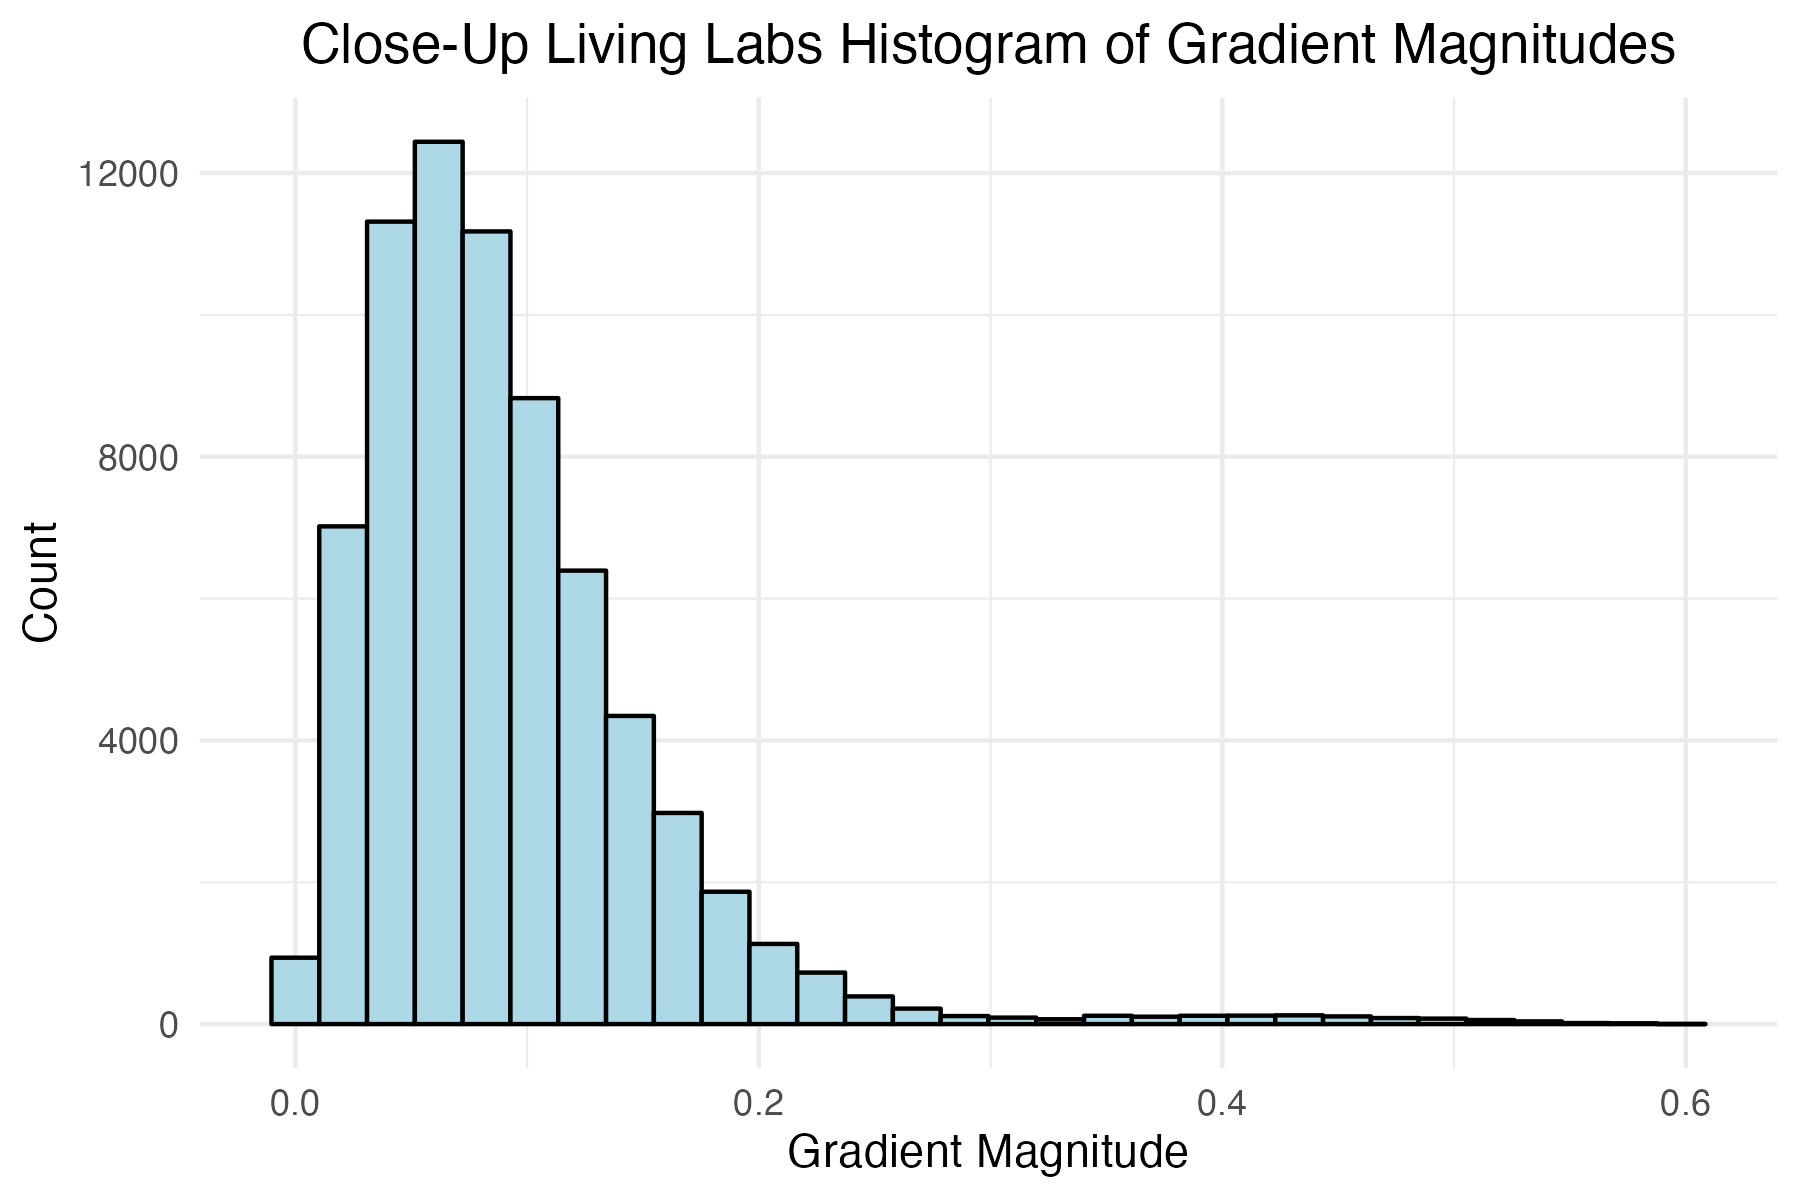
\includegraphics{images/plots/grass/close_up_living_lab_histogram_mag_plot.jpg}
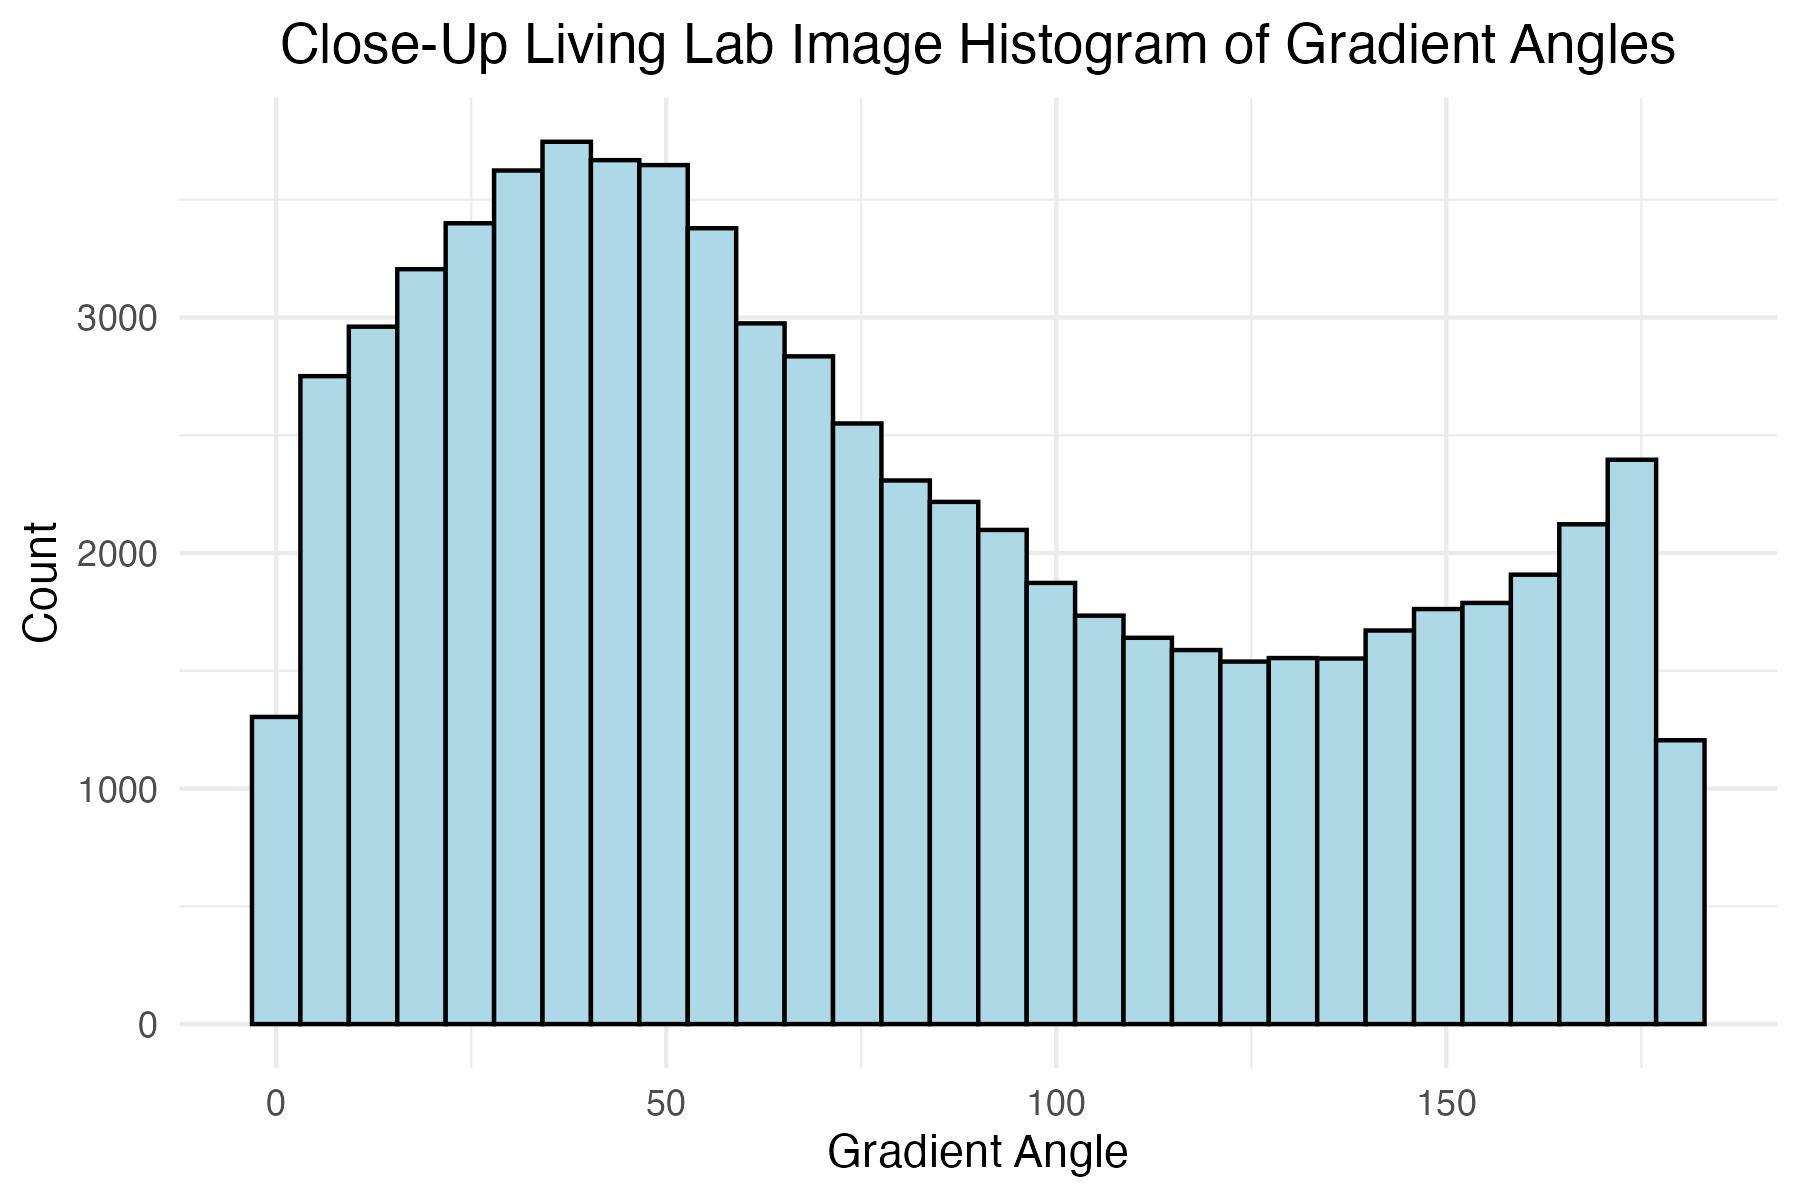
\includegraphics{images/plots/grass/close_up_living_lab_histogram_theta_plot.jpg}\end{minipage}%

\caption{\label{fig-grass-histograms}Grass Image Magnitudes and Angles}

\end{figure}%

\section{Build New Distributed Histogram Data Frames for Grass
Images}\label{build-new-distributed-histogram-data-frames-for-grass-images}

\begin{Shaded}
\begin{Highlighting}[]
\NormalTok{calculate\_bin\_contributions }\OtherTok{\textless{}{-}} \ControlFlowTok{function}\NormalTok{(angle, magnitude, num\_bins) \{}
\NormalTok{  bin\_width }\OtherTok{\textless{}{-}} \DecValTok{180} \SpecialCharTok{/}\NormalTok{ num\_bins}
\NormalTok{  contributions }\OtherTok{\textless{}{-}} \FunctionTok{numeric}\NormalTok{(num\_bins)}
  
  \CommentTok{\# get the central bin}
\NormalTok{  central\_bin }\OtherTok{\textless{}{-}} \FunctionTok{floor}\NormalTok{(angle }\SpecialCharTok{/}\NormalTok{ bin\_width) }\SpecialCharTok{\%\%}\NormalTok{ num\_bins}
\NormalTok{  next\_bin }\OtherTok{\textless{}{-}}\NormalTok{ (central\_bin }\SpecialCharTok{+} \DecValTok{1}\NormalTok{) }\SpecialCharTok{\%\%}\NormalTok{ num\_bins}
  
  \CommentTok{\# get contributions to neighboring bins}
\NormalTok{  weight }\OtherTok{\textless{}{-}}\NormalTok{ (}\DecValTok{1} \SpecialCharTok{{-}} \FunctionTok{abs}\NormalTok{((angle }\SpecialCharTok{\%\%}\NormalTok{ bin\_width) }\SpecialCharTok{/}\NormalTok{ bin\_width)) }\SpecialCharTok{*}\NormalTok{ magnitude}
  
\NormalTok{  contributions[central\_bin }\SpecialCharTok{+} \DecValTok{1}\NormalTok{] }\OtherTok{\textless{}{-}}\NormalTok{ weight}
\NormalTok{  contributions[next\_bin }\SpecialCharTok{+} \DecValTok{1}\NormalTok{] }\OtherTok{\textless{}{-}}\NormalTok{ magnitude }\SpecialCharTok{{-}}\NormalTok{ weight}
  
  \FunctionTok{return}\NormalTok{(}\FunctionTok{list}\NormalTok{(contributions[}\DecValTok{1}\NormalTok{],}
\NormalTok{         contributions[}\DecValTok{2}\NormalTok{],}
\NormalTok{         contributions[}\DecValTok{3}\NormalTok{],}
\NormalTok{         contributions[}\DecValTok{4}\NormalTok{],}
\NormalTok{         contributions[}\DecValTok{5}\NormalTok{],}
\NormalTok{         contributions[}\DecValTok{6}\NormalTok{],}
\NormalTok{         contributions[}\DecValTok{7}\NormalTok{],}
\NormalTok{         contributions[}\DecValTok{8}\NormalTok{],}
\NormalTok{         contributions[}\DecValTok{9}\NormalTok{])}
\NormalTok{         )}
\NormalTok{\}}
\end{Highlighting}
\end{Shaded}

\begin{Shaded}
\begin{Highlighting}[]
\CommentTok{\# Create filtered data frames using the filter levels for magnitudes defined above, store all in a list}
\NormalTok{filtered\_grass\_standard\_df\_list }\OtherTok{\textless{}{-}}\FunctionTok{list}\NormalTok{(internet\_grass\_hog\_df }\SpecialCharTok{\%\textgreater{}\%}
                                          \FunctionTok{filter}\NormalTok{(mag }\SpecialCharTok{\textgreater{}=}\NormalTok{ internet\_grass\_mag\_filter),}
\NormalTok{                                        aerial\_living\_lab\_hog\_df }\SpecialCharTok{\%\textgreater{}\%}
                                          \FunctionTok{filter}\NormalTok{(mag }\SpecialCharTok{\textgreater{}=}\NormalTok{ aerial\_living\_lab\_mag\_filter), }
\NormalTok{                                        close\_up\_living\_lab\_hog\_df }\SpecialCharTok{\%\textgreater{}\%}
                                          \FunctionTok{filter}\NormalTok{(mag }\SpecialCharTok{\textgreater{}=}\NormalTok{ close\_up\_living\_lab\_mag\_filter))}
\end{Highlighting}
\end{Shaded}

\begin{Shaded}
\begin{Highlighting}[]
\CommentTok{\# empty list for storing new distributed histogram data frames}
\NormalTok{grass\_contribution\_df\_list }\OtherTok{\textless{}{-}} \FunctionTok{list}\NormalTok{()}

\CommentTok{\# Define the number of bins}
\NormalTok{num\_bins }\OtherTok{\textless{}{-}} \DecValTok{9}

\CommentTok{\# iterate through each filtered standard data frame}
\ControlFlowTok{for}\NormalTok{ (i }\ControlFlowTok{in} \DecValTok{1}\SpecialCharTok{:}\FunctionTok{length}\NormalTok{(filtered\_grass\_standard\_df\_list))\{}
  
\NormalTok{  grass\_contribution\_hog\_df }\OtherTok{\textless{}{-}} 
\NormalTok{    filtered\_grass\_standard\_df\_list[[i]] }\SpecialCharTok{\%\textgreater{}\%}
    \FunctionTok{rowwise}\NormalTok{() }\SpecialCharTok{\%\textgreater{}\%}
    \FunctionTok{mutate}\NormalTok{(}\StringTok{\textasciigrave{}}\AttributeTok{0}\StringTok{\textasciigrave{}} \OtherTok{=} \FunctionTok{calculate\_bin\_contributions}\NormalTok{(theta, mag, }\DecValTok{9}\NormalTok{)[[}\DecValTok{1}\NormalTok{]],}
           \StringTok{\textasciigrave{}}\AttributeTok{20}\StringTok{\textasciigrave{}} \OtherTok{=} \FunctionTok{calculate\_bin\_contributions}\NormalTok{(theta, mag, }\DecValTok{9}\NormalTok{)[[}\DecValTok{2}\NormalTok{]],}
           \StringTok{\textasciigrave{}}\AttributeTok{40}\StringTok{\textasciigrave{}} \OtherTok{=} \FunctionTok{calculate\_bin\_contributions}\NormalTok{(theta, mag, }\DecValTok{9}\NormalTok{)[[}\DecValTok{3}\NormalTok{]],}
           \StringTok{\textasciigrave{}}\AttributeTok{60}\StringTok{\textasciigrave{}} \OtherTok{=} \FunctionTok{calculate\_bin\_contributions}\NormalTok{(theta, mag, }\DecValTok{9}\NormalTok{)[[}\DecValTok{4}\NormalTok{]],}
           \StringTok{\textasciigrave{}}\AttributeTok{80}\StringTok{\textasciigrave{}} \OtherTok{=} \FunctionTok{calculate\_bin\_contributions}\NormalTok{(theta, mag, }\DecValTok{9}\NormalTok{)[[}\DecValTok{5}\NormalTok{]],}
           \StringTok{\textasciigrave{}}\AttributeTok{100}\StringTok{\textasciigrave{}} \OtherTok{=} \FunctionTok{calculate\_bin\_contributions}\NormalTok{(theta, mag, }\DecValTok{9}\NormalTok{)[[}\DecValTok{6}\NormalTok{]],}
           \StringTok{\textasciigrave{}}\AttributeTok{120}\StringTok{\textasciigrave{}} \OtherTok{=} \FunctionTok{calculate\_bin\_contributions}\NormalTok{(theta, mag, }\DecValTok{9}\NormalTok{)[[}\DecValTok{7}\NormalTok{]],}
           \StringTok{\textasciigrave{}}\AttributeTok{140}\StringTok{\textasciigrave{}} \OtherTok{=} \FunctionTok{calculate\_bin\_contributions}\NormalTok{(theta, mag, }\DecValTok{9}\NormalTok{)[[}\DecValTok{8}\NormalTok{]],}
           \StringTok{\textasciigrave{}}\AttributeTok{160}\StringTok{\textasciigrave{}} \OtherTok{=} \FunctionTok{calculate\_bin\_contributions}\NormalTok{(theta, mag, }\DecValTok{9}\NormalTok{)[[}\DecValTok{9}\NormalTok{]],}
\NormalTok{           )}
  
    \CommentTok{\# rearrange into same tidy format}
\NormalTok{  grass\_split\_histo\_df }\OtherTok{\textless{}{-}} 
\NormalTok{    grass\_contribution\_hog\_df }\SpecialCharTok{\%\textgreater{}\%}
    \FunctionTok{pivot\_longer}\NormalTok{(}\AttributeTok{names\_to =} \StringTok{"bin"}\NormalTok{, }
                 \AttributeTok{values\_to =} \StringTok{"contribution"}\NormalTok{, }
                 \AttributeTok{cols =} \DecValTok{4}\SpecialCharTok{:}\FunctionTok{ncol}\NormalTok{(grass\_contribution\_hog\_df)) }\SpecialCharTok{\%\textgreater{}\%}
    \FunctionTok{mutate}\NormalTok{(}\AttributeTok{bin =} \FunctionTok{as.numeric}\NormalTok{(bin)) }\SpecialCharTok{\%\textgreater{}\%}
    \FunctionTok{group\_by}\NormalTok{(bin) }\SpecialCharTok{\%\textgreater{}\%}
    \FunctionTok{summarise}\NormalTok{(}\AttributeTok{contribution\_sum =} \FunctionTok{sum}\NormalTok{(contribution))}
  
  \CommentTok{\# add to list for storage}
\NormalTok{  grass\_contribution\_df\_list[[i]] }\OtherTok{\textless{}{-}}\NormalTok{ grass\_split\_histo\_df}

\NormalTok{\}}
\end{Highlighting}
\end{Shaded}

\section{Generate Polar Plots for Images Using Standard Histogram
Binning
Technique}\label{generate-polar-plots-for-images-using-standard-histogram-binning-technique-1}

\begin{Shaded}
\begin{Highlighting}[]
\CommentTok{\# Internet grass plot}
\NormalTok{internet\_grass\_plot }\OtherTok{\textless{}{-}}
  \FunctionTok{ggplot}\NormalTok{(filtered\_grass\_standard\_df\_list[[}\DecValTok{1}\NormalTok{]], }
         \FunctionTok{aes}\NormalTok{(}\AttributeTok{x =}\NormalTok{ theta)) }\SpecialCharTok{+}
  \FunctionTok{geom\_histogram}\NormalTok{(}\AttributeTok{colour =} \StringTok{"black"}\NormalTok{, }
                 \AttributeTok{fill =} \StringTok{"lightblue"}\NormalTok{, }
                 \AttributeTok{breaks =} \FunctionTok{seq}\NormalTok{(}\DecValTok{0}\NormalTok{, }\DecValTok{360}\NormalTok{, }\AttributeTok{length.out =} \FloatTok{17.5}\NormalTok{),}
                 \AttributeTok{bins =} \DecValTok{9}\NormalTok{) }\SpecialCharTok{+}
  \FunctionTok{coord\_polar}\NormalTok{(}
    \AttributeTok{theta =} \StringTok{"x"}\NormalTok{, }
    \AttributeTok{start =} \DecValTok{0}\NormalTok{, }
    \AttributeTok{direction =} \DecValTok{1}\NormalTok{) }\SpecialCharTok{+}
  \FunctionTok{scale\_x\_continuous}\NormalTok{(}\AttributeTok{limits =} \FunctionTok{c}\NormalTok{(}\DecValTok{0}\NormalTok{,}\DecValTok{360}\NormalTok{),}
    \AttributeTok{breaks =} \FunctionTok{c}\NormalTok{(}\DecValTok{0}\NormalTok{, }\DecValTok{45}\NormalTok{, }\DecValTok{90}\NormalTok{, }\DecValTok{135}\NormalTok{, }\DecValTok{180}\NormalTok{, }\DecValTok{225}\NormalTok{, }\DecValTok{270}\NormalTok{, }\DecValTok{315}\NormalTok{), }
    \AttributeTok{labels =} \FunctionTok{c}\NormalTok{(}\StringTok{"N"}\NormalTok{, }\StringTok{"NE"}\NormalTok{, }\StringTok{"E"}\NormalTok{, }\StringTok{"SE"}\NormalTok{, }\StringTok{"S"}\NormalTok{, }\StringTok{"SW"}\NormalTok{, }\StringTok{"W"}\NormalTok{, }\StringTok{"NW"}\NormalTok{)}
\NormalTok{  )}\SpecialCharTok{+}
  \FunctionTok{labs}\NormalTok{(}\AttributeTok{title =} \StringTok{"Polar Plot of Internet Grass Image}\SpecialCharTok{\textbackslash{}n}\StringTok{Using Standard HOG Technique"}\NormalTok{) }\SpecialCharTok{+}
  \FunctionTok{theme\_minimal}\NormalTok{() }\SpecialCharTok{+}
  \FunctionTok{labs}\NormalTok{(}\AttributeTok{x =} \StringTok{""}\NormalTok{) }\SpecialCharTok{+}
  \FunctionTok{theme}\NormalTok{(}\AttributeTok{axis.title.y =} \FunctionTok{element\_blank}\NormalTok{(),}
        \AttributeTok{plot.title =} \FunctionTok{element\_text}\NormalTok{(}\AttributeTok{hjust =} \FloatTok{0.5}\NormalTok{))}

\CommentTok{\# save image}
\FunctionTok{ggsave}\NormalTok{(}\StringTok{"images/plots/grass/internet\_grass\_standard\_polar\_plot.jpg"}\NormalTok{, internet\_grass\_plot, }\AttributeTok{width =} \DecValTok{6}\NormalTok{, }\AttributeTok{height =} \DecValTok{4}\NormalTok{, }\AttributeTok{dpi =} \DecValTok{300}\NormalTok{)}
\end{Highlighting}
\end{Shaded}

\begin{Shaded}
\begin{Highlighting}[]
\CommentTok{\# Aerial Living Labs plot}
\NormalTok{aerial\_living\_lab\_plot }\OtherTok{\textless{}{-}}
  \FunctionTok{ggplot}\NormalTok{(filtered\_grass\_standard\_df\_list[[}\DecValTok{2}\NormalTok{]], }
         \FunctionTok{aes}\NormalTok{(}\AttributeTok{x =}\NormalTok{ theta)) }\SpecialCharTok{+}
  \FunctionTok{geom\_histogram}\NormalTok{(}\AttributeTok{colour =} \StringTok{"black"}\NormalTok{, }
                 \AttributeTok{fill =} \StringTok{"lightblue"}\NormalTok{, }
                 \AttributeTok{breaks =} \FunctionTok{seq}\NormalTok{(}\DecValTok{0}\NormalTok{, }\DecValTok{360}\NormalTok{, }\AttributeTok{length.out =} \FloatTok{17.5}\NormalTok{),}
                 \AttributeTok{bins =} \DecValTok{9}\NormalTok{) }\SpecialCharTok{+}
  \FunctionTok{coord\_polar}\NormalTok{(}
    \AttributeTok{theta =} \StringTok{"x"}\NormalTok{, }
    \AttributeTok{start =} \DecValTok{0}\NormalTok{, }
    \AttributeTok{direction =} \DecValTok{1}\NormalTok{) }\SpecialCharTok{+}
  \FunctionTok{scale\_x\_continuous}\NormalTok{(}\AttributeTok{limits =} \FunctionTok{c}\NormalTok{(}\DecValTok{0}\NormalTok{,}\DecValTok{360}\NormalTok{),}
    \AttributeTok{breaks =} \FunctionTok{c}\NormalTok{(}\DecValTok{0}\NormalTok{, }\DecValTok{45}\NormalTok{, }\DecValTok{90}\NormalTok{, }\DecValTok{135}\NormalTok{, }\DecValTok{180}\NormalTok{, }\DecValTok{225}\NormalTok{, }\DecValTok{270}\NormalTok{, }\DecValTok{315}\NormalTok{), }
    \AttributeTok{labels =} \FunctionTok{c}\NormalTok{(}\StringTok{"N"}\NormalTok{, }\StringTok{"NE"}\NormalTok{, }\StringTok{"E"}\NormalTok{, }\StringTok{"SE"}\NormalTok{, }\StringTok{"S"}\NormalTok{, }\StringTok{"SW"}\NormalTok{, }\StringTok{"W"}\NormalTok{, }\StringTok{"NW"}\NormalTok{)}
\NormalTok{  )}\SpecialCharTok{+}
  \FunctionTok{labs}\NormalTok{(}\AttributeTok{title =} \StringTok{"Polar Plot of Aerial Living Labs Image}\SpecialCharTok{\textbackslash{}n}\StringTok{Using Standard HOG Technique"}\NormalTok{) }\SpecialCharTok{+}
  \FunctionTok{theme\_minimal}\NormalTok{() }\SpecialCharTok{+}
  \FunctionTok{labs}\NormalTok{(}\AttributeTok{x =} \StringTok{""}\NormalTok{) }\SpecialCharTok{+}
  \FunctionTok{theme}\NormalTok{(}\AttributeTok{axis.title.y =} \FunctionTok{element\_blank}\NormalTok{(),}
        \AttributeTok{plot.title =} \FunctionTok{element\_text}\NormalTok{(}\AttributeTok{hjust =} \FloatTok{0.5}\NormalTok{))}

\CommentTok{\# save image}
\FunctionTok{ggsave}\NormalTok{(}\StringTok{"images/plots/grass/aerial\_living\_lab\_standard\_polar\_plot.jpg"}\NormalTok{, aerial\_living\_lab\_plot, }\AttributeTok{width =} \DecValTok{6}\NormalTok{, }\AttributeTok{height =} \DecValTok{4}\NormalTok{, }\AttributeTok{dpi =} \DecValTok{300}\NormalTok{)}
\end{Highlighting}
\end{Shaded}

\begin{Shaded}
\begin{Highlighting}[]
\CommentTok{\# Close{-}up Living Labs plot}
\NormalTok{close\_up\_living\_lab\_plot }\OtherTok{\textless{}{-}}
  \FunctionTok{ggplot}\NormalTok{(filtered\_grass\_standard\_df\_list[[}\DecValTok{3}\NormalTok{]], }
         \FunctionTok{aes}\NormalTok{(}\AttributeTok{x =}\NormalTok{ theta)) }\SpecialCharTok{+}
  \FunctionTok{geom\_histogram}\NormalTok{(}\AttributeTok{colour =} \StringTok{"black"}\NormalTok{, }
                 \AttributeTok{fill =} \StringTok{"lightblue"}\NormalTok{, }
                 \AttributeTok{breaks =} \FunctionTok{seq}\NormalTok{(}\DecValTok{0}\NormalTok{, }\DecValTok{360}\NormalTok{, }\AttributeTok{length.out =} \FloatTok{17.5}\NormalTok{),}
                 \AttributeTok{bins =} \DecValTok{9}\NormalTok{) }\SpecialCharTok{+}
  \FunctionTok{coord\_polar}\NormalTok{(}
    \AttributeTok{theta =} \StringTok{"x"}\NormalTok{, }
    \AttributeTok{start =} \DecValTok{0}\NormalTok{, }
    \AttributeTok{direction =} \DecValTok{1}\NormalTok{) }\SpecialCharTok{+}
  \FunctionTok{scale\_x\_continuous}\NormalTok{(}\AttributeTok{limits =} \FunctionTok{c}\NormalTok{(}\DecValTok{0}\NormalTok{,}\DecValTok{360}\NormalTok{),}
    \AttributeTok{breaks =} \FunctionTok{c}\NormalTok{(}\DecValTok{0}\NormalTok{, }\DecValTok{45}\NormalTok{, }\DecValTok{90}\NormalTok{, }\DecValTok{135}\NormalTok{, }\DecValTok{180}\NormalTok{, }\DecValTok{225}\NormalTok{, }\DecValTok{270}\NormalTok{, }\DecValTok{315}\NormalTok{), }
    \AttributeTok{labels =} \FunctionTok{c}\NormalTok{(}\StringTok{"N"}\NormalTok{, }\StringTok{"NE"}\NormalTok{, }\StringTok{"E"}\NormalTok{, }\StringTok{"SE"}\NormalTok{, }\StringTok{"S"}\NormalTok{, }\StringTok{"SW"}\NormalTok{, }\StringTok{"W"}\NormalTok{, }\StringTok{"NW"}\NormalTok{)}
\NormalTok{  )}\SpecialCharTok{+}
  \FunctionTok{labs}\NormalTok{(}\AttributeTok{title =} \StringTok{"Polar Plot of Close{-}Up Living Lab Image}\SpecialCharTok{\textbackslash{}n}\StringTok{Using Standard HOG Technique"}\NormalTok{) }\SpecialCharTok{+}
  \FunctionTok{theme\_minimal}\NormalTok{() }\SpecialCharTok{+}
  \FunctionTok{labs}\NormalTok{(}\AttributeTok{x =} \StringTok{""}\NormalTok{) }\SpecialCharTok{+}
  \FunctionTok{theme}\NormalTok{(}\AttributeTok{axis.title.y =} \FunctionTok{element\_blank}\NormalTok{(),}
        \AttributeTok{plot.title =} \FunctionTok{element\_text}\NormalTok{(}\AttributeTok{hjust =} \FloatTok{0.5}\NormalTok{))}

\CommentTok{\# save image}
\FunctionTok{ggsave}\NormalTok{(}\StringTok{"images/plots/grass/close\_up\_living\_lab\_standard\_polar\_plot.jpg"}\NormalTok{, close\_up\_living\_lab\_plot, }\AttributeTok{width =} \DecValTok{6}\NormalTok{, }\AttributeTok{height =} \DecValTok{4}\NormalTok{, }\AttributeTok{dpi =} \DecValTok{300}\NormalTok{)}
\end{Highlighting}
\end{Shaded}

\begin{Shaded}
\begin{Highlighting}[]
\CommentTok{\# Save to an arranged image}
\NormalTok{all\_standard\_grass\_plots }\OtherTok{\textless{}{-}}\NormalTok{ ggpubr}\SpecialCharTok{::}\FunctionTok{ggarrange}\NormalTok{(internet\_grass\_plot, }
\NormalTok{                                             aerial\_living\_lab\_plot, }
\NormalTok{                                             close\_up\_living\_lab\_plot)}

\FunctionTok{ggsave}\NormalTok{(}\StringTok{"images/plots/grass/all\_grass\_standard\_polar\_plots.jpg"}\NormalTok{, }
\NormalTok{       all\_standard\_grass\_plots, }
       \AttributeTok{width =} \DecValTok{7}\NormalTok{, }
       \AttributeTok{height =} \DecValTok{7}\NormalTok{)}
\end{Highlighting}
\end{Shaded}

\begin{figure}

\begin{minipage}{0.33\linewidth}

\begin{figure}[H]

{\centering 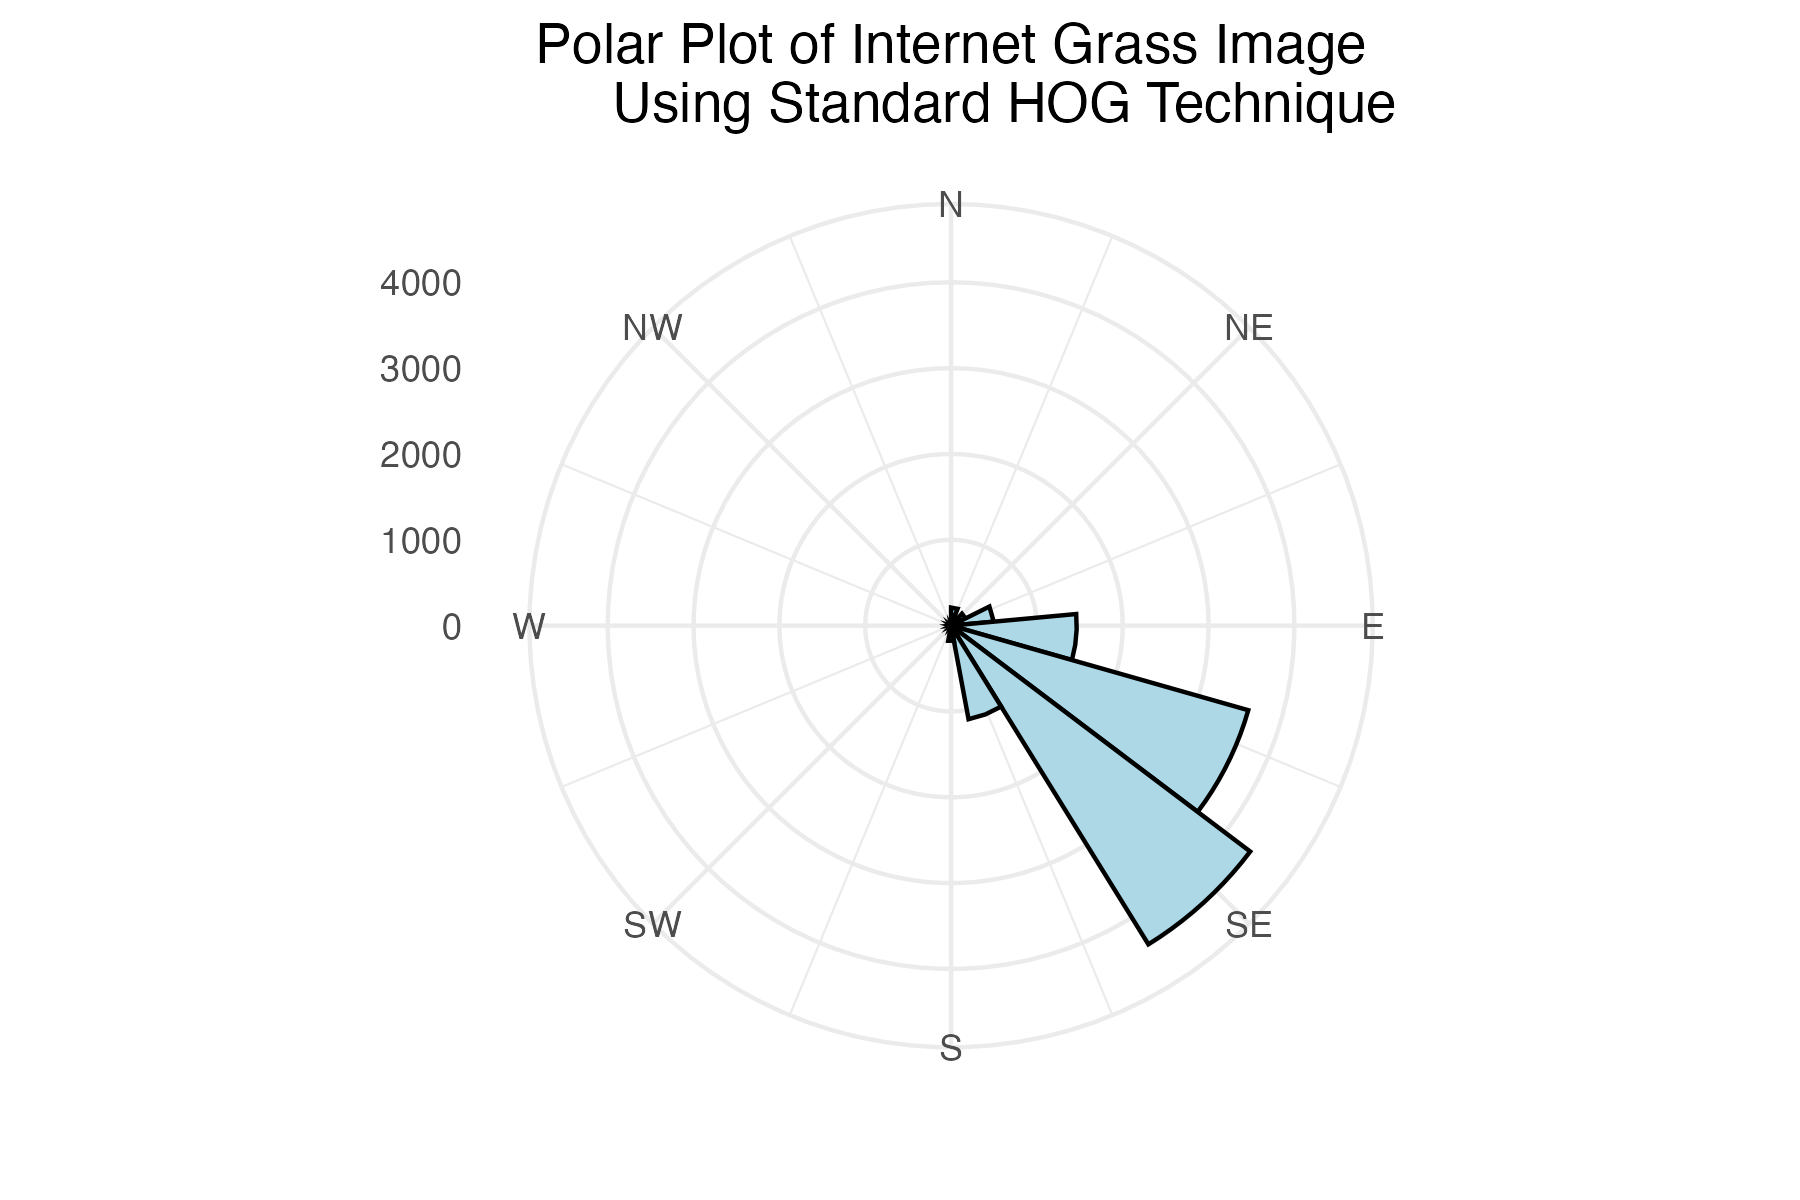
\includegraphics{images/plots/grass/internet_grass_standard_polar_plot.jpg}

}

\subcaption{Internet Grass Image}

\end{figure}%

\end{minipage}%
%
\begin{minipage}{0.33\linewidth}

\begin{figure}[H]

{\centering 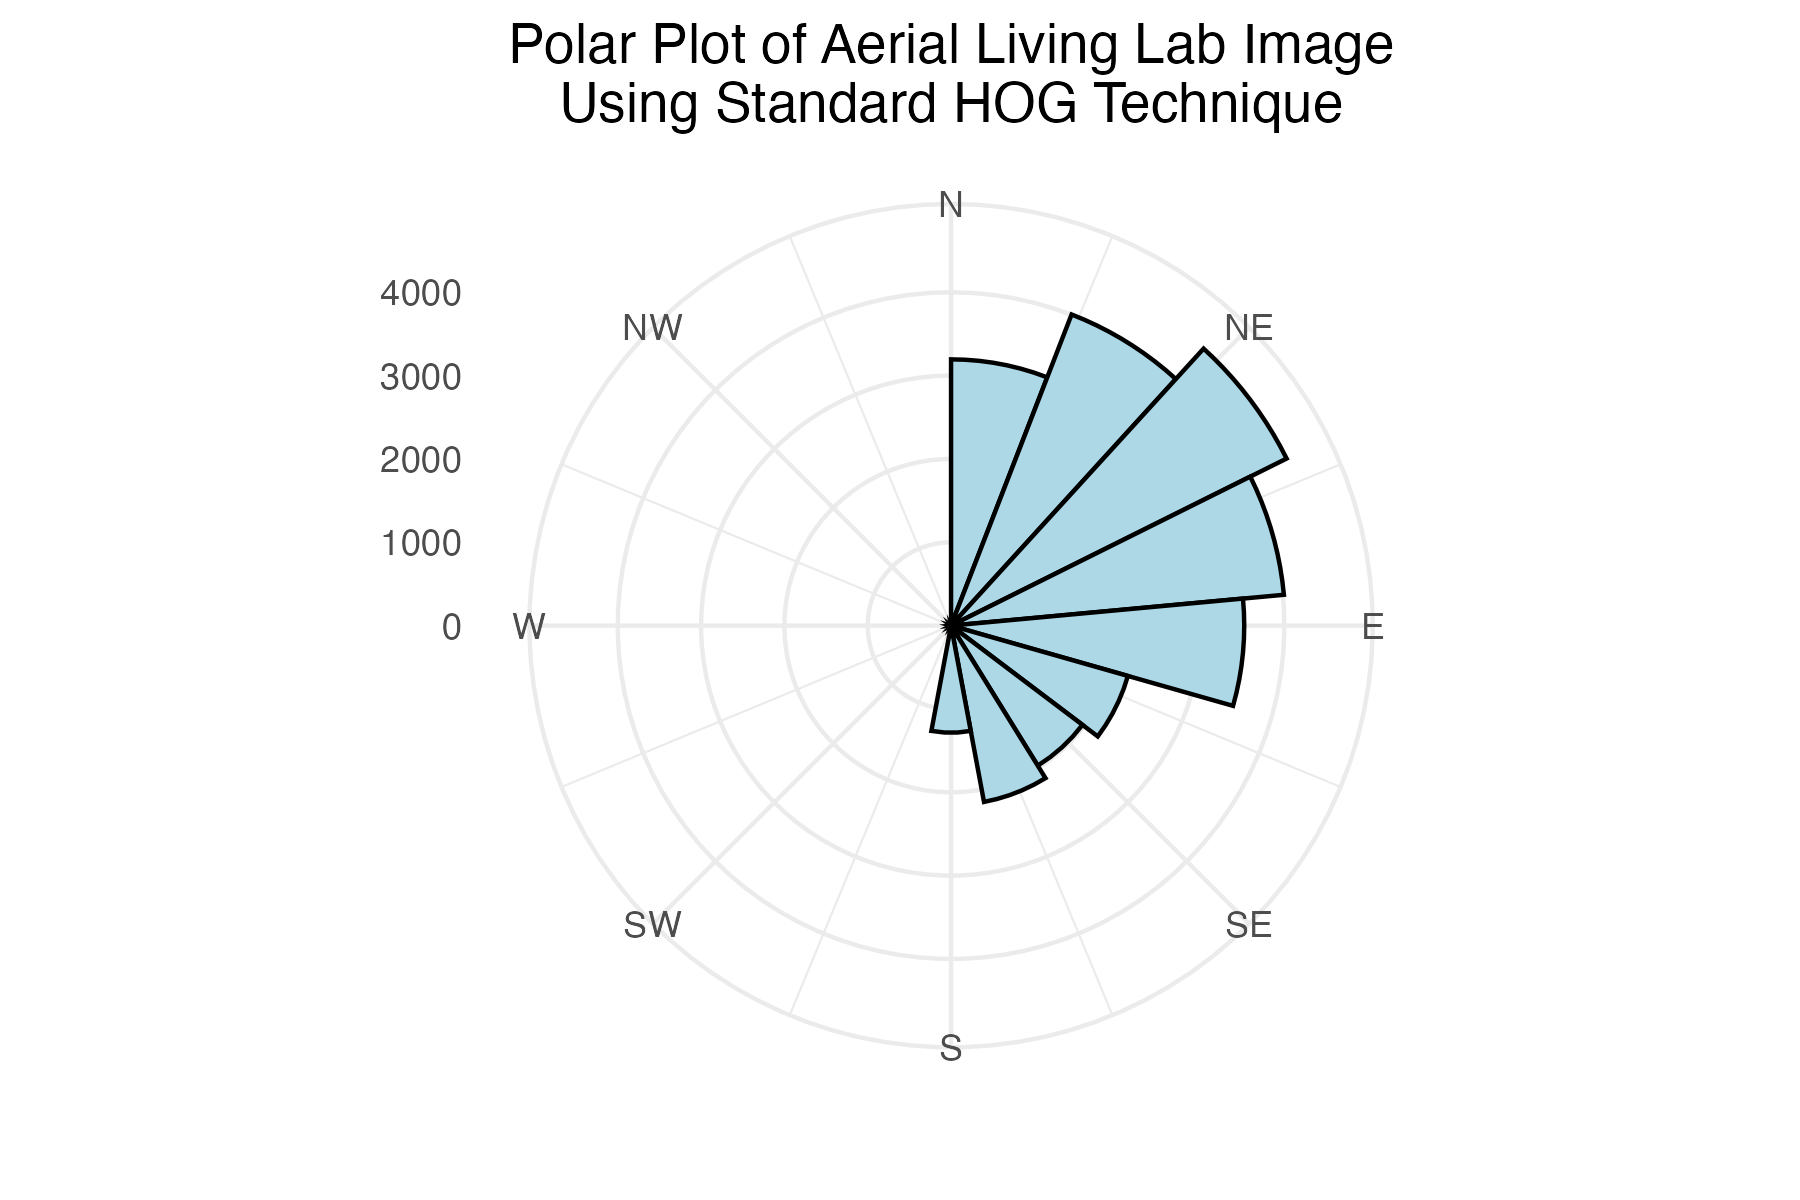
\includegraphics{images/plots/grass/aerial_living_lab_standard_polar_plot.jpg}

}

\subcaption{Aerial Living Labs Image}

\end{figure}%

\end{minipage}%
%
\begin{minipage}{0.33\linewidth}

\begin{figure}[H]

{\centering 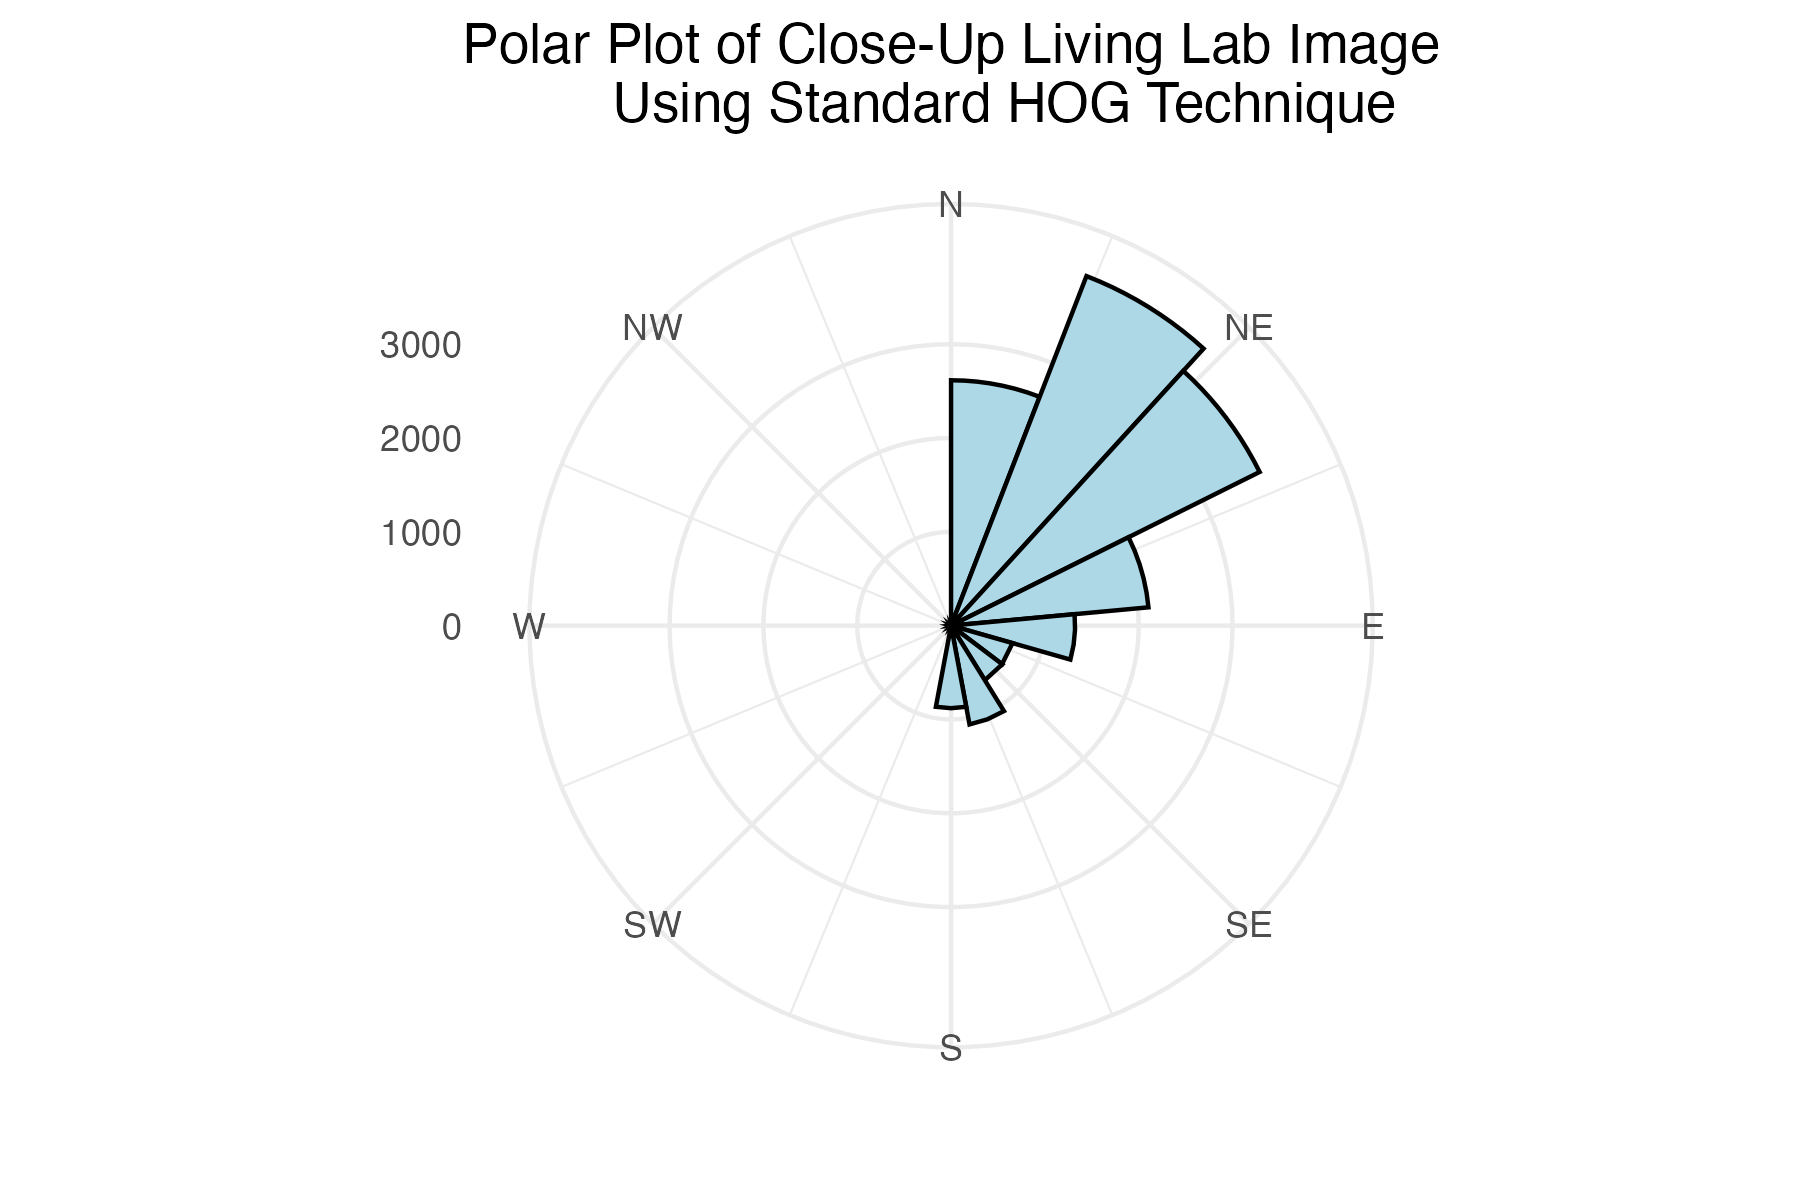
\includegraphics{images/plots/grass/close_up_living_lab_standard_polar_plot.jpg}

}

\subcaption{Close-Up Living Labs Image}

\end{figure}%

\end{minipage}%

\caption{\label{fig-grass-standard-polar}Aerial Cityscape Standard Polar
Plots}

\end{figure}%

\section{Generate Polar Plots for Images Using Distributed Histogram
Binning
Technique}\label{generate-polar-plots-for-images-using-distributed-histogram-binning-technique-1}

\begin{Shaded}
\begin{Highlighting}[]
\CommentTok{\# Internet grass plot}
\NormalTok{internet\_grass\_split\_plot }\OtherTok{\textless{}{-}}
  \FunctionTok{ggplot}\NormalTok{(grass\_contribution\_df\_list[[}\DecValTok{1}\NormalTok{]], }
         \FunctionTok{aes}\NormalTok{(}\AttributeTok{x =}\NormalTok{ bin, }\AttributeTok{y =}\NormalTok{ contribution\_sum)) }\SpecialCharTok{+}
  \FunctionTok{geom\_histogram}\NormalTok{(}\AttributeTok{stat =} \StringTok{"identity"}\NormalTok{,}
                 \AttributeTok{colour =} \StringTok{"black"}\NormalTok{, }
                 \AttributeTok{fill =} \StringTok{"lightblue"}\NormalTok{, }
                 \AttributeTok{breaks =} \FunctionTok{seq}\NormalTok{(}\DecValTok{0}\NormalTok{, }\DecValTok{360}\NormalTok{, }\AttributeTok{length.out =} \FloatTok{17.5}\NormalTok{),}
                 \AttributeTok{bins =} \DecValTok{9}\NormalTok{) }\SpecialCharTok{+}
  \FunctionTok{coord\_polar}\NormalTok{(}
    \AttributeTok{theta =} \StringTok{"x"}\NormalTok{, }
    \AttributeTok{start =} \DecValTok{0}\NormalTok{, }
    \AttributeTok{direction =} \DecValTok{1}\NormalTok{) }\SpecialCharTok{+}
  \FunctionTok{scale\_x\_continuous}\NormalTok{(}\AttributeTok{limits =} \FunctionTok{c}\NormalTok{(}\DecValTok{0}\NormalTok{,}\DecValTok{360}\NormalTok{),}
    \AttributeTok{breaks =} \FunctionTok{c}\NormalTok{(}\DecValTok{0}\NormalTok{, }\DecValTok{45}\NormalTok{, }\DecValTok{90}\NormalTok{, }\DecValTok{135}\NormalTok{, }\DecValTok{180}\NormalTok{, }\DecValTok{225}\NormalTok{, }\DecValTok{270}\NormalTok{, }\DecValTok{315}\NormalTok{), }
    \AttributeTok{labels =} \FunctionTok{c}\NormalTok{(}\StringTok{"N"}\NormalTok{, }\StringTok{"NE"}\NormalTok{, }\StringTok{"E"}\NormalTok{, }\StringTok{"SE"}\NormalTok{, }\StringTok{"S"}\NormalTok{, }\StringTok{"SW"}\NormalTok{, }\StringTok{"W"}\NormalTok{, }\StringTok{"NW"}\NormalTok{)}
\NormalTok{  )}\SpecialCharTok{+}
  \FunctionTok{labs}\NormalTok{(}\AttributeTok{title =} \StringTok{"Polar Plot of Internet Grass Image}\SpecialCharTok{\textbackslash{}n}\StringTok{Using Distributed HOG Technique"}\NormalTok{) }\SpecialCharTok{+}
  \FunctionTok{theme\_minimal}\NormalTok{() }\SpecialCharTok{+}
  \FunctionTok{labs}\NormalTok{(}\AttributeTok{x =} \StringTok{""}\NormalTok{) }\SpecialCharTok{+}
  \FunctionTok{theme}\NormalTok{(}\AttributeTok{axis.title.y =} \FunctionTok{element\_blank}\NormalTok{(),}
        \AttributeTok{plot.title =} \FunctionTok{element\_text}\NormalTok{(}\AttributeTok{hjust =} \FloatTok{0.5}\NormalTok{))}

\CommentTok{\# save image}
\FunctionTok{ggsave}\NormalTok{(}\StringTok{"images/plots/grass/internet\_grass\_contribution\_polar\_plot.jpg"}\NormalTok{, internet\_grass\_split\_plot, }\AttributeTok{width =} \DecValTok{6}\NormalTok{, }\AttributeTok{height =} \DecValTok{4}\NormalTok{, }\AttributeTok{dpi =} \DecValTok{300}\NormalTok{)}
\end{Highlighting}
\end{Shaded}

\begin{Shaded}
\begin{Highlighting}[]
\CommentTok{\# Aerial Living Labs plot}
\NormalTok{aerial\_living\_lab\_split\_plot }\OtherTok{\textless{}{-}}
  \FunctionTok{ggplot}\NormalTok{(grass\_contribution\_df\_list[[}\DecValTok{2}\NormalTok{]], }
         \FunctionTok{aes}\NormalTok{(}\AttributeTok{x =}\NormalTok{ bin, }\AttributeTok{y =}\NormalTok{ contribution\_sum)) }\SpecialCharTok{+}
  \FunctionTok{geom\_histogram}\NormalTok{(}\AttributeTok{stat =} \StringTok{"identity"}\NormalTok{,}
                 \AttributeTok{colour =} \StringTok{"black"}\NormalTok{, }
                 \AttributeTok{fill =} \StringTok{"lightblue"}\NormalTok{, }
                 \AttributeTok{breaks =} \FunctionTok{seq}\NormalTok{(}\DecValTok{0}\NormalTok{, }\DecValTok{360}\NormalTok{, }\AttributeTok{length.out =} \FloatTok{17.5}\NormalTok{),}
                 \AttributeTok{bins =} \DecValTok{9}\NormalTok{) }\SpecialCharTok{+}
  \FunctionTok{coord\_polar}\NormalTok{(}
    \AttributeTok{theta =} \StringTok{"x"}\NormalTok{, }
    \AttributeTok{start =} \DecValTok{0}\NormalTok{, }
    \AttributeTok{direction =} \DecValTok{1}\NormalTok{) }\SpecialCharTok{+}
  \FunctionTok{scale\_x\_continuous}\NormalTok{(}\AttributeTok{limits =} \FunctionTok{c}\NormalTok{(}\DecValTok{0}\NormalTok{,}\DecValTok{360}\NormalTok{),}
    \AttributeTok{breaks =} \FunctionTok{c}\NormalTok{(}\DecValTok{0}\NormalTok{, }\DecValTok{45}\NormalTok{, }\DecValTok{90}\NormalTok{, }\DecValTok{135}\NormalTok{, }\DecValTok{180}\NormalTok{, }\DecValTok{225}\NormalTok{, }\DecValTok{270}\NormalTok{, }\DecValTok{315}\NormalTok{), }
    \AttributeTok{labels =} \FunctionTok{c}\NormalTok{(}\StringTok{"N"}\NormalTok{, }\StringTok{"NE"}\NormalTok{, }\StringTok{"E"}\NormalTok{, }\StringTok{"SE"}\NormalTok{, }\StringTok{"S"}\NormalTok{, }\StringTok{"SW"}\NormalTok{, }\StringTok{"W"}\NormalTok{, }\StringTok{"NW"}\NormalTok{)}
\NormalTok{  )}\SpecialCharTok{+}
  \FunctionTok{labs}\NormalTok{(}\AttributeTok{title =} \StringTok{"Polar Plot of Aerial Living Lab Image}\SpecialCharTok{\textbackslash{}n}\StringTok{Using Distributed HOG Technique"}\NormalTok{) }\SpecialCharTok{+}
  \FunctionTok{theme\_minimal}\NormalTok{() }\SpecialCharTok{+}
  \FunctionTok{labs}\NormalTok{(}\AttributeTok{x =} \StringTok{""}\NormalTok{) }\SpecialCharTok{+}
  \FunctionTok{theme}\NormalTok{(}\AttributeTok{axis.title.y =} \FunctionTok{element\_blank}\NormalTok{(),}
        \AttributeTok{plot.title =} \FunctionTok{element\_text}\NormalTok{(}\AttributeTok{hjust =} \FloatTok{0.5}\NormalTok{))}

\CommentTok{\# save image}
\FunctionTok{ggsave}\NormalTok{(}\StringTok{"images/plots/grass/aerial\_living\_lab\_contribution\_polar\_plot.jpg"}\NormalTok{, aerial\_living\_lab\_split\_plot, }\AttributeTok{width =} \DecValTok{6}\NormalTok{, }\AttributeTok{height =} \DecValTok{4}\NormalTok{, }\AttributeTok{dpi =} \DecValTok{300}\NormalTok{)}
\end{Highlighting}
\end{Shaded}

\begin{Shaded}
\begin{Highlighting}[]
\CommentTok{\# Close{-}up Living Labs plot}
\NormalTok{close\_up\_living\_lab\_split\_plot }\OtherTok{\textless{}{-}}
  \FunctionTok{ggplot}\NormalTok{(grass\_contribution\_df\_list[[}\DecValTok{3}\NormalTok{]], }
         \FunctionTok{aes}\NormalTok{(}\AttributeTok{x =}\NormalTok{ bin, }\AttributeTok{y =}\NormalTok{ contribution\_sum)) }\SpecialCharTok{+}
  \FunctionTok{geom\_histogram}\NormalTok{(}\AttributeTok{stat =} \StringTok{"identity"}\NormalTok{,}
                 \AttributeTok{colour =} \StringTok{"black"}\NormalTok{, }
                 \AttributeTok{fill =} \StringTok{"lightblue"}\NormalTok{, }
                 \AttributeTok{breaks =} \FunctionTok{seq}\NormalTok{(}\DecValTok{0}\NormalTok{, }\DecValTok{360}\NormalTok{, }\AttributeTok{length.out =} \FloatTok{17.5}\NormalTok{),}
                 \AttributeTok{bins =} \DecValTok{9}\NormalTok{) }\SpecialCharTok{+}
  \FunctionTok{coord\_polar}\NormalTok{(}
    \AttributeTok{theta =} \StringTok{"x"}\NormalTok{, }
    \AttributeTok{start =} \DecValTok{0}\NormalTok{, }
    \AttributeTok{direction =} \DecValTok{1}\NormalTok{) }\SpecialCharTok{+}
  \FunctionTok{scale\_x\_continuous}\NormalTok{(}\AttributeTok{limits =} \FunctionTok{c}\NormalTok{(}\DecValTok{0}\NormalTok{,}\DecValTok{360}\NormalTok{),}
    \AttributeTok{breaks =} \FunctionTok{c}\NormalTok{(}\DecValTok{0}\NormalTok{, }\DecValTok{45}\NormalTok{, }\DecValTok{90}\NormalTok{, }\DecValTok{135}\NormalTok{, }\DecValTok{180}\NormalTok{, }\DecValTok{225}\NormalTok{, }\DecValTok{270}\NormalTok{, }\DecValTok{315}\NormalTok{), }
    \AttributeTok{labels =} \FunctionTok{c}\NormalTok{(}\StringTok{"N"}\NormalTok{, }\StringTok{"NE"}\NormalTok{, }\StringTok{"E"}\NormalTok{, }\StringTok{"SE"}\NormalTok{, }\StringTok{"S"}\NormalTok{, }\StringTok{"SW"}\NormalTok{, }\StringTok{"W"}\NormalTok{, }\StringTok{"NW"}\NormalTok{)}
\NormalTok{  )}\SpecialCharTok{+}
  \FunctionTok{labs}\NormalTok{(}\AttributeTok{title =} \StringTok{"Polar Plot of Close{-}Up Living Lab Image}\SpecialCharTok{\textbackslash{}n}\StringTok{Using Distributed HOG Technique"}\NormalTok{) }\SpecialCharTok{+}
  \FunctionTok{theme\_minimal}\NormalTok{() }\SpecialCharTok{+}
  \FunctionTok{labs}\NormalTok{(}\AttributeTok{x =} \StringTok{""}\NormalTok{) }\SpecialCharTok{+}
  \FunctionTok{theme}\NormalTok{(}\AttributeTok{axis.title.y =} \FunctionTok{element\_blank}\NormalTok{(),}
        \AttributeTok{plot.title =} \FunctionTok{element\_text}\NormalTok{(}\AttributeTok{hjust =} \FloatTok{0.5}\NormalTok{))}

\CommentTok{\# save image}
\FunctionTok{ggsave}\NormalTok{(}\StringTok{"images/plots/grass/close\_up\_living\_lab\_contribution\_polar\_plot.jpg"}\NormalTok{, close\_up\_living\_lab\_split\_plot, }\AttributeTok{width =} \DecValTok{6}\NormalTok{, }\AttributeTok{height =} \DecValTok{4}\NormalTok{, }\AttributeTok{dpi =} \DecValTok{300}\NormalTok{)}
\end{Highlighting}
\end{Shaded}

\begin{Shaded}
\begin{Highlighting}[]
\CommentTok{\# Save to an arranged image}
\NormalTok{all\_grass\_contribution\_plots }\OtherTok{\textless{}{-}}\NormalTok{ ggpubr}\SpecialCharTok{::}\FunctionTok{ggarrange}\NormalTok{(internet\_grass\_split\_plot, }
\NormalTok{                                                  aerial\_living\_lab\_split\_plot, }
\NormalTok{                                                  close\_up\_living\_lab\_split\_plot)}

\FunctionTok{ggsave}\NormalTok{(}\StringTok{"images/plots/grass/all\_grass\_contribution\_plots.jpg"}\NormalTok{, }
\NormalTok{       all\_grass\_contribution\_plots, }
       \AttributeTok{width =} \DecValTok{7}\NormalTok{, }
       \AttributeTok{height =} \DecValTok{7}\NormalTok{)}
\end{Highlighting}
\end{Shaded}

\begin{figure}

\begin{minipage}{0.33\linewidth}

\begin{figure}[H]

{\centering 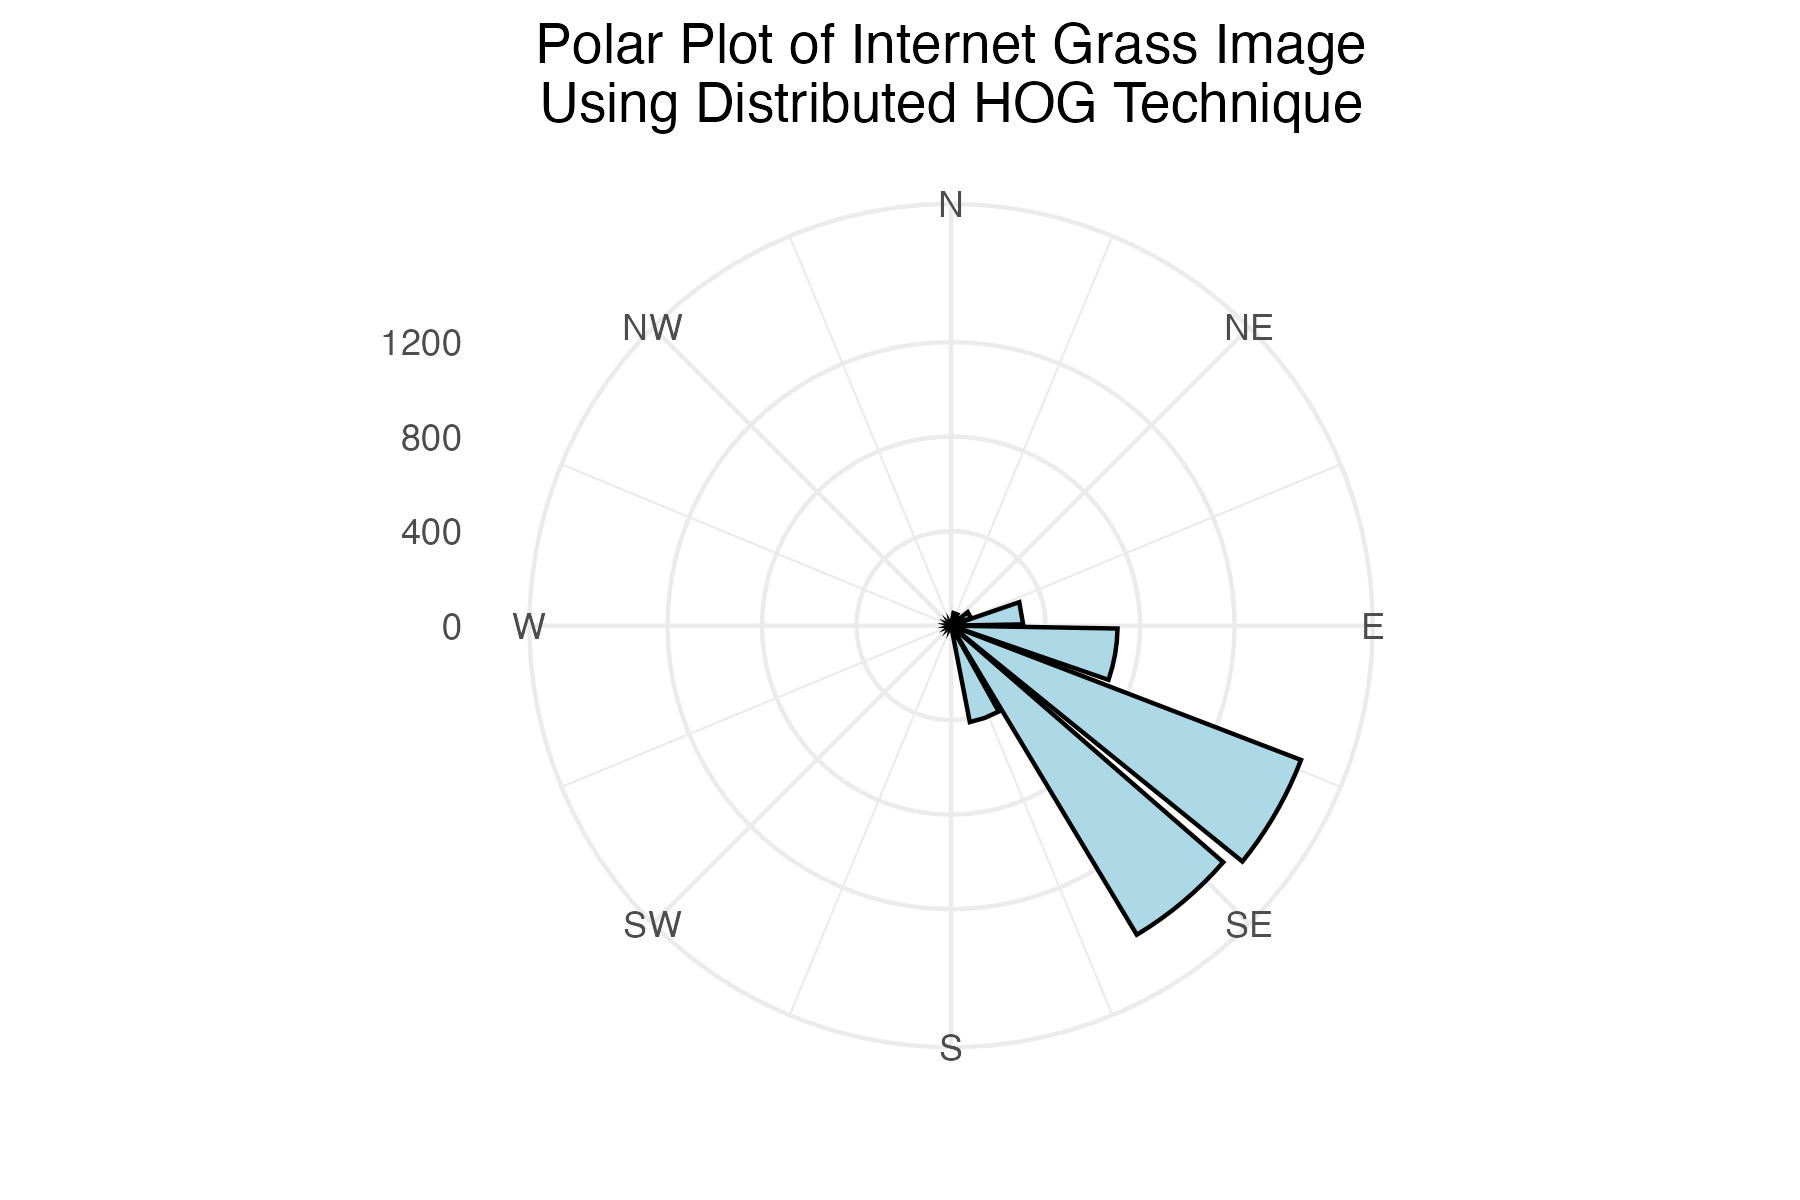
\includegraphics{images/plots/grass/internet_grass_contribution_polar_plot.jpg}

}

\subcaption{Internet Grass Image}

\end{figure}%

\end{minipage}%
%
\begin{minipage}{0.33\linewidth}

\begin{figure}[H]

{\centering 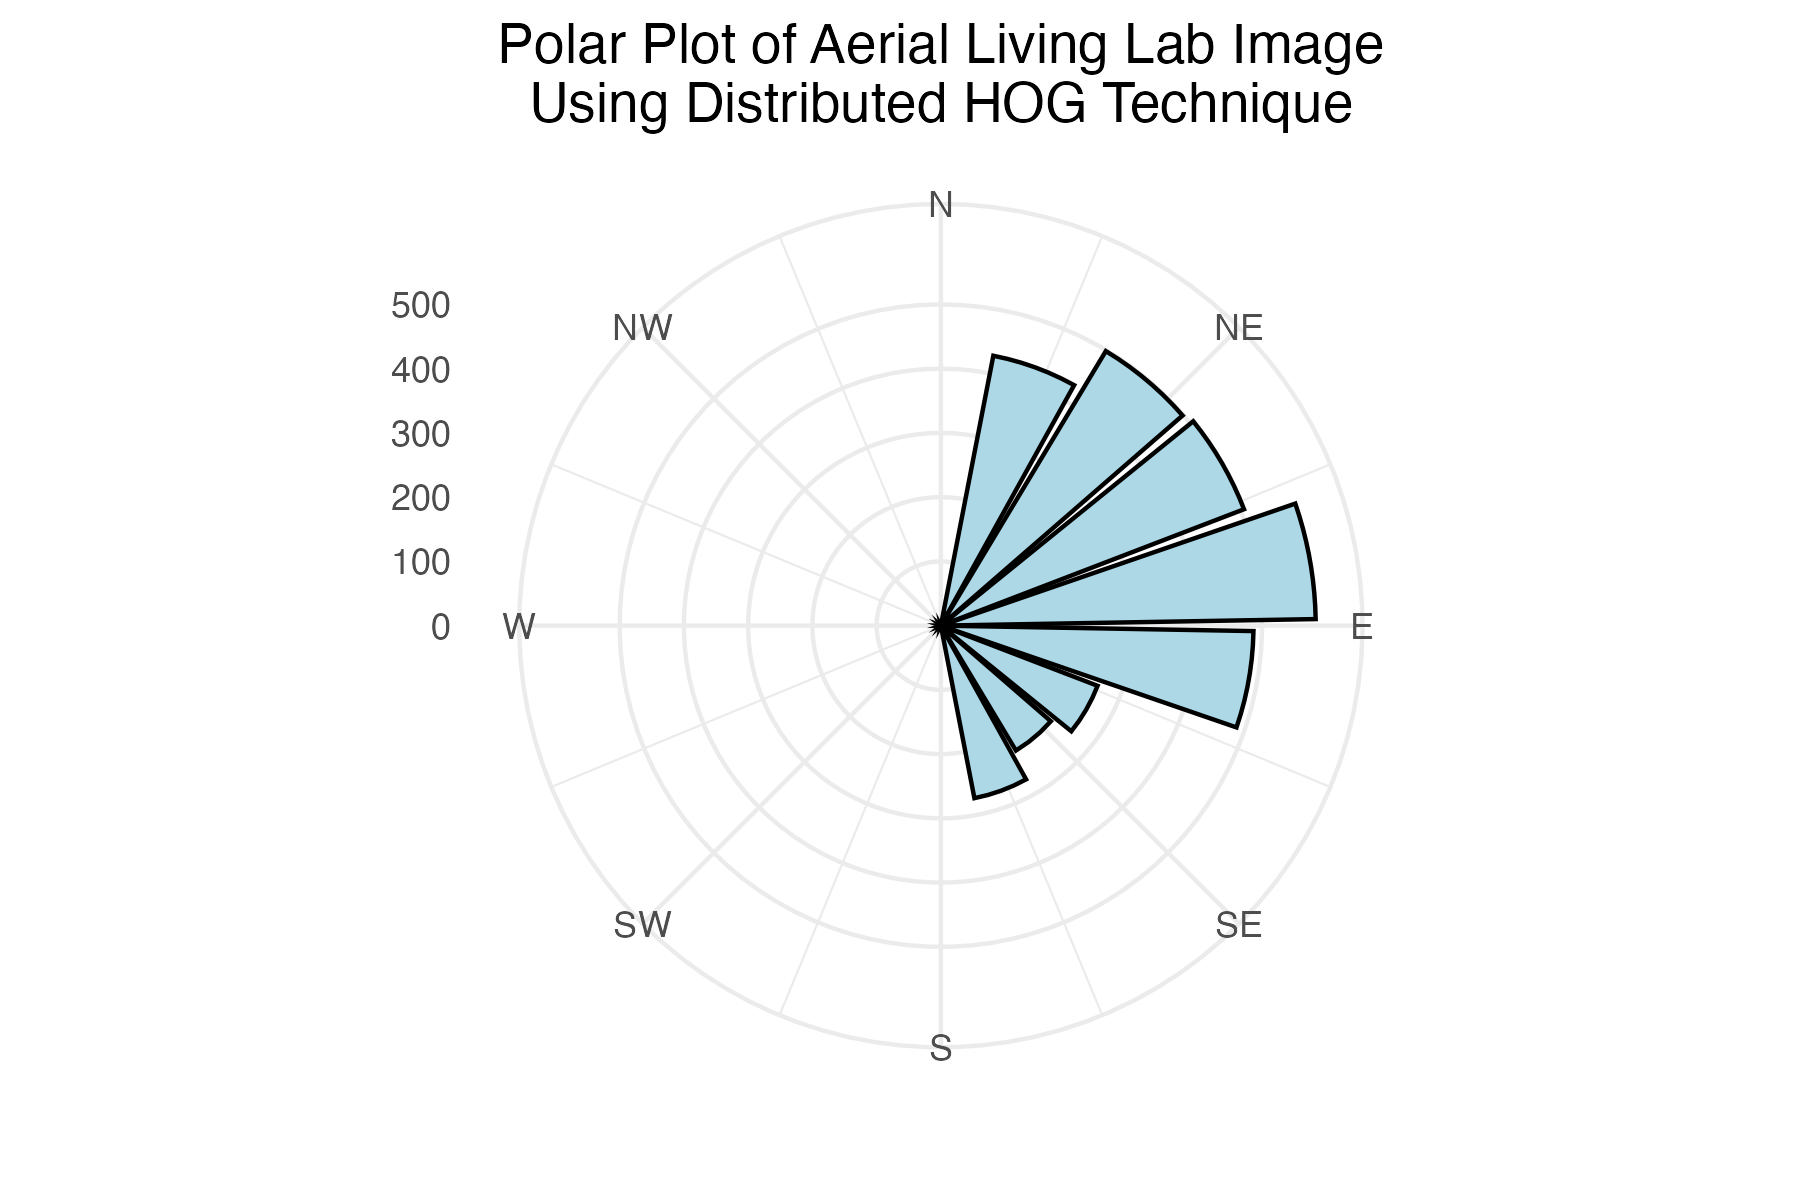
\includegraphics{images/plots/grass/aerial_living_lab_contribution_polar_plot.jpg}

}

\subcaption{Aerial Living Labs Image}

\end{figure}%

\end{minipage}%
%
\begin{minipage}{0.33\linewidth}

\begin{figure}[H]

{\centering 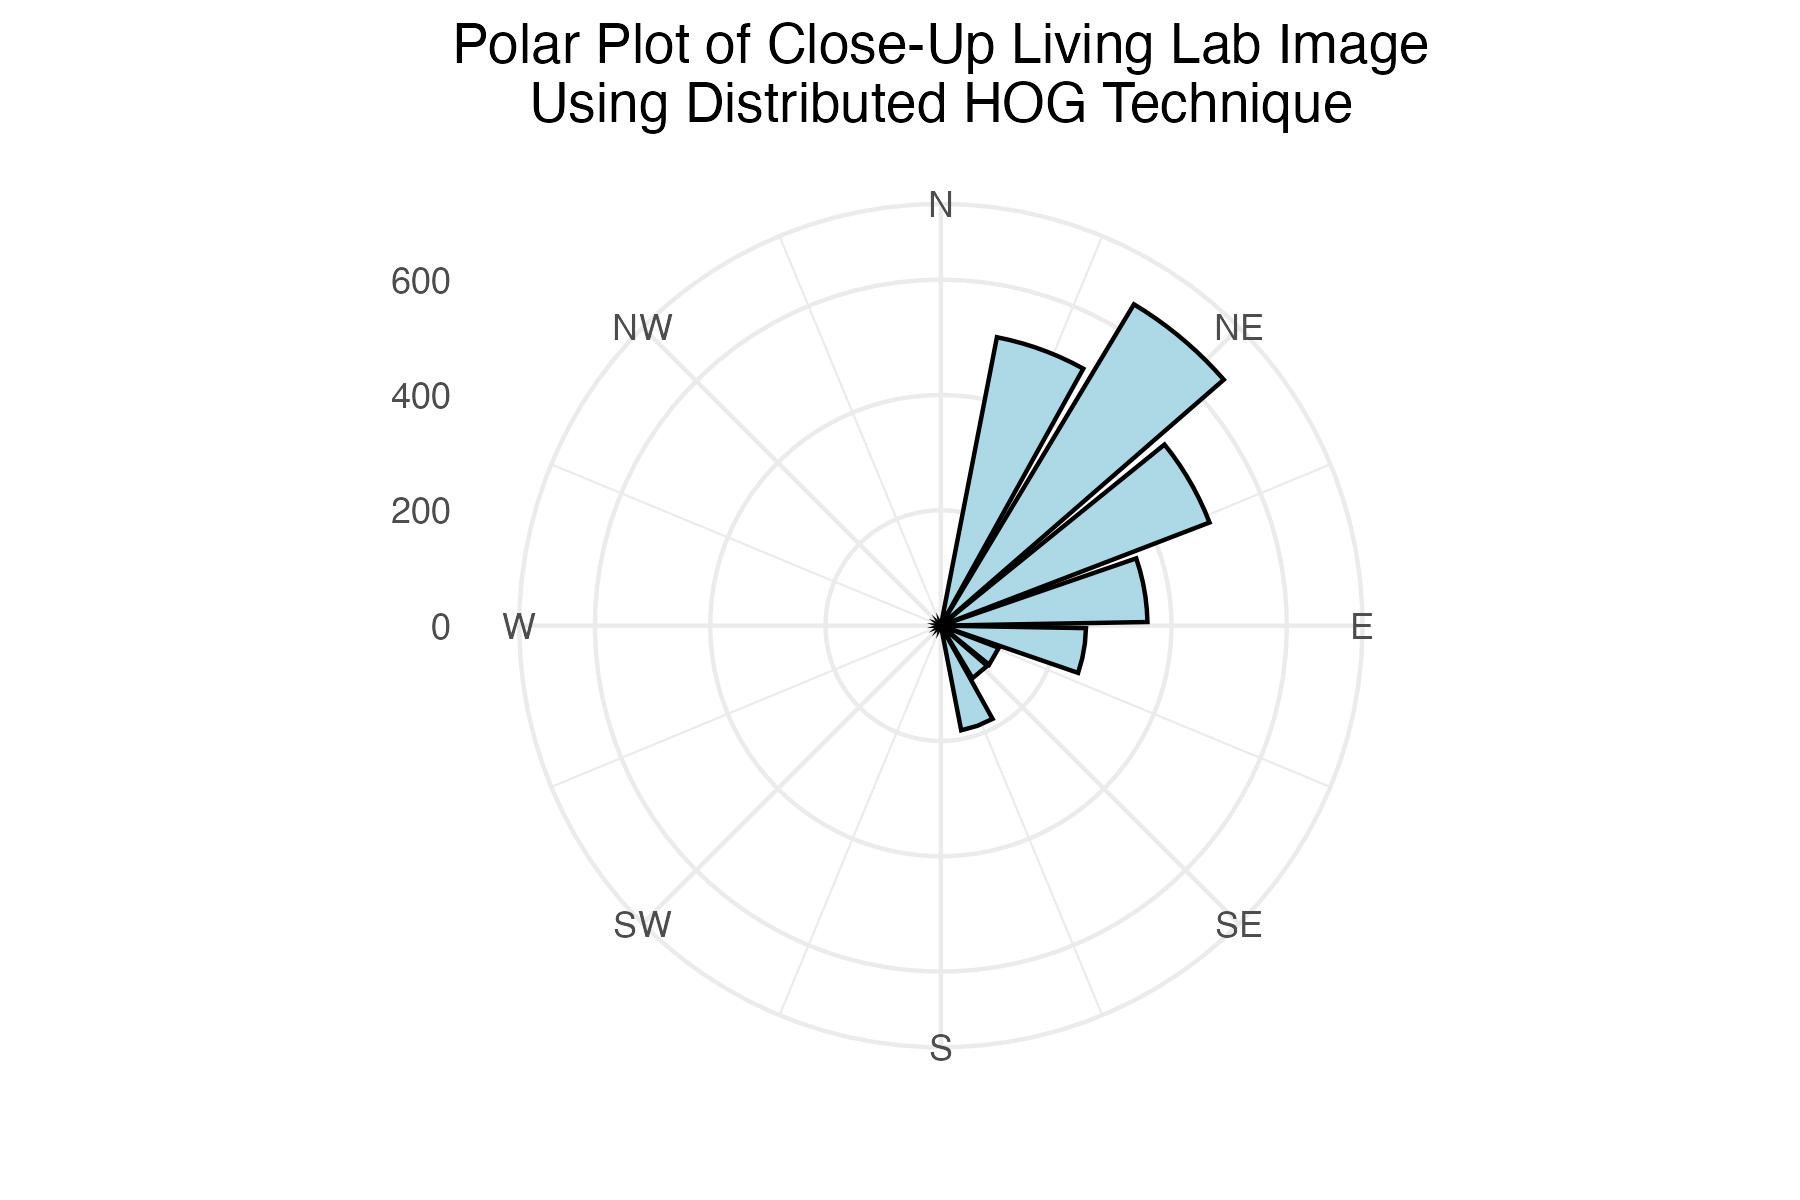
\includegraphics{images/plots/grass/close_up_living_lab_contribution_polar_plot.jpg}

}

\subcaption{Close-Up Living Labs Grass Image}

\end{figure}%

\end{minipage}%

\caption{\label{fig-grass-distributed-polar}Distributed Method Polar
Plots for Grass Images}

\end{figure}%

\chapter{Backflip Image}\label{backflip-image}

\section{Load R Packages and Python
Libraries}\label{load-r-packages-and-python-libraries-2}

\begin{Shaded}
\begin{Highlighting}[]
\CommentTok{\# Load R Packages}
\FunctionTok{library}\NormalTok{(reticulate)}
\FunctionTok{library}\NormalTok{(tidyverse)}
\FunctionTok{library}\NormalTok{(mapsapi)}
\FunctionTok{library}\NormalTok{(mapboxapi)}
\FunctionTok{library}\NormalTok{(magick)}
\end{Highlighting}
\end{Shaded}

\begin{Shaded}
\begin{Highlighting}[]
\CommentTok{\# Load Python Libraries}
\ImportTok{import}\NormalTok{ matplotlib.pyplot }\ImportTok{as}\NormalTok{ plt}
\ImportTok{import}\NormalTok{ pandas }\ImportTok{as}\NormalTok{ pd}
\ImportTok{from}\NormalTok{ skimage.io }\ImportTok{import}\NormalTok{ imread, imshow}
\ImportTok{from}\NormalTok{ skimage.transform }\ImportTok{import}\NormalTok{ resize}
\ImportTok{from}\NormalTok{ skimage.feature }\ImportTok{import}\NormalTok{ hog}
\ImportTok{from}\NormalTok{ skimage }\ImportTok{import}\NormalTok{ data, exposure}
\ImportTok{import}\NormalTok{ matplotlib.pyplot }\ImportTok{as}\NormalTok{ plt}
\ImportTok{from}\NormalTok{ skimage }\ImportTok{import}\NormalTok{ io}
\ImportTok{from}\NormalTok{ skimage }\ImportTok{import}\NormalTok{ color}
\ImportTok{from}\NormalTok{ skimage.transform }\ImportTok{import}\NormalTok{ resize}
\ImportTok{import}\NormalTok{ math}
\ImportTok{from}\NormalTok{ skimage.feature }\ImportTok{import}\NormalTok{ hog}
\ImportTok{import}\NormalTok{ numpy }\ImportTok{as}\NormalTok{ np}
\end{Highlighting}
\end{Shaded}

\section{Collect HOG Features for Backflip
Image}\label{collect-hog-features-for-backflip-image}

\begin{Shaded}
\begin{Highlighting}[]
\CommentTok{\# List for storing images}
\NormalTok{img\_list }\OperatorTok{=}\NormalTok{ []}

\CommentTok{\# SF aerial}
\NormalTok{img\_list.append(color.rgb2gray(io.imread(}\StringTok{"images/TitusFlip.jpg"}\NormalTok{)))}

\CommentTok{\# List to store magnitudes for each image}
\NormalTok{mag\_list }\OperatorTok{=}\NormalTok{ []}

\CommentTok{\# List to store angles for each image}
\NormalTok{theta\_list }\OperatorTok{=}\NormalTok{ []}


\ControlFlowTok{for}\NormalTok{ x }\KeywordTok{in} \BuiltInTok{range}\NormalTok{(}\BuiltInTok{len}\NormalTok{(img\_list)):}
    \CommentTok{\# Get image of interest}
\NormalTok{    img }\OperatorTok{=}\NormalTok{ img\_list[x]}

\NormalTok{    rescaled\_file\_path }\OperatorTok{=} \SpecialStringTok{f"images/plots/backflip/}\SpecialCharTok{\{}\NormalTok{x}\SpecialCharTok{\}}\SpecialStringTok{.jpg"}

    \CommentTok{\# Determine aspect Ratio}
\NormalTok{    aspect\_ratio }\OperatorTok{=}\NormalTok{ img.shape[}\DecValTok{0}\NormalTok{] }\OperatorTok{/}\NormalTok{ img.shape[}\DecValTok{1}\NormalTok{]}
    \BuiltInTok{print}\NormalTok{(}\StringTok{"Aspect Ratio:"}\NormalTok{, aspect\_ratio)}

    \CommentTok{\# Hard{-}Code height to 200 pixels}
\NormalTok{    height }\OperatorTok{=} \DecValTok{200}

    \CommentTok{\# Calculate witdth to maintain same aspect ratio}
\NormalTok{    width }\OperatorTok{=} \BuiltInTok{int}\NormalTok{(height }\OperatorTok{/}\NormalTok{ aspect\_ratio)}
    \BuiltInTok{print}\NormalTok{(}\StringTok{"Resized Width:"}\NormalTok{, width)}

    \CommentTok{\# Resize the image}
\NormalTok{    resized\_img }\OperatorTok{=}\NormalTok{ resize(img, (height, width))}

    \CommentTok{\# Replace the original image with the resized image}
\NormalTok{    img\_list[x] }\OperatorTok{=}\NormalTok{ resized\_img}

    \CommentTok{\# plt.figure(figsize=(15, 8))}
    \CommentTok{\# plt.imshow(resized\_img, cmap="gray")}
    \CommentTok{\# plt.axis("on")}
    \CommentTok{\# plt.tight\_layout()}
    \CommentTok{\# plt.savefig(rescaled\_file\_path, dpi=300)}
    \CommentTok{\# plt.show()}

    \CommentTok{\# list for storing all magnitudes for image[x]}
\NormalTok{    mag }\OperatorTok{=}\NormalTok{ []}

    \CommentTok{\# list for storing all angles for image[x]}
\NormalTok{    theta }\OperatorTok{=}\NormalTok{ []}

    \ControlFlowTok{for}\NormalTok{ i }\KeywordTok{in} \BuiltInTok{range}\NormalTok{(height):}
\NormalTok{        magnitudeArray }\OperatorTok{=}\NormalTok{ []}
\NormalTok{        angleArray }\OperatorTok{=}\NormalTok{ []}

        \ControlFlowTok{for}\NormalTok{ j }\KeywordTok{in} \BuiltInTok{range}\NormalTok{(width):}
            \ControlFlowTok{if}\NormalTok{ j }\OperatorTok{{-}} \DecValTok{1} \OperatorTok{\textless{}} \DecValTok{0} \KeywordTok{or}\NormalTok{ j }\OperatorTok{+} \DecValTok{1} \OperatorTok{\textgreater{}=}\NormalTok{ width:}
                \ControlFlowTok{if}\NormalTok{ j }\OperatorTok{{-}} \DecValTok{1} \OperatorTok{\textless{}} \DecValTok{0}\NormalTok{:}
\NormalTok{                    Gx }\OperatorTok{=}\NormalTok{ resized\_img[i][j }\OperatorTok{+} \DecValTok{1}\NormalTok{] }\OperatorTok{{-}} \DecValTok{0}
                \ControlFlowTok{elif}\NormalTok{ j }\OperatorTok{+} \DecValTok{1} \OperatorTok{\textgreater{}=}\NormalTok{ width:}
\NormalTok{                    Gx }\OperatorTok{=} \DecValTok{0} \OperatorTok{{-}}\NormalTok{ resized\_img[i][j }\OperatorTok{{-}} \DecValTok{1}\NormalTok{]}
            \ControlFlowTok{else}\NormalTok{:}
\NormalTok{                Gx }\OperatorTok{=}\NormalTok{ resized\_img[i][j }\OperatorTok{+} \DecValTok{1}\NormalTok{] }\OperatorTok{{-}}\NormalTok{ resized\_img[i][j }\OperatorTok{{-}} \DecValTok{1}\NormalTok{]}

            \ControlFlowTok{if}\NormalTok{ i }\OperatorTok{{-}} \DecValTok{1} \OperatorTok{\textless{}} \DecValTok{0} \KeywordTok{or}\NormalTok{ i }\OperatorTok{+} \DecValTok{1} \OperatorTok{\textgreater{}=}\NormalTok{ height:}
                \ControlFlowTok{if}\NormalTok{ i }\OperatorTok{{-}} \DecValTok{1} \OperatorTok{\textless{}} \DecValTok{0}\NormalTok{:}
\NormalTok{                    Gy }\OperatorTok{=} \DecValTok{0} \OperatorTok{{-}}\NormalTok{ resized\_img[i }\OperatorTok{+} \DecValTok{1}\NormalTok{][j]}
                \ControlFlowTok{elif}\NormalTok{ i }\OperatorTok{+} \DecValTok{1} \OperatorTok{\textgreater{}=}\NormalTok{ height:}
\NormalTok{                    Gy }\OperatorTok{=}\NormalTok{ resized\_img[i }\OperatorTok{{-}} \DecValTok{1}\NormalTok{][j] }\OperatorTok{{-}} \DecValTok{0}
            \ControlFlowTok{else}\NormalTok{:}
\NormalTok{                Gy }\OperatorTok{=}\NormalTok{ resized\_img[i }\OperatorTok{+} \DecValTok{1}\NormalTok{][j] }\OperatorTok{{-}}\NormalTok{ resized\_img[i }\OperatorTok{{-}} \DecValTok{1}\NormalTok{][j]}

\NormalTok{            magnitude }\OperatorTok{=}\NormalTok{ math.sqrt(}\BuiltInTok{pow}\NormalTok{(Gx, }\DecValTok{2}\NormalTok{) }\OperatorTok{+} \BuiltInTok{pow}\NormalTok{(Gy, }\DecValTok{2}\NormalTok{))}
\NormalTok{            magnitudeArray.append(}\BuiltInTok{round}\NormalTok{(magnitude, }\DecValTok{9}\NormalTok{))}

            \ControlFlowTok{if}\NormalTok{ Gx }\OperatorTok{==} \DecValTok{0}\NormalTok{:}
\NormalTok{                angle }\OperatorTok{=}\NormalTok{ math.degrees(}\FloatTok{0.0}\NormalTok{)}
            \ControlFlowTok{else}\NormalTok{:}
\NormalTok{                angle }\OperatorTok{=}\NormalTok{ math.degrees(math.atan(Gy }\OperatorTok{/}\NormalTok{ Gx))}
                \ControlFlowTok{if}\NormalTok{ angle }\OperatorTok{\textless{}} \DecValTok{0}\NormalTok{:}
\NormalTok{                    angle }\OperatorTok{+=} \DecValTok{180}

\NormalTok{            angleArray.append(}\BuiltInTok{round}\NormalTok{(angle, }\DecValTok{9}\NormalTok{))}

\NormalTok{        mag.append(magnitudeArray)}
\NormalTok{        theta.append(angleArray)}

    \CommentTok{\# add list of magnitudes to list[x]}
\NormalTok{    mag\_list.append(mag)}

    \CommentTok{\# add list of angles to angle list[x]}
\NormalTok{    theta\_list.append(theta)}
\end{Highlighting}
\end{Shaded}

\begin{verbatim}
Aspect Ratio: 1.25
Resized Width: 160
\end{verbatim}

\begin{figure}

\begin{minipage}{\linewidth}

\begin{figure}[H]

{\centering 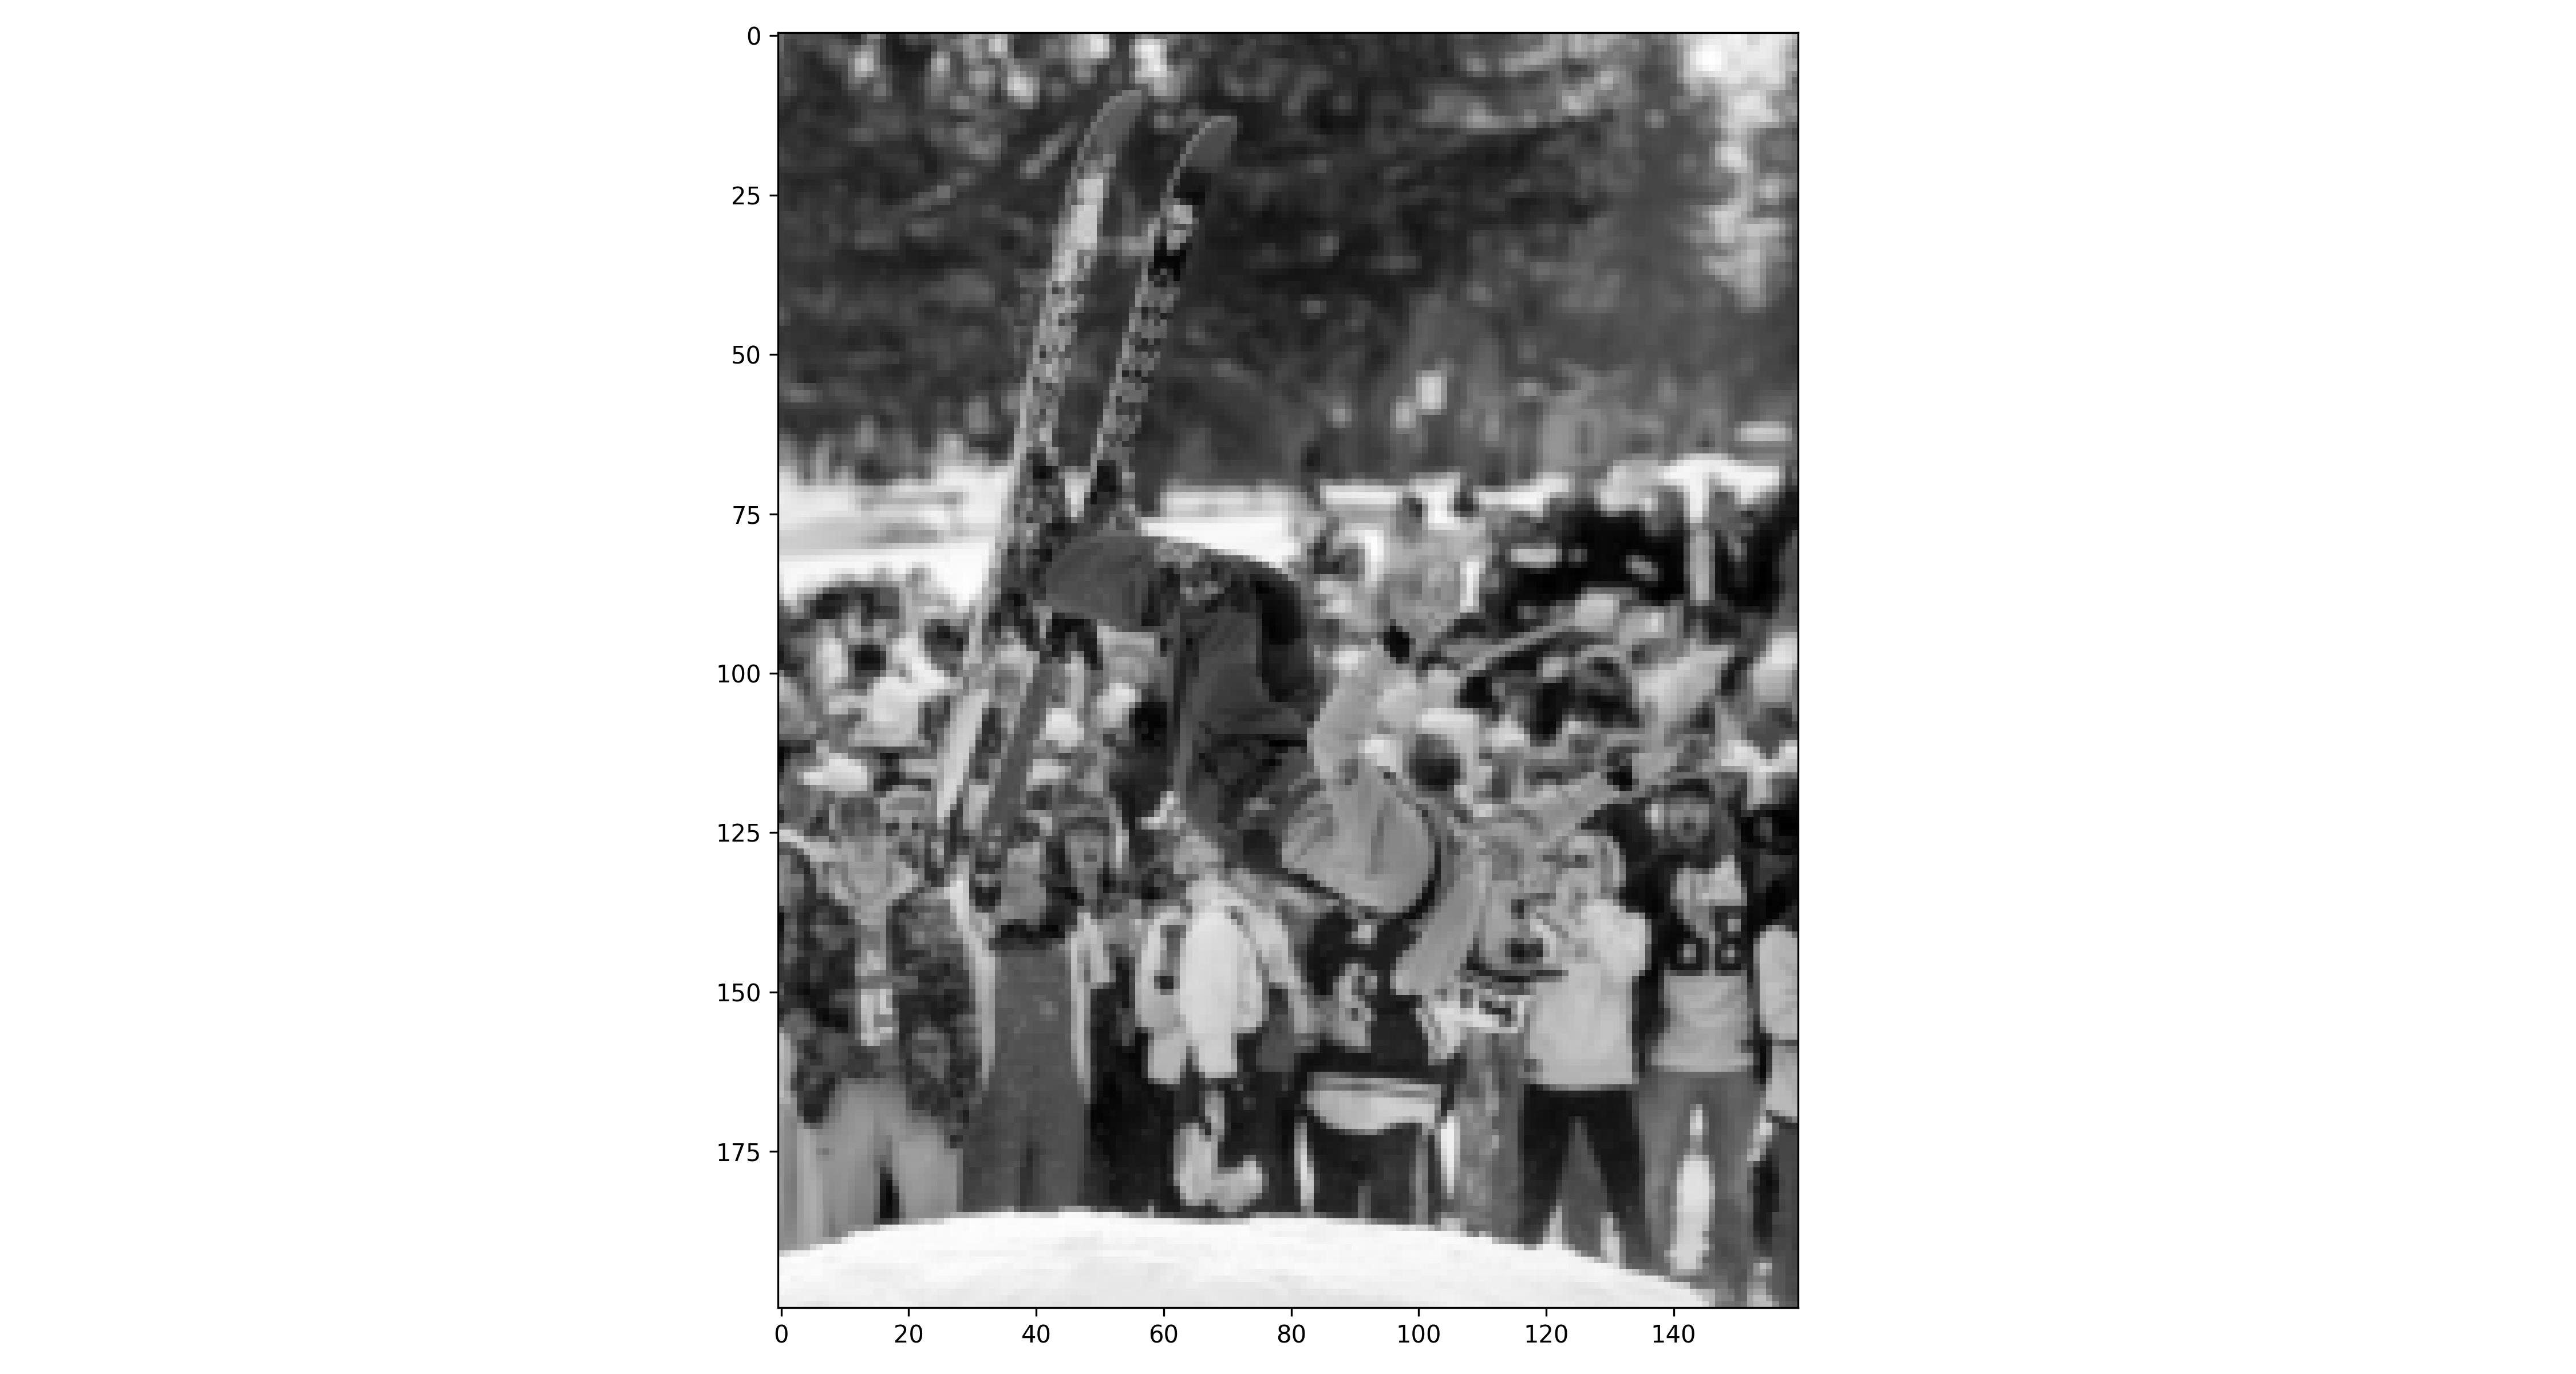
\includegraphics{images/plots/backflip/0.jpg}

}

\subcaption{Skiing Backflip}

\end{figure}%

\end{minipage}%

\caption{\label{fig-flip}Skiing Backflip Image Rescaled and Converted to
Greyscale}

\end{figure}%

\section{Extract Gradient Magnitudes and Angles from Backflip
Image}\label{extract-gradient-magnitudes-and-angles-from-backflip-image}

\begin{Shaded}
\begin{Highlighting}[]
\CommentTok{\# DF of gradient magnitudes and angles}
\NormalTok{mag\_flip }\OperatorTok{=}\NormalTok{ np.array(mag\_list[}\DecValTok{0}\NormalTok{])}
\NormalTok{theta\_flip }\OperatorTok{=}\NormalTok{ np.array(theta\_list[}\DecValTok{0}\NormalTok{])}
\end{Highlighting}
\end{Shaded}

\section{Plot Magnitudes as Image for Backflip
Image}\label{plot-magnitudes-as-image-for-backflip-image}

\begin{Shaded}
\begin{Highlighting}[]
\CommentTok{\# Save gradient magnitudes of backflip in image form}

\CommentTok{\# plt.figure(figsize=(15, 8))}
\CommentTok{\# \#plt.title(\textquotesingle{}San Francisco, CA Gradient Magnitudes\textquotesingle{})}
\CommentTok{\# plt.imshow(mag\_list[0], cmap="gray")}
\CommentTok{\# plt.axis("on")}
\CommentTok{\# \#plt.show()}
\CommentTok{\# plt.tight\_layout()}
\CommentTok{\# plt.savefig("images/plots/backflip/backflip\_mag.png", dpi=300)}
\end{Highlighting}
\end{Shaded}

\begin{figure}

\begin{minipage}{\linewidth}

\begin{figure}[H]

{\centering \includegraphics{images/plots/backflip/backflip_mag.png}

}

\subcaption{Skiing Backflip Image}

\end{figure}%

\end{minipage}%

\caption{\label{fig-backflip-mags}Skiing Backflip Cityscape Magnitudes
as Image}

\end{figure}%

\section{Create Data Frame for Backflip
Image}\label{create-data-frame-for-backflip-image}

\begin{Shaded}
\begin{Highlighting}[]
\CommentTok{\# Flip DF}
\NormalTok{backflip\_hog\_df }\OtherTok{\textless{}{-}} \FunctionTok{data.frame}\NormalTok{(}\AttributeTok{mag =} \FunctionTok{as.vector}\NormalTok{(py}\SpecialCharTok{$}\NormalTok{mag\_flip),}
                              \AttributeTok{theta =} \FunctionTok{as.vector}\NormalTok{((py}\SpecialCharTok{$}\NormalTok{theta\_flip))) }\SpecialCharTok{\%\textgreater{}\%}
  \FunctionTok{mutate}\NormalTok{(}\AttributeTok{radian =}\NormalTok{ theta}\SpecialCharTok{*}\NormalTok{(pi}\SpecialCharTok{/}\DecValTok{180}\NormalTok{))}

\CommentTok{\# Add to list}
\NormalTok{flip\_standard\_df\_list }\OtherTok{=} \FunctionTok{list}\NormalTok{(backflip\_hog\_df)}
\end{Highlighting}
\end{Shaded}

\section{Create Histograms of Gradient Magnitudes and Angles for
Backflip
Image}\label{create-histograms-of-gradient-magnitudes-and-angles-for-backflip-image}

\begin{Shaded}
\begin{Highlighting}[]
\CommentTok{\# backflip histogram of gradient mags}
\NormalTok{flip\_histogram\_mag\_plot }\OtherTok{\textless{}{-}}
  \FunctionTok{ggplot}\NormalTok{(flip\_standard\_df\_list[[}\DecValTok{1}\NormalTok{]],}
         \FunctionTok{aes}\NormalTok{(}\AttributeTok{x =}\NormalTok{ mag)) }\SpecialCharTok{+}
  \FunctionTok{geom\_histogram}\NormalTok{(}\AttributeTok{colour =} \StringTok{"black"}\NormalTok{, }\AttributeTok{fill =} \StringTok{"lightblue"}\NormalTok{) }\SpecialCharTok{+}
  \FunctionTok{scale\_x\_continuous}\NormalTok{() }\SpecialCharTok{+}
  \FunctionTok{labs}\NormalTok{(}\AttributeTok{x =} \StringTok{"Gradient Magnitude"}\NormalTok{,}
       \AttributeTok{y =} \StringTok{"Count"}\NormalTok{,}
       \AttributeTok{title =} \StringTok{"Skiing Backflip Image Histogram of Gradient Magnitudes"}
\NormalTok{       ) }\SpecialCharTok{+}
  \FunctionTok{theme\_minimal}\NormalTok{() }\SpecialCharTok{+}
  \FunctionTok{theme}\NormalTok{(}\AttributeTok{plot.title =} \FunctionTok{element\_text}\NormalTok{(}\AttributeTok{hjust =} \FloatTok{0.5}\NormalTok{))}

\CommentTok{\# flip magn filter level}
\NormalTok{flip\_mag\_filter }\OtherTok{\textless{}{-}} \FloatTok{0.2}

\CommentTok{\# save image}
\FunctionTok{ggsave}\NormalTok{(}\StringTok{"images/plots/backflip/backflip\_histogram\_mag\_plot.jpg"}\NormalTok{, flip\_histogram\_mag\_plot, }\AttributeTok{width =} \DecValTok{6}\NormalTok{, }\AttributeTok{height =} \DecValTok{4}\NormalTok{, }\AttributeTok{dpi =} \DecValTok{300}\NormalTok{)}
\end{Highlighting}
\end{Shaded}

\begin{Shaded}
\begin{Highlighting}[]
\CommentTok{\# backflip histogram of gradient angles}
\NormalTok{flip\_histogram\_theta\_plot }\OtherTok{\textless{}{-}}
  \FunctionTok{ggplot}\NormalTok{(flip\_standard\_df\_list[[}\DecValTok{1}\NormalTok{]],}
         \FunctionTok{aes}\NormalTok{(}\AttributeTok{x =}\NormalTok{ theta)) }\SpecialCharTok{+}
  \FunctionTok{geom\_histogram}\NormalTok{(}\AttributeTok{colour =} \StringTok{"black"}\NormalTok{, }\AttributeTok{fill =} \StringTok{"lightblue"}\NormalTok{) }\SpecialCharTok{+}
  \FunctionTok{scale\_x\_continuous}\NormalTok{() }\SpecialCharTok{+}
  \FunctionTok{labs}\NormalTok{(}\AttributeTok{x =} \StringTok{"Gradient Angle"}\NormalTok{,}
       \AttributeTok{y =} \StringTok{"Count"}\NormalTok{,}
       \AttributeTok{title =} \StringTok{"Skiing Backflip Image Histogram of Gradient Angles"}
\NormalTok{       ) }\SpecialCharTok{+}
  \FunctionTok{theme\_minimal}\NormalTok{() }\SpecialCharTok{+}
  \FunctionTok{theme}\NormalTok{(}\AttributeTok{plot.title =} \FunctionTok{element\_text}\NormalTok{(}\AttributeTok{hjust =} \FloatTok{0.5}\NormalTok{))}

\CommentTok{\# save image}
\FunctionTok{ggsave}\NormalTok{(}\StringTok{"images/plots/backflip/backflip\_histogram\_theta\_plot.jpg"}\NormalTok{, flip\_histogram\_theta\_plot, }\AttributeTok{width =} \DecValTok{6}\NormalTok{, }\AttributeTok{height =} \DecValTok{4}\NormalTok{, }\AttributeTok{dpi =} \DecValTok{300}\NormalTok{)}
\end{Highlighting}
\end{Shaded}

\begin{figure}

\begin{minipage}{0.50\linewidth}

\begin{figure}[H]

{\centering \includegraphics{images/plots/backflip/backflip_histogram_mag_plot.jpg}

}

\subcaption{Skiing Backflip Histogram of Gradient Magnitudes}

\end{figure}%

\end{minipage}%
%
\begin{minipage}{0.50\linewidth}

\begin{figure}[H]

{\centering \includegraphics{images/plots/backflip/backflip_histogram_theta_plot.jpg}

}

\subcaption{Skiing Backflip Histogram of Gradient Angles}

\end{figure}%

\end{minipage}%

\caption{\label{fig-flip-histograms}Skiing Backflip Magnitudes and
Angles}

\end{figure}%

\section{Build New Distributed Histogram Data Frame for Backflip
Image}\label{build-new-distributed-histogram-data-frame-for-backflip-image}

\begin{Shaded}
\begin{Highlighting}[]
\CommentTok{\# function to calculate the contributions to neighboring bins}
\NormalTok{calculate\_bin\_contributions }\OtherTok{\textless{}{-}} \ControlFlowTok{function}\NormalTok{(angle, magnitude, num\_bins) \{}
\NormalTok{  bin\_width }\OtherTok{\textless{}{-}} \DecValTok{180} \SpecialCharTok{/}\NormalTok{ num\_bins}
\NormalTok{  contributions }\OtherTok{\textless{}{-}} \FunctionTok{numeric}\NormalTok{(num\_bins)}
  
  \CommentTok{\# get the central bin}
\NormalTok{  central\_bin }\OtherTok{\textless{}{-}} \FunctionTok{floor}\NormalTok{(angle }\SpecialCharTok{/}\NormalTok{ bin\_width) }\SpecialCharTok{\%\%}\NormalTok{ num\_bins}
\NormalTok{  next\_bin }\OtherTok{\textless{}{-}}\NormalTok{ (central\_bin }\SpecialCharTok{+} \DecValTok{1}\NormalTok{) }\SpecialCharTok{\%\%}\NormalTok{ num\_bins}
  
  \CommentTok{\# get contributions to neighboring bins}
\NormalTok{  weight }\OtherTok{\textless{}{-}}\NormalTok{ (}\DecValTok{1} \SpecialCharTok{{-}} \FunctionTok{abs}\NormalTok{((angle }\SpecialCharTok{\%\%}\NormalTok{ bin\_width) }\SpecialCharTok{/}\NormalTok{ bin\_width)) }\SpecialCharTok{*}\NormalTok{ magnitude}
  
\NormalTok{  contributions[central\_bin }\SpecialCharTok{+} \DecValTok{1}\NormalTok{] }\OtherTok{\textless{}{-}}\NormalTok{ weight}
\NormalTok{  contributions[next\_bin }\SpecialCharTok{+} \DecValTok{1}\NormalTok{] }\OtherTok{\textless{}{-}}\NormalTok{ magnitude }\SpecialCharTok{{-}}\NormalTok{ weight}
  
  \FunctionTok{return}\NormalTok{(}\FunctionTok{list}\NormalTok{(contributions[}\DecValTok{1}\NormalTok{],}
\NormalTok{         contributions[}\DecValTok{2}\NormalTok{],}
\NormalTok{         contributions[}\DecValTok{3}\NormalTok{],}
\NormalTok{         contributions[}\DecValTok{4}\NormalTok{],}
\NormalTok{         contributions[}\DecValTok{5}\NormalTok{],}
\NormalTok{         contributions[}\DecValTok{6}\NormalTok{],}
\NormalTok{         contributions[}\DecValTok{7}\NormalTok{],}
\NormalTok{         contributions[}\DecValTok{8}\NormalTok{],}
\NormalTok{         contributions[}\DecValTok{9}\NormalTok{])}
\NormalTok{         )}
\NormalTok{\}}
\end{Highlighting}
\end{Shaded}

\begin{Shaded}
\begin{Highlighting}[]
\CommentTok{\# Create filtered data frames using the filter level for magnitudes defined above, store in a list}
\NormalTok{filtered\_flip\_standard\_df\_list }\OtherTok{\textless{}{-}}\FunctionTok{list}\NormalTok{(backflip\_hog\_df }\SpecialCharTok{\%\textgreater{}\%}
                                        \FunctionTok{filter}\NormalTok{(mag }\SpecialCharTok{\textgreater{}=}\NormalTok{ flip\_mag\_filter))}
\end{Highlighting}
\end{Shaded}

\begin{Shaded}
\begin{Highlighting}[]
\CommentTok{\# Define the number of bins}
\NormalTok{num\_bins }\OtherTok{\textless{}{-}} \DecValTok{9}
\NormalTok{flip\_contribution\_df\_list }\OtherTok{\textless{}{-}} \FunctionTok{list}\NormalTok{()}

\CommentTok{\# iterate through each filtered standard data frame (only 1 in this case)}
\ControlFlowTok{for}\NormalTok{ (i }\ControlFlowTok{in} \DecValTok{1}\SpecialCharTok{:}\FunctionTok{length}\NormalTok{(filtered\_flip\_standard\_df\_list))\{}

\NormalTok{  flip\_contribution\_hog\_df }\OtherTok{\textless{}{-}}
\NormalTok{    filtered\_flip\_standard\_df\_list[[i]] }\SpecialCharTok{\%\textgreater{}\%}
    \FunctionTok{rowwise}\NormalTok{() }\SpecialCharTok{\%\textgreater{}\%}
    \FunctionTok{mutate}\NormalTok{(}\StringTok{\textasciigrave{}}\AttributeTok{0}\StringTok{\textasciigrave{}} \OtherTok{=} \FunctionTok{calculate\_bin\_contributions}\NormalTok{(theta, mag, }\DecValTok{9}\NormalTok{)[[}\DecValTok{1}\NormalTok{]],}
           \StringTok{\textasciigrave{}}\AttributeTok{20}\StringTok{\textasciigrave{}} \OtherTok{=} \FunctionTok{calculate\_bin\_contributions}\NormalTok{(theta, mag, }\DecValTok{9}\NormalTok{)[[}\DecValTok{2}\NormalTok{]],}
           \StringTok{\textasciigrave{}}\AttributeTok{40}\StringTok{\textasciigrave{}} \OtherTok{=} \FunctionTok{calculate\_bin\_contributions}\NormalTok{(theta, mag, }\DecValTok{9}\NormalTok{)[[}\DecValTok{3}\NormalTok{]],}
           \StringTok{\textasciigrave{}}\AttributeTok{60}\StringTok{\textasciigrave{}} \OtherTok{=} \FunctionTok{calculate\_bin\_contributions}\NormalTok{(theta, mag, }\DecValTok{9}\NormalTok{)[[}\DecValTok{4}\NormalTok{]],}
           \StringTok{\textasciigrave{}}\AttributeTok{80}\StringTok{\textasciigrave{}} \OtherTok{=} \FunctionTok{calculate\_bin\_contributions}\NormalTok{(theta, mag, }\DecValTok{9}\NormalTok{)[[}\DecValTok{5}\NormalTok{]],}
           \StringTok{\textasciigrave{}}\AttributeTok{100}\StringTok{\textasciigrave{}} \OtherTok{=} \FunctionTok{calculate\_bin\_contributions}\NormalTok{(theta, mag, }\DecValTok{9}\NormalTok{)[[}\DecValTok{6}\NormalTok{]],}
           \StringTok{\textasciigrave{}}\AttributeTok{120}\StringTok{\textasciigrave{}} \OtherTok{=} \FunctionTok{calculate\_bin\_contributions}\NormalTok{(theta, mag, }\DecValTok{9}\NormalTok{)[[}\DecValTok{7}\NormalTok{]],}
           \StringTok{\textasciigrave{}}\AttributeTok{140}\StringTok{\textasciigrave{}} \OtherTok{=} \FunctionTok{calculate\_bin\_contributions}\NormalTok{(theta, mag, }\DecValTok{9}\NormalTok{)[[}\DecValTok{8}\NormalTok{]],}
           \StringTok{\textasciigrave{}}\AttributeTok{160}\StringTok{\textasciigrave{}} \OtherTok{=} \FunctionTok{calculate\_bin\_contributions}\NormalTok{(theta, mag, }\DecValTok{9}\NormalTok{)[[}\DecValTok{9}\NormalTok{]],}
\NormalTok{           )}
  
  \CommentTok{\# rearrange into same tidy format}
\NormalTok{  flip\_split\_histo\_df }\OtherTok{\textless{}{-}}
\NormalTok{    flip\_contribution\_hog\_df }\SpecialCharTok{\%\textgreater{}\%}
    \FunctionTok{pivot\_longer}\NormalTok{(}\AttributeTok{names\_to =} \StringTok{"bin"}\NormalTok{,}
                 \AttributeTok{values\_to =} \StringTok{"contribution"}\NormalTok{,}
                 \AttributeTok{cols =} \DecValTok{4}\SpecialCharTok{:}\FunctionTok{ncol}\NormalTok{(flip\_contribution\_hog\_df)) }\SpecialCharTok{\%\textgreater{}\%}
    \FunctionTok{mutate}\NormalTok{(}\AttributeTok{bin =} \FunctionTok{as.numeric}\NormalTok{(bin)) }\SpecialCharTok{\%\textgreater{}\%}
    \FunctionTok{group\_by}\NormalTok{(bin) }\SpecialCharTok{\%\textgreater{}\%}
    \FunctionTok{summarise}\NormalTok{(}\AttributeTok{contribution\_sum =} \FunctionTok{sum}\NormalTok{(contribution))}

  \CommentTok{\# add to list for storage}
\NormalTok{  flip\_contribution\_df\_list[[i]] }\OtherTok{\textless{}{-}}\NormalTok{ flip\_split\_histo\_df}

\NormalTok{\}}
\end{Highlighting}
\end{Shaded}

\section{Generate Polar Plots for Standard Historgrams for Backflip
Image}\label{generate-polar-plots-for-standard-historgrams-for-backflip-image}

\begin{Shaded}
\begin{Highlighting}[]
\CommentTok{\# backflip plot}
\NormalTok{flip\_plot }\OtherTok{\textless{}{-}}
  \FunctionTok{ggplot}\NormalTok{(filtered\_flip\_standard\_df\_list[[}\DecValTok{1}\NormalTok{]],}
         \FunctionTok{aes}\NormalTok{(}\AttributeTok{x =}\NormalTok{ theta)) }\SpecialCharTok{+}
  \FunctionTok{geom\_histogram}\NormalTok{(}\AttributeTok{colour =} \StringTok{"black"}\NormalTok{,}
                 \AttributeTok{fill =} \StringTok{"lightblue"}\NormalTok{,}
                 \AttributeTok{breaks =} \FunctionTok{seq}\NormalTok{(}\DecValTok{0}\NormalTok{, }\DecValTok{360}\NormalTok{, }\AttributeTok{length.out =} \FloatTok{17.5}\NormalTok{),}
                 \AttributeTok{bins =} \DecValTok{9}\NormalTok{) }\SpecialCharTok{+}
  \FunctionTok{coord\_polar}\NormalTok{(}
    \AttributeTok{theta =} \StringTok{"x"}\NormalTok{,}
    \AttributeTok{start =} \DecValTok{0}\NormalTok{,}
    \AttributeTok{direction =} \DecValTok{1}\NormalTok{) }\SpecialCharTok{+}
  \FunctionTok{scale\_x\_continuous}\NormalTok{(}\AttributeTok{limits =} \FunctionTok{c}\NormalTok{(}\DecValTok{0}\NormalTok{,}\DecValTok{360}\NormalTok{),}
    \AttributeTok{breaks =} \FunctionTok{c}\NormalTok{(}\DecValTok{0}\NormalTok{, }\DecValTok{45}\NormalTok{, }\DecValTok{90}\NormalTok{, }\DecValTok{135}\NormalTok{, }\DecValTok{180}\NormalTok{, }\DecValTok{225}\NormalTok{, }\DecValTok{270}\NormalTok{, }\DecValTok{315}\NormalTok{),}
    \AttributeTok{labels =} \FunctionTok{c}\NormalTok{(}\StringTok{"N"}\NormalTok{, }\StringTok{"NE"}\NormalTok{, }\StringTok{"E"}\NormalTok{, }\StringTok{"SE"}\NormalTok{, }\StringTok{"S"}\NormalTok{, }\StringTok{"SW"}\NormalTok{, }\StringTok{"W"}\NormalTok{, }\StringTok{"NW"}\NormalTok{)}
\NormalTok{  )}\SpecialCharTok{+}
  \FunctionTok{labs}\NormalTok{(}\AttributeTok{title =} \StringTok{"Polar Plot of Skiing Backflip Image}\SpecialCharTok{\textbackslash{}n}\StringTok{Using Standard HOG Technique"}\NormalTok{) }\SpecialCharTok{+}
  \FunctionTok{theme\_minimal}\NormalTok{() }\SpecialCharTok{+}
  \FunctionTok{labs}\NormalTok{(}\AttributeTok{x =} \StringTok{""}\NormalTok{) }\SpecialCharTok{+}
  \FunctionTok{theme}\NormalTok{(}\AttributeTok{axis.title.y =} \FunctionTok{element\_blank}\NormalTok{(),}
        \AttributeTok{plot.title =} \FunctionTok{element\_text}\NormalTok{(}\AttributeTok{hjust =} \FloatTok{0.5}\NormalTok{))}

\CommentTok{\# save image}
\FunctionTok{ggsave}\NormalTok{(}\StringTok{"images/plots/backflip/backflip\_standard\_polar\_plot.jpg"}\NormalTok{, flip\_plot, }\AttributeTok{width =} \DecValTok{6}\NormalTok{, }\AttributeTok{height =} \DecValTok{4}\NormalTok{, }\AttributeTok{dpi =} \DecValTok{300}\NormalTok{)}
\end{Highlighting}
\end{Shaded}

\section{Generate Polar Plots for Distributed Historgrams of Diagonal
Image}\label{generate-polar-plots-for-distributed-historgrams-of-diagonal-image}

\begin{Shaded}
\begin{Highlighting}[]
\CommentTok{\# backflip plot}
\NormalTok{flip\_split\_plot }\OtherTok{\textless{}{-}}
  \FunctionTok{ggplot}\NormalTok{(flip\_contribution\_df\_list[[}\DecValTok{1}\NormalTok{]],}
         \FunctionTok{aes}\NormalTok{(}\AttributeTok{x =}\NormalTok{ bin, }\AttributeTok{y =}\NormalTok{ contribution\_sum)) }\SpecialCharTok{+}
  \FunctionTok{geom\_histogram}\NormalTok{(}\AttributeTok{stat =} \StringTok{"identity"}\NormalTok{,}
                 \AttributeTok{colour =} \StringTok{"black"}\NormalTok{,}
                 \AttributeTok{fill =} \StringTok{"lightblue"}\NormalTok{,}
                 \AttributeTok{breaks =} \FunctionTok{seq}\NormalTok{(}\DecValTok{0}\NormalTok{, }\DecValTok{360}\NormalTok{, }\AttributeTok{length.out =} \FloatTok{17.5}\NormalTok{),}
                 \AttributeTok{bins =} \DecValTok{9}\NormalTok{) }\SpecialCharTok{+}
  \FunctionTok{coord\_polar}\NormalTok{(}
    \AttributeTok{theta =} \StringTok{"x"}\NormalTok{,}
    \AttributeTok{start =} \DecValTok{0}\NormalTok{,}
    \AttributeTok{direction =} \DecValTok{1}\NormalTok{) }\SpecialCharTok{+}
  \FunctionTok{scale\_x\_continuous}\NormalTok{(}\AttributeTok{limits =} \FunctionTok{c}\NormalTok{(}\DecValTok{0}\NormalTok{,}\DecValTok{360}\NormalTok{),}
    \AttributeTok{breaks =} \FunctionTok{c}\NormalTok{(}\DecValTok{0}\NormalTok{, }\DecValTok{45}\NormalTok{, }\DecValTok{90}\NormalTok{, }\DecValTok{135}\NormalTok{, }\DecValTok{180}\NormalTok{, }\DecValTok{225}\NormalTok{, }\DecValTok{270}\NormalTok{, }\DecValTok{315}\NormalTok{),}
    \AttributeTok{labels =} \FunctionTok{c}\NormalTok{(}\StringTok{"N"}\NormalTok{, }\StringTok{"NE"}\NormalTok{, }\StringTok{"E"}\NormalTok{, }\StringTok{"SE"}\NormalTok{, }\StringTok{"S"}\NormalTok{, }\StringTok{"SW"}\NormalTok{, }\StringTok{"W"}\NormalTok{, }\StringTok{"NW"}\NormalTok{)}
\NormalTok{  )}\SpecialCharTok{+}
  \FunctionTok{labs}\NormalTok{(}\AttributeTok{title =} \StringTok{"Polar Plot of Skiing Backflip Image}\SpecialCharTok{\textbackslash{}n}\StringTok{Using Distributed HOG Technique"}\NormalTok{) }\SpecialCharTok{+}
  \FunctionTok{theme\_minimal}\NormalTok{() }\SpecialCharTok{+}
  \FunctionTok{labs}\NormalTok{(}\AttributeTok{x =} \StringTok{""}\NormalTok{) }\SpecialCharTok{+}
  \FunctionTok{theme}\NormalTok{(}\AttributeTok{axis.title.y =} \FunctionTok{element\_blank}\NormalTok{(),}
        \AttributeTok{plot.title =} \FunctionTok{element\_text}\NormalTok{(}\AttributeTok{hjust =} \FloatTok{0.5}\NormalTok{))}

\CommentTok{\# save image}
\FunctionTok{ggsave}\NormalTok{(}\StringTok{"images/plots/backflip/backflip\_contribution\_polar\_plot.jpg"}\NormalTok{, flip\_split\_plot, }\AttributeTok{width =} \DecValTok{6}\NormalTok{, }\AttributeTok{height =} \DecValTok{4}\NormalTok{, }\AttributeTok{dpi =} \DecValTok{300}\NormalTok{)}
\end{Highlighting}
\end{Shaded}

\begin{figure}

\begin{minipage}{0.50\linewidth}

\begin{figure}[H]

{\centering \includegraphics{images/plots/backflip/backflip_standard_polar_plot.jpg}

}

\subcaption{Skiing Backflip Image Standard HOG Method}

\end{figure}%

\end{minipage}%
%
\begin{minipage}{0.50\linewidth}

\begin{figure}[H]

{\centering \includegraphics{images/plots/backflip/backflip_contribution_polar_plot.jpg}

}

\subcaption{Skiing Backflip Image Distributed HOG Method}

\end{figure}%

\end{minipage}%

\caption{\label{fig-flip-distributed-and-standard-polar}Skiing Backflip
Image Distributed Method Polar Plot}

\end{figure}%

\bookmarksetup{startatroot}

\chapter{Conclusion}\label{conclusion}



\end{document}
